% Preamble =========================================================================================
\documentclass[12pt]{article}
\usepackage{natbib}
\usepackage{lipsum, multicol}
\usepackage[margin=1in, includefoot]{geometry}
\usepackage{graphicx} %allows for impage import
\graphicspath{{images/}}
%\usepackage[hidelinks]{hyper ref} % Allows for clickable links
\usepackage{hyper ref}
\usepackage{multirow}
\usepackage{booktabs}
\usepackage[T1]{fontenc}
\usepackage{lmodern}
\usepackage[none]{hyphenat}
\usepackage{array}
\usepackage{lscape}
\usepackage{pdflscape}
\usepackage{longtable}
\usepackage[utf8]{inputenc}
\usepackage[english]{babel}
\usepackage[table]{xcolor}
\usepackage{colortbl}
\usepackage{hhline}
\usepackage{dcolumn}
\usepackage{tocloft}
\setlength{\cftsubsecnumwidth}{3em}
\setlength{\cftsubsubsecnumwidth}{4em}
\usepackage{hypcap}
\usepackage{amsmath}
\usepackage{hyperref}
%\usepackage[pdfborderstyle={/S/U/W 1}]{hyperref}
\usepackage{float}
\usepackage{fancyhdr}
\usepackage[parfill]{parskip}
\usepackage{roboto} 				% sans serif font for headers
\usepackage{crimson}              	% serif font
\usepackage[T1]{fontenc}         	% controls font enconding
\usepackage{sectsty}                % Allows for different fonts for header and body
\usepackage[nottoc,numbib]{tocbibind}
\usepackage[all]{nowidow}		    % Widow Control


% Set widow and club penalties
\widowpenalty=100000
\clubpenalty=100000

%sectsty commands
% all section headers use the same sans serif family - roboto
%\allsectionsfont{\sffamily\selectfont\roboto\mdseries\bfseries}
\allsectionsfont{\sffamily\selectfont\roboto\mdseries\bfseries}
% Set size and color of section header AL's H1
%\sectionfont{\LARGE\nohang\centering\roboto\textcolor[cmyk]{0.90, 0.54, 0.28, 0.12}}
\sectionfont{\LARGE\nohang\centering\roboto\textcolor[cmyk]{0.90, 0.54, 0.28, 0.12}}
% Set size and color of subsection header AL's H2
%\subsectionfont{\fontsize{18pt}{20pt}\selectfont\roboto\nohang\centering\textcolor[cmyk]{0.90, 0.54, 0.28, 0.12}}
\subsectionfont{\fontsize{18pt}{20pt}\selectfont\roboto\nohang\centering\textcolor[cmyk]{0.90, 0.54, 0.28, 0.12}}
% Set size and color of subsubsection header AL's H3
\subsubsectionfont{\hspace{0pt}\nohang\fontsize{16pt}{18pt}\selectfont\roboto\raggedright\textcolor[cmyk]{0.50, 0.05, 0.0, 0.40}}
% Set size and color of paragraph header AL's H4
%\paragraphfont{\fontsize{14pt}{16pt}\selectfont\robotocondensed\fontseries{bl}\selectfont\textcolor[cmyk]{0.50, 0.05, 0.0, 0.40}}
\paragraphfont{\fontsize{14pt}{16pt}\selectfont\robotocondensed\fontseries{bl}\selectfont\textcolor[cmyk]{0.50, 0.05, 0.0, 0.40}}
\newcolumntype{R}{>{\raggedright\arraybackslash}p{3cm}}

%\definecolor{lightgray}{gray}{0.92}
\fancyhead{}
\pagestyle{fancy}

\parskip = 12pt				% space between paragraphs
\setlength{\extrarowheight}{1.5pt}
\setlength{\arraycolsep}{1.5pt}

%Control over how latex wraps text when justified
\tolerance=1
\emergencystretch=\maxdimen
\hyphenpenalty=10000
\hbadness=10000

%\hypersetup{%
%	colorlinks=false,% hyperlinks will be black
%	linkbordercolor=red,% hyperlink borders will be red
%	pdfborderstyle={/S/U/W 1}% border style will be underline of width 1pt
%}

%%The following sets up how the pdf displays links and functions in Acrobat.
\hypersetup{
	bookmarks    = true,        % show bookmarks bar?
	unicode      = false,       % non-Latin characters in Acrobat's bookmarks
	pdftoolbar   = true,        % show Acrobat's toolbar?
	pdfmenubar   = true,        % show Acrobat's menu?
	pdffitwindow = false,       % window fit to page when opened
	pdfstartview = {FitH},      % fits the width of the page to the window
	pdfnewwindow = false,        % links in new window
	colorlinks   = false,       % false: boxed links; true: colored links
	linkbordercolor = black,    % the color of the link border color (colorlink =false)
	linkcolor    = blue,        % color of internal links (change box color with linkbordercolor)
	citecolor    = blue,       % color of links to bibliography
	filecolor    = blue,     % color of file links
	urlcolor     = blue,        % color of external links
	pdfborderstyle = {/S/U/W 1} % border style will be underline of width 1pt
}

\newcommand\Tstrut{\rule{0pt}{3.5ex}}       % "top" strut
\newcommand\Bstrut{\rule[-1.7ex]{0pt}{0pt}} % "bottom" strut
\newcommand{\TBstrut}{\Tstrut\Bstrut} % top&bottom struts
\newcolumntype{L}{>{\centering\arraybackslash}m{3in}}

\newcommand{\myparagraph}[1]{\paragraph{#1}\mbox{}\\}

% Create custom font title of document
% note the use of:
%% \textcolor in the title itself
%%  \maketitle BEFORE resetting the \fontfamily
\usepackage{xparse}
\usepackage{xpatch}
\NewDocumentCommand{\TitlePageFont}{}{%
  	\sffamily\bfseries%
  	\fontsize{22pt}{24pt}%
  	\selectfont%
}%
\xpretocmd{\maketitle}{\TitlePageFont}{}{}
\title{\textcolor[cmyk]{1.00,0.83,0.41,0.36}{Stock Synthesis User Manual\\ Version 3.30.15}}
\author{Richard D. Methot Jr., Chantel R. Wetzel, Ian G. Taylor, and Kathryn Doering\\\\\\NOAA Fisheries\\Seattle, WA}
\date{March 24, 2020}

\begin{document}
	% ====== Title Page ===================================================
	\maketitle
	\begin{center}
		
\includegraphics[height=2in]{noaalogo.jpg}
	\end{center}

	\thispagestyle{empty}
	\newpage
	\normalfont % this sets the main font to crimson
	\normalsize %% return the text to 12 point font - otherwise you end up with 22 point font!
	% Set base font as serif
	%\fontfamily{crimson}\selectfont

		
	% ====== Table of Contents ===================================================
	\pagenumbering{roman}
	\tableofcontents
	\thispagestyle{empty}
	\cleardoublepage
	\setcounter{secnumdepth}{0}
	%\setcounter{page}{1}
	\newpage
	\raggedright
	% ====  List of figures ========================================================
	\renewcommand{\headrulewidth}{0pt} % removes the top line across each page
	%\listoffigures
	%\addcontentsline{toc}{section}{\numberline{}List of Figures}
	\cleardoublepage

	% ====== Section 1 - 4 =============================================================
	\pagenumbering{arabic}
	
\section{Introduction}\label{sec:intro}

Fish population (aka "stock")  assessment models determine the impact of past fishing on the historical and current abundance of the population, evaluate sustainable rates of removals (catch), and project future levels of catch reflecting one or more risk-averse catch rules.  These catch rules are codified in regional Fishery Management Plans according to requirements of the Sustainable Fisheries Act.  In the U.S., approximately 500 federally managed fish and shellfish populations are managed under approximately 50 Fishery Management Plans.  About 200 of these populations are assessed each year, based on a prioritized schedule for their current status. Despite this, many minor species have never been quantitatively assessed.  Although the pace is slower than that for weather forecasting, fish stock assessments are operational models for fisheries management.

Assessment models typically assimilate annual catches, data on fish abundance from diverse surveys and fishery sources, and biological information regarding fish body size and proportions at age.  A suite of models is available depending on the degree of data availability and unique characteristics of the fish population or its fishery.  Where feasible, environmental time series are used as indicators of changes in population or observation processes, especially to improve the accuracy of the projections of abundance and sustainable catch into the future.  Such linkages are based principally on correlations given the challenge of conducting field observations on an appropriate scale.  The frontier of model development is in the rapid estimation of parameters to include random temporal effects, in the simultaneous modeling of a suite of interacting species, and in the explicit treatment of the spatial distribution of the population.

Assessment models are loosely coupled to other models. For example, an ocean-temperature or circulation model or benthic-habitat map may be directly included in the pre-processing of the fish abundance survey.  A time series of a derived ocean factor, like the North Atlantic Oscillation, can be included as an indicator of a change in a population process.  Output of a multi-decadal time series of derived fish abundance can be an input to ecosystem and economic models to better understand cumulative impacts and benefits. 

Stock Synthesis (SS) is an age- and size-structured assessment model in the class of models termed integrated analysis models. SS has a population sub-model that simulates a stock's growth, maturity, fecundity, recruitment, movement, and mortality processes, an observation sub-model estimates expected values for various types of data, a statistical sub-model characterizes the data’s goodness of fit and obtains best-fitting parameters with associated variance, and a forecast sub-model projects needed management quantities.  SS outputs the quantities, with confidence intervals, needed to implement risk-averse fishery control rules. The model is coded in C++ with parameter estimation enabled by automatic differentiation (\href{http://www.admb-project.org}{admb}).  Windows, Linux, and iOS versions are available.  Output processing and associated tools are in R, and a graphical interface is in QT.  SS is available from NOAA’s VLAB. The rich feature set in SS allows it to be configured for a wide range of situations.  SS has become the basis for a large fraction of U.S. assessments and many other assessments around the world.  

This manual provides a guide for using SS. The guide contains a description of the input and output files and usage instructions. An overview and technical description of the model itself is in \citet{methot_stock_2013}. However, SS has continued to evolve and grow since the publication in 2013, with this manual reflecting the most up to date information regarding SS.  The model and a graphical user interface are available from the NOAA \href{https://vlab.ncep.noaa.gov/group/stock-synthesis/home}{VLAB}. The VLAB site also provides a user forum for posting questions and for accessing various additional materials.  An output processor package, r4ss, in R is available for download from CRAN or \href{https://github.com/r4ss/r4ss}{GitHub}.

Additional guidance for new users can be found in the SS \href{https://vlab.ncep.noaa.gov/group/stock-synthesis/document-library}{document library} within the NOAA VLAB website.  The "Begin Here - Introduction to Stock Synthesis" folder located in the Document Library contains step-by-step guidance for running Stock Synthesis.  

\pagebreak
		
\section{File Organization}\label{FileOrganization}		
	\subsection{Input Files}
	\begin{enumerate}
		\item starter.ss: required file containing filenames of the data file and the control file plus other run controls (required).
		\item datafile: file containing model dimensions and the data (required)
		\item control file: file containing set-up for the parameters (required)
		\item forecast.ss: file containing specifications for reference points and forecasts (required) 
		\item ss.par: previously created parameter file that can be read to overwrite the initial parameter values in the control file (optional)
		\item wtatage.ss: file containing empirical input of body weight by fleet and population and empirical fecundity-at-age (optional)
		\item runnumber.ss: file containing a single number used as run number in output to CumReport.sso and in the processing of profilevalues.ss (optional)
		\item profilevalues.ss: file contain special conditions for batch file processing (optional)
	\end{enumerate}
	
	\subsection{Output Files}
	\begin{enumerate}
		\item data.ss\textunderscore new: Contains a user-specified number of datafiles, generated through a parametric bootstrap procedure, and written sequentially to this file.
		\item control.ss\textunderscore new: Updated version of the control file with final parameter values replacing the initial parameter values.
		\item starter.ss\textunderscore new: New version of the starter file with annotations.
		\item Forecast.ss\textunderscore new: New version of the forecast file with annotations.
		\item warning.sso: This file contains a list of warnings generated during program execution.
		\item echoinput.sso: This file is produced while reading the input files and includes an annotated echo of the input. The sole purpose of this output file is debugging input errors.
		\item Report.sso: This file is the primary report file.
		\item ss\_summary.sso: Output file that contains all the likelihood components, parameters, derived quantities, total biomass, summary biomass, and catch. This file offers an abridged version of the report file that is useful for quick model evaluation. This file is only available in SS v.3.30.08.03 and greater.
		\item CompReport.sso: Observed and expected composition data in a list-based format.
		\item Forecast-report.sso: Output of management quantities and for forecasts.
		\item CumReport.sso: This file contains a brief version of the run output, output is appended to current content of file so results of several runs can be collected together.  This is useful when a batch of runs is being processed.
		\item Covar.sso: This file replaces the standard ADMB ss.cor with an output of the parameter and derived quantity correlations in database format.
		\item ss.par: This file contains all estimated and fixed parameters from the model run. 
		\item ss.std, ss.rep, ss.cor etc.:  Standard ADMB output files.
		\item checkup.sso: Contains details of selectivity parameters and resulting vectors.  This is written during the first call of the objective function.
		\item Gradient.dat: New for SS v.3.30, this file shows parameter gradients at the end of the run.
		\item rebuild.dat: Output formatted for direct input to Andre Punt's rebuilding analysis package.  Cumulative output is output to REBUILD.SS (useful when doing MCMC or profiles).
		\item SIS\_table.sso: Output formatted for reading into the NMFS Species Information System.
		\item Parmtrace.sso: Parameter values at each iteration.
		\item posteriors.sso, derived\_posteriors.sso, posterior\_vectors.sso: Files associated with MCMC.
	\end{enumerate}

	
	\subsection{Auxiliary Files}
	These files are additional files (e.g. excel files) which allow for exploration or understanding of specific parameterization which can assist in selecting appropriate starting values.  These files are available for download from the Vlab website. 
	\begin{enumerate}
		\item SS3-OUTPUT.xls: Excel file with macros to read report.sso and display results.
		\item SS\_330\_Control\_Setup.xls:
		\begin{enumerate}
			\item Shows how to setup an example control file for SS.
		\end{enumerate}
		\item SS\_330\_Data\_Input.xls:
		\begin{enumerate}
			\item Shows how to setup an example data input file for SS.
		\end{enumerate}
		\item SS\_330\_Starter\&Forecast.xls:
		\begin{enumerate}
			\item Shows how to setup an example starter and forecast input files for SS.
		\end{enumerate}

	\end{enumerate}

\pagebreak
		
\section{Starting SS}
SS is typically run through the command line interface, although it can also be called from another program, R, the SS-GUI or a script file (such as a DOS batch file). SS is compiled for Windows, Mac, and Linux operating systems. The memory requirements depend on the complexity of the model you run, but in general, SS will run much slower on computers with inadequate memory. See the Running SS section on page \pageref{sec:RunningSS} for additional notes on methods of running SS.

Communication with the program is through text files.  When the program first starts, it reads the file starter.ss, which typically must be located in the same directory from which SS is being run.  The file starter.ss contains required input information plus references to other required input files, as described in the File Organization section on page \pageref{FileOrganization}.  The names of the control and data files must match the names specified in the starter.ss file.  File names, including starter.ss, are case-sensitive on Linux and Mac systems but not on Windows. The echoinput.sso file outputs how the executable read each input file and can be used for troubleshooting when trying to setup a model correctly.  Output from SS consists of text files containing specific keywords.  Output processing programs, such as the SS GUI, Excel, or R can search for these keywords and parse the specific information located below that keyword in the text file.

\pagebreak
	% ======== Section 5: Converting
	\hypertarget{ConvIssues}{}
\section{Converting Files from Stock Synthesis v.3.24}
Converting files from version 3.24 to version 3.30 can be performed by using the program ss\_trans.exe. This executable takes v.3.24 files as input and will output v.3.30 input and output files. SS\_trans executables are available for v.3.30.01 - v.3.30.17. The transitional executable was phased out with v.3.30.18. If a model needs to be converted from v.3.24 to a recent version, one should use the v.3.30.17 ss\_trans.exe available from the \href{https://github.com/nmfs-ost/ss3-source-code/releases/tag/v3.30.17}{v.3.30.17 release page on GitHub} to convert the files and then any additional adjustments needed between v.3.30.17 and newer versions should be done by hand.

The following file structure and steps are recommended for converting model files:
\begin{enumerate}
	\item Create ``transition'' folder.  Place the 4 main model files (control, data, starter, and forecast) from version SS3 v.3.24 within the transition folder along with the SS3 transition executable (ss\_trans.exe).  One tip is to use the control.ss\_new from the SS3 v.3.24 estimated model rather than the control.ss file which will set all parameter values at the previous estimated maximum likelihood estimated (MLE) parameters.  Run the transition executable with phase = 0 within the starter file with the read par file turned off (option 0).
	
	\item Create ``converted'' folder.  Place the ss\_new (data.ss\_new, control.ss\_new, starter.ss\_new, forecast.ss\_new) files created by the transition executable contained within the ``transition'' folder into this new folder.  Rename the ss\_new files to the appropriate suffixes and change the names in the starter.ss file accordingly.
	
	\item Review the control (control.ss\_new) file to determine that all model functions converted correctly.  The structural changes and assumptions for a couple of the advanced model features are too complicated to convert automatically.  See below for some known features that may not convert. When needed, it is recommended to modify the control.ss\_new file, the converted control file, for only the features that failed to convert properly.
	
	\item Change the max phase to a value greater than the last phase in which the a parameter is set to estimated within the control file.  Run the new v.3.30 executable (ss3.exe) within the ``converted'' folder using the renamed ss\_new files created from the transition executable.
	
	\item Compare likelihood and model estimates between the v.3.24 and v.3.30 model versions.
	
	\item If desired, update to versions of Stock Synthesis > v.3.30.17 by running the new v.3.30 input files with the higher executable.
\end{enumerate}

\noindent There are some options that have been substantially changed in v.3.30, which impedes the automatic converting of v.3.24 model files. Known examples of v.3.24 options that cannot be converted, but for which better alternatives are available in v.3.30 are:
\begin{enumerate}
	\item The use of Q deviations,
	\item Complex birth seasons,
	\item Environmental effects on spawner-recruitment parameters,
	\item Setup of time-varying quantities for models that used the no-longer-available features (e.g., logistic bound constraint).\end{enumerate}

\pagebreak

	% ======== Section 6: Starter File
	
\section{Starter File}

SS begins by reading the file starter.ss.  Its format and content is as follows.  Note that the term COND in the Typical Value column means that the existence of input shown there is conditional on a value specified earlier in the file.  Omit or comment out these entries if the appropriate condition has not been selected.

{
\setlength\extrarowheight{4pt}
\begin{landscape}

\centerline{\large{STARTER.SS}} 
\vspace{0.1in}
%{\renewcommand{\arraystretch}{1.1}

\begin{longtable}{p{1.5cm} p{7cm} p{12.5cm}} 

 \hline
 \textbf{Value} & \textbf{Options} & \textbf{Description} \TBstrut \\ 
 \hline
 \endfirsthead
 
 \hline
 \textbf{Value} & \textbf{Options} & \textbf{Description} \TBstrut \\ 
 \hline
 \endhead
 
 \hline
 \endfoot
 
 \hline
 \multicolumn{3}{ c }{ \textbf{End of Starter File}}\Tstrut\Bstrut\\
 \hline
 \endlastfoot

 \#C this is a starter comment & Must begin with \#C then rest of the line is free form & All lines in this file beginning with \#C will be retained and written to the top of several output files \Tstrut\\
		
 \hline
 data\textunderscore file.dat &  & File name of the data file \Tstrut\\
		
 \hline
 control\textunderscore file.ctl &  & File name of the control file \Tstrut\\
   
 \hline		
 0 & Initial Parameter Values: & \multirow{1}{1cm}[-0.25cm]{\parbox{12.5cm}{Don't use this if there have been any changes to the control file that would alter the number or order of parameters stored in the ss.par file.  Values in ss.par can be edited, carefully. Do not run sstrans.exe from a ss.par from SS v.3.24.}}\Tstrut\\
 & 0 = use values in control file; &  \\
 & 1 = use ss.par after reading setup in the control file & \\
		
 \hline
 1 & Run display detail: &  \multirow{1}{1cm}[-0.25cm]{\parbox{12.5cm}{With option 2, the display shows value of each -logL component for each iteration and it displays where crash penalties are created}} \Tstrut\\
   & 0 = none other than ADMB outputs; & \\
   & 1 = one brief line of display for each iteration; & \\
   & 2 = fuller display per iteration & \\
		  
 \hline
 1 & Detailed age-structure report & \multirow{1}{1cm}[-0.15cm]{\parbox{12.5cm}{Detailed age-structured report in Report.sso}} \Tstrut\\
   & 0 = minimal (no Report file); & \\
   & 1 = include all output; &  \\
   & 2 = brief output &  \\		 
		 
 \pagebreak%\hline
 0 & Write 1st iteration details & \multirow{1}{1cm}[-0.25cm]{\parbox{12.5cm}{This output is largely unformatted and undocumented and is mostly used by the developer. }} \Tstrut\\
   & 0 = omit & \\
   & 1 = write detailed intermediate calculations to echoinput.sso during first call & \\

 \hline
 0 & Parameter Trace & \multirow{1}{1cm}[-0.25cm]{\parbox{12.5cm}{This controls the output to parmtrace.sso. The contents of this output can be used to determine which values are changing when a model approaches a crash condition.  It also can be used to investigate patterns of parameter changes as model convergence slowly moves along a ridge.}} \Tstrut\\
   & 0 = omit & \\
   & 1 = write good iteration and active parameters & \\
   & 2 = write good iterations and all parameters & \\
   & 3 = write every iteration and all parameters & \\
   & 4 = write every iteration and active parameters &  \\
   
 \hline
 1 & Cumulative Report & \multirow{1}{1cm}[-0.25cm]{\parbox{12.5cm}{Controls reporting to the file Cumreport.sso.
 		This cumulative report is most useful when accumulating summary information from likelihood profiles or when simply accumulating a record of all model runs within the current subdirectory}}\Tstrut\\
   & 0 = omit  & \\
   & 1 = brief & \\
   & 2 = full  &  \\
	 
 \hline
 1 & Full Priors & \multirow{1}{1cm}[-0.25cm]{\parbox{12.5cm}{Turning on this option causes all prior values to be calculated.  With this option off, the total log likelihood, which includes the log likelihood for priors, would change between model phases as more parameters became active.}} \Tstrut\\
   & 0 = only calculate priors for active parameters &	\\
   & 1 = calculate priors for all parameters that have a defined prior & \\
	     
 %\hline
 \pagebreak
 1 & Soft Bounds & \multirow{1}{1cm}[-0.25cm]{\parbox{12.5cm}{This option creates a weak symmetric beta penalty for the selectivity parameters.  This becomes important when estimating selectivity functions in which the values of some parameters cause other parameters to have negligible gradients, or when bounds have been set too widely such that a parameter drifts into a region in which it has negligible gradient.  The soft bound creates a weak penalty to move parameters away from the bounds.}} \Tstrut\\
   & 0 = omit & \\
   & 1 = use & \\
   & & \\
   & & \\
   & & \\

 
 \hline
 1 & Data File Output & \multirow{1}{1cm}[-0.25cm]{\parbox{12.5cm}{All output files are sequentially output to data.ss\_new and will need to be parsed by the user into separate data files. The output of the input data file makes no changes, so retains the order of the original file. Output files 2-N contain only observations that have not been excluded through use of the negative year denotation, and the order of these output observations is as processed by the model. The N obs values are adjusted accordingly.  At this time, the tag recapture data is not output to DATA.SS\textunderscore new.}}\Tstrut\\
   & 0 = none & \\
   & 1 = output an annotated replicate of the input data file & \\
   & 2 = add a second data file containing the model's expected values with no added error & \\
   & 3+ = add N-2 parametric bootstrap data files & \\

 \hline
 8 & Turn off estimation &  \multirow{1}{1cm}[-0.25cm]{\parbox{12.5cm}{The 0 option is useful for (1) quickly reading in a messy set of input files and producing the annotated control.ss\_new and data.ss\_new files, or (2) examining model output based solely on input parameter values.  Similarly, the value option allows examination of model output after completing a specified phase.  Also see usage note for restarting from a specified phase.}}\Tstrut\\
   & -1 = exit after reading input files & \\
   & 0 = exit after one call to the calculation routines and production of sso and ss\_new files & \\
   & <positive value> = exit after completing this phase & \\	  
	     
 \hline
 10 & MCMC burn interval & Need to document this and set good default \Tstrut\\
	   
 \hline
 2 & MCMC thin interval & Need to document this and set good default \Tstrut\\
	   
 \hline 
 0.0 & \hyperlink{Jitter}{Jitter} & \multirow{1}{1cm}[-0.25cm]{\parbox{12.5cm}{The jitter function has been revised with v3.30.  Starting values are now jittered based on a normal distribution based on the pr(P\textsubscript{MIN}) = 0.1\% and the pr(P\textsubscript{MAX}) = 99.9\%.}}\Tstrut\\ 
	 & A positive value here will add a small random jitter to the initial parameter values.  When using the jitter option, care should be given when defining P\textsubscript{MIN} and P\textsubscript{MAX} values and particularly -999 or 999 should not be used to define bounds. & \\
	
 \hline
 -1 & SD Report Start & \Tstrut\\
    & -1 = begin annual SD report in start year & \\
    & <year> = begin SD report this year & \\
	      
 \hline
 %\pagebreak
 -1 & SD Report End & \Tstrut\\
    & -1 = end annual SD report in end year & \\
    & -2 = end annual SD report in last forecast year & \\
    & <value> = end SD report in this year & \\
	   
 \hline
 2 & Extra SD Report Years & \multirow{1}{1cm}[-0.25cm]{\parbox{12.5cm}{In a long time series application, the model variance calculations will be smaller and faster if not all years are included in the SD reporting.  For example, the annual SD reporting could start in 1960 and the extra option could select reporting in each decade before then.}}\Tstrut\\
   & 0 = none & \\
   & <value> = number of years to read &  \\
   & & \\

 \hline  
 \multicolumn{3}{l}{COND: If Extra SD report years > 0} \Tstrut\\

 \multicolumn{1}{r}{1940 1950} & \multicolumn{2}{l}{Vector of years for additional SD reporting} \Tstrut\\

 \pagebreak %\hline
 0.0001 & Final convergence & \multirow{1}{1cm}[-0.25cm]{\parbox{12.5cm}{This is a reasonable default value for the change in log likelihood denoting convergence.  For applications with much data and thus a large total log likelihood value, a larger convergence criterion may still provide acceptable convergence}}\Tstrut\\
        & & \\
        & & \\
		& & \\ 
 
 \hline
 0 & Retrospective year & \multirow{1}{1cm}[-0.25cm]{\parbox{12.5cm}{Adjusts the model end year and disregards data after this year.  May not handle time varying parameters completely.}} \Tstrut\\
   & 0 = none & \\
   & -x = retrospective year relative to end year & \\
  
 \hline
 0 & Summary biomass min age & \multirow{1}{1cm}[-0.25cm]{\parbox{12.5cm}{Minimum integer age for inclusion in the summary biomass used for reporting and for calculation of total exploitation rate}}\Tstrut\\
   & & \\ 

 \hline
 %\pagebreak
 1 & Depletion basis & \multirow{1}{1cm}[-0.25cm]{\parbox{12.5cm}{Selects the basis for the denominator when calculating degree of depletion in SSB.  The calculated values are reported to the SD report.}}\Tstrut\\
   & 0 = skip & \\
   & 1 = X*SB0 & \\
   & 2 = X*SB\textsubscript{MSY} & \\
   & 3 = X*SB\textsubscript{styr} & \\
   & 4 = X*SB\textsubscript{endyr} & \\
  
 \hline
 0.40 & Fraction (X) for depletion denominator & So would calculate the ratio of SSB\textsubscript{y}/(0.40*SSB0)\Tstrut\\

 \hline
 %\pagebreak
 1 & SPR report basis & \multirow{1}{1cm}[-0.25cm]{\parbox{12.5cm}{SPR is the equilibrium SSB per recruit that would result from the current year’s pattern and intensity of F’s.  The SPR approach to measuring fishing intensity was implemented because the concept of a single annual F does not exist in SS.
 The quantities identified by 1, 2, and 3 here are all calculated in the benchmarks section.  Then the one specified here is used as the selected denominator in a ratio with the}}\Tstrut\\
   & 0 = skip & \\
   & 1 = use 1-SPR\textsubscript{target} & \\
   & 2 = use 1-SPR at MSY & \\
   & 3 = use 1-SPR at B\textsubscript{target} & \\
   & 4 = no denominator, so report actual 1-SPR values & \multirow{1}{1cm}[-0.25cm]{\parbox{12.5cm}{annual value of (1 – SPR). This ratio (and its variance) is reported to the SD report output for the years selected above in the SD report year selection.}}\Tstrut\\
  
 %\pagebreak
 \hline 
 4 & F std report value &  \multirow{1}{1cm}[-0.25cm]{\parbox{12.5cm}{In addition to SPR, an additional proxy for annual F can be specified here.  As with SPR, the selected quantity will be calculated annually and in the benchmarks section.  The ratio of the annual value to the selected (see F report basis below) benchmark value is reported to the SD report vector.  Options 1 and 2 use total catch for the year and summary abundance at the beginning of the year, so combines seasons and areas.  But if most catch occurs in one area and there is little movement between areas, this ratio is not informative about the F in the area where the catch is occurring.  Option 3 is a simple sum of the full F’s by fleet, so may provide non-intuitive results when there are multi areas or seasons or when the selectivities by fleet do not have good overlap in age.  Option 4 is a real annual F calculated as a numbers weighted F for a specified range of ages (read below).  The F is calculated as Z-M where Z and M are each calculated an ln(N\textsubscript{t+1}/N\textsubscript{t}) with and without F active, respectively. The numbers are summed over all biology morphs and all areas for the beginning of the year, so subsumes any seasonal pattern.}}\Tstrut\\
   & 0 = skip & \\
   & 1 = exploitation rate in biomass & \\
   & 2 = exploitation rate in numbers & \\
   & 3 = sum(full F's by fleet) & \\
   & 4 = population F for range of ages & \\
   & 5 = unweighted average F for range of ages & \\
   & & \\
   & & \\
   & & \\
   & & \\
   & & \\ 
  
 \hline
 %\pagebreak
 \multicolumn{2}{l}{COND: If F std reporting > 4 } & \multirow{1}{1cm}[-0.25cm]{\parbox{12.5cm}{Specify range of ages. Upper age must be less than max age because of incomplete handling of the accumulator age for this calculation.}} \Tstrut\\

 \multicolumn{1}{r}{13 17}  & Age range if F std reporting = 4 & \Tstrut\\

 \hline
 %\pagebreak
 1 & F report basis &  \multirow{1}{1cm}[-0.25cm]{\parbox{12.5cm}{Selects the denominator to use when reporting the F std report values.  Note that order of these options differs from the biomass report basis options.}}\Tstrut\\
   & 0 = not relative, report raw values & \\
   & 1 = use F std value corresponding to SPR\textsubscript{target} & \\
   & 2 = use F std value corresponding to F\textsubscript{MSY} & \\
   & 3 = use F std value corresponding to F\textsubscript{Btarget} & \\

  %\hline
  \pagebreak
  0.01 & MCMC output detail & \multirow{1}{1cm}[-0.25cm]{\parbox{12.5cm}{Specify format of MCMC output. This input requires the specification of two items; the output detail and a bump value to be added to the ln(R0) in the first call to MCMC. A bias adjustment of 1.0 is applied to recruitment deviations in the MCMC phase, which could result in reduced recruitment estimates relative to the MLE when a lower bias adjustment value is applied.  A small value, called the "bump", is added to the ln(R0) for the first call to MCMC in order to prevent the stock from hitting the lower bounds when switching from MLE to MCMC. If you wanted to select the default output option and apply a bump value of 0.01 this is specified by 0.01 where the integer value represents the output detail and the decimal is the bump value.}} \Tstrut\\
  & 0 = default & \\
  & 1 = output likelihood components and associated lambda values &  \\
  & 2 = expanded output &  \\		 
  & 3 = make output subdirectory for each MCMC vector. &  \\
  & & \\
  & & \\		 
  
  \hline
  \hypertarget{ALK}{0} & Age-length-key (ALK) tolerance level, 0 >= values required & \multirow{1}{1cm}[-0.25cm]{\parbox{12.5cm}{Value of 0 will not apply any compression.  Values > 0 (e.g. 0.0001) will apply compression to the ALK which will increase the speed of calculations.  The size of this value will impact the run time of your model, but one should be careful to ensure that the value used does not appreciably impact the estimated quantities relative to no compression of the ALK.  The suggested value if applied is 0.0001.}} \Tstrut\\ 
  & & \\
  & & \\
  & & \Bstrut\\

 
 \hline
 \hypertarget{Convert}{3.30} & 3.30: Indicates that the control and data files are currently in SS v3.30 format. 
	 & \multirow{1}{1cm}[-0.25cm]{\parbox{12.5cm}{The transition executable for SS v3.30 will create converted files in the new format from previous versions (must be 3.24) when 999 is given.  All ss\_new files are in the 3.30 format, so starter.ss\_new has 3.30 on the last line.  Some Mgparms are in new sequence, so 3.30 cannot read a ss.par file produced by version 3.24 and earlier, so please ensure that read par file option at the top of the starter file is set to 0. Please see \hypertarget{ConvIssues} {\textit{Converting Files from 3.24} section for additional information on model features that may impede file conversion.}}}\Tstrut\\
     & \multirow{1}{1cm}[-0.1cm]{\parbox{7cm}{999: Indicates that the control and data file are in a previous SS 3.24 version.  The sstrans.exe executable should be used which will convert the files to the new format in the control.ss\_new and data.ss\_new files.}}  & \\  
     & & \\  
	   & & \\
     & & \\
   	 & & \\

\end{longtable}
\end{landscape}
}
\restoregeometry

\subsection{Jitter}
\hypertarget{Jitter}{}
The jitter function has been updated with v.3.30.  The following steps are now performed to determine the jittered starting parameter values:
\begin{enumerate}
	\item A normal distribution is calculated such that the pr(P\textsubscript{MIN}) = 0.01\% and the pr(P\textsubscript{MAX}) = 99.9\%.
	\item A jitter shift value, termed "\textit{K}", is calculated from the distribution based on the pr(P\textsubscript{CURRENT}).
	\item A random value is drawn, "\textit{J}", from the range of \textit{K}-jitter to \textit{K}+jitter with the constraint that it cannot be $<$0.1\% or $>$ 99.9\% of the distribution.
	\item \textit{J} is a new cumulative normal probability value.
	\item Calculate a new parameter value, P\textsubscript{JITTERED}, such that pr(P\textsubscript{JITTERED}) = \textit{J}.
\end{enumerate}


	% ======== Section 7: Forecast File
	\hypertarget{ForecastFile}{}
\section[Forecast File]{\protect\hyperlink{ForecastFile}{Forecast File}}
The specification of options for forecasts is contained in the mandatory input file named \texttt{forecast.ss}. See \hyperref[sec:forecast]{Forecast Module: Benchmark and Forecasting Calculations} for additional details. 

The term COND appears in the ``Typical Value'' column of this documentation (it does not actually appear in the model files) and indicates that the following section is omitted except under certain conditions, or that the factors included in the following section depend upon certain conditions. In most cases, the description in the definition column is the same as the label output to the ss\_new files.


\begin{landscape}
	
\hypertarget{fore-specify}{}
\subsection[Forecast File Options (\texttt{forecast.ss})]{\protect\hyperlink{fore-specify}{Forecast File Options (\texttt{forecast.ss})}}
  {
  \setlength\extrarowheight{4pt}	
  \begin{longtable}{p{2cm} p{7cm} p{12cm}} 
		
	\hline
	\textbf{Value} & \textbf{Options} & \textbf{Description} \Tstrut\Bstrut\\ 
	\hline
	\endfirsthead
		
  \hline
	\textbf{Value} & \textbf{Options} & \textbf{Description} \Tstrut\Bstrut\\ 
	\hline
	\endhead
		
	\hline
	\endfoot
		
	\hline
	\multicolumn{3}{c}{\textbf{End of Forecast File}} \\
	\hline
	\endlastfoot
		
  1 & \hyperlink{Benchmark}{Benchmarks/Reference Points}:\hypertarget{Bmark_RefPoints}{} & \multirow{1}{1cm}[-0.1cm]{\parbox{12cm}{SS3 checks for consistency of the forecast specification and the benchmark specification. It will turn on benchmarks if necessary and report a warning.}} \Tstrut\\
    & 0 = skip/omit; & \\
    & 1 = calculate $F_{SPR}$, $F_{B_{TARGET}}$, and $F_{MSY}$; & \\
    & 2 = calculate $_{SPR}$, $F_{MSY}$, $F_{0.10}$; and & \\
    & 3 = add $F$ at $B_{LIMIT}$ \\ 
    
  \hline
  1 & \gls{msy} Method: & \multirow{1}{1cm}[-0.1cm]{\parbox{12cm}{Specifies basis for calculating a single population level $F_{MSY}$ value.}} \Tstrut\\
    & 1 = $F_{SPR}$ as proxy; & \\
    & 2 = calculate $F_{MSY}$; & \\
    & 3 = $F_{B_{TARGET}}$ as proxy or $F_{0.10}$; & \\
    & 4 = $F_{end year}$ as proxy; and & \\
    & 5 = $F_{MEY}$. & \Bstrut\\
    
  %\hline 
  \multicolumn{2}{l}{COND: \gls{msy} Method = 5} & \Tstrut\\
  1 & \gls{mey} units & \\
    & 1 = dead biomass; & \\
    & 2 = dead biomass without excluded bycatch fleet; & \\
    & 3 = retained biomass; and & \\
    & 4 = profits using price and costs. & \Bstrut\\

  \pagebreak
  
  \multicolumn{1}{r}{1 0 0 1} & \gls{mey} options - Fleet, Cost/F, Price/F, and Include $F_{MEY}$ in Optimization & \multirow{1}{1cm}[-0.2cm]{\parbox{12cm}{To calculate the $F_{MEY}$ enter fleet number, the cost per fishing mortality, price per mt, and whether optimization should adjust the fleet's $F$ or keep it at the mean from the benchmark years (0 = no, 1= yes). Take care when scaling the values used for cost/$F$ and price/mt. Units in the example show cost = 0 and price = 1, so it will be identical to \gls{msy} in weight. Note, if a fleet's catch is excluded from the $F_{MEY}$ search, its catch or profits are still included in the \gls{msy} value using historical $F$ levels from benchmark years.}} \Tstrut\Bstrut\\
  \multicolumn{1}{r}{-9999 0 0 0} & & \\
    & & \\
    & & \\
    & & \\
    & & \\

  \hline
  0.45 & $SPR_{TARGET}$ & \multirow{1}{1cm}[-0.15cm]{\parbox{12cm}{SS3 searches for the $F$ multiplier ($F\text{mult}$) that will produce this level of spawning biomass per recruit (reproductive output) relative to the unfished value.}} \Tstrut\Bstrut\\
    & & \Bstrut\\
  
  \hline
  0.40 & Relative Biomass Target & \multirow{1}{1cm}[-0.15cm]{\parbox{12cm}{SS3 searches for the $F$ multiplier that will produce this level of spawning biomass relative to unfished value. This is not ``per recruit'' and takes into account the spawner-recruitment relationship.}} \Tstrut\Bstrut\\
    & & \\
    & & \\

  \hline 
  \multicolumn{2}{l}{COND: \hyperlink{Bmarks_RefPoints}{Benchmarks} = 3} & \multirow{1}{1cm}[-0.15cm]{\parbox{12cm}{$B_{LIMIT}$ as a fraction of the $B_{MSY}$ where a negative value will be applied as a fraction of $B_{0}$}} \Tstrut\\
    & -0.25 & \\
    
    
  \hline
  \multirow{1}{1cm}[-0.15cm]{\parbox{2cm}{0 0 0 0 0 0 0 0 0 0}} & Benchmark Years: & \multirow{1}{1cm}[-0.15cm]{\parbox{12cm}{Requires 5 pairs of year values over which the mean of derived vectors will be calculated to use in the benchmark (e.g., \gls{msy}) calculations. First pair of years is for biology (e.g., growth, natural mortality, maturity, fecundity); second is selectivity; third is relative $F$s among fleets; fourth is movement and recruitment distribution; fifth is stock-recruitment (as the parameters, not as derived quantities). If a factor is not time-varying, select the first model year for the beginning year for the factor or else the variance will be artificially reduced.}} \Tstrut\\
    & -999: start year; & \\
    & > 0: absolute year; and & \\
    & $<=$ 0: year relative to end year. & \Bstrut\\
    & & \\
    & & \\
    & & \\

  \pagebreak
  % \hline
  1 & Benchmark Relative $F$ Basis: & \multirow{1}{1cm}[-0.2cm]{\parbox{12cm}{The specification does not affect year range for selectivity and biology.}} \Tstrut\\
    & 1 = use year range; and & \\
    & 2 = set range for $\text{rel}F$ same as \hyperlink{Fcast}{Forecast}. & \Bstrut\\

  \hline
  2 & \raisebox{0.1\ht\strutbox}{\hypertarget{Fcast}{Forecast:}} & \multirow{1}{1cm}[-0.25cm]{\parbox{12cm}{This input is required but is ignored if benchmarks are turned off. This determines how forecast catches are calculated and removed from the population which is separate from the ``MSY Method'' above. If $F_{MSY}$ is selected, it uses whatever proxy (e.g., $F_{SPR}$ or $F_{B_{TARGET}}$) is selected in the ``MSY Method'' row.}} \Tstrut\\
    & -1 = none, no forecast years; & \\
    & 0 = simple, single forecast year calculated; & \\
    & 1 = use $F_{SPR}$; & \\
    & 2 = use $F_{MSY}$; & \\
    & 3 = use $F_{B_{TARGET}}$ or $F_{0.10}$; & \\
    & 4 = set to mean $F$ scalar for the forecast relative $F$ years below; and & \\
    & 5 = input annual $F$ scalar. & \Bstrut\\

  \hline
  10 & N forecast years (must be >= 1) & \multirow{1}{1cm}[-0.15cm]{\parbox{12cm}{At least one forecast year now required if the Forecast option above is >= 0 (Note: v.3.24 allowed zero forecast years).}} \Tstrut\\
    & & \\

  \hline
  1 & $F$ scalar/multiplier & \multirow{1}{1cm}[-0.15cm]{\parbox{12cm}{Only used if Forecast option = 5 (input annual $F$ scalar), but is a required line in the forecast file.}} \Tstrut\\
    & & \\
  
  % \pagebreak
  \hline
  \multicolumn{3}{l}{There are 2 options for entering \hypertarget{FcastYears}{Forecast Years}:} \Tstrut\\
  
  Option 1: & \multicolumn{2}{l}{\multirow{1}{1cm}[-0.15cm]{\parbox{18.5cm}{This approach for forecast year ranges is no longer recommended because blocks, random effects, and other time-varying parameter changes can now operate on forecast years and the new approach provides better control averaging.}}} \Tstrut\Bstrut\\
   & & \Tstrut\\

  \pagebreak
  0 0 0 0 0 0 & Enter 6 Forecast Year Values & \multirow{1}{1cm}[-0.15cm]{\parbox{12cm}{To continue to use this pre-v.3.20.22 approach, enter 6 values: beginning and ending years for selectivity, relative $F$s, and recruitment distribution. These are used to create means over the specified range of years. Values can be entered as the actual year, -999 for start year, or values of 0 or -integer to be relative endyr. It is important to note:}} \Tstrut\Bstrut\\
   & & \\
   & & \\
   & & \Bstrut\\

  %  \pagebreak
   & & -- Relative $F$ for bycatch only fleets is scaled just like other fleets.\Tstrut\\
   & & \multirow{1}{1cm}[-0.15cm]{\parbox{12cm}{-- For selectivity averaging with the new approach the method code is ``1'', whereas with the old Forecast Selectivity Option, the code was ``1'' for using time-varying parameters. SS3 accounts for this change internally.}} \Bstrut\\
   & & \\
   & & \\
   & & \multirow{1}{1cm}[-0.15cm]{\parbox{12cm}{-- Whenever calculating means, the calculated mean will have artificially low variance than if a minimal range of years is selected.}} \\
   & & \\

  0 & \raisebox{0.1\ht\strutbox}{\hypertarget{FcastSelectivity}{Forecast Selectivity Option}}: & \multirow{1}{1cm}[-0.15cm]{\parbox{12cm}{Determines selectivity used in the forecast years. Selecting 1 will allow for application of time-varying selectivity parameters (e.g., random walk) to continue into the forecast period. This setting is not included in Option 2.}} \\
    & 0 = forecast selectivity means from year range; and & \\
    & 1 = forecast selectivity from annual time-varying parameters. & \\

  % \hline
  Option 2: & \multicolumn{2}{l}{\multirow{1}{1cm}[-0.15cm]{\parbox{18.5cm}{To use the new approach, enter -12345 and omit entry of the \hyperlink{FcastSelectivity}{Forecast Selectivity Option}.}}} \\

  % \pagebreak
  -12345 & Invoke New Forecast Format & \multirow{1}{1cm}[-0.15cm]{\parbox{12cm}{Biology and selectivity vectors are updated annually in the forecast according to their time-varying parameters. Be sure to check the end year of the blocks and the deviation vectors. Input in this section directs the creation of means over historical years to override any time-varying changes. To invoke taking the mean of a range of historical recruitments after all adjustments and deviations were applied, see the \hyperlink{FcastRecruitment}{Base recruitment in forecast} option. See the Example New Forecast Format Input below.}} \Tstrut\Bstrut\\
   & & \\
   & & \Bstrut\\
   & & \Tstrut\Bstrut\\
   & & \Tstrut\Bstrut\\
  
  \pagebreak
  % \hline
  \multicolumn{2}{l}{Example New Forecast Format Input:} & \\
  Factor & Method \hspace{15mm} Start Year & End Year \\
  1 & 1 \hspace{26mm} 2002 & 2003 \hspace{24mm} \# natural mortality \\
  4 & 1 \hspace{26mm} 2016 & 2018 \hspace{24mm} \# recruitment distribution \\ 
  10 & 1 \hspace{26mm} -999 & 0 \hspace{30mm} \# selectivity \\
  11 & 1 \hspace{26mm} -3 & 0 \hspace{30mm} \# relative $F$\\
  12 & 1 \hspace{26mm} 2006 & 2014 \hspace{24mm} \# recruitment\\
  -9999 & -1 \hspace{25mm} -1 & -1 \Bstrut\\

  % \hline
   & Factor & \multirow{1}{1cm}[-0.15cm]{\parbox{12cm}{Factors implemented thus far. Terminate with -9999.}} \\
   & 1 = natural mortality (M); & \\
   & 4 = recruitment distribution; & \\
   & 5 = migration; & \\
   & 10 = selectivity; & \\
   & 11 = relative $F$ & \\
   & 12 = recruitment & \\

  % \pagebreak
  % \hline
   & Method & \Tstrut\\
   & 0 (or omitted) = continue using time\_vary parameters; & \\
   & 1 = use means of derived factor; & \\
   & 2 (future) = means parameter then apply as if time\_vary & \\
   & Start Year & Enter the actual year or values of 0, -999 to be styr, or -integer to be relative endyr. \\
   & End Year & Enter the actual year or values of 0 or -integer to be relative endyr. \\
  
  \pagebreak
  % \hline
  1 & Control Rule Method: & \multirow{1}{1cm}[-0.15cm]{\parbox{12cm}{Used to apply reductions (``buffer'') to either the catch or $F$ based on the control rule during the forecast period. The buffer value is specified below via the Control Rule Buffer.}} \Tstrut\\
    & 0 = none (additional control rule inputs will be ignored); & \\
    & 1 = catch as function of \gls{ssb}, buffer on $F$; & \\
    & 2 = $F$ as function of \gls{ssb}, buffer on $F$; & \\
    & 3 = catch as function of \gls{ssb}, buffer on catch (U.S. West Coast groundfish approach); and & \\
    & 4 = $F$ is a function of \gls{ssb}, buffer on catch. & \Bstrut\\
  \hline

  0.40 \Tstrut & Control Rule Inflection & \multirow{1}{1cm}[-0.2cm]{\parbox{12cm}{Relative biomass level to unfished spawning biomass above which $F$ is constant at control rule $F$. If set to -1 the ratio of $B_{MSY}$ to the unfished spawning biomass will automatically be used.}} \Bstrut\\
    & & \Tstrut\Bstrut\\

  %\pagebreak
  \hline
  0.10 \Tstrut & Control Rule Cutoff & \multirow{1}{1cm}[-0.2cm]{\parbox{12cm}{Relative biomass level to unfished spawning biomass below which $F$ is set to 0 (management threshold).}} \\
    & & \\

  \hline
  % \pagebreak
  0.75 \Tstrut & Control Rule Buffer (multiplier between 0-1.0 or -1) & \multirow{1}{1cm}[-0.25cm]{\parbox{12cm}{Control rule catch or $F_{TARGET}$ as a fraction of selected catch or $F_{MSY}$ proxy. The buffer will be applied to reduce catch from the estimated \gls{ofl}. The buffer value is a value between 0-1.0 where a value of 1.0 would set catch equal to the \gls{ofl}. As example if the buffer is applied to catch (Control Rule option 3 or 4 above) the catch will equal the buffer times the \gls{ofl}. Alternatively a value of -1 will allow the user to input a forecast year specific control rule fraction (added in v.3.30.13).}} \Bstrut\\ 
    & & \Bstrut\\
    & & \Bstrut\\
    & & \Bstrut\\
    & & \Bstrut\\

  \pagebreak
  %\hline
  \multicolumn{2}{l}{COND -1: Conditional input for annual control rule buffer} & \multirow{1}{1cm}[-0.25cm]{\parbox{12cm}{Year and control rule buffer value. Can enter a value for each year, or starting sequence of years. The final control rule buffer value will apply to all subsequent forecast years.}} \\
  \multicolumn{1}{r}{2019 0.8} & & \\
  \multicolumn{1}{r}{2020 0.6} & & \\ 
  \multicolumn{1}{r}{2021 0.5} & & \\ 
  \multicolumn{1}{r}{-9999 0} & & \\ 

  \hline
  %\pagebreak
  3 \Tstrut & Number of forecast loops & \multirow{1}{1cm}[-0.25cm]{\parbox{12cm}{SS3 sequentially goes through the forecast up to three times.}} \\
    & 1 = \gls{ofl} only; & \\
    & 2 = \gls{abc} control rule and buffers; & \\
    & 3 = set catches equal to control rule or input catch and redo forecast implementation error. & \Bstrut\\

  \hline
  % \pagebreak
  3 \Tstrut & \hyperlink{appendB}{First forecast loop with stochastic recruitment} & \multirow{1}{1cm}[-0.25cm]{\parbox{12cm}{If this is set to 1 or 2, then \gls{ofl} and \gls{abc} will be calculated as if there was perfect knowledge about future recruitment deviations. If running a long forecast (e.g., 10-100 years) it is recommended to run without recruitment deviations because running long forecasts where recruitment deviations aren't turned on until loop 3 may have poor results (e.g., crashed stock), especially if below mean forecast recruitment is assumed (via \hyperlink{FcastRecruitment}{Base recruitment in forecast} option, next input line).}} \Bstrut\\
    & & \\
    & & \\
    & & \\
    & & \\
    & & \\

  % \hline
  \pagebreak
  1 \Tstrut & \hyperlink{ForeSpawn}{Base recruitment in forecast:} \hypertarget{FcastRecruitment}{} & \multirow{1}{1cm}[-0.25cm]{\parbox{12cm}{This option controls the base recruitment (to which deviations are applied) in the forecast, or taking the mean of a range of historical recruitments after all adjustments and deviations were applied. For options 1 and 2, the next value read is a scalar applied to the base. Option 4 requires the user set the \hyperlink{FcastRecDevPhase}{forecast recruitment deviation phase} to negative (specifically -1 to get constant mean in \gls{mcmc}) and the \hyperlink{RecDevEndYear}{last year of recruitment deviations} is the \hyperlink{EndYear}{end year}.}} \\
    & 0 = spawner recruit curve; & \\
    & 1 = value*(spawner recruit curve); & \\
    & 2 = value*(virgin recruitment); & \\
    & 3 = deprecated; and & \\
    & 4 = mean recruitment from Forecast Year range above, recruitment distribution not affected. & \Bstrut\\

  \hline
  0.7 \Tstrut & Scalar/multiplier applied to base & \multirow{1}{1cm}[-0.05cm]{\parbox{12cm}{Scalar is ignored unless option 1 and 2 is selected.}} \Bstrut\\

  \hline
  0 & Not used & \Tstrut\Bstrut\\
  
  \hline
  %\pagebreak
  2015 \Tstrut & First year for caps and allocations & \multirow{1}{1cm}[-0.10cm]{\parbox{12cm}{Should be after years with fixed inputs.}} \Bstrut\\

  %\pagebreak
  \hline
  0 \Tstrut & Implementation Error & \multirow{1}{1cm}[-0.2cm]{\parbox{12cm}{The standard deviation of the log of the ratio between the realized catch and the target catch in the forecast. (set value > 0.0 to cause implementation error deviations to be an estimated parameter that will add variance to forecast).}} \Bstrut\\
    & & \Bstrut\\
    & & \Bstrut\\

  %\pagebreak
  \hline
  0 \Tstrut & Do West Coast Groundfish Rebuilder Output: &\multirow{1}{1cm}[-0.2cm]{\parbox{12cm}{Creates a \texttt{rebuild.dat} file to be used for U.S. West Coast groundfish rebuilder program.}} \\
    & 0 = omit U.S. West Coast rebuilder output; and & \\
    & 1 = do the abbreviated U.S. West Coast rebuilder output \Bstrut\\

  % \hline
  \pagebreak
  2004 & Rebuilder catch (Year Declared): & \multirow{1}{1cm}[-0.2cm]{\parbox{12cm}{Input line is required even if Rebuilder = 0, specified in the line above.}} \Tstrut\\
    & > 0 = year first catch should be set to zero; and & \\
    & -1 = set to 1999. & \Bstrut\\

  \hline
  %\pagebreak
  2004 & Rebuilder start year (Year Initial): & \multirow{1}{1cm}[-0.2cm]{\parbox{12cm}{Input line is required even if Rebuilder = 0, specified two line above.}} \Tstrut\\
    & > 0 = year for current age structure; and & \\
    & -1 = set to end year +1. & \Bstrut\\

  \hline
  1 & Fleet Relative $F$: & \Tstrut\\
    & 1 = use first-last allocation year; and & \\
    & 2 = read season(row) $\times$ fleet (column) set below. & \Bstrut\\

  \hline 
  % \pagebreak
  2 & Basis for maximum forecast catch: & \multirow{1}{1cm}[-0.25cm]{\parbox{12cm}{The maximum basis for forecasted catch will be implemented for the ``First year for caps and allocations'' selected above. The maximum catch (biomass or numbers) by fleet is specified below on the ``Maximum total forecast catch by fleet'' line.}} \Tstrut\\
    & 2 = total catch biomass; & \\
    & 3 = retained catch biomass; & \\
    & 5 = total catch numbers; and & \\
    & 6 = retained total numbers. & \Bstrut\\

  \hline 
  %\pagebreak
  \multicolumn{3}{l}{COND 2: Conditional input for fleet relative $F$ (Enter: Season, Fleet, Relative $F$)} \Tstrut\\
  \multicolumn{1}{r}{1 1 0.6} & Fleet allocation by relative $F$ fraction. & \multirow{1}{1cm}[-0.25cm]{\parbox{12cm}{The fraction of the forecast $F$ value. For a multiple area model user must define a fraction for each fleet and each area. The total fractions must sum to one over all fleets and areas.}} \\
  \multicolumn{1}{r}{1 2 0.4} & & \\
  \multicolumn{1}{r}{-9999 0 0} & Terminator line & \Bstrut\\ 

  \pagebreak
  % \hline
  1 50 & \multirow{1}{1cm}[-0.25cm]{\parbox{7cm}{Maximum total forecast catch by fleet (in units specified above total catch/numbers, retained catch/numbers)}} & \multirow{1}{1cm}[-0.25cm]{\parbox{12cm}{Enter fleet number and its maximum value. Last line of the entry must have fleet number = -9999.}} \Tstrut\Bstrut\\
  -9999 -1 & & \Bstrut\\
   & & \Bstrut\\
  \hline

  -9999 -1 & Maximum total catch by area & \multirow{1}{1cm}[-0.25cm]{\parbox{12cm}{Enter area number and its max. Last line of the entry must have area number = -9999.}} \Tstrut\\
    & -1 = no maximum & \Bstrut\\

  \hline
  1 1 & Fleet assignment to allocation group & \multirow{1}{1cm}[-0.25cm]{\parbox{12cm}{Enter list of fleet number and its allocation group number if it is in a group. Last line of the entry must have fleet number = -9999.}} \Tstrut\\
  -9999 -1 & & \\ 

  %\pagebreak
  %\hline 
  \multicolumn{2}{l}{COND: if N allocation groups is > 0} & \multirow{1}{1cm}[-0.25cm]{\parbox{12cm}{Enter a year and the allocation fraction to each group for that year. SS3 will fill those values to the end of the forecast, then read another year from this list. Terminate with -9999 in year field. Annual values are rescaled to sum to 1.0.}} \\
  \multicolumn{1}{r}{2002 1} & Allocation to each group for each year of the forecast & \\
  \multicolumn{1}{r}{-9999 1} & & \Bstrut\\

  \hline
  % \pagebreak
  -1 & Basis for forecast catch: & \multirow{1}{1cm}[-0.25cm]{\parbox{12cm}{The dead or retained value in the forecast catch inputs will be interpreted in terms of numbers or biomass based on the units of the input catch for each fleet.}} \Tstrut\\
    & -1 = Read basis with each observation, allows for a mixture of dead, retained, or $F$ basis by different fleets for the fixed catches below; & \\
    & 2 = Dead catch (retained + discarded); & \\
    & 3 = Retained catch; and & \\
    & 99 = Input $\text{full\_}F$ (the $text{full\_}F$ value for the model years can be found in the EXPLOITATION section in the Report file). & \Bstrut\\
  
  \pagebreak
  % \hline
  \multicolumn{1}{l}{COND: == -1} & \multicolumn{2}{l}{Forecasted catches - enter one line per number of fixed forecast year catch} \Tstrut\\
  \multicolumn{1}{r}{2012 1 1 1200 2} & \multicolumn{2}{l}{Year \& Season \& Fleet \& Catch or $F$ value \& Basis} \\
  \multicolumn{1}{r}{2013 1 1 1400 3} & \multicolumn{2}{l}{Year \& Season \& Fleet \& Catch or $F$ value \& Basis} \\
  \multicolumn{1}{r}{-9999 0 0 0 0} & \multicolumn{2}{l}{Indicates end of inputted catches to read} \Bstrut\\

  \multicolumn{1}{l}{COND: > 0} & \multicolumn{2}{l}{Forecasted catches - enter one line per number of fixed forecast year catch} \Tstrut\\
  \multicolumn{1}{r}{2012 1 1 1200} & \multicolumn{2}{l}{Year \& Season \& Fleet \& Catch or $F$ value} \\
  \multicolumn{1}{r}{2013 1 1 1200} & \multicolumn{2}{l}{Year \& Season \& Fleet \& Catch or $F$ value} \\
  \multicolumn{1}{r}{-9999 0 0 0} & \multicolumn{2}{l}{Indicates end of inputted catches to read} \Bstrut\\

  \hline
  999 & End of Input & \Bstrut\\

  \end{longtable}}
\end{landscape}

\hypertarget{NewFleetForecast}{}
\subsection[Including a New Fleet in the Forecast]{\protect\hyperlink{NewFleetForecast}{Including a New Fleet in the Forecast}}
As of v.3.30.16 users can have a forecast fleet without catches during the modeled period. Previously, fleets in the forecast period were required to have input catches at some amount during the modeled period. SS3 now has capability to have a fleet with no input catches during the modeled period that could be used as a fleet during the forecast.

\hypertarget{Benchmark}{}
\subsection[Benchmark Calculations]{\protect\hyperlink{Benchmark}{Benchmark Calculations}}
This feature of SS3 is designed to calculate an equilibrium fishing rate intended to serve as a proxy for the fishing rate that would provide maximum sustainable yield ($F_{MSY}$). Then in the forecast module these fishing rates can be used in the projections.

Four reference points can be calculated by SS3. The first is the estimate of $F_{MSY}$ within the model, while the other reference points use proxies or an alternative estimated point.

\begin{itemize}
	\item $F_{MSY}$: Search for the $F$ that produces maximum equilibrium (e.g., dead catch).
	
	\item $F_{SPR}$: Search for the $F$ that produces spawning biomass per recruit this is a specific fraction, termed $SPR_{TARGET}$, of spawning biomass per recruit under unfished conditions. Note that this is in relative terms so it does not take into account the spawner-recruit relationship.
	
	\item $F_{B_{TARGET}}$: Search for the $F$ that produces an absolute spawning biomass that is a specified fraction, termed relative biomass target, of the unfished spawning biomass. Note that this is in absolute terms so takes into account the spawner-recruit relationship. 
	
	\item $F_{0.10}$: Search for the $F$ that produces a slope in yield per recruit, $dY/dF$, that is 10\% of the slope at the origin. Note that with SS3, this option is mutually exclusive with $F_{B_{TARGET}}$. Only one will be calculated and the one that is calculated can serve as the proxy for $F_{MSY}$ and forecasting. The $F_{0.10}$ search can fail if bycatch fleets are used and the bycatch setting includes the fleet's catch in the catch to be optimized.
\end{itemize}

\myparagraph{Estimation}
Each of the potential reference points is calculated by searching across a range of $F$ multiplier levels, calculating equilibrium biomass and catch at that $F$, using Newton-Raphson method to calculate a better $F$ multiplier value, and iterating a fixed number of times to achieve convergence on the desired level.

\myparagraph{Calculations}
The calculation of equilibrium biomass and catch uses the same code that is used to calculate the virgin conditions and the initial equilibrium conditions. This equilibrium calculation code takes into account all morph, timing, biology, selectivity, and movement conditions as they apply while doing the time series calculations. You can verify this by running SS3 to calculate $F_{MSY}$ then hard-wire initial $F$ to equal this value, use the F\_method approach 2 so each annual $F$ is equal to $F_{MSY}$ and then set forecast $F$ to be the same $F_{MSY}$. Then run SS3 without estimation and no recruitment deviations. You should see that the population has an initial equilibrium abundance equal to $B_{MSY}$ and stays at this level during the time series and forecast.

\myparagraph{Catch Units}
For each fleet, SS3 always calculates catch in terms of biomass (mt) and numbers (1000s) for encountered (selected) catch, dead catch, and retained catch. These three categories differ only when some fleets have discarding or are designated as a bycatch fleet. SS3 uses total dead catch biomass as the quantity that is principally reported and the quantity that is optimized when searching for $F_{MSY}$. The quantity ``dead catch'' may occasionally be referred to as ``yield''.

\myparagraph{Biomass Units}
The principle measure of fish abundance, for the purpose of reference point calculation, is female reproductive output. This is referred to as \gls{ssb} and sometimes just ``B'' because the typical user settings have one unit of reproductive output (fecundity) per kg of mature female biomass. So when the output label says $B_{MSY}$, this is actually the female reproductive output at the proxy for $F_{MSY}$.

\myparagraph{Fleet Allocation}
An important concept for the reference point calculation is the allocation of fishing rate among fleets. Internally, this is benchmark years relative $F$ ($text{Bmark\_rel}F$ ($f,s$)) and it is the fraction of the $F$ multiplier assigned to each fleet, $f$ and season, $s$. The value, $F\text{mult} * \text{Bmark\_rel}F$($f,s$), is the $F$ level for a particular fleet in a particular season and for the age that has a selectivity of 1.0. Other ages will have different $F$ values according to their selectivity.

\begin{itemize}
	\item The $\text{Bmark\_rel}F$ values can be calculated by SS3 from a range of years specified in the input for Benchmark Years or it can be set to be the same as the Forecast\_RelF, which in turn can be based on a range of years or can be input as a set of fixed values.
	
	\item The biology years selected for the $\text{Bmark\_rel}F$ calculations can have an effect on the standard deviation estimated, even in models with no time-varying biology. It is recommended to use the first model year except when biology is time-varying. Note that when biology is time-varying, the fecundity vector, which is used to calculate \gls{ssb}, will be updated in every iteration for every year that has time-varying biology.
	
	\item Note that for Bycatch Fleets, the $F$s calculated by application of $\text{Bmark\_rel}F$ for a bycatch fleet can be overridden by an $F$ value calculated from a range of years or a fixed $F$ value that is input by the user. If such an override is selected for a bycatch fleet, that $F$ value is not adjusted by changes to the $F$ multiplier. This allows the user to treat a bycatch fleet as a constant background $F$ while the optimal $F$ for other fleets is sought. Also, for bycatch fleets, there is user control for whether the dead catch from the bycatch fleet is included in the total dead catch that is optimized when searching for $F_{MSY}$.
\end{itemize}

\myparagraph{Virgin vs. Unfished Spawning Biomass}
The concept of unfished spawning biomass, (written as SSB\_unfished in SS3 input and output files), is important to the reference points calculations. Unfished spawning biomass can be potentially different from virgin spawning biomass (written as SSB\_virgin in SS3 output files).

\begin{itemize}
	\item Virgin spawning biomass is calculated from the parameter values associated with the start year of the model configuration and it serves as the basis from which the population model starts and the basis for calculation of stock depletion.
	
	\item Unfished spawning biomass can be calculated for any year or range of years, so can change over time as $R_{0}$, steepness, or biological parameters change.
	
	\item In the reference points calculation, the Benchmark Years input specifies the range of time over which the mean of various quantities are taken to calculate the reference points. For biology, selectivity, $F$s, and movement the mean values are the year-specific derived quantities. But for the stock-recruitment parameters ($R_{0}$ and steepness), the mean of the parameter values themselves is calculated over time.
	
	\item During the time series or forecast, the current year's unfished spawning output is used as the basis for the spawner-recruitment curve against which deviations from the spawner-recruitment curve are applied. So, if $R_{0}$ is made time-varying, then the spawner-recruit curve itself is changed. However, if the regime shift parameter is time-varying, then this is an offset from the spawner-recruitment curve and not a change in the curve itself. Changes in $R_{0}$ will change year-specific reference points and change the expected value for annual recruitments, but changes in regime shift parameter only change the expected value for annual recruitments.
	
	\item In reporting the time series of depletion level, the denominator can be based on virgin spawning output or $B_{MSY}$. Note that $B_{MSY}$ is based on unfished spawning output for the specified range of Benchmark years, not on virgin spawning biomass.
\end{itemize}


\hypertarget{ForeSpawn}{}
\subsection[Forecast Recruitment Adjustment]{\protect\hyperlink{ForeSpawn}{Forecast Recruitment Adjustment}}
Recruitment during the forecast years sometimes needs to be set at a level other than that determined by the spawner-recruitment curve. One way to do this is by an environmental or block effect on the regime shift parameter. A more straightforward approach is now provided by the special forecast recruitment feature described here. There are 4 options provided for this feature. These are:

\begin{itemize}
	\item 0 = Do nothing: this is the default and will invoke no special treatment for the forecast recruitments.
	\item 1 = Multiplier on spawner-recruitment: the expected recruitment from the \gls{srr} is multiplied by this factor.
	\begin{itemize}
		\item This is a multiplier, so null effect comes from a value of 1.0.
		\item The order of operations is to apply the \gls{srr}, then the regime effect, then this special forecast effect, then bias adjustment, then the deviations.
		\item In the spawner recruit output of the \texttt{Report.sso} there are 4 recruitment values stored.
	\end{itemize}
	\item 2 = Multiplier on virgin recruitment: The virgin recruitment is multiplied by this factor.
	\begin{itemize}
		\item This is a multiplier, so null effect comes from a value of 1.0.
		\item The order of operations is to apply any environmental or block effects to $R_{0}$, then apply the special forecast effect, then bias adjustment, then the deviations.
		\item Note that environmental or block effects on $R_{0}$ are rare and are different from environment or block effects on the regime parameter.
	\end{itemize}
	\item 3 = Mean recent recruitment: calculate the mean recruitment and use it during the forecast period.
	\begin{itemize}
		\item Note that bias adjustment is not applied to this mean because the values going into the mean have already been bias adjusted.
	\end{itemize}
\end{itemize}

This feature affects the expected recruitment in all years after the last year of the main recruitment deviations. This means that if the last year of main recruitment deviations is before end year, then the last few recruitments, termed ``late'', are also affected by this forecast option. For example, option 3 would allow you to set the last 2 years of the time series and all forecast years to have recruitment equal to the mean recruitment for the last 10 years of the main recruitment era.

\pagebreak

	% ======== Section 8: Data File
	\hypertarget{DataFile}{}
\section[Data File]{\protect\hyperlink{DataFile}{Data File}}

\hypertarget{OverviewDataFile}{}
\subsection[Overview of Data File]{\protect\hyperlink{OverviewDataFile}{Overview of Data File}}
	\begin{enumerate}
		\item Dimensions (years, ages, number of fleets, number of surveys, etc.)
		\item Fleet and survey names, timing, etc.
		\item Catch data (biomass or numbers)
		\item Discard totals or rate data
		\item Mean body weight or mean body length data
		\item Length composition set-up
		\item Length composition data
		\item Age composition set-up
		\item Age imprecision definitions
		\item Age composition data
		\item Mean length-at-age or mean bodyweight-at-age data
		\item Generalized size composition (e.g., weight frequency) data
		\item Environmental data
		\item Tag-recapture data
		\item Stock composition (e.g., morphs identified by otolith microchemistry) data
		\item Selectivity observations (new placeholder, not yet implemented)
	\end{enumerate}
	
\hypertarget{UnitsOfMeasure}{}
\subsection[Units Of Measure]{\protect\hyperlink{UnitsOfMeasure}{Units of Measure}}
The normal units of measure are as follows:
\begin{itemize}
	\item Catch biomass - metric tons
	\item Body weight - kg
	\item Body length - usually in cm, weight-at-length parameters must correspond to the units of body length and body weight	
	\item Survey abundance - any units if catchability (Q) is freely scaled; metric tons or thousands of fish if Q has a quantitative interpretation	
	\item Output biomass - metric tons
	\item Numbers - thousands of fish, because catch is in metric tons and body weight is in kg	
	\item Spawning biomass (\gls{ssb})- metric tons of mature females if eggs/kg = 1 for all weights; otherwise has units that are based on the user-specified fecundity	
\end{itemize}

\hypertarget{RecrTiming}{}
\subsection[Time Units]{\protect\hyperlink{RecrTiming}{Time Units}}
	\begin{itemize}
		\item Spawning: 
		\begin{itemize}
			\item Happens once per year at a specified date (in real months, 1.0 - 12.99). To create multiple spawning events per year, change the definition of a year (e.g., call a 6-month period a ``year'' when there are two spawning events about 6 months apart). However, revising the definition of year affects assignment of fish age, so it should not be used if age data are included.
		\end{itemize}
		
		\item Recruitment: 
		\begin{itemize}
			\item Occurs at specified recruitment events that occur at user-specified dates (in real months, 1.0 - 12.99).
			\item There can be one to many recruitment events across a year; each producing a platoon as a portion of the total recruitment.
			\item A settlement platoon enters the model at age 0 if settlement is between the time of spawning and the end of the year; it enters at age 1 if settlement is after the first of the year; these ages at settlement can be overridden in the settlement setup.
		\end{itemize}
		
		\item Timing
		\begin{itemize}
			\item All fish advance to the next older integer age on January 1, no matter when they were born during the year. Consult with your ageing lab to assure consistent interpretation.
		\end{itemize}		

		\item Parameters:
		\begin{itemize}
			\item Time-varying parameters are allowed to change annually, not seasonally.
			\item Rates like growth and mortality are per year.
		\end{itemize}
	\end{itemize}

\hypertarget{Seasons}{}
\subsubsection[Seasons]{\protect\hyperlink{Seasons}{Seasons}}
SS3 can operate with an annual time step, with 2 or more seasons per year, or with seasons treated as a continuous sequence, a.k.a. seasons-as-years.
	 \begin{itemize}
	 	\item Seasons are the time step during which constant rates apply. SS3 multiplies any rate parameter ($M$, growth, movement, $F$, etc.) by the season duration in fractions of a year. This means that rate parameters have units of yr\textsuperscript{-1}.
	 	\item SS3 takes input of events (spawning, recruitment/settlement) and most data in units of real month with 1.0 translating to January 1 and 1.5 translating to January 15. SS3 calculates the season in which the event/data occurs when the input file is read by taking into account the actual duration of each season. This minimizes the need to change data inputs when the seasonal structure of the model is changed. However, catch and discard amounts are input as season totals so may need to change if the seasonal configuration is changed.
	 	\item Season duration is input in units of real months and converted into fractions of a year by dividing each input season duration value by the sum of the input durations to assure that they sum exactly to 1.0 (except see a special treatment in the \hyperlink{continuous-seasonal-recruitment-sec}{seasons-as-years section}). For example:
		\begin{itemize}
			\item 3 \#\_Nseas
			\item 1 4.5 6.5 \#\_months/season (for example, to match a spawning season followed by an early and late fishing season)
			\item \# calculated season duration = 0.08333, 0.375, 0.5416
		\end{itemize}
	 	\item Time-varying parameters only change each year. However, some types of parameters have special provisions to allow for seasonal changes in their value. 
	 	\item Recruitment settlement events are entered with real month values. Aligning these events with the beginning of a season improves transparency, but is not necessary 
	 \end{itemize}

\hypertarget{SubSeas}{}
\subsubsection[Subseasons and Timing of Events]{\protect\hyperlink{SubSeas}{Subseasons and Timing of Events}}
The treatment of subseasons in SS3 provide more precision in the timing of events compared to earlier model versions. In early versions, v.3.24 and before, there was effectively only two subseasons per season because the \gls{alk} for each observation used the mid-season mean length-at-age and spawning occurred at the beginning of a specified season.  

Time steps can be broken into subseason and the \gls{alk} can be calculated multiple times over the course of a year:
\vspace*{-\baselineskip}
\begin{center}
	\begin{tabular}{|p{2.37cm}|p{2.37cm}|p{2.37cm}|p{2.37cm}|p{2.37cm}|p{2.37cm}|}
		\hline
		\gls{alk} & \gls{alk}* & \gls{alk}* & \gls{alk} & \gls{alk}* & \gls{alk} \Tstrut\Bstrut\\
		\hline
		Subseason 1 & Subseason 2 & Subseason 3 & Subseason 4 & Subseason 5 & Subseason 6 \Tstrut\Bstrut\\		
		\hline
		\multicolumn{6}{l}{\gls{alk}* only re-calculated when there is a survey that subseason} \Tstrut\Bstrut\\			
	\end{tabular}
\end{center}

\begin{itemize}
	\item Even number (min = 2) of subseasons per season (regardless of season duration):
		\begin{itemize}
			\item Two subseasons will mimic v.3.24
			\item Specifying more subseasons will give finer temporal resolution, but will slow the model down, the effect of which is mitigated by only calculating growth as needed.
		\end{itemize}
	\item Survey timing is now cruise-specific and specified in units of months (e.g., April 15 = 4.5; possible inputs are 1.0 to 12.99).
		\begin{itemize}
			\item \texttt{ss\_trans.exe} will convert year, season in v.3.24 format to year, real month in v.3.30 format.
		\end{itemize}
	\item Survey integer season and spawn integer season assigned at run time based on real month and season duration(s).
	\item Growth and the \gls{alk} is calculated at the beginning and mid-season or when there is a defined subseason with data observation.
	\item Fishery body weight uses mid-subseason growth.
	\item Survey body weight and size composition is calculated using the nearest subseason.
	\item Reproductive output now has specified spawn timing (in months fraction) and interpolates growth to that timing.
	\item Survey numbers calculated at cruise survey timing using $e^{-z}$.
	\item Continuous $Z$ for entire season. Same as applied in version v.3.24.
\end{itemize}

\hypertarget{DataTerminology}{}
\subsection[Terminology]{\protect\hyperlink{DataTerminology}{Terminology}}
The term COND appears in the ``Typical Value'' column of this documentation (it does not actually appear in the model files), it indicates that the following section is omitted except under certain conditions, or that the factors included in the following section depend upon certain conditions. In most cases, the description in the definition column is the same as the label output to the ss\_new files.

\hypertarget{ModelDimensions}{}
\subsection[Model Dimensions]{\protect\hypertarget{ModelDimensions}{Model Dimensions}}
\begin{center}
	\begin{longtable}{p{3cm} p{12cm}}
		\hline
		\textbf{Value} & \textbf{Description} \Tstrut\Bstrut\\
		\hline
		\#V3.30.XX.XX & \multirow{1}{1cm}[-0.1cm]{\parbox{12cm}{Model version number. This is written by SS3 in the new files and a good idea to keep updated in the input files.}} \Tstrut\\
		& \Bstrut\\

		\hline
		\#C data using new survey & \multirow{1}{1cm}[-0.1cm]{\parbox{12cm}{Data file comment. Must start with \#C to be retained then written to top of various output files. These comments can occur anywhere in the data file, but must have \#C in columns 1-2.}} \Tstrut\\
		&  \Bstrut\\

		\hline
		1971 & Start year \Tstrut\Bstrut\\

		\hline
		2001 & \raisebox{0.1\ht\strutbox}{\hypertarget{EndYear}{End year}} \Tstrut\Bstrut\\

		\hline
		1 & Number of seasons per year \Tstrut\Bstrut\\

		\hline
		12 & \multirow{1}{1cm}[-0.1cm]{\parbox{12cm}{Vector with the number of months in each season. These do not need to be integers. Note: If the sum of this vector is close to 12.0, then it is rescaled to sum to 1.0 so that season duration is a fraction of a year. If the sum is not equal to 12.0, then the entered values are summed and rescaled to 1. So, with one season per year and 3 months per season, the calculated season duration will be 0.25, which allows a quarterly model to be run as if quarters are years. All rates in SS3 are calculated by season (growth, mortality, etc.) using annual rates and season duration.}} \Tstrut\\
		& \\
		& \\
		& \\
		& \\
		& \\
		& \\
		& \Bstrut\\
		
		\hline
		2 & \multirow{1}{1cm}[-0.1cm]{\parbox{12cm}{The number of subseasons. Entry must be even and the minimum value is 2. This is for the purpose of finer temporal granularity in calculating growth and the associated \gls{alk}.}} \Tstrut\\
		& \\
		& \Bstrut\\
		
		\hline
		1.5 & \multirow{1}{1cm}[-0.1cm]{\parbox{12cm}{\hypertarget{RecrTiminig}{Spawning month}; spawning biomass is calculated at this time of year (1.5 means January 15) and used as basis for the total recruitment of all settlement events resulting from this spawning.}} \Tstrut\\
		& \\
		& \Bstrut\\

		\hline
		2 \Tstrut & Number of sexes: \\
		 & 1 = current one sex, ignore fraction female input in the control file; \\
		 & 2 = current two sex, use fraction female in the control file; and \\
		 & -1 = one sex and multiply the spawning biomass by the fraction female in the control file. \Bstrut\\

		\hline
		20 \Tstrut & Number of ages. The value here will be the plus-group age. SS3 starts at age 0. \\

		\hline
		1 & Number of areas \Tstrut\Bstrut\\

		\hline
		2 \Tstrut & Total number of fishing and survey fleets (which now can be in any order). \\
		\hline
	\end{longtable}
	\vspace*{-1.7\baselineskip}
\end{center}

\hypertarget{FleetDefinitions}{}
\subsection[Fleet Definitions]{\protect\hyperlink{FleetDefinitions}{Fleet Definitions}}
\hypertarget{GenericFleets}{}
The catch data input has been modified to improve the user flexibility to add/subtract fishing and survey fleets to a model set-up. The fleet setup input is transposed so each fleet is now a row. Previous versions (v.3.24 and earlier) required that fishing fleets be listed first followed by survey only fleets. In SS3 all fleets have the same status within the model structure and each has a specified fleet type (except for models that use tag recapture data, this will be corrected in future versions). Available types are; catch fleet, bycatch only fleet, or survey.   

\begin{center}
	\begin{tabular}{p{2cm} p{2cm} p{2cm} p{2cm} p{2cm} p{4cm}}
		\multicolumn{6}{l}{Inputs that define the fishing and survey fleets:} \\
		\hline
		2 & \multicolumn{5}{l}{Number of fleets which includes survey in any order} \Tstrut\Bstrut\\

		\hline
		Fleet Type & Timing & Area & Catch Units & Catch Mult. & Fleet Name \Tstrut\Bstrut\\

		\hline
		1 & -1 & 1 & 1 & 0 & FISHERY1 \Tstrut\\
		3 &  1 & 1 & 2 & 0 & SURVEY1 \Bstrut\\
		\hline	
	\end{tabular}
\end{center}

\myparagraph{Fleet Type}
Define the fleet type (e.g., fishery fleet, survey fleet):
\begin{itemize}
	\item 1 = fleet with input catches;
 	\item 2 = bycatch fleet (all catch discarded) and invoke extra input for treatment in equilibrium and forecast;
  	\item 3 = survey: assumes no catch removals even if associated catches are specified below. If you would like to remove survey catch set fleet type to option = 1 with specific month timing for removals (defined below in the ``Timing'' section); and 
 	\item 4 = predator (M2) fleet that adds additional mortality without a fleet $F$ (added in v.3.30.18). Ideal for modeling large mortality events such as fish kills or red tide. Requires additional long parameter lines for a second mortality component (M2) in the control file after the natural mortality/growth parameter lines (entered immediately after the fraction female parameter line).
\end{itemize}

\hypertarget{ObsTiming}{}
\myparagraph{Timing}
Timing for data observations:
\begin{itemize}
	\item Fishery options:
		\begin{itemize}
		    \item -1: catch is treated as if it occurred over the whole season. SS3 may change the \gls{cpue} data to occur in the middle of the season if it is specified otherwise (i.e., the \gls{cpue} observations may have a different month in the \texttt{data\_echo.ss\_new} file). A user can override this assumption for specific data observations (e.g., length or age) by specifying a month. This option works well for fisheries where fishing is spread throughout the year.
			\item 1: The fleet timing is not used and only the month value associated with each observation is relevant. This option works well for pulse fisheries that occurs over a small subset of months.
		\end{itemize}
	\item Survey option, 1: The fleet timing is not used and only the month value associated with each observation is relevant (e.g., month specification in the indices of abundance or the month for composition data). This input should always be used for surveys.
\end{itemize}	  
	  
\myparagraph{Area}
An integer value indicating the area in which a fleet operates.

\myparagraph{Catch Units}
Ignored for survey fleets, their units are read later:
\begin{itemize}
	\item 1 = biomass (in metric tons); and
	\item 2 = numbers (thousands of fish).
\end{itemize}   
See \hyperlink{UnitsOfMeasure}{Units of Measure} for more information.

\hypertarget{CatchMult}{}
\myparagraph{Catch Multiplier}
Invokes use of a catch multiplier, which is then entered as a parameter in the mortality-growth parameter section. The estimated value or fixed value of the catch multiplier is used to adjust the observed catch:
\begin{itemize}
  	\item 0 = No catch multiplier used; and
  	\item 1 = Apply a catch multiplier which is defined as an estimable parameter in the control file after the cohort growth deviation in the biology parameter section. The model's estimated retained catch will be multiplied by this factor before being compared to the observed retained catch.
\end{itemize} 
	  
A catch multiplier can be useful when trying to explore historical unrecorded catches or ongoing illegal and unregulated catches. The catch multiplier is a full parameter line in the control file and has the ability to be time-varying.   

\hypertarget{BycatchFleets}{}
\subsection[Bycatch Fleets]{\protect\hyperlink{BycatchFleets}{Bycatch Fleets}}
The option to include bycatch fleets was introduced in v.3.30.10. This is an optional input and if no bycatch is to be included in to the catches this section can be ignored.

A fishing fleet is designated as a bycatch fleet by indicating that its fleet type is 2. A bycatch fleet creates a fishing mortality, same as a fleet of type 1, but a bycatch fleet has all catch discarded, so the input value for retained catch is ignored. However, an input value for retained catch is still needed to indicate that the bycatch fleet was active in that year and season. A catch multiplier cannot be used with bycatch fleets because catch multiplier works on retained catch. SS3 will expect that the retention function for this fleet will be set in the selectivity section to type 3, indicating that all selected catch is discarded dead. It is necessary to specify a selectivity pattern for the bycatch fleet and, due to generally lack of data, to externally derive values for the parameters of this selectivity.

All catch from a bycatch fleet is discarded, so one option to use a discard fleet is to enter annual values for the amount (not proportion) that is discarded in each time step. However, it is uncommon to have such data for all years. An alternative approach that has been used principally in the U.S. Gulf of Mexico is to input a time series of effort data for this fleet in the survey section (e.g.,  effort is a ``survey'' of $F$, for example, the shrimp trawl fleet in the Gulf of Mexico catches and discards small finfish and an effort time series is available for this fleet) and to input in the discard data section an observation for the average discard over time using the super year approach. Another use of bycatch fleet is to use it to estimate effect of an external source of mortality, such as a red tide event. In this usage there may be no data on the magnitude of the discards and SS3 will then rely solely on the contrast in other data to attempt to estimate the magnitude of the red tide kill that occurred. The benefit of doing this as a bycatch fleet, and not a block on natural mortality, is that the selectivity of the effect can be specified. 

Bycatch fleets are not expected to be under the same type of fishery management controls as the retained catch fleets included in the model. This means that when SS3 enters into the reference point equilibrium calculations, it would be incorrect to have SS3 re-scale the magnitude of the $F$ for the bycatch fleet as it searches for the $F$ that produces, for example, F35\%. Related issues apply to the forecast. Consequently, a separate set of controls is provided for bycatch fleets (defined below). Input is required for each fleet designated as fleet type = 2.

\noindent If a fleet above was set as a bycatch fleet (fleet type = 2), the following line is required: 
\begin{center}
	\vspace*{-\baselineskip}
	\begin{tabular}{p{2.25cm} p{2.5cm} p{2.25cm} p{2.5cm} p{2.5cm} p{2cm}}

		\multicolumn{6}{l}{Bycatch fleet input controls:} \\
		\hline
		a: 			  & b:  			     & c:             & d:                & e:        & f: \Tstrut\\
		Fleet Index   & Include in \gls{msy} & $F\text{mult}$ & $F$ or First Year & Last Year & Not used \Bstrut\\					
		\hline
		2 & 2 & 3 & 1982 & 2010 & 0 \Tstrut\Bstrut\\
		\hline		
	\end{tabular}
\end{center}

The above example set-up defines one fleet (fleet number 2) as a bycatch fleet with the dead catch from this fleet to not be included in the search for \gls{msy} (b: Include in \gls{msy} = 2). The level of $F$ from the bycatch fleet in reference point and forecast is set to the mean (c: $F\text{mult}$ = 3) of the estimated $F$ for the range of years from 1982-2010.  


\myparagraph{Fleet Index}
Fleet number for which to include bycatch catch. Fleet number is assigned within the model based on the order of listed fleets in the Fleet Definition section. If there are multiple bycatch fleets, then a line for each fleet is required in the bycatch section.


\myparagraph{Include in \gls{msy}}
The options are:	  
\begin{itemize}
  	\item 1 = dead fish in \gls{msy}, \gls{abc}, and other benchmark and forecast output; and
  	\item 2 = omit from \gls{msy} and \gls{abc} (but still include the mortality).
\end{itemize}

\myparagraph{$F$ Multiplier ($F\text{mult}$)}
The options are:  
\begin{itemize}
  	\item 1 = $F$ multiplier scales with other fleets;
  	\item 2 = bycatch $F$ constant at input value in column d; and
  	\item 3 = bycatch $F$ from range of years input in columns d and e.
\end{itemize}

\myparagraph{$F$ or First Year}  
The specified $F$ or first year for the bycatch fleet.

\myparagraph{$F$ or Last Year}
The specified $F$ or last year for the bycatch fleet.

\myparagraph{Not Used}  
This column is not yet used and is reserved for future features.

\myparagraph{Bycatch Fleet Usage Instructions and Warnings}
When implementing a bycatch fleet, changes to both the data and control file are needed.  

The needed changes to the data file are:

\begin{enumerate}
	\item Fleet type - set to value of 2.
	\item Set bycatch fleet controls per information above.
	\item Catch input - you must enter a positive value for catch in each year/season that you want a bycatch calculated. The entered value of catch will be ignored by SS3, it is just a placeholder to invoke creating an $F$.
	\begin{enumerate}
		\item Initial equilibrium - you may want to enter the bycatch amount as retained catch for the initial equilibrium year because there is no option to enter initial equilibrium discard in the discard section.
	\end{enumerate}	
	\item Discard input - It is recommended to enter the amount of discard to assist SS3 in estimating the $F$ for the bycatch fleet.
	\item Survey input - It is useful, but not absolutely necessary, to enter the effort time series by the bycatch fleet to assist SS3 in estimating the annual changes in $F$ for the bycatch fleet.
\end{enumerate}

The needed changes to the control file are:

\begin{enumerate}
	\item The $F$ method must be set to 2 in order for SS3 to estimate $F$ with having information on retained catch.
	\item Selectivity - 
	\begin{enumerate}
		\item A selectivity pattern must be specified and fixed (or estimated if composition data is provided).
		\item The discard column of selectivity input must be set to a value of 3 to cause all catch to be discarded.
	\end{enumerate}	
\end{enumerate}

In v.3.30.14 it was identified that there can be an interaction between the use of bycatch fleets and the search for the $F_{0.1}$ reference point which may results in the search failing.  Changes to the search feature were implemented to make the search more robust, however, issue may still be encountered. In these instances it is recommended to not select the $F_{0.1}$ reference point calculation in the forecast file.

\hypertarget{PredatorFleets}{}
\subsection[Predator Fleets]{\protect\hyperlink{PredatorFleets}{Predator Fleets}}

Introduced in v.3.30.18, a predator fleet provides the capability to define an entity as a predator that adds additional mortality ($M2$, i.e., the predation mortality) to the base natural mortality. This new capability means that previous use of bycatch fleets to mimic predators (or fish kills, e.g., due to red tide) will no longer be necessary. The problem with using a bycatch fleet as a predator was that it still created an $F$ that was included in the reporting of total $F$ even if the bycatch was not included in the \gls{msy} search.

For each fleet that is designated as a predator, a new parameter line is created in the \gls{mg} parameter section in the control file. This parameter will have the label M2\_pred1, where the ``1'' is the index for the predator (not the index of the fleet being used as a predator). More than one predator can be included. If the model has > 1 season, it is normal to expect $M2$ to vary seasonally. Therefore, only if the number of seasons is greater than 1, follow each $M2$ parameter with number of season parameters to provide the seasonal multipliers. These are simple multipliers times $M2$, so at least one of these needs to have a non-estimated value. The set of multipliers can be used to set $M2$ to only operate in one season if desired. If there is more than one predator fleet, each will have its own seasonal multipliers. If there is only 1 season in the model, then no multiplier lines are included.

Three types of data relevant to $M2$ can be input:

\begin{itemize}
	\item Total kill (as discard in the data file): $M2$ is a component of $Z$, so $M2/Z$ can be used to calculate the amount of the total kill that is attributable to $M2$. This is completely analogous to calculating catch for the fishing fleets. The total kill (e.g., consumption) is output to the discard array. If data on the total kill by the $M2$ predator is available, it can be input as observed ``discard'' for this fleet and thus included in the total log likelihood to estimate the magnitude of the $M2$ parameter.
	
	\item \hyperlink{PredEffort}{Predator effort} (as a survey index in the data file): $M2$ is a rate analogous to $F$, so the survey of $F$ approach (survey units = 2) can be used to input predator abundance as an indicator of the ``effort'' that produced the $M2$. Like all surveys, this survey of $M2$ will also need a Q specification. Note that in the future we can explore improved options for this Q.
	
	\item Predated age-length composition (as length or age composition data in the data file): $M2$ ``eats'' the modeled fish, so gut contents or other sources may have size and/or age composition data which may be input to estimate selectivity of the $M2$ source. 
\end{itemize}

With the input of data on the time series of total kill or predator effort, it should be possible to estimate annual deviations around the base $M2$ for years with data. If the $M2$ time series is instead driven by environmental data, then also including data on kill or effort can provide a means to view consistency between the environmental time series and the additional data sets. Output of $M2$ is found in a \texttt{Report.sso} section labeled predator ($M2$). In the example below, the $M2$ seasonal multiplier was defined to have random deviations by year. This allowed multipliers plus $M2$ itself to closely match the input consumption amounts (288 mt of consumption per season, the fit can be examined by looking at the discard output report).

\hypertarget{Catch}{}
\subsection[Catch]{\protect\hyperlink{Catch}{Catch}}
\hypertarget{CatchFormat}{}
After reading the fleet-specific indicators, a list of catch values by fleet and season are read in by the model. The format for the catches is year and season that the catch is attributed to, fleet, a catch value, and a year-specific catch standard error. Only positive catches need to be entered, so there is no need for records corresponding to all years and fleets. To include an equilibrium catch value for a fleet and season, the year should be noted as -999. For each non-zero equilibrium catch value included, a short parameter line is required in the \hyperlink{InitF}{initial $F$ section} of the control file.

\hypertarget{ListBased}{}
There is no longer a need to specify the number of records to be read; instead the list is terminated by entering a record with the value of -9999 in the year field. The updated list based approach extends throughout the data file (e.g., catch, length- and age-composition data), the control file (e.g., lambdas), and the forecast file (e.g., total catch by fleet, total catch by area, allocation groups, forecasted catch).

In addition, it is possible to collapse the number of seasons. So, if a season value is greater than the number of seasons for a particular model, that catch is added to the catch for the final season. This is one way to easily collapse a seasonal model into an annual model. The alternative option is to the use of season = 0. This will cause SS3 to distribute the input value of catch equally among the number of seasons. SS3 assumes that catch occurs continuously over seasons and hence is not specified as month in the catch data section. However, all other data types will need to be specified by month.

The format for a 2 season model with 2 fisheries looks like the table below. Example is sorted by fleet, but the sort order does not matter. In \texttt{data.ss\_new}, the sort order is fleet, year, season.

\begin{center}
	\begin{tabular}{p{3cm} p{3cm} p{2cm} p{3cm} p{3cm}}
		\multicolumn{5}{l}{Catches by year, season for every fleet:} \\
		\hline
		Year & Season & Fleet & Catch & Catch \gls{se} \Tstrut\Bstrut\\
		\hline
		-999 & 1 & 1 & 56  & 0.05 \Tstrut\\
		-999 & 2 & 1 & 62  & 0.05 \\
		1975 & 1 & 1 & 876 & 0.05 \\
		1975 & 2 & 1 & 343 & 0.05 \\
		 ... & ... & ... & ... & ... \\
		 ... & ... & ... & ... & ... \\
		-999 & 1 & 2 & 55  & 0.05 \\
		-999 & 2 & 2 & 22  & 0.05 \\
		1975 & 1 & 2 & 555 & 0.05 \\
		1975 & 2 & 2 & 873 & 0.05 \\
		 ... & ... & ... & ... & ... \\
		 ... & ... & ... & ... & ... \\
		-9999 & 0 & 0 & 0 & 0 \Bstrut\\
		\hline
	\end{tabular}
\end{center}

\begin{itemize}
	\item Catch can be in terms of biomass or numbers for each fleet, but cannot be mixed within a fleet.
	\item Catch is retained catch (aka landings). If there is discard also, then it is handled in the discard section below. This is the recommended setup which results in a model estimated retention curve based upon the discard data (specifically discard composition data). However, there may be instances where the data do not support estimation of retention curves. In these instances catches can be specified as all dead (retained + discard estimates).
	\item If there are challenges to estimating discards within the model, catches can be input as total dead without the use of discard data and retention curves.
	\item If there is reason to believe that the retained catch values underestimate the true catch, then it is possible in the retention parameter set up to create the ability for the model to estimate the degree of unrecorded catch. However, this is better handled with the new catch multiplier option.
\end{itemize}

\hypertarget{SurveysIndices}{}
\subsection[Surveys and Indices]{\protect\hyperlink{SurveysIndices}{Surveys and Indices}}
Indices are data that are compared to aggregate quantities in the model. Typically, the index is a measure of selected fish abundance, but this data section also allows for the index to be related to a fishing fleet's $F$, or to another quantity estimated by the model. The first section of the ``Indices'' setup contains the fleet number, units, error distribution, and whether additional output (\gls{sd} Report) will be written to the Report file for each fleet that has index data.

\begin{center}
	\begin{tabular}{p{3cm} p{3cm} p{4cm} p{4cm}}
		\multicolumn{4}{l}{\gls{cpue} and Survey Abundance Observations:} \\
		\hline
		Fleet/ &       & Error        & \Tstrut\\
		Survey & Units & Distribution & \gls{sd} Report \Bstrut\\
		\hline
		1 & 1 & 0 & 0 \Tstrut\\
		2 & 1 & 0 & 0 \\
		... & ... & ... & ... \Bstrut\\
		\hline
	\end{tabular}		
\end{center}


\hypertarget{IndexUnits}{}
\myparagraph{Units}
The options for units for input data are:	
\begin{itemize}
	\item 0  = numbers;
	\item 1  = biomass; 
	\item 2  = $F$; and
		\begin{itemize}
			\item Note the $F$ option can only be used for a fishing fleet and not for a survey, even if the survey selectivity is mirrored to a fishing fleet. The values of these effort data are interpreted as proportional to the level of the fishery $F$ values. No adjustment is made for differentiating between continuous $F$ values versus exploitation rate values coming from Pope's approximation. A normal error structure is recommended so that the input effort data are compared directly to the model's calculated $F$, rather than to $ln(F)$. The resultant proportionality constant has units of 1/Q where Q is the catchability coefficient. For more information see the section on \hypertarget{PredEffort}{Predator effort}.	
		\end{itemize}
	\item \hypertarget{SpecialSurvey}{} $>=$ 30 = Special survey types. These options bypass the calculation of survey selectivity so the no selectivity parameter are required and age/length selectivity pattern should be set as 0. A catchability parameter line in the control file will be required for each special survey. Special survey types 31, 32, and 36 relate to recruitment deviations. Before v.3.30.22, the expected value for observations before recdev\_start or after recdev\_end were null. With v.3.30.22, expected values are now based on recruitment deviations for all years and suggestions are included in \texttt{warnings.sso} if observations occur outside the range of active recruitment deviations. The expected values for these types are:
		\begin{itemize}
			\item 30 = spawning biomass/output (e.g., for an egg and larvae survey);
			\item 31 = exp(recruitment deviation), useful for environmental index affecting recruitment;
			\item 32 = spawning biomass * exp(recruitment deviation), for a pre-recruit survey occurring before density-dependence;
			\item 33 = recruitment, age-0 recruits;
			\item 34 = depletion (spawning biomass/virgin spawning biomass);
			\begin{itemize}
				\item Special survey option 34 automatically adjusts phases of parameters. To use the depletion survey approach, the user will need to make the following revisions to the SS3 data file: 1) add a new survey fleet, 2) define the survey type as option 34, 3) add two depletion survey data points, and initial unfished set equal to 1 for an unfished modeled year and one for a later year with the depletion estimates, 4) set the input \gls{cv} value for each survey data point to a low value (e.g., 0.0001) to force the model to fit these data, and in the control file 5) add the survey to the control file in the Q set-up and selectivity sections with float set to 0 with parameter value set to 0. 
				\item There are options for additional control over this in the control file catchability setup section under the \hyperlink{link_info}{link information} bullet where:
				\begin{itemize}
				    \item 0 = add 1 to phases of all parameters. Only $R_{0}$ active in new phase 1. Mimics the default option of previous model versions;
				    \item 1 = only $R_{0}$ active in phase 1. Then finish with no other parameters becoming active; useful for data-limited draws of other fixed parameters. Essentially, this option allows SS3 to mimic \gls{dbsra}; and
				    \item 2 = no phase adjustments, can be used when profiling on fixed $R_{0}$.
				\end{itemize}
				\item Warning: the depletion survey approach has not been tested on multiple area models. This approach may present challenges depending upon the dynamics within each area.
			\end{itemize}
			\item 35 = survey of a deviation vector ($e(survey(y)) = f(parm\_dev(k,y))$), can be used for an environmental time series that serves as an index for a parameter deviation vector. The selected deviation vector is specified in Q section of the control file. The index of the deviation vector to which the index is related is specified in the 2nd column of the Q setup table (see \hyperlink{Qsetup}{Catchability});
			\item 36 = recruitment deviation
		\end{itemize}
\end{itemize}

\myparagraph{Error Distribution}
The options for error distribution form are:
\begin{itemize}
	\item -1 = normal error;
	\item  0 = log-normal error; and 
	\item > 0 = Student's t-distribution in natural log space with \gls{df} equal to this value. For \gls{df} > 30, results will be nearly identical to that for log-normal distribution. A \gls{df} value of about 4 gives a fat-tail to the distribution. The \gls{se} values entered in the data file must be the \gls{se} in $ln_{e}$ space.
\end{itemize}

Abundance indices typically assumed to have a log-normal error structure with units of \gls{se} of $ln_{e}$(index). If the variance of the observations is available only as a \gls{cv} (\gls{se} of the observation divided by the mean value of the observation in natural space), then the value of standard error in natural log space can be calculated as $\sqrt{(ln_e(1+(CV)^2))}$.

For the normal error structure, the entered values for \gls{se} are interpreted directly as a \gls{se} in arithmetic space and not as a \gls{cv}. Thus switching from a log-normal to a normal error structure forces the user to provide different values for the \gls{se} input in the data file.

If the data exist as a set of normalized Z-scores, you can assert a log-normal error structure after entering the data as $exp(Z-score)$ because it will be logged by SS3. Preferably, the Z-scores would be entered directly and the normal error structure would be used.

\myparagraph{Enable gls{sd} Report}
Indices with \gls{sd} Report enabled will have the expected values for their historical values appear in the \texttt{ss.std} and \texttt{ss.cor} files. The default value is for this option is 0.

\begin{itemize}
	\item 0 = \gls{sd} Report not enabled for this index; and
	\item 1 = \gls{sd} Report enabled for this index.
\end{itemize}


\myparagraph{Data Format}
\begin{center}
	\begin{tabular}{p{3cm} p{2cm} p{3cm} p{3cm} p{2.5cm}}
		\hline
		Year & Month & Fleet/Survey & Observation & \gls{se} \Tstrut\Bstrut\\
		\hline
		1991 & 7   & 3   & 80000 & 0.056 \Tstrut\\
		1995 & 7.2 & 3   & 65000 & 0.056 \\
		...  & ... & ... & ...   & ... \\
		2000 & 7.1 & 3   & 42000 & 0.056 \\
		-9999 & 0  & 0   & 0     & 0 \Bstrut\\ 
		\hline
	\end{tabular}
\end{center}

\begin{itemize}
	\item For fishing fleets, \gls{cpue} is defined in terms of retained catch (biomass or numbers).
	\item For fishery independent surveys, retention/discard is not defined so \gls{cpue} is implicitly in terms of total \gls{cpue}.
	\item If a survey has its selectivity mirrored to that of a fishery, only the selectivity is mirrored so the expected \gls{cpue} for this mirrored survey does not use the retention curve (if any) for the fishing fleet.
	\item If the fishery or survey has time-varying selectivity, then this changing selectivity will be taken into account when calculating expected values for the \gls{cpue} or survey index.
	\item Year values that are before start year or after end year are excluded from model, so the easiest way to include provisional data in a data file is to put a negative sign on its year value.
	\item Duplicate survey observations for the same year are not allowed.
	\item Observations that are to be included in the model but not included in the negative log likelihood need to have a negative sign on their fleet ID. Previously the code for not using observations was to enter the observation itself as a negative value. However, that old approach prevented use of a Z-score environmental index as a ``survey''. This approach is best for single or select years from an index rather than an approach to remove a whole index. Removing an index from the model should be done through the use of lambdas at the bottom of the control file which will eliminate the index from model fitting. 
	\item Observations can be entered in any order, except if the super-year feature is used.
	\item Super-periods are turned on and then turned back off again by putting a negative sign on the season. Previously, super-periods were started and stopped by entering -9999 and the -9998 in the \gls{se} field. See the \hyperlink{SuperPeriod}{Data Super-Period} section of this manual for more information.
	\item If the statistical analysis used to create the \gls{cpue} index of a fishery has been conducted in such a way that its inherent size/age selectivity differs from the size/age selectivity estimated from the fishery's size and age composition, then you may want to enter the \gls{cpue} as if it was a separate survey and with a selectivity that differs from the fishery's estimated selectivity. The need for this split arises because the fishery size and age composition should be derived through a catch-weighted approach (to appropriately represent the removals by the fishery) and the \gls{cpue} should be derived through an area-weighted approach to better serve as a survey of stock abundance.
\end{itemize}

\hypertarget{Discard}{}
\subsection[Discard]{\protect\hyperlink{Discard}{Discard}}
If discard is not a feature of the model specification, then just a single input is needed:

\begin{center}
	\begin{tabular}{p{2cm} p{13cm}}
		\hline
		0 & Number of fleets with discard observations \Tstrut\Bstrut\\
		\hline
	\end{tabular}
\end{center}
	
	
If discard is being used, the input syntax is:
\begin{center}
	\begin{tabular}{p{2cm} p{3cm} p{3cm} p{3cm} p{3cm}}
		\hline
		1 & \multicolumn{4}{l}{Number of fleets with discard observations} \Tstrut\Bstrut\\
		\hline
		Fleet & Units & \multicolumn{3}{l}{Error Distribution} \Tstrut\Bstrut\\
		\hline
		1 & 2 & \multicolumn{3}{l}{-1} \Tstrut\Bstrut\\
		\hline
		Year & Month & Fleet & Observation & \gls{se} \Tstrut\Bstrut\\
		\hline
		1980  & 7 & 1 & 0.05 & 0.25 \Tstrut\\
		1991  & 7 & 1 & 0.10 & 0.25 \\
		-9999 & 0 & 0 &    0 & 0 \Bstrut\\
		\hline
	\end{tabular}
\end{center}

Note that although the user must specify a month for the observed discard data, the unit for discard data is in terms of a season rather than a specific month. So, if using a seasonal model, the input month values must correspond to some time during the correct season. The actual value will not matter because the discard amount is calculated for the entirety of the season. However, discard length or age observations will be treated by entered observation month.
	
\myparagraph{Discard Units}
The options are:
\begin{itemize}
	\item 1 = values are amount of discard in either biomass or numbers according to the selection made for retained catch;
	\item 2 = values are fraction (in biomass or numbers) of total catch discarded, biomass/number selection matches that of retained catch; and
	\item 3 = values are in numbers (thousands) of fish discarded, even if retained catch has units of biomass.
\end{itemize}

\myparagraph{Discard Error Distribution}	
The four options for discard error are:
\begin{itemize}
	\item > 0 = \gls{df} for Student's t-distribution used to scale mean body weight deviations. Value of error in data file is interpreted as \gls{cv} of the observation;
	\item 0 = normal distribution, value of error in data file is interpreted as \gls{cv} of the observation;
	\item -1 = normal distribution, value of error in data file is interpreted as \gls{se} of the observation;
	\item -2 = log-normal distribution, value of error in data file is interpreted as \gls{se} of the observation in natural log space; and 
	\item -3 = truncated normal distribution (new with v.3.30, needs further testing), value of error in data file is interpreted as \gls{se} of the observation. This is a good option for low observed discard rates.
\end{itemize}

\myparagraph{Discard Notes}
\begin{itemize}
	\item Year values that are before start year or after end year are excluded from model, so the easiest way to include provisional data in a data file is to put a negative sign on its year value.
	\item Negative value for fleet causes it to be included in the calculation of expected values, but excluded from the log likelihood.
	\item Zero (0.0) is a legitimate discard observation, unless log-normal error structure is used.
	\item Duplicate discard observations from a fleet for the same year are not allowed.
	\item Observations can be entered in any order, except if the super-period feature is used. 
	\item Note that in the control file you will enter information for retention such that 1-retention is the amount discarded. All discard is assumed dead, unless you enter information for discard mortality. Retention and discard mortality can be either size-based or age-based (new with v.3.30).
\end{itemize}
	
\myparagraph{Cautionary Note}
The use of \gls{cv} as the measure of variance can cause a small discard value to appear to be overly precise, even with the minimum \gls{se} of the discard observation set to 0.001. In the control file, there is an option to add an extra amount of variance. This amount is added to the \gls{se}, not to the \gls{cv}, to help correct this problem of underestimated variance.

\hypertarget{MeanBodyWL}{}
\subsection[Mean Body Weight or Length]{\protect\hyperlink{MeanBodyWL}{Mean Body Weight or Length}}
This is the overall mean body weight or length across all selected sizes and ages. This may be useful in situations where individual fish are not measured but mean weight is obtained by counting the number of fish in a specified sample (e.g., a 25 kg basket).    

\begin{center}
	\begin{tabular}{p{1.75cm} p{1.75cm} p{1.75cm} p{1.75cm} p{1.75cm} p{2cm} p{1cm}}
		\multicolumn{7}{l}{Mean Body Weight Data Section:} \\
		\hline
		1  & \multicolumn{6}{l}{Use mean body size data (0/1)} \Tstrut\Bstrut\\
		\hline
		\multicolumn{7}{l}{COND > 0:}\Tstrut\\
		30 & \multicolumn{6}{l}{Degrees of freedom for Student's t-distribution used to evaluate mean body} \\
		  & \multicolumn{6}{l}{weight deviation.} \Bstrut\\
		\hline
		Year & Month & Fleet & Partition & Type & Observation & \gls{cv} \Tstrut\Bstrut\\
		\hline
		1990  & 7 & 1 & 0 & 1 & 4.0 & 0.95 \Tstrut\\
		1990  & 7 & 1 & 0 & 1 & 1.0 & 0.95 \\
		-9999 & 0 & 0 & 0 & 0 & 0   & 0 \Bstrut\\
		\hline
	\end{tabular}
\end{center}

\myparagraph{Partition}
Mean weight data and composition data require specification of what group the sample originated from (e.g., discard, retained, discard + retained).
Note: if retention is not defined in the selectivity section, observations with Partition = 2 will be changed to Partition = 0.
\begin{itemize}
	\item 0 = combined catch in units of weight (whole, e.g., discard + retained);
	\item 1 = discarded catch in units of weight; and
	\item 2 = retained catch in units of weight.
\end{itemize}

\myparagraph{Type}	
Specify the type of data:
\begin{itemize}
	\item 1 = mean length; and
	\item 2 = mean body weight.
\end{itemize}

\myparagraph{Observation - Units}
Units must correspond to the units of body weight, normally in kg, (or mean length in cm). The expected value of mean body weight (or mean length) is calculated in a way that incorporates effect of selectivity and retention.

\myparagraph{Error}
Error is entered as the \gls{cv} of the observed mean body weight (or mean length)

\hypertarget{PopLBins}{}
\subsection[Population Length Bins]{\protect\hyperlink{PopLBins}{Population Length Bins}}
The first part of the length composition section sets up the bin structure for the population. These bins define the granularity of the \gls{alk} and the coarseness of the length selectivity. Fine bins create smoother distributions, but a larger and slower running model.
First read a single value to select one of three population length bin methods, then any conditional input for options 2 and 3:

\begin{center}
	\begin{tabular}{p{2cm} p{5cm} p{8cm}}
		\hline
		1 & \multicolumn{2}{l}{Use data bins to be read later. No additional input here.} \Tstrut\Bstrut\\
		\hline
		2 & \multicolumn{2}{l}{generate from bin width min max, read next:} \Tstrut\\
		\multirow{4}{2cm}[-0.1cm]{} & 2 & Bin width \\
								    & 10 & Lower size of first bin \\
									& 82 & Lower size of largest bin \\
		\multicolumn{3}{l}{The number of bins is then calculated from: (max Lread - min Lread)/(bin width) + 1}\Bstrut\\
		\hline
		3 & \multicolumn{2}{l}{Read 1 value for number of bins, and then read vector of bin boundaries} \Tstrut\\
		\multirow{2}{2cm}[-0.1cm]{} & 37 & Number of population length bins to be read \\ 
									& 10 12 14 ... 82 & Vector containing lower edge of each population size bin \Bstrut\\

		\hline									  
	\end{tabular}
\end{center}

\myparagraph{Notes}
There are some items for users to consider when setting up population length bins:
\begin{itemize}
	\item For option 2, bin width should be a factor of min size and max size. For options 2 and 3, the data length bins must not be wider than the population length bins and the boundaries of the bins do not have to align. The transition matrix between population and data length bins is output to \texttt{echoinput.sso}.
	
	\item The mean size at settlement (virtual recruitment age) is set equal to the min size of the first population length bin.
	
	\item When using more, finer population length bins, the model will create smoother length selectivity curves and smoother length distributions in the \gls{alk}, but run more slowly (more calculations to do).
	
	\item The mean weight-at-length, maturity-at-length and size-selectivity are based on the mid-length of the population bins. So these quantities will be rougher approximations if broad bins are defined.
	
	\item Provide a wide enough range of population size bins so that the mean body weight-at-age will be calculated correctly for the youngest and oldest fish. If the growth curve extends beyond the largest size bin, then these fish will be assigned a length equal to the mid-bin size for the purpose of calculating their body weight.
	
	\item While exploring the performance of models with finer bin structure, a potentially pathological situation has been identified. When the bin structure is coarse (note that some applications have used 10 cm bin widths for the largest fish), it is possible for a selectivity slope parameter or a retention parameter to become so steep that all the action occurs within the range of a single size bin. In this case, the model will see zero gradient of the log likelihood with respect to that parameter and convergence will be hampered.
	
	\item A value read near the end of the \texttt{starter.ss} file defines the degree of tail compression used for the \gls{alk}, called \gls{alk} tolerance. If this is set to 0.0, then no compression is used and all cells of the \gls{alk} are processed, even though they may contain trivial (e.g., 1 e-13) fraction of the fish at a given age. With tail compression of, say 0.0001, the model, at the beginning of each phase, will calculate the min and max length bin to process for each age of each morph \gls{alk} and compress accordingly. Depending on how many extra bins are outside this range, you may see speed increases near 10-20\%. Large values of \gls{alk} tolerance, say 0.1, will create a sharp end to each distribution and likely will impede convergence. It is recommended to start with a value of 0 and if model speed is an issue, explore values greater than 0 and evaluate the trade-off between model estimates and run time. The user is encouraged to explore this feature.
\end{itemize}

\hypertarget{length-comp-structure}{}
\subsection[Length Composition Data Structure]{\protect\hyperlink{length-comp-structure}{Length Composition Data Structure}}
\begin{tabular}{p{2cm} p{13cm}}
		\multicolumn{2}{l}{Enter a code to indicate whether length composition data will be used:} \Tstrut\Bstrut\\
		\hline	
		1 & Use length composition data (0/1/2) \Tstrut\Bstrut\\
		\hline									  
\end{tabular}

If the value 0 is entered, then skip all length related inputs below and skip to the age data setup section. If value 1 is entered, all data weighting options for composition data apply equally to all partitions within a fleet. If the value 2 is entered, then the data weighting options are applied by the partition specified. Note that the partitions must be entered in numerical order within each fleet.

If the value for fleet is negative, then the vector of inputs is copied to all partitions (0 = combined, 1 = discard, and 2 = retained) for that fleet and all higher numbered fleets. This as a good practice so that the user controls the values used for all fleets.

\begin{tabular}{p{2cm} p{2cm} p{2cm} p{2cm} p{2cm} p{1.5cm} p{1.5cm}}
	\multicolumn{7}{l}{Example table of length composition settings when ``Use length composition data'' = 1} \\
	\multicolumn{7}{l}{(where here the first fleet has multinomial error structure with no associated parameter,} \\ 
	\multicolumn{7}{l}{and the second fleet uses Dirichlet-multinomial structure):} \\
	\hline
	Min.      & Constant & Combine  &           & Comp. &        & Min. \Tstrut\\
	Tail      & added    & males \& & Compress. & Error & Param. & Sample \\
	Compress. & to prop. & females  & Bins      & Dist. & Select & Size \Bstrut\\
	\hline
	0 & 0.0001 & 0 & 0 & 0 & 0 & 0.1 \Tstrut\\
	0 & 0.0001 & 0 & 0 & 1 & 1 & 0.1 \Bstrut\\
	\hline
\end{tabular}

\begin{tabular}{p{1cm} p{1.5cm} p{1.75cm} p{1.5cm} p{1.5cm} p{1.75cm} p{1.25cm} p{1.25cm} p{1.5cm}}
	\multicolumn{9}{l}{Example table of length composition settings when ``Use length composition data'' = 2}\\
	\multicolumn{9}{l}{(where here the -1 in the fleet column applies the first parameter to all partitions} \\
	\multicolumn{9}{l}{for fleet 1 while fleet 2 has separate parameters for discards and retained fish):} \\
	\hline
	        &           & Min.      & Constant & Combine  &           & Comp. &        & Min. \Tstrut\\
	        &           & Tail      & added    & males \& & Compress. & Error & Param. & Sample \\
	Fleet   & Partition & Compress. & to prop. & females  & Bins      & Dist. & Select & Size \Bstrut\\
	\hline
	-1 & 0 & 0 & 0.0001 & 0 & 0 & 1 & 1 & 0.1 \Tstrut\\
	2 & 1 & 0 & 0.0001 & 0 & 0 & 1 & 2 & 0.1 \\
	2 & 2 & 0 & 0.0001 & 0 & 0 & 1 & 3 & 0.1 \\
	... &  &  &        &   &   &   &   &  \\
	-9999 & 0 & 0 & 0 & 0 & 0 & 0 & 0 & 0 \Bstrut\\
	\hline
\end{tabular}

%\pagebreak

\myparagraph{Minimum Tail Compression}
Compress tails of composition until observed proportion is greater than this value; negative value causes no compression; Advise using no compression if data are very sparse, and especially if the set-up is using age composition within length bins because of the sparseness of these data. A single fish being observed with tail compression on will cause the entire vector to be collapsed to that bin.

\myparagraph{Added Constant to Proportions}
Constant added to observed and expected proportions at length and age to make log likelihood calculations more robust. Tail compression occurs before adding this constant. Proportions are re-normalized to sum to 1.0 after constant is added.

The constant should be greater than 0. Commonly used values range from 0.00001 to 0.01. Larger values will cause differences among bins with smaller values to be less influential, leading to greater relative influence of the bins with the largest proportions of the compositions.

\myparagraph{Combine Males \& Females}
Combine males into females at or below this bin number. This is useful if the sex determination of very small fish is doubtful so allows the small fish to be treated as combined sex. If Combine Males \& Females > 0, then add males into females for bins 1 through this number, zero out the males, set male data to start at the first bin above this bin. Note that Combine Males \& Females > 0 is entered as a bin index, not as the size associated with that bin. Comparable option is available for age composition data.

\myparagraph{Compress Bins}
This option allows for the compression of length or age bins beyond a specific length or age by each data source. As an example, a value of 5 in the compress bins column would condense the final five length bins for the specified data source.

\myparagraph{Composition Error Distribution}	
The options are:
\begin{itemize}
	\item 0 = Multinomial Error;
	\item 1 = Dirichlet-multinomial Error (linear); and
	\begin{itemize}
		\item The Dirichlet-multinomial Error distribution requires the addition of a parameter lines for the natural log of the effective sample size multiplier ($\theta$) at the end of the selectivity parameter section in the control file. See the \hyperlink{Dirichletparameter}{Dirichlet parameter} in the control file for information regarding setup.
		\item The Parameter Select option needs be used to specify which data sources should be weighted together or separate. 
	\end{itemize}
	\item 2 = Dirichlet-multinomial Error (saturation).
	\begin{itemize}
		\item This parameterization of the Dirichlet-multinomial Error has not been tested, so this option should be used with caution. The Dirichlet-multinomial Error data weighting approach will calculate the effective sample size based on equation 12 from \citet{thorson-model-based-2017} where the estimated parameter will now be in terms of $\beta$. The application of this method should follow the same steps detailed above for option 1. 
	\end{itemize}
	% \item 3 = Multivariate Tweedie. (add when MV Tweedie is implemented)
\end{itemize}

%\pagebreak

\myparagraph{Parameter Select}	
Value that indicates the groups of composition data for estimation of the Dirichlet 
% or Multivariate Tweedie (add when MV Tweedie is implemented)
parameter for weighting composition data.

\begin{itemize}
	\item 0 = Default; and
	\item 1-N = Only used for the Dirichlet option. Set to a sequence of numbers from 1 to N where N is the total number of combinations of fleet and age/length. That is, if you have 3 fleets with length data, but only 2 also have age data, you would have values 1 to 3 in the length comp setup and 4 to 5 in the age comp setup. You can also have a data weight that is shared across fleets by repeating values in Parameter Select. Note that there can be no skipped numbers in the sequence from 1 to N, otherwise the model will exit on error when reading in the input files.
\end{itemize}	

\myparagraph{Minimum Sample Size}
The minimum value (floor) for all sample sizes. This value must be at least 0.001. Conditional age-at-length data may have observations with sample sizes less than 1. Version 3.24 had an implicit minimum sample size value of 1.

\myparagraph{Additional information on Dirichlet Parameter Number and Effective Sample Sizes}
If the Dirichlet-multinomial error distribution is selected, indicate here which of a list of Dirichlet-multinomial parameters will be used for this fleet. So each fleet could use a unique Dirichlet-multinomial parameter, or all could share the same, or any combination of unique and shared. The requested number of Dirichlet-multinomial parameters are specified as parameter lines in the control file immediately after the selectivity parameter section. Please note that age-compositions Dirichlet-multinomial parameters are continued after length-compositions, so a model with one fleet and both data types would presumably require two new Dirichlet-multinomial parameters.  	 	
	
The Dirichlet estimates the effective sample size as $N_{eff}=\frac{1}{1+\theta}+\frac{N\theta}{1+\theta}$ where $\theta$ is the estimated parameter and $N$ is the input sample size. Stock Synthesis estimates the natural log of the Dirichlet-multinomial parameter such that $\hat{\theta}_{\text{fishery}} = e^{-0.6072} = 0.54$ where assuming $N=100$ for the fishery would result in an effective sample size equal to 35.7.
	
This formula for effective sample size implies that, as the Stock Synthesis parameter $ln(DM\text{\_theta})$ goes to large values (i.e., 20), then the adjusted sample size will converge to the input sample size. In this case, small changes in the value of the $ln(DM\text{\_theta})$ parameter has no action, and the derivative of the negative log likelihood is zero with respect to the parameter, which means the Hessian will be singular and cannot be inverted. To avoid this non-invertible Hessian when the $ln(DM\text{\_theta})$ parameter becomes large, turn it off while fixing it at the high value. This is equivalent to turning off down-weighting of fleets where evidence suggests that the input sample sizes are reasonable.
	
For additional information about the Dirichlet-multinomial please see \citet{thorson-model-based-2017} and the detailed \hyperlink{DataWeight}{Data Weighting} section.

\hypertarget{CompTiming}{}
\subsection[Length Composition Data]{\protect\hyperlink{CompTiming}{Length Composition Data}}
Composition data can be entered as proportions, numbers, or values of observations by length bin based on data expansions.  

The data bins do not need to cover all observed lengths. The selection of data bin structure should be based on the observed distribution of lengths and the assumed growth curve. If growth asymptotes at larger lengths, having additional length bins across these sizes may not contribute information to the model and may slow model run time. Additionally, the lower length bin selection should be selected such that, depending on the size selection, to allow for information on smaller fish and possible patterns in recruitment. While set separately users should ensure that the length and age bins align. It is recommended to explore multiple configurations of length and age bins to determine the impact of this choice on model estimation.

Specify the length composition data as:
\begin{center}
	\begin{tabular}{p{4cm} p{10cm}}
		\hline
		28 & Number of length bins for data \\
		\hline
		26 28 30 ... 80 & Vector of length bins associated with the length data \\
		\hline
	\end{tabular}
\end{center}
Note: the vector of length bins above will aggregate data from outside
the range of values as follows:
\begin{center}
    \begin{tabular}{lccccccccc}
		\hline
  		             & bin 1 & bin 2 & bin 3 & ... & bin 27 & bin 28 \\ 
		\hline
 		bin vector   & 26 & 28 & 30 & ... & 78 & 80 \\ 
    	bin contains & 0--27.99 & 28--29.99 & 30--30.99 & ... & 78--79.99 & 80+ \\
		\hline
    \end{tabular}
\end{center}

Example of a single length composition observation:
\vspace*{-1cm} % used this because the spacing was off in the pdf
\begin{center}
	\begin{tabular}{p{1.5cm} p{1.5cm} p{1.5cm} p{1.5cm} p{1.5cm} p{1.5cm} p{5cm}}
		\multicolumn{7}{l}{} \\
		\hline
		Year & Month & Fleet & Sex & Partition & Nsamp & data vector \Tstrut\Bstrut\\
		\hline
		1986 & 1 & 1 & 3 & 0 & 20 & <female then male data> \Tstrut\\
		... & ... & ... & ... & ... & ... & ... \\
		-9999 & 0 & 0 & 0 & 0 & 0 & <0 repeated for each element of the data vector above> \Bstrut\\
		\hline	
	\end{tabular}
\end{center}

\myparagraph{Sex}
If model has only one sex defined in the set-up, all observations must have sex set equal to 0 or 1 and the data vector by year will equal the number of the user defined data bins. This also applies to the age data. 

In a 2 sex model, the data vector always has female data followed by male data, even if only one of the two sexes has data that will be used. The below description applies to a 2 sex model:
\begin{itemize}
	\item Sex = 0 means combined male and female (must already be combined and information placed in the female portion of the data vector) (male entries must exist for correct data reading, then will be ignored).
	\item Sex = 1 means female only (male entries must exist for correct data reading, then will be ignored).
	\item Sex = 2 means male only (female entries must exist and will be ignored after being read).
	\item Sex = 3 means data from both sexes will be used and they are scaled so that they together sum to 1.0; i.e., sex ratio is preserved.
\end{itemize}

\myparagraph{Partition}
Partition indicates samples from either combined, discards, or retained catch. 
Note: if retention is not defined in the selectivity section, observations with Partition = 2 will be changed to Partition = 0.
\begin{itemize}
	\item 0 = combined (whole, e.g., discard + retained);
	\item 1 = discard; and
	\item 2 = retained.
\end{itemize}

\myparagraph{Excluding Data}	
\begin{itemize}
	\item If the value of year is negative, then that observation is not transferred into the working array. This feature is the easiest way to include observations in a data file but not to use them in a particular model scenario.
	\item If the value of fleet in the length or age composition observed data line is negative, then the observation is processed and its expected value and log likelihood are calculated, but this log likelihood is not included in the total log likelihood. This feature allows the user to see the fit to a provisional observation without having that observation affect the model.
\end{itemize}

\myparagraph{Note}
When processing data to be input into SS3, all observed fish of sizes smaller than the first bin should be added to the first bin and all observed fish larger than the last bin should be condensed into the last bin.	

The number of length composition data lines no longer needs to be specified in order to read the length (or age) composition data. Starting in v.3.30, the model will continue to read length composition data until a pre-specified exit line is read. The exit line is specified by entering -9999 at the end of the data matrix. The -9999 indicates to the model the end of length composition lines to be read.

Each observation can be stored as one row for ease of data management in a spreadsheet and for sorting of the observations. However, the 6 header values, the female vector and the male vector could each be on a separate line because \gls{admb} reads values consecutively from the input file and will move to the next line as necessary to read additional values.

The composition observations can be in any order and replicate observations by a year for a fleet are allowed (unlike survey and discard data). However, if the super-period approach is used, then each super-periods' observations must be contiguous in the data file.

\hypertarget{AgeCompOption}{}
\subsection[Age Composition Option]{\protect\hyperlink{AgeCompOption}{Age Composition Option}}
The age composition section begins by reading the number of age bins. If the value 0 is entered for the number of age bins, then skips reading the bin structure and all reading of other age composition data inputs.
\begin{center}
	\vspace*{-\baselineskip}
	\begin{tabular}{p{3cm} p{13cm}}
		\hline
		17 \Tstrut & Number of age bins; can be equal to 0 if age data are not used; do not include a vector of age bins if the number of age bins is set equal to 0. \Bstrut\\
		\hline
	\end{tabular}
\end{center}

\hypertarget{AgeCompBins}{}
\subsubsection[Age Composition Bins]{\protect\hyperlink{AgeCompBins}{Age Composition Bins}}
If a positive number of age bins is read, then reads the bin definition next.
\begin{center}
	\vspace*{-\baselineskip}
	\begin{tabular}{p{3cm} p{13cm}}
		\hline
		1 2 3 ... 20 25 & Vector of ages \Tstrut\Bstrut\\
		\hline		
	\end{tabular}
\end{center}
The bins are in terms of observed age (here age) and entered as the lower edge of each bin. Each ageing imprecision definition is used to create a matrix that translates true age structure into age structure. The first and last age' bins work as accumulators. So in the example any age 0 fish that are caught would be assigned to the age = 1 bin.

\hypertarget{AgeError}{}
\subsubsection[Ageing Error]{\protect\hyperlink{AgeError}{Ageing Error}}
Here, the capability to create a distribution of age (e.g., age with possible bias and imprecision) from true age is created. One or many ageing error definitions can be created. For each, the model will expect an input vector of mean age and a vector of standard deviations associated with the mean age. 

\begin{center}
	\begin{longtable}{p{2cm} p{2cm} p{2cm} p{1cm} p{4.5cm} p{2.5cm}}
		\hline
		\multicolumn{1}{l}{2} & \multicolumn{5}{l}{Number of ageing error matrices to generate} \Tstrut\Bstrut\\
		\hline \\
		\multicolumn{6}{l}{Example with no bias and very little uncertainty at age:} \Tstrut\Bstrut\\
		\hline
		Age-0 & Age-1 & Age-2 &...& Max Age & \Tstrut\Bstrut\\
		\hline
		-1 & -1 & -1 &...& -1 & \#Mean Age \Tstrut\\
		0.001 & 0.001 & 0.001 &...& 0.001 & \#SD \Bstrut\\
		\hline \\
		\multicolumn{6}{l}{Example with no bias and some uncertainty at age:} \Tstrut\Bstrut\\
		\hline
		0.5 & 1.5 & 2.5 &...& Max Age + 0.5 & \#Mean Age \Tstrut\\
		0.5 & 0.65 & 0.67 &...& 4.3 & \#SD Age \Bstrut\\
		\hline \\
		\multicolumn{6}{l}{Example with bias and uncertainty at age:} \Tstrut\Bstrut\\
		\hline
		0.5 & 1.4 & 2.3 &...& Max Age + Age Bias & \#Mean Age \Tstrut\\
		0.5 & 0.65 & 0.67 &...& 4.3 & \#SD Age \Bstrut\\
		\hline
	\end{longtable}
\end{center}

In principle, one could have year or laboratory specific matrices for ageing error. For each matrix, enter a vector with mean age for each true age; if there is no ageing bias, then set age equal to true age + 0.5.  Alternatively, -1 value for mean age means to set it equal to true age plus 0.5. The addition of + 0.5 is needed so that fish will get assigned to the intended integer age. The length of the input vector is equal to the population maximum age plus one (0-max age), with the first entry being for age 0 fish and the last for fish of population maximum age even if the maximum age bin for the data is lower than the population maximum age. The following line is a vector with the standard deviation of age for each true age with a normal distribution assumption.

The model is able to create one ageing error matrix from parameters, rather than from an input vector. The range of conditions in which this new feature will perform well has not been evaluated, so it should be considered as a preliminary implementation and subject to modification. To invoke this option, for the selected ageing error vector, set the standard deviation of ageing error to a negative value for age 0. This will cause creation of an ageing error matrix from parameters and any age or size-at-age data that specify use of this age error pattern will use this matrix. Then in the control file, add a full parameter line below the cohort growth deviation parameter (or the movement parameter lines if used) in the mortality growth parameter section. These parameters are described in the control file section of this manual.

Code for ageing error calculation can be found in \href{https://github.com/nmfs-ost/ss3-source-code/blob/main/SS_miscfxn.tpl}{\texttt{SS\_miscfxn.tpl}}, search for function ``get\_age\_age'' or ``SS\_Label\_Function 45''.

\hypertarget{AgeCompSpec}{}
\subsubsection[Age Composition Specification]{\protect\hyperlink{AgeCompSpec}{Age Composition Specification}}
If age data are included in the model, the following set-up is required, similar to the length data section. See \hyperlink{length-comp-structure}{Length Composition Data Structure} for details on each of these inputs.

\begin{tabular}{p{2cm} p{2cm} p{2cm} p{1.5cm} p{1.5cm} p{2cm} p{2cm}}
	\multicolumn{7}{l}{Specify bin compression and error structure for age composition data for each fleet:} \\
	\hline
	Min.      & Constant & Combine  &           & Comp. &        & Min. \Tstrut\\
	Tail      & added    & males \& & Compress. & Error & Param. & Sample \\
	Compress. & to prop. & females  & Bins      & Dist. & Select & Size \Bstrut\\
	\hline
	0 & 0.0001 & 1 & 0 & 0 & 0 & 1 \Tstrut\\
	0 & 0.0001 & 1 & 0 & 0 & 0 & 1 \Bstrut\\
	\hline
\end{tabular}

\begin{tabular}{p{1cm} p{14cm}}
	 & \\
	\multicolumn{2}{l}{Specify method by which length bin range for age obs will be interpreted:} \\
	\hline
	1 & Bin method for age data \Tstrut\\
	  & 1 = value refers to population bin index \\
	  & 2 = value refers to data bin index \\
	  & 3 = value is actual length (which must correspond to population length bin \\
	  & boundary) \Bstrut\\
	 \hline
\end{tabular}

\begin{tabular}{p{1cm} p{1cm} p{1cm} p{1cm} p{1.5cm} p{1cm} p{1cm} p{1cm} p{1cm} p{2.5cm}}
	\multicolumn{10}{l}{} \\
	\multicolumn{10}{l}{An example age composition observation:} \\
	\hline
	Year & Month & Fleet & Sex & Partition & Age Err & Lbin lo & Lbin hi & Nsamp & Data Vector \Tstrut\\
	\hline
	1987 & 1 & 1 & 3 & 0 & 2 & -1 & -1 & 79 & <enter data values> \Tstrut\\
	-9999 & 0 & 0 & 0 & 0 & 0 & 0 & 0 & 0 & 0 \Bstrut\\
	\hline
\end{tabular}

Syntax for Sex, Partition, and data vector are same as for length. The data vector has female values then male values, just as for the length composition data.

% \pagebreak

\myparagraph{Age Error}
Age error (Age Err) identifies which ageing error matrix to use to generate expected value for this observation.

\myparagraph{Lbin Low and Lbin High}	
Lbin lo and Lbin hi are the range of length bins that this age composition observation refers to. Normally these are entered with a value of -1 and -1 to select the full size range. Whether these are entered as population bin number, length data bin number, or actual length is controlled by the value of the length bin range method above.

\begin{itemize}
	\item Entering value of 0 or -1 for Lbin lo converts Lbin lo to 1;
	\item Entering value of 0 or -1 for Lbin hi converts Lbin hi to Maxbin;
	\item It is strongly advised to use the -1 codes to select the full size range. If you use explicit values, then the model could unintentionally exclude information from some size range if the population bin structure is changed.
	\item In reporting to the \texttt{comp\_report.sso}, the reported Lbin\_lo and Lbin\_hi values are always converted to actual length.
\end{itemize}

\myparagraph{Excluding Data}
As with the length composition data, a negative year value causes the observation to not be read into the working matrix, a negative value for fleet causes the observation to be included in expected values calculation, but not in contribution to total log likelihood, a negative value for month causes start-stop of super-period.

\hypertarget{CondAatL}{}
\subsection[Conditional Age-at-Length]{\protect\hyperlink{CondAatL}{Conditional Age-at-Length}}
Use of conditional age-at-length will greatly increase the total number of age composition observations and associated model run time, but there can be several advantages to inputting ages in this fashion. First, it avoids double use of fish for both age and size information because the age information is considered conditional on the length information. Second, it contains more detailed information about the relationship between size and age so provides stronger ability to estimate growth parameters, especially the variance of size-at-age. Lastly, where age data are collected in a length-stratified program, the conditional age-at-length approach can directly match the protocols of the sampling program.

However, simulation research has shown that the use of conditional age-at-length data can result in biased growth estimates in the presence of unaccounted for age-based movement when length-based selectivity is assumed \citep{lee-effects-2017}, when other age-based processes (e.g., mortality) are not accounted for \citep{lee-use-2019}, or based on the age sampling protocol \citep{piner-evaluation-2016}. Understanding how data are collected (e.g., random, length-conditioned samples) and the biology of the stock is important when using conditional age-at-length data for a fleet.     

In a two sex model, it is best to enter these conditional age-at-length data as single sex observations (sex = 1 for females and = 2 for males), rather than as joint sex observations (sex = 3). Inputting joint sex observations comes with a more rigid assumption about sex ratios within each length bin. Using separate vectors for each sex allows 100\% of the expected composition to be fit to 100\% observations within each sex, whereas with the sex = 3 option, you would have a bad fit if the sex ratio were out of balance with the model expectation, even if the observed proportion at age within each sex exactly matched the model expectation for that age. Additionally, inputting the conditional age-at-length data as single sex observations isolates the age composition data from any sex selectivity as well.

Conditional age-at-length data are entered within the age composition data section and can be mixed with marginal age observations for other fleets of other years within a fleet. To treat age data as conditional on length, Lbin\_lo and Lbin\_hi are used to select a subset of the total size range. This is different from setting Lbin\_lo and Lbin\_hi both to -1 to select the entire size range, which treats the data entered on this line within the age composition data section as marginal age composition data.  

\vspace*{-\baselineskip}
\begin{tabular}{p{1cm} p{1cm} p{1cm} p{1cm} p{1.5cm} p{1cm} p{1cm} p{1cm} p{1cm} p{2.5cm}}
	\multicolumn{10}{l}{} \\
	\multicolumn{10}{l}{An example conditional age-at-length composition observations:} \\
	\hline
	Year & Month & Fleet & Sex & Partition & Age Err & Lbin lo & Lbin hi & Nsamp & Data Vector \Tstrut\\
	\hline
	1987 & 1 & 1 & 1 & 0 & 2 & 10 & 10 & 18 & <data values> \Tstrut\\
	1987 & 1 & 1 & 1 & 0 & 2 & 12 & 12 & 24 & <data values> \Tstrut\\
	1987 & 1 & 1 & 1 & 0 & 2 & 14 & 14 & 16 & <data values> \Tstrut\\
	1987 & 1 & 1 & 1 & 0 & 2 & 16 & 16 & 30 & <data values> \Tstrut\\
	-9999 & 0 & 0 & 0 & 0 & 0 & 0 & 0 & 0 & 0 \Bstrut\\
	\hline
\end{tabular}

In this example observation, the age data is treated as on being conditional on the 2 cm length bins of 10--11.99, 12--13.99, 14--15.99, and 16--17.99 cm. If there are no observations of ages for a specific sex within a length bin for a specific year, that entry may be omitted.

\hypertarget{MeanLorBWatA}{}
\subsection[Mean Length or Body Weight-at-Age]{\protect\hyperlink{MeanLorBWatA}{Mean Length or Body Weight-at-Age}}
The model also accepts input of mean length-at-age or mean body weight-at-age. This is done in terms of observed age, not true age, to take into account the effects of ageing imprecision on expected mean size-at-age. If the value of the Age Error column is positive, then the observation is interpreted as mean length-at-age. If the value of the Age Error column is negative, then the observation is interpreted as mean body weight-at-age and the abs(Age Error) is used as Age Error.

\begin{center}
	\begin{tabular}{p{0.75cm} p{1cm} p{0.75cm} p{1cm} p{0.75cm} p{1cm} p{1cm} p{3.2cm} p{3.2cm}}
		\hline
		1 & \multicolumn{8}{l}{Use mean size-at-age observation (0 = none, 1 = read data matrix)} \Tstrut\\
		\multicolumn{9}{l}{An example observation:} \Bstrut\\
		\hline
		   &       &       &     &       & Age  &        & Data Vector     & Sample Size \Tstrut\\
		Yr & Month & Fleet & Sex & Part. & Err. & Ignore & (Female - Male) & (Female - Male) \Bstrut\\
		\hline
		1989  & 7 & 1 & 3 & 0 & 1 & 999 & <Mean Size values> & <Sample Sizes> \Tstrut\\
		...   &   &   &   &   &   &   &  & \\
		-9999 & 0 & 0 & 0 & 0 & 0 & 0 & 0 0 0 0 0 0 0 & 0 0 0 0 0 0 0 \Bstrut\\
		\hline
	\end{tabular}
\end{center}


\myparagraph{Note}
\begin{itemize}
	\item Negatively valued mean size entries with be ignored in fitting. This feature allows the user to see the fit to a provisional observation without having that observation affect the model.
	\item A number of fish value of 0 will cause mean size value to be ignored in fitting. If the number of fish is zero, a non-zero mean size or body weight-at-age value, such as 0.01 or -999, still needs to be added. This feature allows the user to see the fit to a provisional observation without having that observation affect the model.
	\item Negative value for year causes observation to not be included in the working matrix. This feature is the easiest way to include observations in a data file but not to use them in a particular model scenario.
	\item Each sexes' data vector and N fish vector has length equal to the number of age bins.
	\item The ``Ignore'' column is not used (set aside for future options) but still needs to have default values in that column (any value). 
	\item Where age data are being entered as conditional age-at-length and growth parameters are being estimated, it may be useful to include a mean length-at-age vector with nil emphasis to provide another view on the model's estimates.
	\item An experiment that may be of interest might be to take the body weight-at-age data and enter it to the model as empirical body weight-at-true age in the \texttt{wtatage.ss} file, and to contrast results to entering the same body weight-at-age data here and to attempt to estimate growth parameters, potentially time-varying, that match these body weight data.
	\item If using mean size-at-age data, please see the \hyperlink{SaAlambda}{lambda usage notes} regarding issues for model fitting depending upon other data within the model.  		
\end{itemize}

\hypertarget{env-dat}{}
\subsection[Environmental Data]{\protect\hyperlink{env-dat}{Environmental Data}}
The model accepts input of time series of environmental data. Parameters can be made to be time-varying by making them a function of one of these environmental time series. In v.3.30.16 the option to specify the centering of environmental data by either using the mean of the by mean and the z-score. 

\begin{center}
	\vspace*{-\baselineskip}
	\begin{tabular}{p{1cm} p{2cm} p{2cm} p{1cm}}
		\multicolumn{4}{l}{Parameter values can be a function of an environmental data series:} \\
		\hline
		1 & \multicolumn{3}{l}{Number of environmental variables} \Tstrut\Bstrut\\
		\multicolumn{4}{l}{The environmental data can be centered by subtracting the mean and dividing by \gls{sd}} \\
		\multicolumn{4}{l}{(z-score, -1) or by subtracting the mean of the environmental variable (-2) based on} \\
		\multicolumn{4}{l}{the year column value.} \\
		\hline
		\multicolumn{4}{l}{COND > 0  Example of 2 environmental observations:} \Tstrut\\
		  & Year & Variable & Value \Bstrut\\
		\hline
		  & 1990 & 1 & 0.10 \Tstrut\\
		  & 1991 & 1 & 0.15 \\
		  & -1   & 1 & 1 \\
		  & -2   & 2 & 1 \\
		  & -9999 & 0 & 0 \Bstrut\\
		\hline
	\end{tabular}
\end{center}

The final two lines in the example above indicate in that variable series 1 will be centered by subtracting the mean and dividing by the \gls{sd} (indicated by the -1 value in the year column). The environmental variable series 2 will be centered by subtracting the mean of the time series (indicated by the -2 value in the year column). The input in the ``value'' column for both of the final two lines specifying the centering of the time series is ignored by the model. The control file also will need to be modified to in the long parameter line column ``env-var'' for the selected parameter. This feature was added in v.3.30.16.


\myparagraph{Note}
\begin{itemize}
	\item Any years for which environmental data are not read are assigned a value of 0.0. None of the current link functions contain a link parameter that acts as an offset. Therefore, you should subtract the mean from your data. This lessens the problem with missing observations, but does not eliminate it. A better approach for dealing with missing observations is to use a different approach for the environmental effect on the parameter. Set up the parameter to have random deviations for all years, then enter the zero-centered environmental information as a \hyperlink{SpecialSurvey}{special survey of type 35} and set up the catchability of that survey to be a link to the deviation vector. This is a more complex approach, but it is superior in treatment of missing values and superior in allowing for error in the environmental relationship.
	\item Users can assign environmental conditions for the initial equilibrium year by including environmental data for one year before the start year. However, this works only for recruitment parameters, not biology or selectivity parameters.
	\item Environmental data can be read for up to 100 years after the end year of the model. Then, if the recruitment-environment link has been activated, the future recruitments will be influenced by any future environmental data. This could be used to create a future ``regime shift'' by setting historical values of the relevant environmental variable equal to zero and future values equal to 1, in which case the magnitude of the regime shift would be dictated by the value of the environmental linkage parameter. Note that only future recruitment and growth can be modified by the environmental inputs; there are no options to allow environmentally-linked selectivity in the forecast years.
\end{itemize}

\hypertarget{GenSizeComp}{}
\subsection[Generalized Size Composition Data]{\protect\hyperlink{GenSizeComp}{Generalized Size Composition Data}}
The generalized approach to size composition information was designed initially to provide a means to include weight frequency data. However, the uses are broader, such as allowing for size composition data with different data bins. The user can define as many generalized size composition methods as necessary.

\begin{itemize}
	\item Each method has a specified number of bins.
	\item Each method has ``units'' so the frequencies can be in units of biomass or numbers.
	\item Each method has ``scale'' so the bins can be in terms of weight or length (including ability to convert bin definitions in pounds or inches to kg or cm). 
	\item The composition data is input as females then males, just like all other composition data in SS3. In a two-sex model, the new composition data can be combined sex, single sex, or both sex.
	\item The generalized size composition data can be from the combined discard and retained (i.e., whole), discard only, or retained only.
	\item There are two options for treating fish that in population size bins are smaller than the smallest size frequency bin.
	\begin{itemize}
		\item Option 1: By default, these fish are excluded (unlike length composition data where the small fish are automatically accumulated up into the first bin).
		\item Option 2: If the first size bin is given as a negative value, then accumulation is turned on and the absolute value of the entered value is used as the lower edge of the first size bin.
	\end{itemize}
\end{itemize}

\begin{center}
	\begin{tabular}{p{1.4cm} p{0.7cm} p{12.8 cm}}
		\multicolumn{3}{l}{Example entry:} \\
		\hline
		2 & & Number (N) of size frequency methods to be read. If this value is 0, then omit all entries below. A value of -1 (or any negative value) triggers expanded optional inputs below that allow for Dirichlet 
		% or two parameter Multivariate (MV) Tweedie likelihood (add when MV Tweedie is implemented)
		for fitting these data. \Tstrut\Bstrut\\
		\hline
		\multicolumn{3}{l}{COND < 0 - Number of size frequency} \Tstrut\\
		\multicolumn{2}{l}{2} & Number of size frequency methods to read \Tstrut\\
		\multicolumn{3}{l}{END COND < 0} \Bstrut\\
		\hline
		\multicolumn{2}{r}{25 15} & Number of bins per method \Tstrut\\
		\multicolumn{2}{r}{2 2} & Units per each method (1 = biomass, 2 = numbers) \\
		\multicolumn{2}{r}{3 3} & Scale per each method (1 = kg, 2 = lbs, 3 = cm, 4 = inches) \\
		\multicolumn{2}{r}{1e-9 1e-9} & Min compression to add to each observation (entry for each method) \\
		\multicolumn{2}{r}{2 2} & Number of observations per weight frequency method \Bstrut\\
		\hline
		\multicolumn{3}{l}{COND < 0 - Number of size frequency} \Tstrut\\
		\multicolumn{2}{r}{1 1} & Composition error structure (0 = multinomial, 1 = Dirichlet using Theta*n, 2 = Dirichlet using beta) \Tstrut\\
		% , 3 = MV Tweedie (add when MV Tweedie is implemented)
		\multicolumn{2}{r}{1 1} & Parameter select consecutive index for Dirichlet 
		% or MV Tweedie (add when MV Tweedie is implemented)
		composition error \Bstrut\\
		\multicolumn{3}{l}{END COND < 0} \Tstrut\\
		\hline
	\end{tabular}
\end{center}

\begin{center}
	\begin{tabular}{p{0.4cm} p{0.4cm} p{0.4cm} p{0.4cm} p{0.4cm} p{0.4cm} p{0.5cm} p{0.5cm} p{0.5cm} p{0.5cm} p{0.5cm} p{0.5cm} p{0.5cm} p{0.5cm} p{0.5cm} p{0.5cm} p{0.5cm} p{0.5cm} p{0.5cm} p{0.25cm}}
		\multicolumn{18}{l}{Then enter the lower edge of the bins for each method. The two row vectors shown} \\
		\multicolumn{18}{l}{below contain the bin definitions for methods 1 and 2 respectively:} \\
		\hline
		-26 & 28 & 30 & 32 & 34 & 36 & 38 & 40 & 42 & ... & 60 & 62 & 64 & 68 & 72 & 76 & 80 & 90 \Tstrut\\
		-26 & 28 & 30 & 32 & 34 & 36 & 38 & 40 & 42 &  44 & 46 & 48 & 50 & 52 & \multicolumn{4}{l}{54} \Bstrut\\
		\hline 
	\end{tabular}
\end{center}

Example input is shown below. Note that the format is identical to the length composition data, including sex and partition options, except for the addition of the first column, which indicates the size frequency method.

\begin{center}
	\begin{tabular}{p{1.5cm} p{1cm} p{1cm} p{1cm} p{1cm} p{1cm} p{1.5cm} p{5cm}}
		\hline
		& & & & & & Sample & <composition \Tstrut\\
		Method & Year & Month & Fleet & Sex & Part & Size & females then males> \Bstrut\\
		\hline
		1 & 1975 & 1 & 1 & 3 & 0 & 43 & <data> \Tstrut\\
		1 & 1977 & 1 & 1 & 3 & 0 & 43 & <data> \\
		1 & 1979 & 1 & 1 & 3 & 0 & 43 & <data> \\
		1 & 1980 & 1 & 1 & 3 & 0 & 43 & <data> \Bstrut\\
		\hline
	\end{tabular}
\end{center}

\myparagraph{Note}
\begin{itemize}
	\item There is no tail compression for generalized size frequency data.
	\item Super-period capability is as for the length and age composition data.
	\item By choosing units = 2 and scale = 3 with identical bins and a negative first bin to turn accumulation of small fish on, the size composition method is identical to the length composition method.
	\item Bin boundaries do not need to align with the population length bin boundaries. The model interpolates as necessary.
	\item Size bins cannot be defined as narrower than the population bin width.
	\item The transition matrix can depend upon weight-at-length which differs between sexes and can vary seasonally. Thus, the transition matrix is calculated internally for each sex and each season.
\end{itemize}

\hypertarget{tag-recapture}{}
\subsection[Tag-Recapture Data]{\protect\hyperlink{tag-recapture}{Tag-Recapture Data}}
Each released tag group is characterized by an area, time, sex and age at release. Each recapture event is characterized by a time and fleet (since fleets operate in only one area, it is not necessary to specify the area of recapture). Fleets with tagging data must be fishing fleets (e.g., fleet type 1 or 2). 

Inside the model, the tagged cohort is apportioned across all growth patterns in a given area at a given time (with options to apportion to only one sex or to both). The tag cohort by growth pattern then behaves according to the movement and mortality of the growth pattern. The number of tagged fish is modeled as a negligible fraction of the total population, so a tagging event does not move fish from an untagged group to a tagged group. Instead, tagged fish are seeded into the population with no impact at all on the total population abundance or mortality. 

Predominant age at release for each tag group must be assigned; this requirement keeps SS3 efficient. By assigning a tag group to a single age rather than distributing it across all possible ages according to the size composition of the release group, the tag group can be tracked as a single cohort through the age by time matrix with minimal overhead to the rest of the model. Tags are released at the beginning of a season and recaptures follow the timing of the fleet that made the recapture.

\pagebreak
\begin{center}
	\begin{longtable}{p{1.1cm} p{1.1cm} p{1.1cm} p{1.1cm} p{1.1cm} p{1.1cm} p{1.1cm} p{1.1cm} p{3cm}}
		\multicolumn{9}{l}{Example set-up for tagging data:} \\
		\hline
		1 & & \multicolumn{7}{l}{Do tags - 0/1/2. If this value is 0, then omit all entries below.} \\
		&   & \multicolumn{7}{l}{If value is 2, read 1 additional input.} \Tstrut\Bstrut\\
		\hline
		\multicolumn{9}{l}{COND > 0 All subsequent tag-recapture entries must be omitted if ``Do Tags'' = 0}
		 \Tstrut\\

		 & 3 & \multicolumn{7}{l}{Number of tag groups} \Bstrut\\
		 \hline
		 & 7 & \multicolumn{7}{l}{Number of recapture events} \Tstrut\Bstrut\\
		 \hline
		 & 2 & \multicolumn{7}{l}{Mixing latency period: N periods to delay before comparing observed} \Tstrut\\
		 &   &  \multicolumn{7}{l}{to expected recoveries (0 = release period).} \Bstrut\\
		 \hline
		 & 10 & \multicolumn{7}{l}{Max periods (seasons) to track recoveries, after which tags enter} \Tstrut\\
		 &    & \multicolumn{7}{l}{accumulator} \Bstrut\\
		 \hline
		 \multicolumn{9}{l}{COND = 2} \Tstrut\\
		 &  2 &  \multicolumn{7}{l}{Minimum recaptures. The number of recaptures $>=$ maxperiod must be} \\
		 &    &  \multicolumn{7}{l}{$>=$ min tags recaptured specified to include tag group in log likelihood}\Bstrut\\
		 
		 \hline
		 & \multicolumn{8}{l}{Release Data} \Tstrut\\ 
		 & TG & Area & Year & Season & <tfill> & Sex & Age & N Release \Bstrut\\ 
		 \hline
		 & 1 & 1 & 1980 & 1 & 999 & 0 & 24 & 2000 \Tstrut\\
		 & 2 & 1 & 1995 & 1 & 999 & 1 & 24 & 1000 \\
		 & 3 & 1 & 1985 & 1 & 999 & 2 & 24 & 10 \Bstrut\\
		 \hline
		 & \multicolumn{8}{l}{Recapture Data} \Tstrut\\
		 & TG &  & Year &  & Season &  & Fleet & Number \Bstrut\\ 
		 \hline
		 & 1 & & 1982 & & 1 & & 1 & 7 \Tstrut\\
		 & 1 & & 1982 & & 1 & & 2 & 5 \\
		 & 1 & & 1985 & & 1 & & 2 & 0 \\
		 & 2 & & 1997 & & 1 & & 1 & 6 \\
		 & 2 & & 1997 & & 2 & & 1 & 4 \\
		 & 3 & & 1986 & & 1 & & 1 & 7 \\
		 & 3 & & 1986 & & 2 & & 1 & 5 \Bstrut\\
		 \hline
	\end{longtable}
\end{center}

\myparagraph{Note}
\begin{itemize}
	\item The release data must be entered in tag group order.
	\item <tfill> values are placeholders and are replaced by program generated values for model time.
	\item Analysis of the tag-recapture data has one negative log likelihood component for the distribution of recaptures across areas and another negative log likelihood component for the decay of tag recaptures from a group over time. Note the decay of tag recaptures from a group over time suggests information about mortality is available in the tag-recapture data. More on this is in the \hyperlink{tagrecapture}{control file documentation}.
	\item  Do tags option 2 adds an input compared to do tags option 1, minimum recaptures. Minimum recaptures option allows the user to exclude tag groups that have few recaptures after the mixing period from the likelihood. This may be useful when few tags from a group have been recaptured as an alternative to manually removing the groups with these low numbers of recaptured tags from the tagging data.
	\item Warning for earlier versions of SS3: A shortcoming in the recapture calculations when also using Pope's $F$ approach was identified and corrected in v.3.30.14.
\end{itemize}

\hypertarget{StockComp}{}
\subsection[Stock (Morph) Composition Data]{\protect\hyperlink{StockComp}{Stock (Morph) Composition Data}}
It is sometimes possible to observe the fraction of a sample that is composed of fish from different stocks. These data could come from genetics, otolith microchemistry, tags, or other means. The growth pattern feature allows definition of cohorts of fish that have different biological characteristics and which are independently tracked as they move among areas. SS3 now incorporates the capability to calculate the expected proportion of a sample of fish that come from different growth patterns, ``morphs''. In the inaugural application of this feature, there was a 3 area model with one stock spawning and recruiting in area 1, the other stock in area 3, then seasonally the stocks would move into area 2 where stock composition observations were collected, then they moved back to their natal area later in the year.

\begin{center}
	\begin{tabular}{p{1.1cm} p{1.1cm} p{1.1cm} p{1.1cm} p{1.1cm} p{1.1cm} p{1.1cm} p{3.5cm}}
		\multicolumn{8}{l}{Stock composition by growth pattern (morph) data can be entered in as follows:} \\
		\hline
		1 &  \multicolumn{7}{l}{Do morph composition, if zero, then do not enter any further input below.} \Tstrut\Bstrut\\
		\hline
		\multicolumn{8}{l}{COND = 1} \Tstrut\\ 
		& 3 & \multicolumn{6}{l}{Number of observations} \Bstrut\\
		\hline
		& 2 & \multicolumn{6}{l}{Number of morphs} \Tstrut\Bstrut\\
		\hline
		& 0.0001 & \multicolumn{6}{l}{Minimum Compression} \Tstrut\Bstrut\\
		\hline
		& Year & Month & Fleet & Null & Nsamp & \multicolumn{2}{l}{Data by N Morphs} \Tstrut\Bstrut\\
		\hline
		& 1980 & 1 & 1 & 0 & 36 & 0.4 & 0.6 \Tstrut\\
		& 1981 & 1 & 1 & 0 & 40 & 0.44 & 0.54 \\
		& 1982 & 1 & 1 & 0 & 50 & 0.37 & 0.63 \Bstrut\\
		\hline
	\end{tabular}
\end{center}

\myparagraph{Note}
\begin{itemize}
	\item The number of stocks entered with these data must match the number of growth patterns (morphs) in the control file.
	\item Each data line for unique observations should enter data for morph 1 first followed sequentially for each morph included in the model.
	\item The expected value is combined across sexes. The entered data values will be normalized to sum to one within SS3.
	\item The ``null'' flag is included here in the data input section and is a reserved spot for future features. 
	\item Note that there is a specific value of minimum compression to add to all values of observed and expected.
	\item Warning for earlier versions of SS3: A flaw was identified in the calculation of accumulation by morph. This has been corrected in v.3.30.14. Older versions were incorrectly calculating the catch by morph using the expectation around age-at-length which already was accounting for the accumulation by morph.   
\end{itemize}

\hypertarget{SelexEmperical}{}
\subsection[Selectivity Empirical Data (future feature)]{\protect\hyperlink{SelexEmperical}{Selectivity Empirical Data (future feature)}}
It is sometimes possible to conduct field experiments or other studies to provide direct information about the selectivity of a particular length or age relative to the length or age that has peak selectivity, or to have a prior for selectivity that is more easily stated than a prior on a highly transformed selectivity parameter. This section provides a way to input data that would be compared to the specified derived value for selectivity. This is a placeholder at this time, required to include in the data file and will be fully implemented soon.

\begin{center}
	\begin{tabular}{p{1cm} p{1.5cm} p{1.5cm} p{1.5cm} p{1.5cm} p{1.5cm} p{2.5cm} p{2.5cm} p{2.5cm}}
		\multicolumn{9}{l}{Selectivity data feature is under development for a future option and is not yet implemented.} \\
		\multicolumn{9}{l}{The input line still must be specified in as follows:} \\
		\hline
		0 & \multicolumn{8}{l}{Do data read for selectivity (future option)} \Tstrut\Bstrut\\
        \hline
		%& Year & Month & Fleet & Age/Size & Bin \# & Datum & Datum SE\Tstrut\Bstrut\\
		%\hline
	\end{tabular}
\end{center}

\begin{center}
	\begin{tabular}{p{2cm} p{14cm}} \\
		\multicolumn{2}{l}{End of Data File} \\
		\hline
		999 & \#End of data file marker \Tstrut\Bstrut\\
		\hline
	\end{tabular}
\end{center}

\hypertarget{ExcludingData}{}
\subsection[Excluding Data]{\protect\hyperlink{ExcludingData}{Excluding Data}}
Data that are before the model start year or greater than the retrospective year are not moved into the internal working arrays at all. So if you have any alternative observations that are used in some model runs and not in others, you can simply give them a negative year value rather than having to comment them out. The first output to \texttt{data.ss\_new} has the unaltered and complete input data. Subsequent reports to \texttt{data.ss\_new} produce expected values or bootstraps only for the data that are being used. Additional information on bootstrapping is available in \hyperlink{bootstrap}{Bootstrap Data Files Section}. 

Data that are to be included in the calculations of expected values, but excluded from the calculation of negative log likelihood, are flagged by use of a negative value for fleet number.

\hypertarget{SuperPeriod}{}
\subsection[Data Super-Periods]{\protect\hyperlink{SuperPeriod}{Data Super-Periods}}
The super-period capability allows the user to introduce data that represent a blend across a set of time steps and to cause the model to create an expected value for this observation that uses the same set of time steps. The option is available for all types of data and a similar syntax is used. 

All super-period observations must be contiguous in the data file. All but one of the observations in the sequence will have a negative value for fleet ID so the data associated with these dummy observations will be ignored. The observed values must be combined outside the model and then inserted into the data file for the one observation with a positive fleet number.

Super-periods are started with a negative value for month, and then stopped with a negative value for month, observations within the super-period are designated with a negative fleet field. The standard error or input sample size field is now used for weighting of the expected values. An error message is generated if the super-period does not contain one observation with a positive fleet field.

An expected value for the observation will be computed for each selected time period within the super-period. The expected values are weighted according to the values entered in the \gls{se} (or input sample size) field for all observations except the single observation holding the combined data. The expected value for that year gets a relative weight of 1.0. So in the example below, the relative weights are: 1982, 1.0 (fixed); 1983, 0.85; 1985, 0.4; 1986, 0.4. These weights are summed and rescaled to sum to 1.0, and are output in the \texttt{echoinput.sso} file.

Not all time steps within the extent of a super-period need be included. For example, in a three season model, a super-period could be set up to combine information from season 2 across 3 years, e.g., skip over the season 1 and season 3 for the purposes of calculating the expected value for the super-period. The key is to create a dummy observation (negative fleet value) for all time steps, except 1, that will be included in the super-period and to include one real observation (positive fleet value; which contains the real combined data from all the specified time steps).

\begin{center}
	\vspace*{-\baselineskip}
	\begin{tabular}{p{1cm} p{1cm} p{1cm} p{1cm} p{1cm} p{9cm}}
		\multicolumn{6}{l}{Super-period example:} \\
		\hline
		Year & Month & Fleet & Obs & \gls{se} & Comment \Tstrut\Bstrut\\
		\hline
		1982 \Tstrut & \textbf{-2} & 3 & 34.2 & 0.3 & Start super-period. This observation has positive fleet value, so is expected to contain combined data from all identified periods of the super-period. The \gls{se} entered here is use as the \gls{se} of the combined observation. The expected value for the survey in 1982 will have a relative weight of 1.0 (default) in calculating the combined expected value.\Bstrut\\
		\hline
		1983 \Tstrut & 2 & \textbf{-3} & 55 & 0.3 & In super-period; entered observation is ignored. The expected value for the survey in 1983 will have a relative weight equal to the value in the \gls{se} field (0.3) in calculating the combined expected value. \Bstrut\\
		\hline
		1985 \Tstrut & 2 & \textbf{-3}& 88 & 0.40 & Note that 1984 is not included in the super-period. Relative weight for 1985 is 0.4 \Bstrut\\
		\hline
		1986 & \textbf{-2} & \textbf{-3} & 88 & 0.40 & End super-period \Tstrut\Bstrut\\
		\hline
	\end{tabular}
\end{center}

A time step that is within the time extent of the super-period can still have its own separate observation. In the above example, the survey observation in 1984 could be entered as a separate observation, but it must not be entered inside the contiguous block of super-period observations. For composition data (which allow for replicate observations), a particular time steps' observations could be entered as a member of a super-period and as a separate observation.

The super-period concept can also be used to combine seasons within a year with multiple seasons. This usage could be preferred if fish are growing rapidly within the year so their effective age selectivity is changing within year as they grow; fish are growing within the year so fishery data collected year round have a broader size-at-age modes than a mid-year model approximation can produce; and it could be useful in situations with very high fishing mortality.

\pagebreak

	% ======== Section 9: Control File
	\section{Control File}
\subsection{Overview of Control File}
These listed model features are denoted in the control file in the following order:
	\begin{enumerate}
		\item Number of growth patterns and platoons
		\item Design matrix for assignment of recruitment to area/settlement event/growth pattern
		\item Design matrix for movement between areas
		\item Definition of time blocks that can be used for time-varying parameters
		\item Controls far all time-varying parameters
		\\
		\item Specification for growth and fecundity
		\item Natural mortality growth parameters, weight-at-length, maturity, and fecundity, for each sex 
		\item Hermaphroditism parameter line (if used)
		\item Recruitment distribution parameters for each area, settlement event, and growth pattern
		\item Cohort growth deviation
		\item Movement between areas (if used)
		\item Age error parameter line (if used)
		\item Catch multiplier (if used)
		\item Fraction female 
		\item Setup for any mortality-growth parameters are time-varying
		\item Seasonal effects on biology parameters
		\\
		\item Spawner-recruitment parameters
		\item Setup for any stock recruitment parameters are time-varying
		\item Recruitment deviations
		\\
		\item F ballpark value in specified year
		\item Method for calculating fishing mortality (F)
		\item Initial equilibrium F for each fleet
		\\
		\item Catchability (Q) setup for each fleet and survey
		\item Catchability parameters
		\item Setup for any catchability parameters are time-varying
		\\
		\item Length selectivity, retention, discard mortality setup for each fleet and survey
		\item Age selectivity setup for each fleet and survey
		\item Parameters for length selectivity, retention, discard mortality for each fleet and survey
		\item Parameters for age selectivity, retention, discard mortality for each fleet and survey
		\item Setup for any selectivity parameters that are time-varying
		\\
		\item Tag-recapture parameters
		\\
		\item Variance adjustments
		\item Lambdas for likelihood components
	\end{enumerate}
The order in which they appear in the control file has grown over time rather opportunistically, so it may not appear particularly logical at this time, especially various aspects of recruitment distribution and growth.  When the same information is entered via the SS3 GUI, it is organized more logically and then written in this form to the text control file.

\subsection{Parameter Line Elements}
The primary role of the control file is to define the parameters to be used by the model.  The general syntax of the 14 elements of a long parameter line is described here.  If used, time-varying parameter lines use only the first seven elements of a parameter line and will be referred to as a short parameter line.  Three types of time-varying properties can be applied to a base parameter:  blocks or trend, environmental linkage, and random deviation.  Each parameter line contains:

\hypertarget{Priors}{} \hypertarget{paraOrder}{}
\begin{center}
	\begin{tabular}{p{2cm} p{3cm} p{10cm}}
		\hline
		Column & Element & Description \Tstrut\Bstrut\\
		\hline
		1 & LO & Minimum value for the parameter\Tstrut\\
		2 & HI & Maximum value for the parameter\Tstrut\\
		3 \Tstrut & INIT & Initial value for the parameter. If the phase (described below) for the parameter is negative the parameter is fixed at this value. If the ss.par file is read, it overwrites these INIT values.\\
		4 \Tstrut & PRIOR & Expected value for the parameter.  This value is ignored if the prior type is 0 (no prior) or 1 (symmetric beta). If the selected prior type (described below) is lognormal, this value is entered in log space. \\
		5 \Tstrut & PRIOR SD & Standard deviation for the prior, used to calculate likelihood of the current parameter value. This value is ignored if prior type is 0. The standard deviation is in regular space regardless of the prior type.\\
		6 \Tstrut & \hyperlink{PriorDescrip}{PRIOR TYPE}  & 0 = none, \\
		& & 1 = symmetric beta; \\
		& & 2 = full beta; \\
		& & 3 = lognormal without bias adjustment; \\
		& & 4 = lognormal with bias adjustment; \\
		& & 5 = gamma; and \\
		& & 6 = normal. \\
		7 \Tstrut & PHASE & Phase in which parameter begins to be estimated.  A negative value causes the parameter to retain its INIT value (or value read from the ss.par file).\Bstrut\\
		8  \Tstrut & Env var \& Link & Create a linkage to an input environmental time-series\\
		9  \Tstrut & Dev link & Invokes use of the deviation vector in the linkage function \\
		10 \Tstrut & Dev min yr & Beginning year for the deviation vector \\
		11 \Tstrut & Dev max yr & Ending year for the deviation vector\\
		12 \Tstrut & Dev phase & Phase for estimation for elements in the deviation vector \\
		13 \Tstrut & Block & Time block or trend to be applied \\
		14 \Tstrut & Block function & Functional form for the block offset. \Bstrut\\
		\hline
	\end{tabular}
\end{center}

Note that relative to SS3 v.3.24,  the order of PRIOR SD and PRIOR TYPE have been switched and the PRIOR TYPE options have been renumbered.

The full parameter line (14 in length) syntax for the mortality-growth, spawn-recruitment, catchability, and selectivity sections provides additional controls to give the parameter time-varying properties.  If a parameter (a full parameter line of length 14) is set up to be time-varying (i.e., parameter time blocks, annual deviations), short parameter lines, the first 7 elements, are required to be specified immediately after the main parameter block (i.e., mortality-growth parameter section).  Additional information regard time-varying parameters and how to implement them is in the \hyperlink{TVpara}{Using Time-Varying Parameters} section.


\subsection{Terminology}
The term COND appears in the "Typical Value" column of this documentation (it does not actually appear in the model files), it indicates that the following section is omitted except under certain conditions, or that the factors included in the following section depend upon certain conditions. In most cases, the description in the definition column is the same as the label output to the ss\_new files.

\subsection{Beginning of Control File Inputs}
\begin{center}
	\begin{longtable}{p{0.5cm} p{2cm} p{12cm}}
		\hline
		\multicolumn{2}{l}{Typical Value} & Description and Options\Tstrut\Bstrut\\
		\hline
		\endfirsthead

		\hline
		\multicolumn{2}{l}{Typical Value} & Description and Options\Tstrut\Bstrut\\
		\hline
		\endhead

		\hline
		\endfoot

		\endlastfoot

		\multicolumn{2}{l}{\#C comment }\Tstrut & Comments beginning with \#C at the top of the file will be retained and included in output. \Bstrut\\
		\hline

		0 & & 0 = Do not read the weight-at-age (wtatage.ss) file; \Tstrut\\
		  & & 1 = Read the weight-at-age (wtatage.ss) file, also read and use the growth parameters; and \\
		  & & 2 = Future option to read the weight-at-age (wtatage.ss) file, then omit reading and using growth parameters and all length-based data.\\
		  & & Additional information on the weight-at-age file and the expected formatting can be found in the \hyperlink{WAA}{Empirical Weight-at-Age}  section.\Bstrut\\

		%\hline
		\pagebreak
		1 & & Number (N) of growth patterns (GP), also referred to as morphs:\Tstrut\\
		& & These are collections of fish with unique biological characteristics (growth, mortality, weight-length, reproduction). The GP x Sex x Settlement Events constitute unique growth patterns that are tracked in SS3. They are assigned these characteristics at birth and retain them throughout their lifetime. At recruitment, growth pattern members are distributed across areas (if any) and they retain their biological characteristics even if they move to another area in which a different cohort with different biological characteristics might predominate.  For example, one could assign a fast-growing growth pattern to recruit predominately in a southern areas and a slow-growing growth pattern to a northern area. The natural mortality and growth parameters are specified for each growth pattern in the mortality-growth parameter section in the order of females growth pattern 1 to growth pattern N followed by males growth pattern 1 to growth pattern N in a two sex model.\Bstrut\\

		\hline
		1 & & Number of platoons within a growth pattern/morph:\Tstrut\\
		& & This allows exploration of size-dependent survivorship. A value of 1 will not create additional platoons.  Odd-numbered values (i.e., 3, 5) will break the overall morph into that number of platoons creating a smaller, larger, and mean growth platoon.  The higher the number of platoons the slower the model will run, so values above 5 not advised.  The fraction of each morph assigned to each platoon is custom-input or designated to be a normal approximation.  When multiple platoons are designated, an additional input is the ratio of between platoon to within platoon variability in size-at-age.  This is used to partition the total growth variability.  For the platoons, their size-at-age is calculated as a factor (determined from the between-within variability calculation) times the size-at-age of the central morph which is determined from the growth parameters for that Growth Pattern x Sex. \Bstrut\\

		\multicolumn{2}{l}{COND > 1}& \multicolumn{1}{l}{\parbox{12cm}{Following 2 lines are conditional on N platoons > 1.}} \Tstrut\Bstrut\\

		& 0.7 & Platoon within/between standard deviation ratio. Ratio of the amount of variability in length-at-age between platoons to within platoons.\Bstrut\\

		& 0.2 0.6 0.2 & Distribution among platoons. Enter either a custom vector or enter a vector of length N with the first value of -1 to get a normal approximation: (0.15, 0.70, 0.15) for 3 platoons, or 5 platoons (0.031, 0.237, 0.464, 0.237, 0.031).\Bstrut\\
		\hline
	\end{longtable}
\end{center}

\subsubsection{Weight-at-Age}
The capability to read empirical body weight-at-age for the population and each fleet was added starting in v.3.04, in lieu of generating these weights internally from the growth parameters, weight-at-length, and size-selectivity. The values are read from a separate file named, wtatage.ss. This file is only required to exist if this option is selected.  See the \hyperlink{WAA}{Empirical Weight-at-Age} section for additional information on file formatting for empirical weight-at-age.

\subsubsection{Settlement Timing for Recruits and Distribution}
In older versions of SS3 one value of spawning biomass was calculated annually at the beginning of one specified spawning season and this spawning biomass produced one annual total recruitment value. The annual recruitment value was then distributed among seasons, areas, and growth types according to other model parameters.

Additional control of the seasonal timing was added in v.3.30 and now there now is an explicit elapsed time between spawning and recruitment. Spawning still occurs, just once per year, which defines a single spawning biomass for the stock-recruitment curve but its timing can be at any specified time, not just the beginning of a season.  Recruitment of the progeny from an annual spawning can now enter the population in one or more settlement events, at some point after spawning as defined by the user.  

	
\begin{longtable}{p{1.25cm} p{1.25cm} p{1cm} p{11cm}}
		\hline
		\multicolumn{2}{l}{Typical Value} & \multicolumn{2}{l}{Description and Options}\Tstrut\Bstrut\\
		\hline
		\endfirsthead
		
		\hline
		\multicolumn{2}{l}{Typical Value} & \multicolumn{2}{l}{Description and Options}\Tstrut\Bstrut\\
		\hline
		\endhead
		
		\hline
		\endfoot
		
		\endlastfoot
		
		1 \Tstrut & &\multirow{2}{4cm}[-0.1cm]{\parbox{12cm}{Recruitment distribution method. This section controls which combinations of growth pattern x area x settlement will get a portion of the total recruitment coming from each spawning.  Options:}} \\ \\ \\
		& & \multirow{2}{4cm}[-0.1cm]{\parbox{12cm}{1 = no longer available (used the SS3 v.3.24 or earlier setup);}} \\
		& & \multirow{2}{4cm}[-0.1cm]{\parbox{12cm}{2 = main effects for growth pattern, settle timing, and area;}} \\
		& & \multirow{2}{4cm}[-0.1cm]{\parbox{12cm}{3 = each settle entity; and}} \\
		& & \multirow{2}{4cm}[-0.1cm]{\parbox{12cm}{4 = none, no parameters (only if growth pattern x settlement x area = 1).}} \Bstrut\\
		
		\hline
		1 & & \multicolumn{2}{l}{Spawner-Recruitment (not implement yet, but required), options:} \Tstrut\\
		& & \multicolumn{2}{l}{1 = global; and}\\
		& & \multirow{2}{4cm}[-0.1cm]{\parbox{12cm}{2 = by area (by area is not yet implemented; there is a conceptual challenge to doing the equilibrium calculation when there is fishing).}}\Bstrut\\\\
		
		\hline
		1 \Tstrut & & \multirow{2}{4cm}[-0.1cm]{\parbox{12cm}{Number of recruitment settlement assignments.  Must be at least 1 even if only 1 settlement and 1 area because the timing of that settlement must be specified.}}\Bstrut\\\\\\
		
		\hline
		0 \Tstrut & & \multicolumn{2}{l}{Future feature, not implement yet but required.} \Bstrut\\
		
		\hline
		Growth Pattern & Month & Area  & Age at settlement \Tstrut \\
		\hline
		1 & 5.5 & 1 & 0 \Bstrut\\
		\hline
\end{longtable} 

The above example specifies settlement to mid-May (month 5.5). Note that normally the calendar age at settlement is 0 if settlement happens between the time of spawning and the end of that year, and at age 1 if settlement is in the year after spawning. 

Below is an example set-up where there are multiple settlement events, with one occurring the following year after spawning: 
\begin{center}
	\begin{tabular}{p{3cm} p{2cm} p{2cm} p{7cm}}
		\hline
		3 & \multicolumn{3}{l}{Number of recruitment settlement events}\Tstrut\\
		0 & \multicolumn{3}{l}{Unused option}\Bstrut\\
		\hline
		Growth Pattern & Month & Area & Age (for each settlement assignment)\Tstrut\Bstrut\\
		\hline
		1 & 11.0 & 1 & 0 \Tstrut\\
		1 & 12.0 & 1 & 0 \\
		1 & 1.0  & 1 & 1 \Bstrut\\
		\hline
	\end{tabular}		
\end{center}

%\myparagraph{Recruitment Timing and Settlement}
Details regarding settlement of recruits and  timing:
	\begin{itemize}
		\item Recruitment happens in specified settlement events (growth pattern, month, area).
		\item Number of unique settlement timings is calculated at runtime.
		\item Now there is explicit elapsed time between spawning and recruitment.
		\item Growth and natural mortality of the platoon begins at time of settlement, which is its real age 0.0 for growth; but pre-settlement fish exist from the beginning of the season of settlement, so can be caught if selected.
		\item Age at recruitment now user-controlled (should be 0 if in year of spawning).
		\item All fish become integer age 1 (for age determination) on their first January 1st.
		\item Recruitment can occur >12 months after spawning which is achieved by setting the settlement age to a value greater than 1.0.		
	\end{itemize}

The distribution of recruitment among these settlement events is controlled by recruitment apportionment parameters. There must be a parameter line for each growth pattern, then for each area, then for each settlement. All of these are required, but only those growth pattern x area x settlements designated to receive recruits in the recruitment design matrix will have the parameter used in the recruitment distribution calculation. For the recruitment apportionment, the parameter values are the natural log of apportionment weight. The sum of all apportionment weights is calculated for each growth pattern x area x settlements that have been designated to receive recruits in the recruitment design matrix. Then the apportionment weights are scaled to sum to 1.0 so that the total recruitment from the spawning event is distributed among the cells designated to receive recruitment. Additionally, these distribution parameters can be time-varying, so the fraction of the recruits that occur in a particular growth pattern, area, or settlement can change from year to year. To specify annual variation in the distribution or recruits by area add a start and end year in the deviation min year and max year columns. Similar to the apportionment of recruits by area, one should be fixed while the other area(s) can deviate relative to the one area.  If annual deviations are specified then two additional short parameter lines will be required to specify the standard error and the autocorrelation for each area with deviations.  

\hypertarget{recdist}{}
\myparagraph{Recruitment Distribution and Parameters}
Recruits are apportioned according to:

\begin{equation}
	\text{apportionment}_i = \frac{e^{p_i}}{\sum_{i=1}^{N}e^{p_i}}
\end{equation}

where $p_i$ is the proportion of recruits to area $i$ and $N$ is the number of settlement events.  These parameters are defined in the mortality-growth parameter section.  

Tips for fixing or estimating the recruitment apportionment:
\begin{itemize}
	
	\item Set the value for one of these parameters, $p_i$, to 0.0 and not estimate it so that other parameters will be estimated (if not fixed) relative to its fixed value.
	
	\item Give the estimated parameters a min-max so they have a good range relative to the base parameter (i.e., of min = -5 and max = 5).
	
	\item In order to get a different distribution of recruitments in different years, you will need to make at least one of the recruitment distribution parameters time-varying.

\end{itemize}	

In a seasonal model, all cohorts graduate to the age of 1 when they first reach January 1, even if the seasonal structure of the model has them being spawned in the late fall. In general, this means that the model operates under the assumption that all age data have been adjusted so that fish are age 0 at the time of spawning and all fish graduate to the next age on January 1. This can be problematic if the ageing structures deposit a ring at another time of year. Consequently, you may need to add or subtract a year to some of your age data to make it conform to the model expected data structure, or more ideally you may need to define the calendar year within the model to start at the beginning of the season at which ring deposition occurs. Talk with your ageing lab about their criteria for seasonal ring deposition.
		
Seasonal recruitment is coded to work smoothly with growth. If the recruitment occurring in each season is assigned the same growth pattern, then each seasonal cohort’s growth trajectory is simply shifted along the age/time axis. At the end of the year, the early born cohorts will be larger, but all are growing with the same growth parameters, so all will converge in size as they approach their common maximum length (e.g., no seasonal effects on growth).
	
At the time of settlement, fish are assigned a size equal to the lower edge of the first population size bin and they grow linearly until they reach the age A1. A warning is generated if the first population length bin is greater than 10 cm as this seems an unreasonably large value for a larval fish.  A1 is in terms of real age elapsed since birth. All fish advance to the next integer age on January 1, regardless of birth season. For example, consider a 2 season model with some recruitment in each season and with each season's recruits coming from the same GP.  At the end of the first year, the early born fish will be larger but both of the seasonal cohorts will advance to an integer age of 1 on Jan 1 of the next year.  The full growth curve is still calculated below A1, but the size-at-age used is the linear replacement. Because the linear growth trajectory can never go negative, there is no need for the additive constant to the standard deviation (necessary for the growth model used in SS2 V1.x), but the option to add a constant has been retained in the model.

\subsubsection{Movement}
Here the movement of fish between areas are defined.  This is a box transfer with no explicit adjacency of areas, so fish can move from any area to any other area in each time step. While not incorporated yet, there is a desire for future versions of SS3 to have the capability to allow sex-specific movement, and also to allow some sort of mirroring so that sexes and growth patterns can share the same movement parameters if desired.

\begin{longtable}{p{0.5cm} p{2cm} p{12cm}}
	\hline
	\multicolumn{2}{l}{Typical Value} & Description and Options\Tstrut\Bstrut\\
	\hline
	\endfirsthead

	\hline
	\multicolumn{2}{l}{Typical Value} & Description and Options\Tstrut\Bstrut\\
	\hline
	\endhead

	\hline
	\endfoot

	\endlastfoot
	
	\multicolumn{3}{l}{COND:  only if areas > 1}\Tstrut\\ 
	& 2   & Enter Number of movement definitions.\Tstrut\\		
	\Tstrut & 1.0  & First age that moves. This value is a real number, not an integer, to allow for an in-year start to movement in a multi-season model.  It is the real age at the beginning of a season, even though movement does not occur until the end of the season. For example, in a  setup with two 6-month seasons a value of 0.5 will cause the age 0 fish to not move when they complete their first 6 month season of life, and then to move at the end of their second season because they start movement capability when they reach the age of 0.5 years (6 months). \\

	\Tstrut & 1 1 1 2 4 10 & \multicolumn{1}{l}{\multirow{5}{6cm}{\parbox{12cm}{Movement definitions: season, growth pattern, source area, destination, age1, and age2. The example shown here has 1 growth patterns and 2 areas with fish moving between the two areas. The rate of movement will be controlled by the movement parameters later defined in the mortality-growth parameter section.  Here the age1 and age2 specify the range over which the movement parameters are interpolated with movement constant below age1 and above age2.}}}\\
	& 1 2 2 1 4 10 &  \Bstrut\\
	\\
	\\
	\\
	\\ 
	\\
	\hline
	\end{longtable}

Two parameters will be entered later for each growth pattern, area pair, and season.   
\begin{itemize}
	\item Movement is constant at the first parameter (P1) below the specified minimum age for movement change, constant at the second parameter (P2) above maximum age for movement change, and linearly interpolated for intermediate ages.
	\item A movement rate parameter can be set to use the same value as the corresponding parameter for the first defined movement pattern by entering a parameter value of -9999 and a negative phase value.
	\item For each source area, the implicit movement parameter value is 0.0 (movement within a single area). However, this default value can be replaced if the stay movement is selected to have an explicit pair of parameters (e.g., specify movement rate for area 1 to area 1) and will require additional parameter lines.
	\item A constant movement rate across all ages can be accomplished by either:
	\begin{itemize}
		\item Setting both movement ages to 0, not estimating the first movement parameter, and using a second movement parameter to cover all ages from 0 to the maximum number of ages.
		\item Setting movement ages to any value, estimating the first movement parameter, and setting the second movement parameter to have a value of -9998 with a negative phase.
	\end{itemize} 
	\item The parameter is exponentiated so that a movement parameter value of 0 becomes 1.0.
	\item For each source area, all movement rates are then summed and divided by this sum so that 100\% of the fish are accounted for in the movement calculations.
	\begin{equation}
	\text{rate}_i = \frac{e^{p_i}}{\sum_{j=1}^{N}e^{p_i}}
	\end{equation}
	\item At least one movement parameter must be fixed so that all other movement parameters are estimated relative to it.  This is achieved naturally by not specifying the stay rate parameter so it has a fixed value of 0.0.
	\item The resultant movement rates are multiplied by season duration in a seasonal model.	
\end{itemize}


\subsubsection{Time Blocks}
\hypertarget{timeblocks}{}
	
\begin{longtable}{p{0.5cm} p{2cm} p{12cm}}
		\hline
		\multicolumn{2}{l}{Typical Value} & Description and Options\Tstrut\Bstrut\\
		\hline
		\endfirsthead
		
		3 \Tstrut & & \multirow{1}{4cm}[-0.1cm]{\parbox{12cm}{Number of block patterns. These patterns can be referred to in the parameter sections to create a separate parameter value for each block.}}\Bstrut\\
		\\
		\\

		\hline
		\multicolumn{2}{l}{COND > 0:} \Tstrut & \multicolumn{1}{l}{Following inputs are omitted if the number of block patterns equals 0.}\\
		& \multirow{1}{2cm}[-0.1cm]{ 3 2 1 } & Blocks per pattern:\\ \\

		& \multirow{1}{2cm}[-0.1cm]{1975 1985 1986 1990 1995 2001} & \multirow{3}{12cm}[-0.1cm]{Beginning and ending years for blocks in design 1; years not assigned to a block period retain the baseline value for a parameter that uses this pattern.}\\
		\\
		\\
		\\
		& \multirow{1}{2cm}[-0.1cm]{1987 1990 1995 2001} & \multirow{1}{12cm}[-0.1cm]{Beginning and ending years for blocks in design 2.}\\
		\\
		\\
		& \multirow{1}{2cm}[-0.1cm]{1999 2002} & \multirow{1}{12cm}[-0.10cm]{Beginning and ending years for blocks in design 3.}\Bstrut\\
		\hline
\end{longtable}	
\hypertarget{autogen}{}
\subsubsection{Auto-generation}
Auto-generation is a useful way to automatically create the required short time-varying parameter lines which will be written in the control.ss\_new file. These parameter lines can then be copied into the control file and modified as needed. As example, if you want to add a block to natural mortality, modify the block and block function entry of the mortality parameter line, ensure that auto-generation is set to 0 (for the biology section at least) and run the model without estimation. The control.ss\_new file will now show the required block parameter line specification for natural mortality and this line can be copied into the main control file.  Note, that if auto-generation is on (set to 0), the model will not expect to read the time-varying parameters in that section of the control file and will error out if they are present

	
\begin{longtable}{p{0.5cm} p{2cm} p{12cm}}
	\hline
	\multicolumn{2}{l}{Typical Value} & Description and Options\Tstrut\Bstrut\\
	\hline
	\endfirsthead

	\hline
	\multicolumn{2}{l}{Typical Value} & Description and Options\Tstrut\Bstrut\\
	\hline
	\endhead

	\hline
	\endfoot

	\endlastfoot

	1 & & Environmental/Block/Deviation adjust method for all time-varying parameters. \Tstrut\\
	  & & 1 = warning relative to base parameter bounds; and \\
	  & & 3 = no bound check. Logistic bound check form from previous SS3 versions (e.g., SS3 v.3.24) is no longer an option.\Bstrut\\

	\multicolumn{2}{l}{1 1 1 1 1} & Auto-generation of time-varying parameter lines. Five values control auto-generation for parameter block sections: 1-biology, 2-spawn-recruitment, 3-catchability, 4-tag (future), and 5-selectivity.\\
	& 			& The accepted values are:\\
	&           & 0 = auto-generate all time-varying parameters (no time-varying parameters are expected);\\
	& 			& 1 = read each time-varying parameter line as exists in the control file; and\\
	&			& 2 = read each line and auto-generate if read if the time-varying parameter value for LO = -12345. Useful to generate reasonable starting values.  \Bstrut\\
	\hline
\end{longtable}


\subsection{Biology}
\subsubsection{Natural Mortality}
Natural mortality (M) options include some options that are referenced to integer age and other options to real age since settlement.  If using an option that references M to real age since settlement, M varies by age and will change by season (e.g., cohorts born early in the year will have different M than cohorts born later in the year).

\myparagraph{Lorenzen Natural Mortality}
Lorenzen natural mortality is based on the concept that natural mortality is driven by physiological and ecological processes and varies over the life cycle of a fish. So, natural mortality is scaled by the length of the fish. In this implementation, a reference age and M value are read in, and other ages will have an M scaled to its body size-at-age.  However, if platoons are used, all will have the same M as their growth pattern.  Lorenzen M calculation will be updated if the starting year growth parameters are active, but if growth parameters vary during the time-series, the M is not further updated.  Be careful in using Lorenzen when there is time-varying growth.

\myparagraph{Age-specific M Linked to Age-Specific Length and Maturity}

This is an experimental option available as of 3.30.17. 

A general model for age- and sex-specific natural mortality expands a model developed by \citet{maunder2010bigeye} and \citet{maunder2011M} and is based on the following some assumptions:

\begin{enumerate}
  \item M for younger fish is due mainly to processes that are functions of the size of the individuals (e.g., predation);
  \item M increases after individuals become reproductively mature;
  \item Maturity follows a logistic curve; and
 % \item M caused by reproduction may differ by sex, but juvenile M is independent of sex; and 
  \item M caused by senescence is either small or occurs at an age for which there are few fish alive, so it is not influential. 
\end{enumerate}
The model is based on combining the observation that M is inversely proportional to length for young fish \citep{lorenzen2000allometry} and the logistic model from \citet{lehodey2008spatial} for older fish. Natural mortality for a given sex and age is:
\begin{equation}
M_{a,s} = M_{juv,s}\frac{L_{a,s}}{L_{mat*,s}}^{\lambda} + 
\frac{M_{mat,s}-M_{juv,s}\frac{L_{a,s}}{L_{mat*,s}}^{\lambda}}{1+e^{\beta_s(L_{a,s}- L_{50,s})}},
\end{equation}

where $M_{juv,s}$ (juvenile natural mortality), $\lambda$ (power), $L_{mat*,s}$ ( first mature length of fish), and $M_{mat,s}$ (the mature instantaneous natural mortality rate by sex, are user inputs in long parameter lines. For suboption 1, $L_{50}$ and and $\beta$ (slope) parameters taken from the maturity relationship within the model, which must use maturity-fecundity option 1. For suboption 3, the $L_{50,s}$  (the length at which 50\% of fish are mature) and $\beta$ (slope) paramters are specified in long parameter lines by the user.

Note that juvenile natural mortality, $M_{juv,s}$, and first mature length of fish, $L_{mat*,s}$, inputs are by sex (and growth pattern), but it is recommended to share them across sex by using the \hyperlink{offset}{offset option}. Using offset option 2 (males offset from females) causes male parameters to be an offset to the female parameters, so a parameter value of 0.0 for a male parameter will fix the parameter as same as the female parameter. Alternatively, using offset option 1 and setting males to 0.0 and not estimating the parameter fixes the parameter at the value of the female parameter (the \hyperlink{male-shortcut}{section on fixing male parameters the same as female parameters} has more details). This fulfills an additional assumption: M caused by reproduction may differ by sex, but juvenile M is independent of sex.

The length for a given age and sex, $L_{a,s}$ is calculated within the model.

Some suggested defaults for user-provided parameter inputs are:
\begin{itemize}
 \item $\lambda = -1.5$ from \citet{gulland1987natural}
 \item $M_{mat,s}=\frac{5.4}{t_{max,s}}$ from Hamel (submitted) if $t_{max}$ is available, otherwise $M_{mat,s} = 4.118K_{s}^{0.73}L_{inf,s}^{-0.33}$ as in \citet{then2015evaluating} 
 \item $M_{juv,s} = 3W_{mat}^{-0.288}$ from \citet{lorenzen1996relationship}
\end{itemize}

\myparagraph{Age-range Lorenzen}
The original implementation of Lorenzen natural mortality in Stock Synthesis uses a reference age and its associated natural mortality as inputs to determine the Lorenzen curve. However, sometimes this information is not known. The age-range Lorenzen instead uses a range of ages and the average natural mortality over them to calculate a Lorenzen natural mortality curve.

Like the original Lorenzen options, ages will have an M scaled to its body size-at-age and care should be taken when there are multiple growth patterns or time-varying growth.

\myparagraph{Natural Mortality Options}
\begin{longtable}{p{0.5cm} p{2cm} p{12.75cm}}
	\hline	
	\multicolumn{2}{l}{Typical Value} & Description and Options\Tstrut\Bstrut\\
	\hline
	\endfirsthead

	\hline
	\multicolumn{2}{l}{Typical Value} & Description and Options\Tstrut\Bstrut\\
	\hline
	\endhead
	\hline

	\endfoot
	
	\endlastfoot

	1 & & Natural Mortality Options:\Tstrut\\
	  & & 0 = A single parameter;\\
	  & & 1 = N breakpoints;\\
	  & & 2 = Lorenzen; \\
	  & & 3 = Read age specific M and do not do seasonal interpolation;\\
	  & & 4 = Read age specific and do seasonal interpolation, if appropriate;\\
	  & & 5 = age-specific M linked to age-specific length and maturity (experimental);\\
	  & & 6 = Age-range Lorenzen. \Bstrut\\
	\hline

	\multicolumn{2}{l}{COND = 0} & No additional natural mortality controls. \Tstrut\Bstrut\\
	\hline

	\multicolumn{2}{l}{COND = 1} & \Tstrut\Bstrut\\
	& 4 & Number of breakpoints.  Then read a vector of ages for these breakpoints. Later, per sex x GP, read N parameters for the natural mortality at each breakpoint.\\

	\multicolumn{2}{r}{2.5 4.5 9.0 15.0} & Vector of age breakpoints. \Bstrut\\
	\hline
	
	\multicolumn{2}{l}{COND = 2} & \Tstrut\\
	& 4 \Tstrut & Reference age for Lorenzen natural mortality: read one additional integer value that is the reference age. Later read one long parameter line for each sex x growth pattern that will be the M at the reference age.  \\
	\hline
	
	\multicolumn{2}{l}{COND = 3 or 4} \Tstrut & Do not read any natural mortality parameters in the mortality growth parameter section.  With option 3, these M values are held fixed for the integer age (no seasonality or birth season considerations). With option 4, there is seasonal interpolation based on real age, just as in options 1 and 2.\\

	& 0.20 0.25 ... 0.20 0.23 ... & Age-specific M values where in a 2 sex model the first row is female and the second row is male. If there are multiple growth patterns female growth pattern 1-N is read first followed by males 1-N growth pattern.\Bstrut\\
	\hline
	
	\multicolumn{2}{l}{COND = 5} \Tstrut & age-specific M linked to age-specific length and maturity suboptions. \\

	&  & 1 = Requires 4 long parameter lines per sex x growth pattern using maturity. Must be used with maturity option 1; \\
	&  & 2 = reserved for future option; \\
	&  & 3 = Requires 6 long parameter lines per sex x growth pattern\Bstrut\\
	\hline

	\multicolumn{2}{l}{COND = 6} \Tstrut & Read two additional integer values that are the age range for average M. Later, read one long parameter line for each sex x growth pattern that will be the average M over the reference age range. \\
	& 0 \Tstrut & Minimum age of average M range for calculating Lorenzen natural mortality.\\
	& 10 \Tstrut & Maximum age of average M range for calculating Lorenzen natural mortality.\\ 
	\hline
\end{longtable}

\subsubsection{Growth}

\myparagraph{Timing} 
When fish recruit at the real age of 0.0 at settlement, they have body size equal to the lower edge of the first population size bin.  The fish then grow linearly until they reach a real age equal to the input value “growth-at-age for L1” and have a size equal to the parameter value for L1 (the minimum length parameter).  As they age further, they grow according the selected growth equation.  The growth curve is calibrated to go through the size L2 parameter when they reach the age of maximum length.
	
\myparagraph{Maximum Length (Linf)}
If “Growth at age for L2” is set equal to 999, then the size at the L2 parameter is used as Linf. 
	
\myparagraph{Schnute/Richards growth function}
The \citet{richards1959growth} growth model as parameterized by  \citet{schnute1981growth} provides a flexible growth parameterization that allows for not only asymptotic growth but also linear, quadratic or exponential growth. The Schnute/Richards growth is invoked by entering option 2 in the growth type field.  The Schnute/Richards growth function uses the standard growth parameters (e.g, Lmin, Linf, and $k$) and a fourth parameter that is read after reading the von Bertalanffy growth coefficient parameter ($k$). When this fourth parameter has a value of 1.0, it is equivalent to the standard von Bertalanffy growth curve.  When this function was first introduced , it was required that A0 parameter be set to 0.0.

The Schnute/Richards growth model is parameterized as:

\begin{equation}
		L_t = L_{MIN}^b + (L_\infty^b-L_{MIN}^b)\frac{1-e^{-k(t-A_{1})}}{1-e^{-k(A_2-A_1)}}^{1/b}
\end{equation}

with parameters $L_{MIN}$, $L_{MAX}$, $k$, and $b$.

The Richards model has $b$ < 0, the von Bertalanffy model has $b$ = 1. The general case of $b$ > 0 was called the "generalized von Bertalanffy" by \citet{schnute1981growth}. The Gompertz has $b$ = 0, where the equation is undefined as written above and must be replaced with: 

\begin{equation}
		L_t = y_1e\Big[log(y_2/y-1)\frac{1-e^{-k(t-A_1)}}{1-e{-k(A_2-A_1)}}\Big]
\end{equation}

Thus, if $b$ will be estimated as a free parameter, it might be necessary to include options for constraining it to different ranges.

	
\myparagraph{Mean size-at-maximum age}
The mean size of fish in the max age age bin depends upon how close the growth curve is to Linf by the time it reaches max age and the mortality rate of fish after they reach max age. Users specify the mortality rate to use in this calculation during the initial equilibrium year. This must be specified by the user and should be reasonably close to M plus initial F. In SS3 v.3.30, this uses the von Bertalanffy growth out to 3 times the maximum population age and decays the numbers at age by exp(-value set here). For subsequent years of the time series, the model should update the size-at-maximum age according to the weighted average mean size of fish already at maximum age and the size of fish just graduating into maximum age.  Unfortunately, this updating is only happening in years with time-varying growth. This will hopefully be fixed in a the future version.
	
\myparagraph{Age-specific K}
This option creates age-specific K multipliers for each age of a user-specified age range, with independent multiplicative factors for each age in the range and for each growth pattern / sex. The null value is 1.0 and each age's K is set to the next earlier age's K times the value of the current age's multiplier. Each of these multipliers is entered as a full parameter line, so inherits all time-varying capabilities of full parameters. The lower end of this age range cannot extend younger than the specified age for which the first growth parameter applies. This is a beta model feature, so examine output closely to assure you are getting the size-at-age pattern you expect.  Beware of using this option in a model with seasons within year because the K deviations are indexed solely by integer age according to birth year.  There is no offset for birth season timing effects, nor is there any seasonal interpolation of the age-varying K.

\hypertarget{GrowthCessation}{}
\myparagraph{Growth cessation}
A growth cessation model was developed for the application to tropical tuna species \citep{maunder-growth-2018}. Growth cessation allows for a linear relationship between length and age, followed by a marked reduction of growth after the onset of sexual maturity by assuming linear growth for the youngest individuals and then a logistic function to model the decreasing growth rate at older ages.

	
\begin{longtable}{p{0.5cm} p{2cm} p{12cm}}
	\multicolumn{3}{l}{Example growth specifications:} \Tstrut\Bstrut\\
	\hline	
	\multicolumn{2}{l}{Typical Value} & Description and Options\Tstrut\Bstrut\\
	\hline
	\endfirsthead

	\hline
	\multicolumn{2}{l}{Typical Value} & Description and Options\Tstrut\Bstrut\\
	\hline
	\endhead
	\hline

	\endfoot
	
	\endlastfoot

	1 & & Growth Model: \Tstrut\\
	  & & 1 = von Bertalanffy (2 parameters);\\
	  & & 2 = Schnute's generalized growth curve (aka Richards curve) with 3 parameters.  Third parameter has null value of 1.0; \\
	  & & 3 = von Bertalanffy with age-specific K multipliers for specified range of ages, requires additional inputs below following the placeholder for future growth feature;\\
	  & & 4 = age specific K. Set base K as K for age = nages and working backwards and the age-specific K = K for the next older age * multiplier, requires additional inputs below following the placeholder for future growth feature; \\
	  & & 5 = age specific K. Set base K as K for nages and work backwards and the age-specific K = base K * multiplier, requires additional inputs below following the placeholder for future growth feature; \\
	  & & 6 = not implemented; \\
	  & & 7 = not implemented; and \\
	  & & 8 = growth cessation. Decreases the K for older fish. If implemented, the Amin and Amax parameters, the next two lines, need to be set at 0 and 999 respectively. The mortality-growth parameter section requires the base K parameter line which is interpreted as the steepness of the logistic function that models the reduction in the growth increment by age followed by a second parameter line which is the parameter related to the maximum growth rate. \Bstrut \\
	\hline

	\Tstrut 1.66 & & Growth Amin (A1): Reference age for first size-at-age (post-settlement) parameter.\Bstrut\\
	%\hline

	\Tstrut 25 & & Growth Amax (A2): Reference age for second size-at-age parameter (999 to use as L infinity).\Bstrut\\
	\hline
	
	\Tstrut 0.20 & & Exponential decay for growth above maximum age (plus group: fixed at 0.20 in SS3 v.3.24; should approximate initial Z). Alternative Options: \\
			     & & -998 = Disable growth above maximum age (plus group) similar to earlier versions of SS3 (prior to SS3 v.3.24); and\\
			     & & -999 = Replicate the simpler calculation done in SS3 v.3.24.\Bstrut\\
	\hline
	
	0   & & Placeholder for future growth feature. \Tstrut\Bstrut\\
	\hline

	\multicolumn{2}{l}{COND = 3} & Growth model: age-specific K \Tstrut\\
	2 & & Number of K multipliers to read;\\
	& 5 & Minimum age for age-specific K; and\\
	& 7 & Maximum age for age-specific K.\Bstrut\\
	
	\multicolumn{2}{l}{COND = 4 or 5} & Growth model: age-specific K \Tstrut\\
	2 & & Number of K multipliers to read;\\
  	  & 7 & Maximum age for age-specific K;\\
	  & 6 & Second age for age-specific K; and\\
	  & 5 & Minimum age for age-specific K.\Bstrut\\
	\hline

	\Tstrut 0 & & Standard deviation added to length-at-age: Enter 0.10 to mimic SS2 V1.xx. Recommend using a value of 0.0.\Bstrut\\
	\hline

	1 & & CV Pattern (cannot be time-varying) \Tstrut\\
	  & & 0: CV=f(LAA), so the 2 parameters are in terms of CV of the distribution of length-at-age and the interpolation between these 2 parameters is a function of mean length-at-age;\\
	  & & 1: CV=f(A), so interpolation is a function of age;\\
	  & & 2: SD=f(LAA), so parameters define the standard deviations of length-at-age and interpolation is a function of mean length-at-age;\\
	  & & 3: SD=f(A); and \\
	  & & 4: Lognormal distribution of size-at-age.  Input parameters will specify the standard deviation of natural log size-at-age (e.g., entered values will typically be between 0.05 and 0.15). A bias adjustment is applied so the lognormal distribution of size-at-age will have the same mean size as when a normal distribution is used.\Bstrut\\
	\hline
\end{longtable}


\subsubsection{Maturity-Fecundity}

\begin{longtable}{p{0.5cm} p{2cm} p{13cm}}
	\hline	
	\multicolumn{2}{l}{Typical Value} & Description and Options\Tstrut\Bstrut\\
	\hline
	\endfirsthead

	\hline
	\multicolumn{2}{l}{Typical Value} & Description and Options\Tstrut\Bstrut\\
	\hline
	\endhead
	\hline

	\endfoot
	
	\endlastfoot

	2 & & Maturity Option: \Tstrut\\
	  & & 1 = length logistic;\\
	  & & 2 = age logistic;\\
	  & & 3 = read maturity-at-age for each female growth pattern;\\
	  & & 4 = read a fecundity x maturity-at-age vector for all ages;\\
	  & & 5 = disabled; and \\
	  & & 6 = read vector of length-based maturity values.\\
	  & & Note: need to read 2 parameter lines (maturity at 50\% and maturity slope) even if option 3 or 4 is selected.\Bstrut \\
	\hline

	\multicolumn{2}{l}{COND = 3 or 4} & Maturity Option\Tstrut\\
	\multicolumn{2}{r}{0 0.05 0.10 ...} & Vector of age-specific maturity or fecundity.  One row of length Nages + 1 based on the maximum population age for each female growth pattern. \Bstrut\\
	\multicolumn{2}{l}{COND = 6} & Maturity Option\Tstrut\\
	\multicolumn{2}{r}{0 0.05 0.10 ...} & Vector of length-specific maturity or fecundity, based on the population length bins.  One row of length equal to the number of population length bins (defined in the data file) for each female growth pattern. \Bstrut\\
	\hline
	
	\Tstrut 1  & & First Mature Age: all ages below the first mature age will have maturity set to zero. This value is overridden if maturity option is 3 or 4 or if empirical weight-at-age (wtatage.ss) is used, but still must exist here.  \Bstrut\\
	\hline	  

	\Tstrut 1 & & Fecundity Option (irrelevant if maturity option is 4 or wtatage.ss is used):\\
	  & & 1 = to  interpret the 2 egg parameters as linear eggs/kg on body weight (current default),  so fecundity = $wt * (a+b*wt)$,  so value of a=1, b=0 causes eggs to be equivalent to spawning biomass;\\
	  & & 2 = to set fecundity= $a*L^ b$;\\
	  & & 3 = to set fecundity= $a*W^ b$, so values of a=1, b=1 causes fecundity to be equivalent to spawning biomass;\\
	  & & 4 = fecundity = $a+b*L$; and \\
	  & & 5 = eggs = $a+b*wt$.\Bstrut\\
	\hline
\end{longtable}

\pagebreak

\subsubsection{Hermaphroditism}

\begin{longtable}{p{0.5cm} p{2cm} p{13cm}}
	\hline	
	\multicolumn{2}{l}{Typical Value} & Description and Options\Tstrut\Bstrut\\
	\hline
	\endfirsthead

	\hline
	\multicolumn{2}{l}{Typical Value} & Description and Options\Tstrut\Bstrut\\
	\hline
	\endhead
	\hline

	\endfoot
	
	\endlastfoot

	0 & & Hermaphroditism Option:\Tstrut\\
	 &  & 0 = not used; \\
	 &  & 1 = invoke female to male age-specific function; and \\
	 &  & -1 = invoke male to female age-specific function. \\
	 &  & Note:  this creates the annual, age-specific fraction that change sex, it is not the fraction that is each sex.\Bstrut\\
	\hline

	\multicolumn{2}{l}{COND = 1 or} \Tstrut & \\
	\multicolumn{2}{l}{COND = -1}  & Read 2 lines below if hermaphroditism is selected. Slso read 3 parameters after reading the male (option 1) or female (option -1) weight-length parameter.\Bstrut\\
	& -1.2 & Hermaphroditism Season: \\
	&    & -1 to do transition at the end of each season (after mortality and before movement); and\\
	&    & <positive integer> to select just one season.\\
    &	 & If fractional part included (optional), indicates first age that transitions (otherwise, age 1 assumed). \\
	& 0.5 & Include males in spawning biomass;  \\
	&    & 0 = no males in spawning biomass; \\
	& >0  &   <1 = fraction of male biomass to include in spawning biomass; and \\
	&    & 1 = simple addition of males to females. \Bstrut\\
	\hline
\end{longtable}

The hermaphroditism option requires three full parameter lines in the mortality growth section: 
\begin{enumerate}
	\item A parameter line for inflection point (in age) at when fish may begin to change sex.
	\item The standard deviation.
	\item The asymptote of the maximum proportion that will transition to the other sex
\end{enumerate}
These parameter lines are entered directly after the weight-at-length parameters for males.

\pagebreak
\hypertarget{offset}{}
\subsubsection{Natural Mortality and Growth Parameter Offset Method}

The most common set-up for natural mortality and growth parameters for two-sex models is  direct assignment (option 1) which allows for independent estimation (or fixing) of natural mortality and growth parameters by sex.  Within the direct assignment option there is functionality to set male parameters equal to the corresponding female parameter if the male INIT value is set to 0 and the phase is negative. 

Alternatively, there may be situations where a user wants to create direct linkages between natural mortality and growth parameters between sexes (options 2 or 3). If the parameter offset option 2 is selected, the control file still requires that all male natural mortality and growth parameters lines to be included. The natural mortality and growth parameters (e.g., k, Lmin, Lmax, CV1, CV2) for sex > 1 (typically male fish) have a value that is an exponential offset to the female natural mortality and growth parameters, e.g., $M_{\text{male}} = M_{\text{female}}*exp(M_{\text{male offset}})$. An offset parameter can be fixed at 0.0, at a non-zero value, or estimated.

Parameter offset option 3 has an offset feature for the growth CV and for natural mortality. For the growth CV, the parameter for CV at old age is an exponential offset from the parameter for CV at young age, e.g., $CV_{\text{old}} = CV_{\text{young}}*exp(CV_{\text{offset}})$.This allows for CV old to track an estimated CV young parameter. For natural mortality, if there is more than 1 natural mortality parameter, then parameters 2 and higher for the same sex and growth pattern are exponential offsets from the first natural mortality parameter. Note that it is an old feature designed to work with natural mortality option 1 (breakpoints). It may work with natural mortality options 3 and 4, but this has not been tested.


\begin{longtable}{p{0.5cm} p{2cm} p{13cm}}
	\hline	
	\multicolumn{2}{l}{Typical Value} & Description and Options\Tstrut\Bstrut\\
	\hline
	\endfirsthead

	\hline
	\multicolumn{2}{l}{Typical Value} & Description and Options\Tstrut\Bstrut\\
	\hline
	\endhead
	\hline

	\endfoot
	
	\endlastfoot

	 1 & & Parameter Offset Method: \Tstrut\Bstrut\\
	   & & 1 = direct assignment; \\
	   & & 2 = for each growth pattern by sex, parameter defines offset from sex 1, offsets are in exponential terms, so for example: $M_{\text{old male}} = M_{\text{old female}}*exp(M_{\text{old male}})$; and\\
	   & & 3 = for each growth pattern by sex, parameter defines offset from growth pattern 1 sex 1.  For females, given that “natM option” is breakpoint and there are two breakpoints, parameter defines offset from early age (e.g., $M_{\text{old female}} = M_{\text{young female}}*exp(M_{\text{old female}}$). For males, given that "natM option" is breakpoint and there are two breakpoints, parameter is defined as offset from females AND from early age (e.g., $M_{\text{old male}} = M_{\text{young female}}*exp(M_{\text{young male}})*exp(M_{\text{old male}})$).\Bstrut\\
	\hline
\end{longtable}


\subsubsection{Catch Multiplier}
These  parameter lines are only included in the control file if the catch multiplier field in the data file is set to 1 for a fleet. The model expected catch $C_{exp}$ by fleet is estimated by:

\begin{equation}
C_{exp} =  \frac{C_{obs}}{c_{mult}}
\end{equation}

where $C_{obs}$ is the input catch by fleet (observed catch) within the data file and $c_{mult}$ is the estimated (or fixed) catch multiplier. It has year-specific, not season-specific, time-varying capabilities.  In the catch likelihood calculation, expected catch is multiplied by the catch multiplier by year and fishery to get $C_{obs}$ before being compared to the observed retained catch as modified by the $c_{mult}$.  

\subsubsection{Ageing Error Parameters}
These parameters are only included in the control file if one of the ageing error definitions in the data file has requested this feature (by putting a negative value for the ageing error of the age zero fish of one ageing error definition). As of version 3.30.12, these parameters now have time-varying capability. Seven additional full parameter lines are required. The parameter lines specify:
\begin{enumerate}
	\item Age at which the estimated pattern begins (just linear below this age), this is the start age.
	\item Bias at start age (as additive offset from unbiased age).
	\item Bias at maximum (as additive offset from unbiased age).
	\item Power function coefficient for interpolating between those 2 values (value of 0.0 produces linear interpolation in the bias).
	\item Standard deviation at start age.
	\item Standard deviation at max age.
	\item Power function coefficient for interpolating between those 2 values.
\end{enumerate}

\noindent Code for implementing vectors of mean age and standard deviation of age can be located online within the  \href{https://github.com/nmfs-stock-synthesis/stock-synthesis/blob/main/SS_miscfxn.tpl}{SS\_miscfxn.tpl} file, search for function "get\_age\_age" or "SS\_Label\_Function 45".

\subsubsection{Sex ratio}
The last line in the mortality-growth parameter section allows the user to fix or estimate the sex ratio between female and male fish at recruitment.  The parameter is specified in the fraction of female fish and is applied at settlement. The default option is a sex ratio of 0.50 with this parameter not being estimated.  Any composition data input as type = 3, both sexes, will be informative to the sex ratio because it scales females and males together, not separately, for this data type input. Estimation of the sex ratio is a new feature and should be done with care with the user checking that the answer is reflective of the data.

As of v.3.30.12, this parameter now has time-varying capability similar to other parameters in the mortality-growth section.

\subsubsection{Predator Fleet Mortality}
The ability to define a predator fleet was first implemented in v.3.30.18.  A parameter line for predator mortality is only required if a predator fleet has been defined in the data file. For each fleet that is designated as a predator, a new parameter line is created in the mortality-growth (MGparm) section in the control file. This parameter will have the label M2\_pred1, where the "1" is the index for the predator (not the index of the fleet being used as a predator). More than one predator can be included. If the model has > 1 season, it is normal to expect M2 to vary seasonally. Therefore, only if the number of seasons is greater than 1, follow each M2 parameter with number of season parameters to provide the seasonal multipliers. These are simple multipliers times M2, so at least one of these needs to have a non-estimated value. The set of multipliers can be used to set M2 to only operate in one season if desired. If there is more than one predator fleet, each will have its own seasonal multipliers. If there is only 1 season in the model, then no multiplier lines are included. 

M2 is age-specific, but not sex or morph specific. The value of the M2 parameter will be distributed across ages according to the selectivity for this fleet. In this example note that "pred1" refers to the first predator in the model, note the fleet number in which that predator has been 3 configured. The resultant age-specific M2 is added to the base M to create a total age-specific M that operates in the model exactly as M has always operated. 

Because M2 is a MGparm, it can be time-varying like any other MGparm. This is important because M2, as a component added to base M, will probably always need to be time-varying by blocks, random walk or linkage to external driver. A time series of M2 from an external source could be input by setting the M2 parameter to have a base value of 0.0 and linking to the time series in the environmental data section of the data file using an additive link. In addition, the relationship should have a fixed slope of 1.0 such that M2(y) = 0.0 + 1.0 * M2\_env\_input(y). 

Note that all existing reports of natural mortality are the total (base M + M2) natural mortality. The M2 parameter is active in the virgin year and initial equilibrium year, where the value of M2 in the start year is used. In the future, separate control of M2 for the initial equilibrium will be provided. M2 is part of the total M used in the SPR and MSY benchmark calculations. M2 is active in the forecast era, so be attentive to its configuration if it is time-varying. Testing to date shows that this M2 feature can replicate previous results using bycatch fleets.

Note that predator calculations probably will fail if tried with F Method=1 (Pope's), even though the Pope calculation is built into the hybrid F approach.

\subsubsection{Read Biology Parameters}
\hypertarget{MGorder}{Next}, the model reads the mortality-growth (MG) parameters in generally the following order (may vary based on selected options):

\begin{longtable}{p{1cm} p{2.25cm} p{10cm}}
	\hline
	Parameter& & Description\Tstrut\Bstrut\\
	\hline
	\endfirsthead

	\hline
	Parameter& & Description\Tstrut\Bstrut\\
	\hline
	\endhead

	\hline
	\endfoot

	\endlastfoot

	\multicolumn{2}{l}{Females}\Tstrut & Female natural mortality and growth parameters in the following order by growth pattern.\\
	& M & Natural mortality for female growth pattern 1, where the number of natural mortality parameters depends on the option selected.\Bstrut\\
	\hline
	\multicolumn{2}{l}{COND if M option = 1 } & \Tstrut\\
	& N breakpoints & N-1 parameter lines as an exponential offsets from the previous reference age.\Bstrut\\
	\hline

	& Lmin & Length at Amin (units in cm) for female, growth pattern 1. \\
	& Lmax & Length at Amax (units in cm) for female, growth pattern 1. \\
	& VBK & von Bertanlaffy growth coefficient (units are per year) for females, growth pattern 1.\Bstrut\\
	\hline

	\multicolumn{2}{l}{COND if growth type = 2 } & \Tstrut\\
	& Richards Coefficient & Only include this parameter if Richards growth function is used.  If included, a parameter value of 1.0 will have a null effect and produce a growth curve identical to von Bertalanffy.\\

	\multicolumn{2}{l}{COND if growth type >=3 } & Age-Specific K\\
	& \multicolumn{2}{l}{N parameter lines equal to the number K deviations for the ages specified above.}\Bstrut\\
	\hline

    \Tstrut & CV young & Variability for size at age <= Amin for females, growth pattern 1.  Note that CV cannot vary over time, so do not set up env-link or a deviation vector.  Also, units are either as CV or as standard deviation, depending on assigned value of CV pattern.\\
	& CV old & Variability for size at age >= Amax for females, growth pattern 1. For intermediate ages, do a linear interpolation of CV on means size-at-age.  Note that the units for CV will depend on the CV pattern and the value of mortality-growth parameter as offset. The CV value cannot vary over time.\Bstrut\\
	\hline

	\Tstrut & WtLen scale & Coefficient to convert length in cm to weight in kg for females.\\
	& WtLen exp & Exponent in to convert length to weight for females.\\
	& Mat-50\% & Maturity logistic inflection (in cm or years) where female maturity-at-length (or age) is a logistic function: $M_{l} = 1/(1+exp(\alpha*(l_{a} - \beta)))$. The $\alpha$ is the slope, $l_{a}$ is the size-at-age, and $\beta$ is the inflection of the maturity curve. Value ignored for maturity option 3, 4, and 6. \\ 
	& Mat-slope & Logistic slope (must have negative value). Value ignored for maturity option 3, 4, and 6.\\
	& Eggs-alpha & Two fecundity parameters; usage depends on the selected fecundity option.  Must be included here even if vector is read in the control section above.\\
	& Eggs-beta & \Bstrut\\
	\hline

	\multicolumn{2}{l}{COND: growth pattern > 1} \Tstrut & Repeat female parameters in the above order for growth pattern 2.\Bstrut\\
	\hline

	\multicolumn{2}{l}{Males} \Tstrut & Male natural mortality and growth parameters in the following order by growth pattern. \Bstrut\\
	& M & Natural mortality for male GP1, where the number of natural mortality parameters depends on the option selected. \Bstrut\\
	\hline
	\multicolumn{2}{l}{COND if M option = 1 } & \Tstrut\\
	& N breakpoints & N-1 parameter lines as an exponential offsets from the previous reference age.\Bstrut\\
	\hline
		
	& Lmin & Length at Amin (units in cm) for male, growth pattern 1. In a two sex model, fixing the INIT value a 0 will assume the same Lmin as the female parameter value.\\
	& Lmax & Length at Amax (units in cm) for male, growth pattern 1. In a two sex model, fixing the INIT value a 0 will assume the same Lmax as the female parameter value.\ \\
	& VBK &  von Bertanlaffy growth coefficient (units are per year) for males, growth pattern 1. In a two sex model, fixing the INIT value a 0 will assume the same k as the female parameter value.\Bstrut\\
	\hline

	\multicolumn{2}{l}{COND if growth type = 2 } & \Tstrut\\
	& Richards Coefficient & Only include this parameter if Richards growth function is used.  If included, a parameter value of 1.0 will have a null effect and produce a growth curve identical to Bertalanffy.\\
	\multicolumn{2}{l}{COND if growth type = 3 } & Age-Specific K \\
	& \multicolumn{2}{l}{N parameter lines equal to the number K deviations for the ages specified above.}\Bstrut\\
	\hline

	\Tstrut & CV young & Variability for size at age <= Amin for males, GP1.  Note that CV cannot vary over time, so do not set up env-link or a deviation vector.  Also, units are either as CV or as standard deviation, depending on assigned value of CV pattern.\\
	& CV old &  Variability for size at age >= Amax for males, growth pattern 1. For intermediate ages, do a linear interpolation of CV on means size-at-age.  Note that the units for CV will depend on the CV pattern and the value of mortality-growth parameters as offset.\\
	\hline

	\Tstrut & WtLen scale & Coefficient to convert length in cm to weight in kg for males.\\
    & WtLen exp & Exponent to convert length to weight for males.\Bstrut\\
	%\hline

	\multicolumn{2}{l}{COND: growth pattern > 1} \Tstrut & Repeat male parameters in the above order for growth pattern 2.\\
	\hline

	\multicolumn{2}{l}{COND: Hermaphroditism} \Tstrut & 3 parameters lines define a normal distribution for the transition rate of females to males (or vice versa).\\
	& Inflect Age & Hermaphrodite inflection age.\\
	& StDev & Hermaphrodite standard deviation (in age) .\\
	& Asmp Rate & Hermaphrodite asymptotic rate.\Bstrut\\
	\hline

	\multicolumn{2}{l}{COND: Recruitment Distribution } \Tstrut & 3 parameters lines defining recruitment distribution. See \hyperlink{recdist}{Recruitment Distribution and Parameters} for more details about recruitment apportionment parameterization. \\
	\multicolumn{2}{l}{ Method = 2 } \Tstrut & \\
	& & \\
	\multicolumn{2}{l}{Recruitment Dist. GP} \Tstrut & Recruitment apportionment by growth pattern, if multiple growth patterns, multiple entries required.\\
	\multicolumn{2}{l}{Recruitment Dist. Area} & Recruitment apportionment by area, if multiple areas, multiple entries required.\\
	\multicolumn{2}{l}{Recruitment Dist. Month} & Recruitment apportionment by month, if multiple months, multiple entries required.\Bstrut\\
	\hline

	\multicolumn{2}{l}{COND: Recruitment Distribution } \Tstrut & 1 parameter line for each settlement event defining the distribution of recruitment among them. See \hyperlink{recdist}{Recruitment Distribution and Parameters} for more details about recruitment apportionment parameterization. \\
	\multicolumn{2}{l}{ Method = 3 } \Tstrut & \\
	& & \\
	\multicolumn{2}{l}{Recruitment Dist. 1} \Tstrut & Recruitment apportionment parameter for the 1st settlement event.\\
	\multicolumn{2}{l}{Recruitment Dist. 2} & Recruitment apportionment parameter for the 2nd settlement event.\Bstrut\\
	\hline

	\multicolumn{2}{l}{Cohort growth deviation} \Tstrut & Set equal to 1.0 and do not estimate; it is deviations from this base that matter.\Bstrut\\
	\hline

	\multicolumn{2}{l}{2 x N selected movement pairs} & Movement parameters\Tstrut\Bstrut\\
	\hline

	\multicolumn{3}{l}{COND: The following lines are only required when the associated features are turned on.}\Tstrut\\
	& Ageing Error & Turned on in the data file.\\
	& Catch Multiplier & For each fleet selected for this option in the data file.\\
	\hline

	\multicolumn{2}{l}{Fraction female}\Tstrut & \hypertarget{SexRatio}{Fraction} female at the time of recruitment by growth pattern, if multiple growth patterns, multiple entries required.\Bstrut\\
	\hline
	
	\multicolumn{3}{l}{COND: The following lines are only required when predator fleets are invoked.}\Tstrut\\
	& M2 Predator & Turned on in the data file.\\
	\hline
\end{longtable}


Example format for mortality-growth parameter section with 2 sexes, 2 areas.
Parameters marked with COND are conditional on selecting that feature:
\begin{longtable}{p{1.1cm} p{1.1cm} p{1.1cm}  p{1.1cm}  p{1.5cm}  p{1.1cm}  p{6.75cm}  }
	\hline
	   &    &      & Prior &  <other  & Block &  \Tstrut\\
	LO & HI & INIT & Value &  entries>& Fxn & Parameter Label \Bstrut\\
	\hline
	\endfirsthead

	\hline
	   &    &      & Prior &  <other   & Block &  \Tstrut\\
	LO & HI & INIT & Value &  entries> & Type & Parameter Label \Bstrut\\
	\hline
	\endhead

	\hline
	\endfoot

	\endlastfoot

	0    & 0.50 & 0.15 & 0.1  & \multicolumn{1}{c}{...} & 0 & \#NatM\_p\_1\_Fem\_GP\_1\Tstrut\\
	0    & 45   & 21   & 36   & \multicolumn{1}{c}{...} & 0 & \#L\_at\_Amin\_Fem\_GP\_1 \\
	40   & 90   & 70   & 70   & \multicolumn{1}{c}{...} & 0 & \#L\_at\_Amax\_Fem\_GP\_1 \\
	0    & 0.25 & 0.15 & 0.10 & \multicolumn{1}{c}{...} & 0 & \#VonBert\_K\_Fem\_GP\_1 \\
	0.10 & 0.25 & 0.15 & 0.20 & \multicolumn{1}{c}{...} & 0 & \#CV\_young\_Fem\_GP\_1 \\
	0.10 & 0.25 & 0.15 & 0.20 & \multicolumn{1}{c}{...} & 0 & \#CV\_old\_Fem\_GP\_1 \\
	-3   & 3    & 2e-6 & 0    & \multicolumn{1}{c}{...} & 0 & \#Wtlen\_1\_Fem \\
	-3   & 4    & 3    & 3    & \multicolumn{1}{c}{...} & 0 & \#Wtlen\_2\_Fem \\
	50   & 60   & 55   & 55   & \multicolumn{1}{c}{...} & 0 & \#Mat50\%\_Fem  \\
	-3   & 3    & -0.2 & -0.2 & \multicolumn{1}{c}{...} & 0 & \#Mat\_slope\_Fem \\
	-5   & 5    & 0    & 0    & \multicolumn{1}{c}{...} & 0 & \#Eggs/kg\_inter\_Fem \\
	-50  & 5    & 0    & 0    & \multicolumn{1}{c}{...} & 0 & \#Eggs/kg\_slope\_wt\_Fem \\
	0    & 0.50 & 0.15 & 0.1  & \multicolumn{1}{c}{...} & 0 & \#NatM\_p\_1\_Mal\_GP\_1\\
	0    & 45   & 21   & 36   & \multicolumn{1}{c}{...} & 0 & \#L\_at\_Amin\_Mal\_GP\_1 \\
	40   & 90   & 70   & 70   & \multicolumn{1}{c}{...} & 0 & \#L\_at\_Amax\_Mal\_GP\_1 \\
	0    & 0.25 & 0.15 & 0.10 & \multicolumn{1}{c}{...} & 0 & \#VonBert\_K\_Mal\_GP\_1 \\
	0.10 & 0.25 & 0.15 & 0.20 & \multicolumn{1}{c}{...} & 0 & \#CV\_young\_Mal\_GP\_1 \\
	0.10 & 0.25 & 0.15 & 0.20 & \multicolumn{1}{c}{...} & 0 & \#CV\_old\_Mal\_GP\_1 \\
	-3   & 3    & 2e-6 & 0    & \multicolumn{1}{c}{...} & 0 & \#Wtlen\_1\_Mal \\
	-3   & 4    & 3    & 3    & \multicolumn{1}{c}{...} & 0 & \#Wtlen\_2\_Mal \\
	 0   & 0    & 0    & 0    & \multicolumn{1}{c}{...} & 0 & \#RecrDist\_GP\_1 \\
	 0   & 0    & 0    & 0    & \multicolumn{1}{c}{...} & 0 & \#RecrDist\_Area\_1 \\
	 0   & 0    & 0    & 0    & \multicolumn{1}{c}{...} & 0 & \#RecrDist\_Area\_2 \\
	 0   & 0    & 0    & 0    & \multicolumn{1}{c}{...} & 0 & \#RecrDist\_Settlement\_1 \\
	 0.2 & 5    & 1    & 1    & \multicolumn{1}{c}{...} & 0 & \#Cohort\_Grow\_Dev \\
	-5   & 5    & -4   & 1    & \multicolumn{1}{c}{...} & 0 & \#Move\_A\_seas1\_GP1\_from\_1to2 (COND)\\
    -5   & 5    & -4   & 1    & \multicolumn{1}{c}{...} & 0 & \#Move\_B\_seas1\_GP1\_from\_1to2 (COND)\\
	-99  & 99   &  1   & 0    & \multicolumn{1}{c}{...} & 0 & \#AgeKeyParm1 (COND)\\
	-99  & 99   &  0.288   & 0    & ... & 0 & \#Age\_Key\_Parms 2 to 5 (COND)\\
	-99  & 99   &  0.715   & 0    & ... & 0 & \#Age\_Key\_Parm6 (COND)\\	
	0.2  & 3.0   &  1.0   & 0    & ... & 0 & \#Catch\_mult\_fleet1 (COND)\\
	0.001 & 0.999 & 0.5 & 0.5    & ... & 0 & \#Frac\_Female\_GP\_1 \\
	-1.0 & 2 & 0 & 0    & ... & 0 & \#PredM2\_4 \Bstrut\\		
	\hline
\end{longtable}

\hypertarget{male-shortcut}{}
\myparagraph{Setting Male Parameters Equal to Females}
The model allows a short-cut for males to use the same parameter values as female fish for natural mortality, length minimum (Length at Amin), maximum length (Length at Amax), coefficient at younger ages (CV1), coefficient at older ages (CV2), and the growth coefficient (K) when using offset option = 1 (the \hyperlink{offset}{offset section} has information on the options available).  If the INIT parameter value for males is set equal to 0.0 and the phase set to negative, not estimated, each of these male parameters will use the  corresponding female parameter value for the males.

\subsubsection{Time-varying Parameters}
Please see \hyperlink{tvOrder}{the Time-Varying Parameter Specification and Setup section} for details on how to set up time varying parameters. In short, additional short parameter lines will be needed after the long parameter lines. There are some \hyperlink{tvgrowth}{additional considerations} for time-varying growth.

\subsubsection{Seasonal Biology Parameters}
Seasonal effects are available for weight-length parameters, maturity, fecundity, and for the growth parameter K.  The seasonal parameter values adjust the base parameter value for that season.
\begin{equation}
P'=P*exp(\text{seas\_value})
\end{equation}

\begin{longtable}{p{1cm} p{4cm} p{10cm}}
	\multicolumn{3}{l}{Control file continued:}\\
	\hline
	Value & &  Description\Tstrut\Bstrut\\
	\hline
	\endfirsthead
	
	\hline
	Value & &  Description\Tstrut\Bstrut\\
	\hline
	\endhead
	
	\endfoot
	\endlastfoot

	\multicolumn{2}{l}{0 0 0 0 0 0 0 0 0 0}\Tstrut & Seasonality for selected biology parameters (not a conditional input). Read 10 integers to specify which biology parameters have seasonality:  female-wtlen1, female-wtlen2, maturity1, maturity2, fecundity1, fecundity2, male-wtlen1, male-wtlen2, L1, K.  Reading a positive value selects that factor for seasonality.\Bstrut\\
	\hline
	
	\multicolumn{3}{l}{COND: If any factors have seasonality, then read N seasons parameters that define the}\Tstrut\\
	\multicolumn{3}{l}{seasonal offsets from the base parameter value.}\\
	\multicolumn{2}{r}{ <short parameter line(s)>} & Read N seasons short parameter lines for each factor selected for seasonality.
	The parameter values define an exponential offset from the base parameter value.\Bstrut\\
	\hline

\end{longtable}

\hypertarget{SRR}{} 
\subsection{Spawner-Recruitment}
The spawner-recruitment section starts by specification of the functional relationship that will be used.  

\begin{longtable}{p{1cm} p{3cm} p{11cm}}
	\multicolumn{3}{l}{Control file continued:}\\
	\hline
	Value & Label &  Description\Tstrut\Bstrut\\
	\hline
	\endfirsthead

	\hline
	Value & Label &  Description\Tstrut\Bstrut\\
	\hline
	\endhead
	\hline
	\endfoot
	\endlastfoot

	3 & Spawner-            & The options are: \Tstrut\\
	  & Recruitment         & 2: \hyperlink{Ricker}{Ricker}: 2 parameters: ln(R0) and steepness (h); \\
	  & Relationship        & 3: \hyperlink{BH}{Standard Beverton-Holt}, 2 parameters: ln(R0) and steepness; \\
	  &                     & 4: Ignore steepness and no bias adjustment. Use this in conjunction with very low emphasis on recruitment deviations to get CAGEAN-like unconstrained recruitment estimates, 2 parameters, but only uses the first one;\\
	  &                     & 5: \hyperlink{Hockey}{Hockey stick}:3 parameters: ln(R0), steepness, and $R_{\text{min}}$) for ln(R0), fraction of virgin SSB at which inflection occurs, and the R level at SSB=0.0; \\
	  &                     & 6: Beverton-Holt with flat-top beyond Bzero, 2 parameters: ln(R0) and steepness;\\
	  &                     & 7: \hyperlink{Survivorship}{Survivorship function}: 3 parameters: ln(R0), $z_{frac}$, and $\beta$, suitable for sharks and low fecundity stocks to assure recruits are <= population production;\\
      %&                     & 8: \hyperlink{Shepherd}{Shepherd}: 3 parameters: ln(R0), steepness, and shape parameter, $c$;\\
      & 					& 8: \hyperlink{Shepherd}{Shepherd re-parameterization}: 3 parameters: ln(R0), steepness, and shape parameter, $c$ (added to version 3.30.11 and is in beta mode); and\\
      & 					& 9: \hyperlink{Ricker2}{Ricker re-parameterization}: 3 parameters: ln(R0), steepness, and Ricker power, $\gamma$ (added to version 3.30.11 and is in beta mode).\Bstrut\\
    \hline

    1 \Tstrut & Equilibrium recruitment & Use steepness in initial equilibrium recruitment calculation \\
      & 						& 0 = none; and \\
      &							& 1 = use steepness (h). \\
    0 &  Future Feature         & Reserved for the future option to make realized $\sigma_R$ a function of the stock-recruitment curve.\Bstrut\\ 
    \hline
\end{longtable}

\myparagraph{Equilibrium Recruitment}
In principle, steepness should always be used when calculating equilbrium recruitment. This was not the default in early versions of Stock Synthesis, so has not come into common practice. The original logic, from early 1990s version of Stock Synthesis for long-lived U.S. west coast groundfish, was that fishing had not yet gone on long enough to have reduced spawning biomass enough to reduce expected recruitment noticeably for the chosen initial equilibrium year.

Steepness should be used in the equilibrium calculation whenever you believe that the initial equilibrium catch was large enough to have reduced expected recruitment below R0. Note that when using this option, the initial equilibrium catch cannot be greater than MSY. SS3 uses the identical code for initial equilibrium catch and for MSY calculation, so it is axiomatic that MSY will be <= initial equilibrium catch. So, SS3 will estimate a R0 large enough to make MSY < initial equilibrium catch. Alternatively, you can elect to not use this option and instead add many years to the beginning of the time series with that same level of initial catch. In this case, it is not equilibrium, so the catch can reduce the population below B\textsubscript{MSY}.

\subsubsection{Spawner-Recruitment Functions}
The number of age-0 fish is related to spawning biomass according to a stock-recruitment relationship.  There are a number of options for the shape of the spawner-recruitment relationship: Beverton-Holt, Ricker, Hockey-Stick, and a survival-based stock recruitment relationship.

\hypertarget{BH}{}
\myparagraph{Beverton-Holt}
The Beverton-Holt Stock Recruitment curve is calculated as:
\begin{equation}{R_y = \frac{4hR_0SB_y}{SB_0(1-h)+SB_y(5h-1)}e^{-0.5b_y\sigma^2_R+\tilde{R}_y}\qquad  \tilde{R}_y\sim N(0;\sigma^2_R)}
\end{equation}

where $R_0$ is the unfished equilibrium recruitment, $SB_0$ is the unfished equilibrium spawning biomass (corresponding to $R_0$), $SB_y$ is the spawning biomass at the start of the spawning season during year $y$, $h$ is the steepness parameter, $b_y$ is the bias adjustment fraction applied during year $y$, is the standard deviation among recruitment deviations in natural log space, and is the lognormal recruitment deviation for year $y$. The bias-adjustment factor \citep{methot-adjusting-2011} ensures unbiased estimation of mean recruitment even during data-poor eras in which the maximum likelihood estimate of the recruitment deviation is near 0.0.

\hypertarget{Ricker}{}
\myparagraph{Ricker}
The Ricker Stock Recruitment curve is calculated as:
\begin{equation}{R_y = \frac{R_0SB_y}{SB_0}e^{h(1-SB_y/SB_0)}e^{-0.5b_y\sigma^2_R+\tilde{R}_y}\qquad  \tilde{R}_y\sim N(0;\sigma^2_R)}
\end{equation}

where the stock recruitment parameters have the same meaning as described above for the Beverton-Holt.

\hypertarget{Hockey}{}
\myparagraph{Hockey-Stick}
The hockey-stick recruitment curve is calculated as:
\begin{equation}{R_y = join(R_{\text{min}}R_0+R_0\frac{SB_y}{hSB_0}(1-R_{\text{min}}))+R_0(1-join)e^{-0.5b_y\sigma^2_R+\tilde{R}_y}\qquad  \tilde{R}_y\sim N(0;\sigma^2_R)}\end{equation}
where $R_{\text{min}}$ is the minimum recruitment level predicted at a spawning size of zero and is set by the user in the control file, $h$ is defined as the fraction of $SB_0$ below which recruitment declines linearly, and $join$ is defined as:
\begin{equation}{ join = \bigg[1+e^{1000*\frac{(SB_0-hSB_0)}{SB_0}}\bigg]^{-1} } \end{equation}

\hypertarget{Survivorship}{}
\myparagraph{Survivorship}	
The survivorship stock recruitment relationship based on \citet{taylor-stockrecruitment-2013} is a stock-recruitment model that enables explicit modeling of survival between embryos and age 0 recruits, and allows the description of a wide range of pre-recruit survival curves.  The model is especially useful for low fecundity species that produce relatively few offspring per litter and exhibit a more direct connection between spawning output and recruitment than species generating millions of eggs.

Survival-based recruitment is constrained so that the recruitment rate cannot exceed fecundity. The relationship between survival and spawning output is based on parameters which are on a natural log scale. These are:
\begin{equation}
z_0=-ln(S_0)
\end{equation} 
which is the negative of the natural log of the equilibrium survival $S_0$, and can be thought of as a pre-recruit instantaneous mortality rate at equilibrium, and
\begin{equation}
z_{\text{min}}=-ln(S_{\text{max}})=z_0(1-z_{\text{frac}})
\end{equation}
which is the negative of the natural log of the maximum pre-recruit survival rate ($S_{\text{max}}$, the limit as spawning output approaches 0), and is parameterized as a function of $z_{\text{frac}}$ (which represents the reduction in mortality as a fraction of $z_0$) so the expression is well defined over the parameter range 0<$z_{\text{frac}}$<1.

Recruitment at age 0 for each year in the time series is calculated as:
\begin{equation}{ R_y = SB_ye^{\Big(-z_0 + (z_0-z_{min})\big(1-(SB_y/SB_0)^\beta \big)\Big)}e^{\tilde{R}_y}\qquad  \tilde{R}_y\sim N(0;\sigma^2_R)}
\end{equation}
where $SB_y$ is the spawning output in year y,  $\beta$ is a parameter controlling the shape of density-dependent relationship between relative spawning depletion $SB_y/SB_0$ and pre-recruit survival (with limit $\beta$ < 1), $\tilde{R}_y$ is the recruitment in year $y$, and $\sigma_R$ is the standard deviation of recruitment in natural log space. 

As implemented in Stock Synthesis, the parameters needed to apply the stock-recruitment relationship based on the pre-recruit survival are ln($R_0$), $z_{\text{frac}}$, and $\beta$. The value of ln($R_0$) defines the equilibrium quantities of $SB_0$, $S_0$, and $z_0$ for a given set of biological inputs (either estimated of fixed), regardless of the values of $z_{\text{frac}}$ and $\beta$.

The interpretation of the quantity $z_0=-ln(S_0)$ as pre-recruit instantaneous mortality rate at unfished equilibrium is imperfect because the recruitment in a given year is calculated as a product of the survival fraction $S_y$ and the spawning output $SB_y$ for that same time period so that there is not a 1-year lag between quantification of eggs or pups and recruitment at age 0, which is when recruits are calculated within Stock Synthesis. However, if age 0 or some set of youngest ages is not selected by any fishery of survey, then density dependent survival may be assumed to occur anywhere before the first appearance of any cohort in the data or model expectations. In such cases, the upper limit on survival up to age $a$ is given by $S_{\text{max}}e^{-aM}$. 

Nevertheless, interpreting $z_0$ as an instantaneous mortality helps with the understanding of $z_{\text{frac}}$. This parameter controls the magnitude of the density-dependent increase in survival associated with a reduction in spawning output. It represents the fraction by which this mortality-like rate is reduced as spawning output is reduced from $SB_0$ to 0. This is approximately equal to the increase in survival as a fraction of the maximum possible increase in survival. That is: 
\begin{equation}
z_{\text{frac}}=\frac{ln(S_{\text{max}})-ln(S_0)}{-ln(S_0)} \approx \frac{S_{\text{max}}-S_0}{1-S_0}
\end{equation}
For example, if $S_0 = 0.4$, $z_{\text{frac}}=0.8$, then the resulting fraction increase in survival is $(S_{\text{max}}-S_0)/(1-S_0)=0.72$.

The parameter $\beta$ controls the point where survival changes fastest as a function of spawning depletion. A value of $\beta$ = 1 corresponds to a linear change in natural log survival and an approximately linear relationship between survival and spawning depletion. Values of $\beta$<1 have survival increasing fastest at low spawning output (concave decreasing survival) whereas $\beta$>1 has the increase in survival occurring fastest closer to the unfished equilibrium (convex decreasing survival).  

The steepness ($h$) of the spawner-recruit curve (defined as recruitment relative to R0 at a spawning depletion level of 0.2) based on pre-recruit survival can be derived from the parameters discussed above according to the relationship and associated inequality:
\begin{equation}
h = 0.2e^{z_0z_{\text{frac}}(1-0.2^\beta)}<0.2e^{z_0}=\frac{1}{5S_0}=\frac{SB_0}{5R_0}
\end{equation}

Unlike the Beverton-Holt stock-recruitment relationship, recruitment can increase above $R_0$ for stocks that are below $SB_0$ and thus the steepness is not fundamentally constrained below 1. However, in many cases, steepness will be limited well below 1 by the inequality above, which implies an inverse relationship between the maximum steepness and equilibrium survival. Specifically, the inequality above bounds steepness below 1 for all cases where $S_0$>0.2, which are those with the lowest fecundity, an intuitively reasonable result. For example, with $S_0$=0.4, the steepness is limited below 0.5, regardless of the choice of $z_{\text{frac}}$ or $\beta$. This natural limit on steepness may be one of the most valuable aspects of this stock-recruitment relationship.

Code for the survival based recruitment can be found in \href{https://github.com/nmfs-stock-synthesis/stock-synthesis/blob/main/SS_recruit.tpl}{SS\_recruit.tpl}, search for "SS\_Label\_43.3.7  survival based".

\myparagraph{Shepherd}
\hypertarget{Shepherd}{The} Shepherd stock recruit curve is calculated as:
\begin{equation}
R_y = \bigg(\frac{SB_y}{SB_0}\bigg)\frac{5h_{adj}R_0(1-0.2^c)}{(1-5h_{adj}0.2^c)+(5h_{adj}-1)(\frac{SB_y}{SB_0})^c}e^{-0.5b_y\sigma^2_R+\tilde{R}_y}\qquad \tilde{R}_y\sim N(0;\sigma^2_R)
\end{equation}
where c is the shape parameter for the stock recruitment curve, and $h_{adj}$ is the transformed steepness parameter defined as:
\begin{equation}
h_{adj}=0.2+\bigg(\frac{h-0.2}{0.8}\bigg)\bigg(\frac{1}{5*0.2^c}-0.2\bigg)
\end{equation}

More details can be found in \citet{punt-extending-2019}.

\myparagraph{Ricker Re-parameterization}
\hypertarget{Ricker2}{The} Ricker stock recruit curve re-parameterized version. More details can be found in \citet{punt-extending-2019}.
\begin{equation}
R_y = R_0*(1-temp)*e^{ln(5h)(1-SB_y/SB_0)^{\gamma}/0.8^{\gamma}}
\end{equation}
where $\gamma$ is the Ricker shape parameter and $temp$ is defined as:
\begin{equation}
temp = 
\begin{cases}
1-SB_y/SB_0 & \text{if $1-SB_y/SB_0 >$ 0 }\\
0.001 & \text{if $1-SB_y/SB_0 \leq$ 0}
\end{cases}		
\end{equation}
where $temp$ stabilizes recruitment at $R_0$ if $SB_y > SB_0$. 


\subsubsection{Spawner-Recruitment Parameter Setup}
Read the required number of long parameter set-up lines (e.g. LO, HI, INIT, PRIOR, PRIOR TYPE, SD, PHASE, ..., and BLOCK TYPE).  These parameters are:
\begin{longtable}{p{1cm} p{3cm} p{11cm}}
	\hline
	Value & Label &  Description\Tstrut\Bstrut\\
	\hline
	\endfirsthead

	\hline
	Value & Label &  Description\Tstrut\Bstrut\\
	\hline
	\endhead
	\hline
	\endfoot
	\endlastfoot

	8.5 & ln(R0) & Log of virgin recruitment level. \Tstrut\Bstrut\\
	\hline

	0.60 \Tstrut & Steepness  & Steepness of spawner recruitment relationship, bound by 0.2 and 1.0 for the Beverton-Holt.\Bstrut\\
	%\hline

	\multicolumn{2}{l}{COND:} \Tstrut & If SRR = 5, 7, or 8\\
	& 3rd Parameter & Optional depending on which spawner-recruitment relationship function is used.\Bstrut\\
	\hline

	0.60 \Tstrut & $\sigma_R$ &  Standard deviation of natural log recruitment. This parameter has two related roles.  It penalizes deviations from the spawner-recruitment curve, and it defines the offset between the arithmetic mean spawner-recruitment curve (as calculated from ln(R0) and steepness) and the expected geometric mean (which is the basis from which the deviations are calculated. Thus the value of $\sigma_R$ must be selected to approximate the true average recruitment deviation. See \hypertarget{TuneSigmaR}{Tuning $\sigma_R$} section below for additional guidance on how to tune $\sigma_R$.  \Bstrut\\
	%\hline

	0\Tstrut & Regime Parameter & This replaces the R1 offset parameter. It can have a block for the initial equilibrium year, so can fully replicate the functionality of the previous R1 offset approach. The SR regime parameter is intended to have a base value of 0.0 and not be estimated. Similar to cohort-growth deviation, it serves simply as a base for adding time-varying adjustments. This concept is similar to the old environment effect on deviates feature in SS3 v.3.24 and earlier.\Bstrut\\
	\hline

	0 & Autocorrelation & Autocorrelation in recruitment.\Tstrut\Bstrut\\
	\hline
\end{longtable}


Example set-up of the spawner-recruitment section:
\begin{center}
	\begin{longtable}{p{1cm} p{1cm} p{1cm}  p{1.5cm}  p{3cm}  p{2cm}  p{3.5cm}  }
		
		\hline
		LO \Tstrut & HI & INIT & PRIOR &  <other entries> & Block Fxn & Parameter Label\Bstrut\\
		\hline
		3    & 31 & 8.81 & 10.3 & \multicolumn{1}{c}{...} & 0 & \#SR\_LN(R0) \Tstrut\\
		0.2  & 1  & 0.61 & 0.70 & \multicolumn{1}{c}{...} & 0 & \#SR\_BH\_steep \\
		0    & 2  & 0.60 & 0.80 & \multicolumn{1}{c}{...} & 0 & \#SR\_sigmaR \\
		-5   & 5  & 0    & 0    & \multicolumn{1}{c}{...} & 0 & \#SR\_regime\\
		-99  & 99 & 0    & 0    & \multicolumn{1}{c}{...} & 0 & \#SR\_autocorr \Bstrut\\
		\hline
	\end{longtable}
\end{center}

\subsubsection{Spawner-Recruitment Time-Varying Parameters}

The R0, steepness, and regime shift parameters can be time-varying by blocks, trends, environmental linkages, or random deviations.  Details on how to specify time-varying parameters can be found in the \hyperlink{tvOrder}{Time-Varying Parameter Specification and Setup} section. However, not all of these options make sense for all parameters; please see additional details in the section on \hyperlink{tv-sr}{Time-Varying Stock-Recruitment Considerations}.

\subsubsection{Tuning $\sigma_R$}
\hyperlink{TuneSigmaR}{}
The $\sigma_R$ value is generally not estimatable and it is recommended practice to tune input $\sigma_R$ values based on the variance in estimated recruitments post running SS3. The R package \texttt{r4ss} designed to read and visualize SS3 model results provides recommendations on adjusting $\sigma_R$ values in the \texttt{sigma\_R\_info} object in the list created by the \texttt{r4ss::SS\_output()} function. An alternative $\sigma_R$ value is provided based on equation:

\begin{equation}
	\sigma_R^2 = Var(\hat{r}) + \overline{SE(\hat{r}_y)}^2
\end{equation}
  
Simulation studies conducted by \cite{methot-adjusting-2011} compared three methods of tuning $\sigma_R$ with the above approach generally performed best since it accounts for variability among recruitment deviations and the uncertainty in their estimates.

\subsubsection{Recruitment Deviation Setup}
\begin{longtable}{p{1cm} p{3cm} p{11cm}}
	\multicolumn{3}{l}{Control file continued:}\\

	\hline
	Value & Label &  Description\Tstrut\Bstrut\\
	\hline
	\endfirsthead

	\hline
	Value & Label &  Description\Tstrut\Bstrut\\
	\hline
	\endhead
	\hline
	\endfoot
	\endlastfoot


	1 \Tstrut & Do Recruitment Deviations & This selects the way in which recruitment deviations are coded:\\
	  &  & 0: None (so all recruitments come from spawner recruitment curve).\\
	  &  & 1: Deviation vector (previously the only option): the deviations are encoded as a deviation vector, so ADMB enforces a sum-to-zero constraint.\\
	  &  & 2: Simple deviations: the deviations do not have an explicit constraint to sum to zero, although they still should end up having close to a zero sum. The difference in model performance between options (1) and (2) has not been fully explored to date.\\
	  &  & 3: Deviation vector (added in v.3.30.13) where the estimated recruitment is equal to the R0 adjusted for blocks multiplied by a simple deviation vector of unconstrained deviations. The negative log likelihood from the deviation vector is equal to the natural log of the estimated recruitment divided by the expected recruitment by year adjusted for the spawner-recruit curve, regimes, environmental parameters, and bias-adjustment. The negative log likelihood between option 2 and 3 is approximately equal. \\
	  & & 4: Similar to option 3 but includes a penalty based on the sum of the deviations (added in v.3.30.13).\\
	  %& & Note: As of version 3.30.13 there is now an option to retain the last deviation estimated and apply that value into the forecast period.  To specify this option add the value 2 before the deviation vector option (i.e., 21, 22, 23, or 24).\Bstrut\\
	\hline

	1971 \Tstrut & Main recruitment deviations begin year & If begin year is less than the model start year, then the early deviations are used to modify the initial age composition.   However, if set to be more than the population maximum age before start year, it is changed to equal to the maximum age before start year. \Bstrut\\
	\hline

	2017 \Tstrut & Main recruitment deviations end year & If recruitment deviations end year is later than retro year, it is reset to equal retro year. The final year to estimate main recruitment deviations should be set to a year where information about young fish in the data becomes limited. As example, if the model end year is 2020 and the fleet/survey only starts observing fish of age 2+, the last year to estimate main recruitment deviations could be set to 2018. Years after the main period but before the end model year will be estimated as late deviations   \Bstrut\\
	\hline

	3 \Tstrut & Main recruitment deviations phase. & \Bstrut\\
	\hline

	1 \Tstrut & Advanced  & 0: Use default values for advanced options \\
	  & Options  & 1: Read values for the 11 advanced options.\Bstrut\\
	\hline

	\multicolumn{3}{l}{COND = 1 Beginning of advanced options}\Tstrut\Bstrut\\
	& 1950 & Early Recruitment Deviation Start Year: \\
	&  & 0: skip (default); \\
	&  & +year: absolute year (must be less than begin year of main recruitment deviations); and\\
	&  & -integer: set relative to main recruitment deviations start year.\\
	&  & Note: because this is a deviation vector, it should be long enough so that recruitment deviations for individual years are not unduly constrained. \\

	\Tstrut & 6 & Early Recruitment Deviation Phase: \\
	& & Negative value: default value to not estimate early deviations. \\
	& & Users may want to set to a late phase if there is not much early data.\\
	
	\Tstrut & 0 & Forecast Recruitment Phase: \\
			&   & 0 = Default value. \\
	        &   & Forecast recruitment deviations always begin in the first year after the end of the main recruitment deviations. Recruitment in the forecast period is deterministic derived from the specified stock-recruitment relationship.  Setting their phase to 0 causes their phase to be set to max lambda phase +1 (so that they become active after rest of parameters have converged.).  However, it is possible here to set an earlier phase for their estimation, or to set a negative phase to keep the forecast recruitment deviations at a constant level.\Bstrut\\

	\Tstrut & 1 & Forecast Recruitment Deviations Lambda:\\
			&   & 1 = Default value. \\
			&   & This lambda is for the log likelihood of the forecast recruitment deviations that occur before endyr + 1.  Use a larger value here if solitary, noisy data at end of time series cause unruly recruitment deviation estimation.\\
	
	\Tstrut & 1956 & Last year with no bias adjustment. \\
			& 1970 & First year with full bias adjustment. \\
			& 2001 & Last year with full bias adjustment. \\
			& 2002 & First recent year with no bias adjustment. \\
			&      & These four entries control how the bias adjustment is phased in and then phased back out when the model is searching for the maximum log likelihood.  Bias adjustment is automatically turned off when in MCMC mode.  For intervening years between the first and second years in this list, the amount of bias adjustment that will be applied is linearly phased in.  The first year with full bias adjustment should be a few years into the data-rich period so that the model will apply the full bias-correction only to those recruitment deviations that have enough data to inform the model about the full range of recruitment variability.  Defaults for the four year values: start year – 1000, start year – Nages, main recruitment deviation final year, end year + 1. See \hyperlink{RecBias}{Recruitment Likelihood with Bias Adjustment} for more information.\\
	
	\Tstrut & 0.85 & Max Bias Adjustment: \\
			&      & > 0: value for the maximum bias adjustment during the MLE mode. \\
			& 	   & -1: bias adjustment set to 1.0 for all years, including forecast, with estimated recruitment deviations (similar to MCMC).\\
			& 	   & -2: bias adjustment set to 1.0 for all years from start to end model year, bias adjustment set to 0 for the forecast period. \\
			& 	   & -3: bias adjustment set to 0 for all model and forecast years.\\

	\Tstrut & 0    & Period For Recruitment Cycles: \\
			&      & Use this when the model is configured to model seasons as years and there is a need to impose a periodicity to the expected recruitment level.  If value is >0, then read that number of full parameter lines below define the recruitment cycle. See more information on setting up a seasons as years model in the \hyperlink{continuous-seasonal-recruitment-sec}{continuous seasonal recruitment section}.\\
	
	\Tstrut & -5   & Minimum Recruitment Deviation: Min value for recruitment deviation.\\
			&      & Negative phase = Default value.\\

	\Tstrut & 5    & Maximum Recruitment Deviation: Max value for recruitment deviation. \\
			&      & Late Phase = Default value (e.g., 5)\\
	
	\Tstrut & 5   & Number of Explicit Recruitment Deviations to Read:\\
			&      & 0: Default, do not read any recruitment deviations; Integer: read this number of recruitment deviations.\\

	\multicolumn{3}{l}{COND = If N recruitment cycle is > 0, enter N full parameter lines below.}\Tstrut\\
	\Tstrut & <parameter line> & Full parameter line for each of the N periods of recruitment cycle.\Bstrut\\
	\hline

	\multicolumn{3}{l}{COND = If the number of recruitment deviations to read is > 0, then enter a total number of lines }\Tstrut\\
	\multicolumn{3}{l}{equal to that specified above. A year and a deviation value is expected as: }\Bstrut\\
	& 2010  1.27 & Enter year and deviation.\\
	& 2011  -0.45 & \multirow{1}{1cm}[-0.25cm]{\parbox{11cm}{Two example recruitment deviations being read.  Note: the model will rescale the entire vector of recruitment deviation after reading these deviations, so by reading two positive values, all other recruitment deviations will be scaled to a small negative value to achieve a sum to zero condition before starting model estimation.}}\\
	& 2012  -0.25 & \\
	& 2013   0.67 & \\
	& 2014  0.20 & \\
	& 2015  -0.11 & \Bstrut\\
	\hline
	
		
	\multicolumn{3}{l}{End of advanced options}\Tstrut\Bstrut\\
	\hline
	
\end{longtable}

\myparagraph{Recruitment Eras}
Conceptually, the model treats the early, data-poor period, the main data-rich period, and the recent/forecast time period as three eras along a continuum. The user has control of the break year between eras.  Each era has its own vector. The early era is defined as a vector (prior to V3.10 this was a deviation vector) so it can have zeros during the earliest years not informed by data and then a few years with non-zero values without imposing a zero-centering on this collection of deviations. The main era can be a vector of simple deviations, or a deviation vector but it is normally implemented as a deviation vector so that the spawner-recruitment function is its central tendency. The last era does not force a zero-centered deviation vector so it can have zeros during the actual forecast and non-zero values in last few years of the time series. The early and last eras are optional, but their use can help prevent balancing a preponderance of negative deviations in early years against a preponderance of positive deviations in later years. When the 3 eras are used, it would be typically to turn on the main era during an early model phase, turn on the early era during a later phase, then have the last era turn on in the final phase.

\hypertarget{RecBias}{}
\myparagraph{Recruitment Likelihood with Bias Adjustment}
For each year in the total recruitment deviation time series (early, mid, late/forecast) the contribution of that year to the log likelihood is equal to:  $dev^2/(2.0*\sigma^2_R)+offset*ln(\sigma_R)$ where offset is the recruitment bias adjustment between the arithmetic and geometric mean of expected recruitment for that year.  With this approach, years with a zero or small offset value do not contribute to the second component. $\sigma_R$ may be estimable when there is good data to establish the time series of recruitment deviations.

The implemented recruitment bias adjustment is based upon the work documented in \citet{methot-adjusting-2011} and following the work of \citet{maunder-estimation-2003}.  The concept is based upon the following logic.  The $\sigma_R$ represents the true variability of recruitment in the population.  It provides the constraining penalty for the estimates of recruitment deviations and it is not affected by data.  Where data that are informative about recruitment deviations are available, the total variability in recruitment, $\sigma_R$, is partitioned into a signal (the variability among the recruitment estimates) and the residual, the variance of each recruitment estimate calculated as:  

\begin{equation}
SE(\hat{r}_y)^2 + SD(\hat{r})^2=\Bigg( \bigg( \frac{1}{\sigma^2_d}+\frac{1}{\sigma^2_R}\bigg)^{-1/2}\Bigg)^2+\Bigg( \frac{\sigma^2_R}{(\sigma^2_R+\sigma^2_d)^{1/2}}\Bigg)^2=\sigma^2_R
\end{equation}

Where there are no data, no signal can be estimated and the individual recruitment deviations collapse towards 0.0 and the variance of each recruitment deviation approaches $\sigma_R$.  Conversely, where there highly informative data about the recruitment deviations, then the variability among the estimated recruitment deviations will approach $\sigma_R$ and the variance of each recruitment deviation will approach zero.  Perfect data will estimate the recruitment time series signal perfectly.  Of course, we never have perfect data so we should always expect the estimated signal (variability among the recruitment deviations) to be less than the true population recruitment variability.


The correct offset (bias adjustment) to apply to the expected value for recruitment is based on the concept that a time series of estimated recruitments should be mean unbiased, not median unbiased, because the biomass of a stock depends upon the cumulative number of recruits, which is dominated by the large recruitments.  The degree of offset depends upon the degree of recruitment signal that can be estimated.  Where no recruitment signal can be estimated, the median recruitment is the same as the mean recruitment, so no offset is applied.  Where lognormal recruitment signal can be estimated, the mean recruitment will be greater than the median recruitment.  The value:

\begin{equation}
	b_y=\frac{E\Big( SD(\hat{r}_y)\Big)^2}{\sigma^2_R}=1-\frac{SE(\hat{r}_y)^2}{\sigma^2_R}
\end{equation}

\noindent of the offset then depends upon the partitioning of $\sigma_R$ into between and within recruitment variability.  The most appropriate degree of bias adjustment can be approximated from the relationship among $\sigma_R$, recruitment variability (the signal), and recruitment residual error. Because the quantity and quality of data varies during a time series, the user can control the rate at which the offset is ramped in during the early, data-poor years, and then ramped back to zero for the forecast years. On output, the mean bias adjustment during the early and main eras is calculated, comparing this value to the RMSE of estimated recruitment deviations in the report.sso file. A warning is generated if the RMSE is small and the bias adjustment is larger than 2.0 times the ratio of $RMSE^2$ to $\sigma^2_R$. Additional information on recruitment bias adjustment can be found in the \hyperlink{BiasCorrect}{Recruitment Variability and Bias Correction section}.

In MCMC mode, the model still draws recruitment deviations from the lognormal distribution, so the full offset is used such that the expected mean recruitment from this lognormal distribution will stay equal to the mean from the spawner-recruitment curve. When the model reaches the MCMC and MCEVAL phases, all bias adjustment values are set to 1.0 for all active recruitment deviations because the model is now re-sampling from the full lognormal distribution of each recruitment.

\myparagraph{Recruitment Cycle}
When the model is configured such that seasons are modeled as years, the concept of season within year disappears.  However, there may be reason to still want to model a repeating pattern in expected recruitment to track an actual seasonal cycle in recruitment.  If the recruitment cycle factor is set to a positive integer, this value is interpreted as the number of time units in the cycle and this number of full parameter lines will be read. The cyclic effect is modeled as an exp(p) factor times R0, so a parameter value of 0.0 has nil effect. In order to maintain the same number of total recruits over the duration of the cycle, a penalty is introduced so that the cumulative effect of the cycle produces the same number of recruits as Ncycles * R0. Because the cyclic factor operates as an exponential, this penalty is different than a penalty that would cause the sum of the cyclic factors to be 0.0.  This is done by adding a penalty to the parameter likelihood. %, where:

%\begin{equation}
%	\begin{split}
%				   X & = \sum(e^p)  \\
%				   Y & = Ncycle  \\
%				   Penalty & = 100000*(X-Y)^2
%	\end{split}
%\end{equation}

\myparagraph{Initial Age Composition}
A non-equilibrium initial age composition is achieved by setting the first year of the recruitment deviations before the model start year. These pre-start year recruitment deviations will be applied to the initial equilibrium age composition to adjust this composition before starting the time series. The model first applies the initial F level to an equilibrium age composition to get a preliminary N-at-age vector and the catch that comes from applying the F's to that vector, then it applies the recruitment deviations for the specified number of younger ages in this vector. If the number of estimated ages in the initial age composition is less than maximum age, then the older ages will retain their equilibrium levels. Because the older ages in the initial age composition will have progressively less information from which to estimate their true deviation, the start of the bias adjustment should be set accordingly.

\subsection{Fishing Mortality Method}
There are  four methods available for calculation of fishing mortality (F): 1) Pope's approximation, 2) Baranov's continuous F with each F as a model parameter, 3) a hybrid F method, and 4) a fleet-specific parameter hybrid F approach (introduced in version 3.30.18).

A new fleet-specific parameter hybrid F approach was introduced in version 3.30.18 and is now the recommended approach for most models. With this approach, some fleets can stay in hybrid F mode while others transition to parameters.  For example, bycatch fleets must start with parameters in phase 1, while other fishing fleets can use hybrid F or start with hybrid and transition to parameters at a fleet-specific designated phase. We believe this new method 4 is a superior super-set to current methods 2 (all use parameters and all can start hybrid then switch to parameters) and method 3 (all hybrid for all phases). However, during testing specific situations were identified when this approach may not be the best selection. If there is uncertainty around annual input catch values (e.g., se = 0.15) and some fleets have discard data being fit to as well, the treatment of F as parameters (method 2) may allow for better model fits to the data.

The hybrid F method does a Pope's approximation to provide initial values for iterative adjustment of the Baranov continuous F values to closely approximate the observed catch.  Prior to version 3.30.18, the hybrid method (method 3) was recommended in most cases. With the hybrid method, the final values are in terms of continuous F, but do not need to be specified as full parameters. In a 2 fishery model, low F case (e.g., similar to natural mortality or lower), the hybrid method is just as fast as the Pope approximation and produces identical results. 

However, when F is very high, the problem becomes quite computationally stiff for Pope's approximation and the hybrid method so convergence in ADMB may slow due to more sensitive gradients in the log likelihood. In these high F cases it may  be better to use F option 2, continuous F as full parameters. It is also advisable to allow the model to start with good values for the F parameters.  This can be done by specifying a later phase (>1) under the conditional input for F method = 2 where early phases will use the hybrid method, then switch to F as parameter in later phases and transfer the hybrid F values to the parameter initial values.

F as parameter is also preferred for situations where catch is known imprecisely and it is acceptable to have a solution in which the final F values do not reproduce the input catch levels exactly. 

The calculation of the catch log-likelihood for the Baranov F method (method 2) and the Hybrid F method (method 3) is identical with the only difference between the methods is how the expected catch is calculated. With F method 2, F is a parameter (or set of parameters for all the fleets). The model uses that parameter(s) to go straight to calculating expected catch for each fleet, then to the log-likelihood. F method 2 includes option to do F method 3 in early phases and then transition to F method 2 to finish (which can be faster in high F, many fleet situations). With F method 3, the model does a Pope's (F method 1) to get each F in right ballpark and then adjusts it through a few iterations to get closer to matching the observed catch.  It then finishes through the F method 2 code to calculate the final iteration of expected catch and then log-likelihood.  At high F and/or with many fleets it may not get to an exact match to the observed catch.

Finally, the newer fleet-specific hybrid F method (F method 4) provides more flexibility in that some fleets can do hybrid and other fleets (particularly high F fleets) can do parameters starting at a fleet-specific phase. This new approach is considered the prefer F method.

\begin{longtable}{p{1cm} p{3cm} p{11cm}}
	\multicolumn{3}{l}{Control file continued:}\\
	\hline
	\multicolumn{2}{l}{Typical Value} & Description and Options\Tstrut\Bstrut\\
	\hline
	\endfirsthead

	\hline
	\multicolumn{2}{l}{Typical Value} & Description and Options\Tstrut\Bstrut\\
	\hline
	\endhead

	\hline
	\endfoot
	\endlastfoot

	0.2 \Tstrut & & F ballpark\\
	    & & This value is compared to the sum of the F's for the specified year (defined on the next line). The sum is over all seasons and areas. In older versions of SS3, the lambda was automatically set to 0.0 in the final phase, the user now has control over whether to reduce the \hyperlink{Lambdas}{lambda} in later phases.\Bstrut\\
   \hline

	-1990\Tstrut & & F ballpark year\\
	      & & Negative value disable F ballpark.\Bstrut\\
   \hline

	3 \Tstrut & & F Method \\
	   & & 1 = Pope's (discrete); \\
	   & & 2 = Baranov (continuous) F as a parameter; \\
	   & & 3 = Hybrid F; and \\
	   & & 4 = Fleet-specific parameter/hybrid F (recommended).\Bstrut\\
   \hline

   2.9 \Tstrut & & Maximum F \\
       & & This maximum is applied within each season and area. A value of 0.9 is recommended for F method 1, and a value of about 4 is recommended for F method 2 and 3. \Bstrut\\
   \hline

   \multicolumn{3}{l}{COND: F method = 1, no additional input for Pope's approximation.}\Tstrut\Bstrut\\
   \hline

   \multicolumn{3}{l}{COND: F method = 2: }\Tstrut\\
   & 0.10  1  0 & Initial F value, phase, and the number of F detail setup lines to read (example has 0). \\
   &  & For phases prior to the phase of the F value becoming active,  the hybrid option will be used and the F values so calculated become the starting values for the F parameters when this phase is reached.\\		   
   \multicolumn{3}{l}{If F method = 2 and N for F detail is > 0}\Tstrut\\
   \multicolumn{2}{l}{1 1980 1 0.20 0.05 4} & Fleet, year, season, F, SE, phase - these values override the catch standard error values in the data file and the overall starting F value and phase read just above.\Bstrut\\
   \hline

   \multicolumn{3}{l}{COND: F method = 4}\Tstrut\\
   & & Read list of fleets needing parameters, starting F values, and phases. To treat a fleet F as hybrid only select a phase of 99. A parameter line is not required for all fleets and if not specified will be treated as hybrid across all phases, except for bycatch fleets which are required to have an input parameter line. Use a negative phase to set F as constant (i.e., not estimated) in v. 3.30.19 and higher.\Tstrut\\
   Fleet & Parameter Value & Phase \Tstrut\\
   1 & 0.05 & 1 \\
   2 & 0.01 & 1 \\
   -9999 & 1  & 1 \Bstrut\\
   \hline
   
   \multicolumn{3}{l}{COND: F method = 3 or 4}\Tstrut\\
   & 4 & Number of tuning iterations in hybrid fleets. A value of 3 is sufficient with a single fleet and low Fs.  A value of 5 or so may be needed to match the catch near exactly when there are many fleets and high F. \Bstrut\\
   \hline
\end{longtable}

\hypertarget{InitF}{}
\subsubsection{Initial Fishing Mortality}
Read a short parameter setup line for each fishery and season when there is non-zero eqilibirium catch in a season for the fleet (equilibrium catches are input in the \hyperlink{CatchFormat}{catch section of the data file}). The parameters are the fishing mortalities for the initial equilibrium catches. Do not try to estimate parameters for fisheries with zero initial equilibrium catch - no parameter line is needed fleets and seasons with zero equilibirium catch.

If there is catch, then give a starting value greater than zero and it generally is best to estimate the parameter in phase 1. The initial F parameter lines are ordered as shown in the example below - by season, then within a season, by fleet.

It is possible to use the initial F method to achieve an estimate of the initial equilibrium Z in cases where the initial equilibrium catch is unknown.  To do this requires 2 changes to the input files:
\begin{enumerate}
	\item Data File: Include a positive value for the initial equilibrium catch for at least one fleet, often with a higher standard error depending upon the situation.
	\item Control File: Add an initial F parameter line (short parameter line) for each fleet and season with initial equilibrium catch to be estimated immediately after the Fishing Mortality set-up.  It will be influenced by the early age and size comps which should have some information about the early levels of Z.
\end{enumerate}

\begin{longtable}{p{1.3cm} p{1.3cm} p{1.3cm} p{1.3cm} p{1.5cm} p{1.5cm} p{1.4cm} p{2.3cm}}
	\multicolumn{8}{l}{An example setup with two fishery fleets and two seasons with initial equilibrium catches:}\\
	\hline
	0.1 & \multicolumn{7}{l}{\# F ballpark}\Tstrut\Bstrut\\
	\hline
	-2001 & \multicolumn{7}{l}{\# F ballpark year (negative value to disable)}\Tstrut\Bstrut\\
	\hline
	3 & \multicolumn{7}{l}{\# F method: 1=Pope; 2=Baranov; 3=Hybrid}\Tstrut\Bstrut\\
	\hline
	3 & \multicolumn{7}{l}{\# Maximum F value}\Tstrut\Bstrut\\
	\hline
	4 & \multicolumn{7}{l}{\# Number of iterations for tuning F in hybrid method}\Tstrut\Bstrut\\
	\hline
	\multicolumn{8}{l}{\# Initial F parameters}\Tstrut\Bstrut\\
	LO & HI & INIT & Prior & Pr. SD & Pr. Type & Phase & Label \Bstrut\\
	\hline
	0 & 3 & 0.1 & 0 & 99 & 0 & 1 & \#InitF\_seas\_1\_fleet\_1\Tstrut\Bstrut\\
	\hline
	0 & 3 & 0.1 & 0 & 99 & 0 & 1 & \#InitF\_seas\_1\_fleet\_2\Tstrut\Bstrut\\
	\hline
	0 & 3 & 0.1 & 0 & 99 & 0 & 1 & \#InitF\_seas\_2\_fleet\_1\Tstrut\Bstrut\\
	\hline
	0 & 3 & 0.1 & 0 & 99 & 0 & 1 & \#InitF\_seas\_2\_fleet\_2\Tstrut\Bstrut\\
	\hline
\end{longtable}


\hypertarget{Qsetup}{}
\subsection{Catchability}
Catchability is the scaling factor that relates a model quantity to the expected value for some type of data (index).  Typically this is used to converted selected numbers or biomass for a fleet into the expected value for a survey or CPUE by that fleet.  In SS3, the concept has been extended so that, for example, a time series of an environmental factor could be treated as a survey of the time series of deviations for some parameter.  This flexibility means that a family of link functions beyond simple proportionality is needed.

For each fishery and survey with an index, enter a row with the entries as described below:

\begin{enumerate}
	\item Fleet Number
	\item Link type or index of deviation vector: An assumed functional form between Q, the expected value, and the survey observation.
	\begin{enumerate}
		\item 1 = simple Q, proportional assumption about Q: $y=q*x$.
		\item 2 = mirror simple Q - this will mirror the Q value from another fleet. Mirror in Q must refer to a lower number fleet relative to the fleet with the mirrored Q (example: fleet 3 mirror fleet 2). Requires a Q parameter line for the fleet but will not be used.
		\item 3 = Q with power, 2 parameters establish a parameter for non-linearity in survey-abundance linkage.  Assumes proportional with offset and power function: $y=qx^c$ where $q = exp(lnQ_{base}))$ thus the $c$ is not related to expected biomass but vulnerable biomass to Q.  Therefore, $c$ $<$ 0 leads to hyper-stability and $c > 0$ leads to hyper-depletion.
		\item 4 = mirror Q with offset (2 parameter lines required). The mirrored Q with offset for with be reported as base Q + offset value. Mirror in Q must refer to a lower number fleet relative to the fleet with the mirrored Q. See \hyperlink{MirrorQoffset}{mirrored Q with offset} below for example set up.
		\item If the parameter is for an index of a deviation vector (index units = 35), use this column to enter the index of the deviation vector to which the index is related.
	\end{enumerate}
	\item Extra input for link information (i.e., mirror fleet)
	\begin{enumerate}
		\item >0 = mirror the Q from another (lower numbered survey designated by referencing the fleet number)
		\item If a depletion survey, option 34, approach is being applied the following values in this column determines how phases are adjusted:
		\begin{itemize}
			\item 0 = add 1 to phases of all parameters. Only R0 active in new phase 1. Mimics the default option of previous model versions;
			\item 1 = only R0 active in phase 1. Then finish with no other parameters becoming active; useful for data-limited draws of other fixed parameters.  Essentially, this option allows the model to mimic DB-SRA; and
			\item 2 = no phase adjustments, can be used when profiling on fixed R0.
		\end{itemize}
	\end{enumerate}
	\item Estimate extra standard error for an index
	\begin{enumerate}
		\item 0 = skip (typical); and
		\item 1 = estimate a parameter that will contain an additive constant to be added to the input standard deviation of the survey variability.  
	\end{enumerate}
	\item Bias adjustment - adjusts for log-normal bias when using an informative prior on Q.
	\begin{enumerate}
		\item 0 = no bias adjustment applied; and
		\item 1 = apply bias adjustment. Bias correction will be applied to the estimated Q value.
	\end{enumerate}
	\item Q float
	\begin{enumerate}
		\item 0 = no float, parameter is estimated; and
		\item 1 = float, analytical solution is used, but parameter line still required.
		\item Additional information regarding the use of and appropriate application of float in Q can be found in the \hyperlink{FloatQ}{Float Q} section below.
	\end{enumerate}
\end{enumerate}


\begin{longtable}{p{2cm} p{2cm} p{2cm} p{2cm} p{2cm} p{1.3cm} p{2.3cm}}
	\multicolumn{7}{l}{For a setup with a single survey, the Q setup matrix could be:}\\
	\hline
	Fleet \Tstrut & Link & Link & Extra  & Bias   &   & \\
	Num.          & Type & Info & SD     & Adjust & Float  & Label\Bstrut\\
	\hline
	3 & 1 & 0 & 1 & 1 & 0 & \#Survey  \Tstrut\\
	-9999 & 0 & 0 & 0 & 0 & 0 & \#End Read \Bstrut\\
	\hline
\end{longtable}


\begin{longtable}{p{1cm} p{1cm} p{1cm}  p{1.5cm}  p{1.5cm} p{1.5cm}  p{1.75cm}  p{4cm} }
	\hline
	LO \Tstrut & HI & INIT & <other entries> & PHASE & <other entries> & Block Fxn & Parameter Label\Bstrut\\
	\hline
	\endfirsthead

	\hline
	LO \Tstrut & HI & INIT & <other entries> & PHASE & <other entries> &Block Fxn & Parameter Label\Bstrut\\
	\hline
	\endhead

	\hline
	\endfoot
	\endlastfoot

	-5 & 5   & -0.12 & \multicolumn{1}{c}{...} & 1  & \multicolumn{1}{c}{...} & 0  & \#Survey1 LnQ base\Tstrut\\
	0  & 0.5 & 0.1   & \multicolumn{1}{c}{...} & -1 & \multicolumn{1}{c}{...} & 0  & \#Survey1 Extra SD\Bstrut\\
	\hline
\end{longtable}

If the Q base parameter specifies that it is time-varying by the annual deviation method, short parameter lines to specify the specifications of the deviation vector come after all the base Q parameters.

\hypertarget{MirrorQoffset}{}
\subsubsection{Mirrored Q with offset}
Below is an example setup for fleets with a mirrored Q and offset from another fleet (link type = 4):
\begin{longtable}{p{2cm} p{2cm} p{2cm} p{2cm} p{2cm} p{1.3cm} p{2.3cm}}
	\multicolumn{7}{l}{For a setup with a single survey, the Q setup matrix could be:}\\
	\hline
	Fleet \Tstrut & Link & Link & Extra  & Bias   &   & \\
	Num.          & Type & Info & SD     & Adjust & Float  & Label\Bstrut\\
	\hline
	1 & 1 & 0 & 1 & 0 & 0 & \#Fleet 1  \Tstrut\\
	2 & 4 & 1 & 0 & 0 & 0 & \#Fleet 2  \Tstrut\\
	-9999 & 0 & 0 & 0 & 0 & 0 & \#End Read \Bstrut\\
	\hline
\end{longtable}


\begin{longtable}{p{1cm} p{1cm} p{1cm}  p{1.5cm}  p{1.5cm}  p{1.5cm} p{1.75cm}  p{4cm} }
	\multicolumn{8}{l}{A long parameter line is expected for each link parameter (i.e. Q) and for the}\\
	\hline
	LO \Tstrut & HI & INIT & <other entries> &  PHASE & <other entries> & Block Fxn & Parameter Label\Bstrut\\
	\hline
	\endfirsthead
	
	\hline
	\endfoot
	\endlastfoot
	
	-7 & 5   & 0.51 & \multicolumn{1}{c}{...} & 1  & \multicolumn{1}{c}{...} & 0  & \#Fleet 1 LnQ base\Tstrut\\
	0  & 0.5 & 0.1  & \multicolumn{1}{c}{...} & -1 & \multicolumn{1}{c}{...} & 0  & \#Fleet 1 Extra SD\Tstrut\\
	-7 & 5   & -6   & \multicolumn{1}{c}{...} & -1 & \multicolumn{1}{c}{...} & 0  & \#Fleet 2 LnQ base\Bstrut\\
	-8 & 5   & -7   & \multicolumn{1}{c}{...} & -1 & \multicolumn{1}{c}{...} & 0  & \#Fleet 2 Mirror Q  offset\Bstrut\\
	\hline
\end{longtable}

\hypertarget{FloatQ}{}
\subsubsection{Float Q}
The use and development of float in Q has evolved over time within SS3. The original approach in earlier versions of SS3 (version 3.24 and before) is that with Q "float" the units of the survey or fishery CPUE were treated as dimensionless so the Q was adjusted within each model iteration to maintain a mean difference of 0.0 between observed and expected (usually in natural log space).  In contrast, Q as a parameter (float = 0) one had the ability to interpret the absolute scaling of Q and put a prior on it to help guide the model solution.  Also, with Q as a parameter the code allowed for Q to be time-varying.

Then midway through the evolution of the SS3 v.3.24 code lineage a new Q option was introduced based on user recommendations. This option allowed Q to float and to compare the resulting Q value to a prior, hence the information in that prior would pull the model solution in direction of a floated Q that came close to the prior.

Currently, in 3.30, that float with prior capability is fully embraced.  All fleets that have any survey or CPUE options need to have a catchability specification and get a base Q parameter in the list.  Any of these Q's can be either:

\begin{itemize}
	\item Fixed: by not floating and not estimating.

	\item Floating: not estimated as an active parameter, set phase to negative, and not capable of being time-varying.  Can have a prior, or not. Future versions  may allow Q to be time-varying and then rescaling that Q vector according to the float logic but this is not yet currently implemented.

	\item Estimated as active parameter: so not floating. Can be time-varying and can have a prior.
\end{itemize}


Q relates the units of the survey or CPUE to the population abundance, not the population density per unit area.  But many surveys and most fishery CPUE is a proportional to mean fish density per unit area.  This does not have any impact in a one area model because the role of area is absorbed into the value of Q.  In a multi-area model, one may want to assert that the relative difference in CPUE between two areas is informative about the relative abundance between the areas.   However, CPUE is a measure of fish density per unit area, so one may want to multiply CPUE by area before putting the data into the model so that asserting the same Q for the two areas will be informative about relative abundance.

In SS3 v.3.30.13, a new catchability option has been added that allows Q to be mirrored and to add an offset to ln(Q) of the primary area when calculating the ln(Q) for the dependent area. The offset is a parameter and, hence, can be estimated and have a prior. This option allows the CPUE data to stay in density units and the effect of relative stock area is contained in the value of the ln(Q) offset.

\subsubsection{Catchabilty Time-Varying Parameters}
Time-Varying catchability can be used. Details on how to specify time-varying parameters can be found in the \hyperlink{tvOrder}{Time-Varying Parameter Specification and Setup} section.

\subsubsection{Q Conversion Issues Between SS3 v.3.24 and v.3.30}
In SS3 v.3.24 it was common to use the deviation approach implemented as if it was survey specific blocks to create a time-varying Q for a single survey.  In some cases, only one year's deviation was made active in order to implement, in effect, a block for Q.  The transition executable (sstrans.exe) cannot convert this, but an analogous approach is available in SS3 v.3.30 because true blocks can now be used, as well as environmental links and annual deviations. Also note that deviations in SS3 v.3.24 were survey specific (so no parameter for years with no survey). In SS3 v.3.30, deviations are always year-specific, so you might have a deviation created for a year with no survey.

\subsection{Selectivity and Discard}
For each fleet and survey, read a definition line for size selectivity and retention. 

\begin{center}
	\begin{longtable}{p{2cm} p{2cm} p{2cm} p{2cm} p{6.5cm} }
		\multicolumn{5}{l}{Example Setup for Selectivity:}\Tstrut\\
		\hline
		\multicolumn{5}{l}{Size Selectivity:}\Tstrut\\
		Pattern & Discard & Male & Special & Label \Bstrut\\
		\hline
		1  & 2 & 0 & 0 & \#Fishery1\Tstrut\\
		1  & 0 & 0 & 0 & \#Survey1\\
		0  & 0 & 0 & 0 & \#Survey2\Bstrut\\
		\hline
		
		\multicolumn{5}{l}{Age Selectivity:}\Tstrut\\
		Pattern & Discard & Male & Special & Label \Bstrut\\
		\hline
		11  & 0 & 0 & 0 & \#Fishery1\Tstrut\\
		11  & 0 & 0 & 0 & \#Survey1\\
		11  & 0 & 0 & 0 & \#Survey2\Bstrut\\
		\hline
	\end{longtable}
\end{center}

\myparagraph{Pattern}
Specify the size/age selectivity pattern. See the \hyperlink{SelexPattern}{Selectivity Pattern} section for user options.

\myparagraph{Discard}
\hypertarget{DomeRetention}{Discard options:}
\begin{itemize}
	\item Option = 0: no discarding by fleet.
	\item Option = 1: program will read 4 retention parameters after reading the specified number of selectivity parameters and all discarded fish are assumed dead.  
	\item Option = 2: program will read 4 retention parameters and 4 discard mortality parameters.  
	\item Option = 3: no additional parameters are read and all fish are assumed discarded and dead.
	\item Option = 4: program will read 7 retention parameters for dome-shaped retention and 4 discard mortality parameters.  
	\item Option = negative fleet number: will mirror the retention and discard mortality pattern of the lower numbered fleet.
\end{itemize}

\myparagraph{Male}
Male specific selectivity options:
\begin{itemize}
	\item Option = 0: no male specific selectivity parameters required. Male and female selectivity will be the same.
	\item Option = 1: program will read 4 additional parameters to define the male selectivity relative to the female selectivity. Anytime the male selectivity is caused to be greater than 1.0; the entire male/female matrix of selectivity values is scaled by the max so that the realized max is 1.0. Note, this may cause gradient problems.  
	\item Option 2: main selectivity parameters define male selectivity and female selectivity is estimated as an offset from male selectivity.  This alternative is preferable if female selectivity is less than male selectivity.  
	\item Option 3: only available if the selectivity pattern is 1, 20, or 24 and it causes the male selectivity parameters to be offset from the female parameters, rather than the male selectivity being an offset from the female selectivity.
	\item Option 4: similar to Option 3 only with the female parameters offset from the male parameters.
\end{itemize}

\myparagraph{Special}
Special (0/value): This value is used in different ways depending on the context.  If the selectivity type is to mirror another selectivity type, then put the index of that source fleet or survey here. It must refer to a lower numbered fleet/survey. If the selectivity type is 6 (linear segment), then put the number of segments here. If the selectivity type is 7, then put a 1 here to keep selectivity constant above the mean average size for old fish of morph 1. If selectivity type is 27 (cubic spline), then put the number of nodes (knots) here.

\myparagraph{Age Selectivity}
For each fleet and survey, read a definition line for age selectivity. The 4 values to be read are the same as for the size-selectivity. 

As of SS3 v.3.30.15, for some selectivity patterns the user can specify the minimum age of selected fish. Most selectivity curves by default select age 0 fish (i.e., inherently specify the minimum age of selected fish as 0). However, it is fairly common for the age bins specified in the data file to start at age 1. This means that any age 0 fish selected are pooled up into the age 1' bin, which will have a detrimental effect on fitting age-composition data. In order to prevent the selection of age 0 (or older) fish, the user can specify the minimum selected age for some selectivity patterns (12, 13, 14, 16, 18, 26, or 27) in versions of SS3 v.3.30.15 and later. For example, if the minimum selected age is 1 (so that age 0 fish are not selected), selectivity pattern type can be specified as 1XX, where XX is the selectivity pattern. A more specific example is if selectivity is age-logistic and the minimum selected age desired is 1, the selectivity pattern would be specified as 112 (the regular age-logistic selectivity pattern is option 12). The user can also select higher minimum selected ages, if desired; for example, 212 would be the age-logistic selectivity pattern with a minimum selected age of 2 (so that age 0 and 1 fish are not selected).

\subsubsection{Reading the Selectivity and Retention Parameters}
Read the required number of parameter setup lines as specified by the definition lines above.  The complete order of the parameter setup lines is:
\begin{enumerate}
	\item Size selectivity for fishery 1;
	\item Retention for fishery 1 (if discard specified);
	\item Discard Mortality for fishery 1 (if discard specified);
	\item Male offsets for size selectivity for fishery 1 (if offsets used);
	\item <repeat for additional fleets and surveys>;
	\item Age selectivity for fishery 1;
	\item Retention for fishery 1 (if discard specified);
	\item Discard Mortality for fishery 1 (if discard specified);
	\item Male offsets for age selectivity for fishery 1 (if offsets used); and
	\item <repeat for additional fleets and surveys>.
\end{enumerate}


\begin{longtable}{p{1cm} p{1cm} p{1cm}  p{1.5cm}  p{2.9cm}  p{1.9cm}  p{4.2cm}}
	\multicolumn{7}{l}{The list of parameters to be read from the above setup would be:}\\
	\hline
	LO \Tstrut & HI & INIT & PRIOR &  <other entries> & Block Fxn & Parameter Label\Bstrut\\
	\hline
	\endfirsthead

	\hline
	LO \Tstrut & HI & INIT & PRIOR & <other entries> & Block Fxn & Parameter Label\Bstrut\\
	\hline
	\endhead
		
	19    & 80   & 53.5 & 50  & \multicolumn{1}{c}{...}  & 0   & \#SizeSel p1 fishery 1\Tstrut\\
	0.01  & 60   & 18.9 & 15  & \multicolumn{1}{c}{...}  & 0   & \#SizeSel p2 fishery 1 \\
	20    & 70   & 38.6 & 40  & \multicolumn{1}{c}{...}  & 0   & \#Retain\_L\_infl\_fishery 1\\
	0.1   & 10   & 6.5  & 1   & \multicolumn{1}{c}{...}  & 0   & \#Retain\_L\_width\_fishery 1\\
	0.001 & 1    & 0.98 & 1   & \multicolumn{1}{c}{...}  & 0   & \#Retain\_L\_asymptote\_logit\_fishery 1\\
	-10   & 10   & 1    & 0   & \multicolumn{1}{c}{...}  & 0   & \#Retain\_L\_maleoffset\_fishery 1\\
	0.1   & 1    & 0.6  & 0.6 & \multicolumn{1}{c}{...}  & 0   & \#DiscMort\_L\_infl\_fishery 1\\
	-2    & 2    & 0    & 0   & \multicolumn{1}{c}{...}  & 0   & \#DiscMort\_L\_width\_fishery 1\\
	20    & 70   & 40   & 40  & \multicolumn{1}{c}{...}  & 0   & \#DiscMort\_L\_level\_old\_fishery 1\\
	0.1   & 10   & 1    & 1   & \multicolumn{1}{c}{...}  & 0   & \#DiscMortt\_L\_male\_offset\_fishery 1\\
	19    & 80   & 53.5 & 50  & \multicolumn{1}{c}{...}  & 0   & \#SizeSel p1 survey 1\\
	0.01  & 60   & 18.9 & 15  & \multicolumn{1}{c}{...}  & 0   & \#SizeSel p2 survey 1 \\
	0     & 40   & 0    & 5   & \multicolumn{1}{c}{...}  & 0   & \#AgeSel p1 fishery 1\\
	0     & 40   & 40   & 5   & \multicolumn{1}{c}{...}  & 0   & \#AgeSel p2 fishery 1\\
	0     & 40   & 0    & 5   & \multicolumn{1}{c}{...}  & 0   & \#AgeSel p1 survey 1\\
	0     & 40   & 40   & 5   & \multicolumn{1}{c}{...}  & 0   & \#AgeSel p2 survey 1\\
	0     & 40   & 0    & 5   & \multicolumn{1}{c}{...}  & 0   & \#AgeSel p1 survey 2\\
	0     & 40   & 0    & 5   & \multicolumn{1}{c}{...}  & 0   & \#AgeSel p2 survey 2\Bstrut\\
	\hline
\end{longtable}


\hypertarget{SelexPattern}{}
\subsubsection{Selectivity Patterns}
The currently defined selectivity patterns, and corresponding required number of parameters, are:


\begin{longtable}{p{2cm} p{3cm} p{10cm}}
	\multicolumn{3}{c}{SIZE BASED SELECTIVITY}\Bstrut\\	
	\endfirsthead

	\hline
	Pattern & N Parameters & Description \Tstrut\Bstrut\\
	\hline
	\endhead

	\hline
	\endfoot
	\endlastfoot

	\hline
		
	Pattern & N Parameters & Description \Tstrut\Bstrut\\
	\hline
	0 \Tstrut& 0 & Selectivity = 1.0 for all sizes. \\
	1 \Tstrut& 2 & Logistic selectivity.\\
	2 \Tstrut& 6 & Older version of selectivity pattern 24 for backward compatibility in treatment of sex-specific scaling \\
	5 \Tstrut& 2 & Mirror another selectivity. The two parameters select bin range.\\
	6 \Tstrut& 2 + special & Non-parametric \\
	8 \Tstrut& 8 & Double logistic, with defined peak, uses smooth joiners; special=1 causes constant selectivity above $L_{inf}$ for morph 1. Recommend using pattern 24 instead.\\
	9 \Tstrut& 6 & Simple double logistic with no defined peak.\\
	11 \Tstrut& 2 & Selectivity = 1.0 for a specified length-bin range.\\
	15 \Tstrut& 0 & Mirror another selectivity (same as for age selectivity).\\
	21 \Tstrut& 2  & Non-parametric size selectivity\\
	22 \Tstrut& 4 & Double normal; similar to CASAL.\\
	23 \Tstrut& 6 & Same as the double normal pattern 24 except the final selectivity is now directly interpreted as the terminal selectivity value. Cannot be used with Pope's F method because maximum selectivity may be greater than 1.\\
	24 \Tstrut& 6 & Double normal with defined initial and final selectivity level – Recommended option.\\
	25 \Tstrut& 3 & Exponential-logistic. \\
	27 \Tstrut& 3 + 2*N nodes & Cubic spline with N nodes. \\
	42 \Tstrut& 5 + 2*x & Selectivity pattern 27 but with 2 additional scaling parameters. \\
	43 \Tstrut& 4 + x & Selectivity pattern 6 but with 2 additional scaling parameters.\Bstrut\\
	\hline
\end{longtable}


\begin{longtable}{p{2cm} p{3cm} p{10cm}}
	\multicolumn{3}{c}{AGE BASED SELECTIVITY}\\
	\endfirsthead

	\hline
	Pattern & N Parameters & Description \Tstrut\Bstrut\\
	\hline
	\endhead

	\hline
	\endfoot
	\endlastfoot
	
	\hline
	Pattern & N Parameters & Description  \Tstrut\Bstrut\\
	\hline
	0  \Tstrut& 0 & Selectivity = 1.0 for ages 0+.\\
	10 \Tstrut& 0 & Selectivity = 1.0 for all ages beginning at age 1.  If it is desired that age-0 fish be selected, then use pattern \#11 and set minimum age to 0.0. \\
	11 \Tstrut& 2 & Selectivity = 1.0 for a specified age range.\\
	12 \Tstrut& 2 & Logistic selectivity.\\
	13 \Tstrut& 8 & Double logistic, IF joiners.  Use discouraged.  Use pattern 18 instead.\\
	14 \Tstrut& nages + 1 & Separate parameter for each age (empirical), value at age is $\frac{1}{1+exp(-x)}$. \\
	15 \Tstrut& 0 & Mirror another age-specific selectivity pattern.\\
	16 \Tstrut& 2 & Coleraine single Gaussian.\\
	17 \Tstrut& nages + 1 or special + 1 & Empirical as a random walk from previous age. \\
	18 \Tstrut& 8 & Double logistic, with defined peak, uses smooth joiners.  \\
	19 \Tstrut& 6 & Simple double logistic with no defined peak.\\
	20 \Tstrut& 6 & Double normal with defined initial and final level.  Recommended option. \\
	26 \Tstrut& 3 & Exponential logistic.\\
	27 \Tstrut& 3 + 2*N nodes & Cubic spline in age based on N nodes.\\
	41 \Tstrut& 2 + nages + 1 & Selectivity pattern 17 but with 2 additional scaling parameters. \\
	42 \Tstrut& 5 + 2*N nodes & Selectivity pattern 27 but with 2 additional scaling parameters. \\
	44 \Tstrut& 4 + nages & Similar to age selectivity pattern 17 but with separate parameters for males and with revised controls. \\
	45 \Tstrut& 4 + nages & Similar to age selectivity pattern 14 but with separate parameters for males and with revised controls.\Bstrut\\
	\hline
\end{longtable}

\myparagraph{Special Selectivity Options}
Special selectivity options (type 30 in size based selectivity) are no longer specified within the control file. Specifying the use of one of these selectivity types is now done within the data file by selecting the survey "units" (see the section on \hyperlink{IndexUnits}{Index units}).

\subsubsection{Selectivity Pattern Details}
\myparagraph{Pattern 1 (size) and 12 (age) - Simple Logistic}
Logistic selectivity for the primary sex (if selectivity varies by sex) is formulated as:
	\begin{equation}
	S_l = \frac{1.0}{1+exp(-ln(19)(L_l - p1)/p2)}
	\end{equation}
where $L_l$ is the length bin.  If age based selectivity is selected then the length bin is replaced by the age vector. If sex specific selectivity is specified the non-primary sex the p1 and p2 parameters are estimated as offsets.  Note that with a large p2 parameter, selectivity may not reach 1.0 at the largest size bin. The parameters are:
\begin{itemize}
	\item p1 - size/age at inflection; and
	\item p2 - width for 95\% selection; a negative width causes a descending curve.
\end{itemize}

\myparagraph{Pattern 2 (size) - Older version of selectivity pattern 24 for backward compatibility}
Differs from pattern 24 only in the treatment of sex-specific offset parameter 5. See note in Section \hyperlink{MaleSelectivityOffset}{} for more information. Pattern 24 was changed in version 3.30.19 with the old parameterization now provided in Pattern 2.

\myparagraph{Pattern 5 (size) - Mirror Selectivity}
Two parameters select the min and max bin number (not min max size) of the source selectivity pattern.  If first parameter has value <=0, then interpreted as a value of 1 (e.g., first bin). If second parameter has value <=0, then interpreted as maximum length bin (e.g., last bin specified in the data file). The mirrored selectivity pattern must have be from a lower fleet number (e.g., already specified before the mirrored fleet).


\myparagraph{Pattern 6 (size) - Non-parametric Selectivity}
Non-parametric size selectivity uses a set of linear segments.  The first way point is at Length = p1 and the last way point is at Length = p2.  The total number of way points is specified by the value of the Special factor in the selectivity set-up, so the N intervals is one less than the number of way points. Intermediate way points are located at equidistant intervals between p1 and p2.  Parameters 3 to N are the selectivity values at the way points, entered as logistic, e.g. $1/(1+exp(-x))$.  Ramps from 10 cm to p3 if L < p1.  Constant at Np if L > p2.  Note that prior to version 3.03 the way points were specified in terms of bin number, rather than length.


\myparagraph{Pattern 8 (size) and 18 (age) - Double Logistic}
Users are discouraged from using the double logistic selectivity. The double normal selectivity pattern (size pattern 24, age pattern 20) provides similar functionality but with only 6 parameters.
	\begin{itemize}
		\item  p1 – peak: size (age) for peak. Should be an integer and should be at bin boundary and not estimated.  But options 7 and 18 may allow estimation.
		\item p2 – initial: selectivity at length bin=1 (minimum length) or age=0.
		\item p3 – inflection: a logit transform $(1/(1+exp(-x))$ is used so that the transformed value will be between 0 and 1.  So a p1 value of –1.1 will be transformed to 0.25 and used to set the selectivity equal to 0.5 at a size (age) equal to 0.25 of the way between minimum length and peak. 
		\item p4 – slope1: ln(slope) of left side (ascending) selectivity.
		\item p5 – final: logit transform for selectivity at maximum length (or maximum age).
		\item p6 – inflection2:  logit transform for size (age) at right side selectivity equal to half way between peak + peak width and maximum length (or maximum age).
		\item p7 – slop2: ln(slope) of right side (descending) selectivity.
		\item p8 – peak width: width of flattop.
	\end{itemize}
	
\myparagraph{Pattern 11 (size or age) - Selectivity = 1.0 for range}
Length- or age-selectivity can be set equal to 1.0 for a range of lengths or ages.  If the selectivity is length-based the input parameters should match the population length bin number that will have selectivity = 1.0. A simple example how this works is as follows:

\begin{longtable}{p{4cm} p{0.9cm} p{0.9cm} p{0.9cm}  p{0.9cm}  p{0.9cm} p{0.9cm} p{0.9cm} p{0.9cm}}
	\hline	
	Population Length Bin \# \Tstrut &  1 &  2 &  3 &  4 &  5 &  6 &  7 &  8 \\
	Population Length (cm)       & 10 & 12 & 14 & 16 & 18 & 20 & 22 & 24 \Bstrut\\
	\hline
\end{longtable} 

\begin{itemize}
	\item p1 The first length-bin to set selectivity equal to 1.0. Using the above bin structure if p1 = 3 then selectivity = 1.0 mid-bin length of 15 cm.
	\item p2 The final length-bin to set selectivity equal to 1.0. Using the above bin structure if p2 = 7 then selectivity = 1.0 mid-bin length of 23 cm.
	\item All length bins before and after p1 and p2 will be set near zero (1e-010).
\end{itemize}

The age-selectivity approach follows that detailed above for length-selectivity but is more intuitive since parameter p1 and p2 is set in terms of population age. 

\myparagraph{Pattern 14 (age) - Revise Age}
Age-selectivity pattern 14 to allow selectivity-at-age to be the same as selectivity at the next younger age.  When using this option, the range on each parameter should be approximately -5 to 9 to prevent the parameters from drifting into extreme values with nil gradient. The age-based selectivity is calculated as $a = 1$ to $a = Amax + 1$:

\begin{equation}
	S_a = \frac{1}{1+exp(-(p_{a+1} + (9 - max(p_a))))}
\end{equation}	

\myparagraph{Pattern 17 (age) - Random Walk}
This selectivity pattern provides for a random walk in ln(selectivity).  For each age $a \geq A_{\text{min}}$, where $A_{\text{min}}$ is the minimum age for which selectivity is allowed to be non-zero, there is a selectivity parameter, $p_a$, controlling the changing selectivity from age $a-1$ to age $a$.
	
The selectivity at age $a$ is computed as:

	\begin{equation}
	S_a = \exp (S'_a - S'_{\text{max}}),
	\end{equation}
where

	\begin{equation}
	S'_a = \sum_{i = a_{\text{min}}}^A p_i
	\end{equation}
and
 
	\begin{equation}
	S'_{\text{max}} = \mbox{max} \{S'_a\}.
	\end{equation}

Selectivity is fixed at $S_a = 0$ for $a < A_{\text{min}}$. 
	
This formulation has the properties that the maximum selectivity equals 1, positive values of $p_a$ are associated with increasing selectivity between ages $a-1$ and $a$, and negative values are associated with decreasing selectivity between those ages and $p_a = 0$ gives constant selectivity.
	
The condition that maximum selectivity equals 1 results in one fewer degree of freedom than the number of estimated $p_a$. Therefore, at least one parameter should be fixed at an arbitrary value, typically $p_{A_{\text{min}}}=0$.

The number of parameters lines required to the control file for pattern 17 is nages + 1, unless a greater than zero value is included in the special column. If special is greater than 0, then special + 1 is the number of parameter lines needed in the control file. The value of special should be less than or equal to nages.Input to the special column  is used to reduce the number of parameters lines needed (selectivity is constant above the age represented by the last parameter value read when using special). 
	
In typical usage:
	\begin{itemize}
		\item First parameter (for age 0) could have a value of -1000 so that the age 0 fish would get a selectivity of 0.0;
		\item 	Second parameter (for age 1) could have a value of 0.0 and not be estimated, so age 1 is the reference age against which subsequent changes occur.
		\item 	Next parameters get estimated values.  To assure that selectivity increases for the younger ages, the parameter min for these parameters could be set to 0.0 or a slightly negative value.
		\item If dome-shaped selectivity is expected, then the parameters for older ages could have a range with the max set to 0.0 so they cannot increase further.
		\item To keep selectivity at a particular age the same as selectivity at the next younger age, set its parameter value to 0.0 and not estimated.  This allows for all older ages to have the same selectivity.
		\item 	To keep a constant rate of change in selectivity across a range of ages, use the -999 flag to keep the same rate of change in ln(selectivity) as for the previous age.
	\end{itemize}

Code for implementing random walk selectivity can be found in \href{https://github.com/nmfs-stock-synthesis/stock-synthesis/blob/main/SS_selex.tpl}{SS\_selex.tpl}, search for "SS\_Label\_Info\_22.7.17".

\myparagraph{Pattern 22 (size) - Double Normal with Plateau}
	\begin{itemize}
		\item p1 – peak1: beginning size for the plateau (in cm).
		\item p2 – peak2: ending size for the plateau.  Calculated as a fraction of the distance between peak1 and 99\% of the lower edge of the last size bin in the model.  Transformed as (1/(1+exp(-p2)). So a value of 0 results in peak2 being halfway between peak1 and 99\% of the last bin.
		\item p3 – upslope: ln(variance) on ascending side.
		\item p4 – downslope:  ln(variance) on descending side.
	\end{itemize}

\myparagraph{Pattern 23 (size), 24 (size), and 20 (age) - Double Normal Selectivity}	
	\begin{itemize}
		\item p1 – peak: beginning size (or age) for the plateau (in cm or year).
		\item p2 – top: width of plateau, as logistic between peak and maximum length (or age).
		\item p3 – ascending width:  parameter value is ln(width).
		\item p4 – descending width:  parameter value is ln(width).
		\item p5 – initial: selectivity at first bin, as logistic between 0 and 1.
		\item p6 – final: selectivity at last bin, as logistic between 0 and 1 (for pattern 24). For pattern 23 age selectivity at last bin, as absolute value, so can be > 1.0. Warning: do not allow this value to go above 1.0 if the F\_method uses Pope’s approximation. It can above 1.0 when F is in exponential form.  When this parameter is above 1.0, the overall selectivity pattern will have an intermediate plateau at 1.0 (according to peak and top), then will ascend further to the final value.
	\end{itemize}
	
Notes for Double Normal Selectivity:
	\begin{itemize}
		\item For the initial selectivity parameter (parameter 5)
		\begin{itemize}
			\item -999 or –1000:   ignore the initial selectivity algorithm and simply decay the small fish selectivity according to p3,
			\item < -1000:  ignore the initial selectivity algorithm as above and then set selectivity equal to 1.0e-06 for size bins 1 through bin =  -1001 –value.  So a value of –1003 would set selectivity to a nil level for bins 1 through 2 and begin using the modeled selectivity in bin 3.
		\end{itemize}
		\item For the final selectivity parameter (parameter 6)
		\begin{itemize}
			\item -999 or –1000:   ignore the final selectivity algorithm and simply decay the large fish selectivity according to parameter 4,
			\item <-1000:  set selectivity constant for bins greater than bin number =  -1000 – value.
		\end{itemize}
	\end{itemize}

\myparagraph{Pattern 15 (size or age) - Mirror}
No parameters.  Whole age range is mirrored from another fleet. The mirrored selectivity pattern must have be from a lower fleet number (e.g., already specified before the mirrored fleet).

\myparagraph{Pattern 16 (age) - Gaussian (similar to Coleraine)}
	\begin{itemize}
		\item p1 – age below which selectivity declines
		\item p2 – scaling factor for decline
	\end{itemize}


\myparagraph{Pattern 9 (size) and 19 (age) - Simple Double Logistic}

This pattern has 4 parameters and 2 fixed input values.

The shape of the selectivity is provided by the function (here in terms of age $a$ but similarly applicable to length bin $l$)

\begin{equation}
    S'_a =  
    \begin{cases}
      \hfil 0 & \text{if $a < p_5$,} \\
      \left( \frac{1}{\exp\left(-p_2 \left( a - p_1 \right) \right) } \right)
      \left(1 - \frac{1}{\exp\left(-p_4 \left( a - [p_6 p_1 - p_3]\right) \right) } \right)
      & \text{if $a \geq p_5$.}
    \end{cases}
 \end{equation}

 which is then rescaled by first adding a small constant to all values and then rescaling to have a maximum of 1.0:
 
 \begin{equation}
    S_a = (S'_a + 0.000001) / \max_{a'}\{S'_a + 0.000001\}
 \end{equation}

  where
	\begin{itemize}
		\item p1 – ascending inflection age/size (in cm).
		\item p2 – ascending slope. 
		\item p3 – descending inflection age/size (in cm).
		\item p4 – descending slope.
		\item p5 – age or size at first selection; this is a specification parameter, so must not be estimated.  Enter integer that is age for pattern 19 and is bin number for pattern 9.
		\item p6 – (0/1)  where a value of 0 causes the descending inflection to be a standalone parameter, and a value of 1 causes the descending inflection to be interpreted as an offset from the ascending inflection.  This is a specification parameter, so must not be estimated.
	\end{itemize}

\myparagraph{Pattern 25 (size) and 26 (age) - Exponential logistic}
The exponential logistic included is based on the exponential logistic selectivity detailed by \citet{thompson-confounding-1994}; however, the parameterization within SS3 differs.  Explorations using this selectivity form has shown that the estimation of p1 can be highly unstable.  Users are strongly encourage to use the double normal selectivity rather than the exponential logistic selectivity.
	\begin{itemize}
		\item p1 – ascending rate, min: 0.02, max: 1.0, reasonable start value: 0.1.
		\item p2 – peak, as fraction of way between min size and max size.  Parameter min value:  0.01; max:  0.99; reasonable start value: 0.5.
		\item p3 – descending rate, min: 0.001, max: 0.5, reasonable start value:  0.01.  A value of 0.001 provides a nearly asymptotic curve. Values above 0.2 provide strongly dome-shaped function in which the p3 and p1 parameters interact strongly.
	\end{itemize}

The exponential logistic selectivity is calculated as:
	\begin{equation}
	peak = \text{min}(L_l) + p2(\text{max}(L_l) - \text{min}(L_l) )
	\end{equation}
where $L_l$ is the length bins at bin $l$ (if age-based substitute with age bins) and:
	\begin{equation}
	S_l = \frac{e^{p3*p1(peak-L_l)}}{1-p3(1-e^{p1(peak- L_l)})}
	\end{equation}

 \hypertarget{cubic-spline}{}
\myparagraph{Pattern 27 (size or age)- Cubic Spline}
This selectivity pattern uses the ADMB implementation of the cubic spline
function. This function requires input of the number of nodes, the positions
of those nodes, the parameter values at those nodes, and the slope of the
function at the first and last node.

An alternative to specifying or estimating the slope at the first and last
nodes is to fix those values at 1e30 which will cause create a "natural
cubic spline" which allows the slope (first derivative) to be flexible but
sets the curvature (second derivative) to be 0 at the first and last nodes.

The number of nodes is specified in the "special" column of the selectivity
set-up.  The pattern number 27 is used to invoke cubic spline for size
selectivity and for age selectivity; the input syntax is identical.
	
For a 3 node setup, the input parameters would be:
	\begin{itemize}
		\item p1 – 	Code for initial set-up which controls whether or not auto-generation is applied (input options are 0, 1, 2, 10, 11, or 12) as explained below
		\item p2 – 	Gradient at the first node (should be a small positive value, or fixed at 1e30 to implement a "natural cubic spline")
		\item p3 – 	Gradient at the last node (should be zero, a small negative value, or fixed at 1e30 to implement a "natural cubic spline")
		\item p4-p6 – The nodes in units of cm; must be in rank order and inside of the range of the population length bins.  These must be held constant (not estimated, e.g., negative phase value) during a model run.
		\item p7-p9 – The values at the nodes. Units are ln(selectivity) before rescaling.
	\end{itemize}

Notes:
	\begin{itemize}
		\item There must be at least 3 nodes.
		\item One of the node selectivity parameter values should be held constant so others are estimated relative to it.
		\item Selectivity is forced to be constant for sizes greater than the size at the last node.
		\item The overall selectivity curve is scaled to have a peak equal to 1.0.
		\item Last node cannot be at the max population length bin.
	\end{itemize}
	
Code for implementing cubic spline selectivity can be found in
\href{https://github.com/nmfs-stock-synthesis/stock-synthesis/blob/main/SS_selex.tpl}{SS\_selex.tpl},
search for "SS\_Label\_Info\_22.7.27".

One potential problem that may occur with a cubic spline is a U-shaped pattern in the selectivity around the first node. If this occurs, the initial set-up code (auto-generation options described below) can be changed from 0, 1 or 2 to 10, 11, or 12 which will cause selectivity to be fixed at 0.0 for all bins below the first node. A natural cubic spline (noted above) may be an alternative solution to this problem.

Auto-Generation of Cubic Spline Control File Set-Up: A new feature pioneered with the cubic spline function is a capability to produce more specific parameter labels and to auto-generate selectivity parameter setup. The auto-generation feature is controlled by the first selectivity parameter value for each fleet that is specified to use the cubic spline.  There are 6 possible values for this setup parameter:
	\begin{itemize}
		\item 0: no auto-generation, process parameter setup as read.
		\item 1: auto-generate the node locations based on the specified number of nodes and on the cumulative size distribution of the data for this fleet/survey.
		\item 2: auto-generate the nodes and also the min, max, prior, initial, and phase for each parameter.  
		\item 10: no auto-generation as in 0 above and fix selectivity = 0.0 below the first knot
		\item 11: auto-generate the node locations as in 1 above and also fix selectivity = 0.0 below the first knot
		\item 12: auto-generate the nodes and other inputs as in 2 above and also fix selectivity = 0.0 below the first knot  
	\end{itemize}
	
With either the auto-generate option 1, 2 11, or 12, it still is necessary to include in the parameter file placeholder rows of values so that the init\_matrix command can input the current number of values because all selectivity parameter lines are read as a single matrix with the dimension of N parameters x 14 columns.  The read values of min, max, initial, prior, prior type, prior standard deviation, and phase will be overwritten.
	
Cumulative size and age distribution is calculated for each fleet, summing across all samples and both sexes. These distributions are output in echoinput.sso and in a new OVERALL\_COMPS section of report.sso.
	
When the nodes are auto-generated, the first node is placed at the size corresponding to the 2.5\% percentile of the cumulative size distribution, the last is placed at the 97.5\% percentile of the size distribution, and the remainder are placed at equally spaced percentiles along the cumulative size distribution.  These calculated node values are output into control.ss\_new.  So, the user could extract these nodes from control.ss\_new, edit them to desired values, then, insert them into the input control file.  Remember to turn off auto-generation in the revised control file.
	
When the complete auto-generation is selected, the control.ss\_new would look like the table below:	

\begin{longtable}{p{1cm} p{1cm} p{1cm} p{2.9cm}  p{1.9cm}  p{4.2cm}}
	\hline
	LO \Tstrut & HI & INIT  &  <other entries> & Block Fxn & Parameter Label\Bstrut\\
	\hline
	\endfirsthead

	\hline
	LO \Tstrut & HI & INIT & <other entries> & Block Fxn & Parameter Label\Bstrut\\
	\hline
	\endhead

	0 \Tstrut &     2  &   2.0 & \multicolumn{1}{c}{...} & 0 & \#SizeSpline Code\\
	-0.001    & 	 1 &  0.13 & \multicolumn{1}{c}{...} & 0 & \#SizeSpline GradLo\\
	-1        & 0.001  & -0.03 & \multicolumn{1}{c}{...} & 0 & \#SizeSpline GradHi\\
	11        & 	95 & 	38 & \multicolumn{1}{c}{...} & 0 & \#SizeSpline Knot1\\
	11        & 	95 & 	59 & \multicolumn{1}{c}{...} & 0 & \#SizeSpline Knot2\\
	11        & 	95 & 	74 & \multicolumn{1}{c}{...} & 0 & \#SizeSpline Knot3\\
	-9        & 	 7 & 	-3 & \multicolumn{1}{c}{...} & 0 & \#SizeSpline Value1\\
	-9        &   	 7 & 	-1 & \multicolumn{1}{c}{...} & 0 & \#SizeSpline Value2\\
	-9        & 	 7 & -0.78 & \multicolumn{1}{c}{...} & 0 & \#SizeSpline Value3 \Bstrut\\
	\hline
\end{longtable}


\myparagraph{Pattern 41 (age) - Random Walk with User-Defined Scaling}
Selectivity pattern 17 with two additional parameters. The two additional parameters are the bin numbers to define the range of bins for scaling. All of the selectivity values will be scaled (divided) by the mean value over this range. The low and high bin numbers are defined before the other selectivity parameters.

	\begin{longtable}{p{1cm} p{1cm} p{1cm} p{2.9cm}  p{1.9cm}  p{4.2cm}}
		\hline
		LO \Tstrut & HI & INIT  &  <other entries> & Block Fxn & Parameter Label\Bstrut\\
		\hline
		\endfirsthead
	
		\hline
		LO \Tstrut & HI & INIT & <other entries> & Block Fxn & Parameter Label\Bstrut\\
		\hline
		\endhead

		0 & 20 & 10 & \multicolumn{1}{c}{...} & 0 & \#AgeSel\_ScaleAgeLo \Tstrut\\
		0 & 20 & 20 & \multicolumn{1}{c}{...} & 0 & \#AgeSel\_ScaleAgeHi \Bstrut\\
		\hline
	\end{longtable}


\myparagraph{Pattern 42 (size or age) - Cubic Spline with User-Defined Scaling}
Selectivity pattern 27 with two additional parameters. The two additional parameters are the bin numbers to define the range of bins for scaling. All of the selectivity values will be scaled (divided) by the mean value over this range. The low and high bin numbers are defined before the other selectivity parameters.

	\begin{longtable}{p{1cm} p{1cm} p{1cm} p{2.9cm}  p{1.9cm}  p{4.2cm}}
		\hline
		LO \Tstrut & HI & INIT  &  <other entries> & Block Fxn & Parameter Label\Bstrut\\
		\hline
		\endfirsthead
	
		\hline
		LO \Tstrut & HI & INIT & <other entries> & Block Fxn & Parameter Label\Bstrut\\
		\hline
		\endhead

		0 & 20 & 10 & \multicolumn{1}{c}{...} & 0 & \#AgeSpline\_ScaleAgeLo\Tstrut\\
		0 & 20 & 20 & \multicolumn{1}{c}{...} & 0 & \#AgeSpline\_ScaleAgeHi\Bstrut\\
		\hline
	\end{longtable}

\myparagraph{Pattern 43 (size) - Non-parametric with User-Defined Scaling}
Selectivity pattern 6 with two additional parameters. The two additional parameters are the bin numbers to define the range of bins for scaling. All of the selectivity values will be scaled (divided) by the mean value over this range. The low and high bin numbers are defined before the other selectivity parameters.
	
	\begin{longtable}{p{1cm} p{1cm} p{1cm} p{2.9cm}  p{1.9cm}  p{4.2cm}}
		\hline
		LO \Tstrut & HI & INIT  &  <other entries> & Block Fxn & Parameter Label\Bstrut\\
		\hline
		\endfirsthead
	
		\hline
		LO \Tstrut & HI & INIT & <other entries> & Block Fxn & Parameter Label\Bstrut\\
		\hline
		\endhead

		1 & 80 & 50 & \multicolumn{1}{c}{...} & 0 & \#SizeSel\_ScaleBinLo\Tstrut\\
		1 & 80 & 70 & \multicolumn{1}{c}{...} & 0 & \#SizeSel\_ScaleBinHi\Bstrut\\
		\hline
	\end{longtable}

\myparagraph{Pattern 44 (age)}
Similar to pattern 17 but with separate parameters for males and females. This selectivity pattern provides for a random walk in ln(selectivity).  In typical usage:
	\begin{itemize}
		\item p1 - First parameter (for age 0) could have a value of -1000 so that the age 0 fish would get a selectivity of 0.0.
		\item p2 - The first age for which mean selectivity = 1.
		\item p3 - The last age for which mean selectivity = 1.
		\item p4 - Male mean selectivity relative to the female selectivity mean entered as ln(ratio) for the male relative female selectivity.
		\item p5-p\textsubscript{n} - Additional parameter lines for the natural log of the selectivity change between ages corresponding to the user specified number of changes in the "special" column for the selectivity specification for each sex with females entered first then males.
		\item -999 input indicates to the model to keep the change unchanged from the previous age (keeps same rate of change).
		\item -1000 input indicates used only for male selectivity indicates to the model to set the change in male selectivity equal to the female change in selectivity.
	\end{itemize}
	
An example specification and setup for this selectivity option where selectivity is dome-shaped, peaking at age 2 with female and male selectivity are equal with 4 change points per sex:
	\begin{center}
		\begin{longtable}{p{1.5cm} p{1.5cm} p{1.5cm} p{1.5cm} }
			\hline
			\#Pattern & Discard & Male & Special\Tstrut\Bstrut\\
			\hline
			44 & 0 & 0 & 4 \Tstrut\Bstrut\\
			\hline
		\end{longtable}
	\end{center}

	\begin{longtable}{p{1cm} p{1cm} p{1cm} p{2.9cm}  p{1.8cm}  p{5.1cm}}
		\hline
		LO \Tstrut & HI & INIT  &  <other entries> & Block Fxn & Parameter Label\Bstrut\\
		\hline
		\endfirsthead
	
		\hline
		LO \Tstrut & HI & INIT & <other entries> & Block Fxn & Parameter Label\Bstrut\\
		\hline
		\endhead

		0     & 20 &  0     & \multicolumn{1}{c}{...} & 0 & \#first selex age \Tstrut\\
		0     & 20 &  2     & \multicolumn{1}{c}{...} & 0 & \#first age peak selex (mean) \\
		0     & 20 &  2     & \multicolumn{1}{c}{...} & 0 & \#last age peak selex (mean) \\
		-1    & 2  & -0.001 & \multicolumn{1}{c}{...} & 0 & \#male ln(ratio) \\
		-10   & 10 &  3.01  & \multicolumn{1}{c}{...} & 0 & \#female ln(selex) change 1\\
		-10   & 10 &  1.56  & \multicolumn{1}{c}{...} & 0 & \#female ln(selex) change 2\\
		-10   & 10 & -0.15  & \multicolumn{1}{c}{...} & 0 & \#female ln(selex) change 3\\
		-10   & 10 & -0.15  & \multicolumn{1}{c}{...} & 0 & \#female ln(selex) change 4\\
		-1000 & 10 & -1000  & \multicolumn{1}{c}{...} & 0 & \#male ln(selex) change 1\\
		-1000 & 10 & -1000  & \multicolumn{1}{c}{...} & 0 & \#male ln(selex) change 2\\
		-1000 & 10 & -1000  & \multicolumn{1}{c}{...} & 0 & \#male ln(selex) change 3\\
		-1000 & 10 & -1000  & \multicolumn{1}{c}{...} & 0 & \#male ln(selex) change 4\Bstrut\\
		\hline
	\end{longtable}
		
\myparagraph{Pattern 45 (age) - Revise Age}
Similar to pattern 14 but with separate parameters for males and females. Age-selectivity pattern 45 to allow selectivity-at-age to be the same as selectivity at the next younger age.  
	\begin{itemize}
		\item p1 - is the first age with non-zero selectivity.
		\item p2 - The first age in mean for peak selectivity
		\item p3 - The last age in mean for peak selectivity
		\item p4 - The male mean selectivity relative to the female mean, entered as ln(ratio) for the male relative female selectivity
		\item -999 input indicates to the model to keep the change unchanged from the previous age (keeps same rate of change).
		\item -1000 input indicates used only for male selectivity indicates to the model to set the change in male selectivity equal to the female change in selectivity.
	\end{itemize}
		
An example specification and setup for this selectivity option where selectivity is asymptotic, with female and male selectivity are equal with 4 change points per sex:
	\begin{center}
		\begin{longtable}{p{1.5cm} p{1.5cm} p{1.5cm} p{1.5cm} }
			\hline
			\#Pattern & Discard & Male & Special\Tstrut\Bstrut\\
			\hline
			45 & 0 & 0 & 3 \Tstrut\Bstrut\\
			\hline
		\end{longtable}
	\end{center}
		

	\begin{longtable}{p{1cm} p{1cm} p{1cm} p{2.9cm}  p{1.8cm}  p{5.1cm}}
		\hline
		LO \Tstrut & HI & INIT  &  <other entries> & Block Fxn & Parameter Label\Bstrut\\
		\hline
		\endfirsthead
		
		\hline
		LO \Tstrut & HI & INIT & <other entries> & Block Fxn & Parameter Label\Bstrut\\
		\hline
		\endhead

		0     & 20 &  2     &  \multicolumn{1}{c}{...} & 0 & \#first selex age \Tstrut\\
		0     & 20 &  5     &  \multicolumn{1}{c}{...} & 0 & \#first age peak selex (mean) \\
		0     & 20 &  5     &  \multicolumn{1}{c}{...} & 0 & \#last age peak selex (mean) \\
		-1    &  2 & -0.001 &  \multicolumn{1}{c}{...} & 0 & \#male ln(ratio) \\
		-10   & 10 & -8.1   &  \multicolumn{1}{c}{...} & 0 & \#female ln(selex) change 1\\
		-10   & 10 & -4.1   &  \multicolumn{1}{c}{...} & 0 & \#female ln(selex) change 2\\
		-10   & 10 & -1.8   &  \multicolumn{1}{c}{...} & 0 & \#female ln(selex) change 3\\
		-1000 & 10 & -1000  &  \multicolumn{1}{c}{...} & 0 & \#male ln(selex) change 1\\
		-1000 & 10 & -1000  &  \multicolumn{1}{c}{...} & 0 & \#male ln(selex) change 2\\
		-1000 & 10 & -1000  &  \multicolumn{1}{c}{...} & 0 & \#male ln(selex) change 3\Bstrut\\
		\hline
	\end{longtable}

\subsubsection{Retention}
Retention is defined as a logistic function of size or age.  It does not apply to surveys.  Four parameters (for asymptotic retention) or seven parameters (for dome-shaped retention) are used:
\begin{itemize}
	\item Asymptotic (4 parameters):
	\begin{itemize}
		\item p1 – ascending inflection,
		\item p2 – ascending slope,
		\item p3 – maximum retention controlling the height of the asymptote (smaller values result in lower asymptotes), often a time-varying quantity to match the observed amount of discard. As of v. 3.30.01, this parameter is now input in logit space ranging between -10 and 10. A fixed value of -999 would assume no retention of fish and a value of 999 would set asymptotic retention equal to 1.0,
		\item p4 – male offset to ascending inflection (arithmetic, not multiplicative),
	\end{itemize}
	\item Dome-shaped (add the following 3 parameters):
	\begin{itemize}
		\item p5 – descending inflection,
		\item p6 – descending slope, and
		\item p7 – male offset to descending inflection (arithmetic, not multiplicative).
	\end{itemize}
\end{itemize}

\begin{equation}
	\text{Retention}_l = \left(\frac{P3'}{1 + e^{\frac{-(L_l-(P1+P4*male))}{P2}}}\right)*\left(1 - \frac{1}{1 + e^{\frac{-(L_l-(P5+P7*male))}{P6}}}\right)
\end{equation}
where $P3' = 1/(1+e^{-P3})$ is the asymptotic retention calculated from the $P3$ parameter which is in logit space.

\subsubsection{Discard Mortality}
Discard mortality is defined as a logistic function of size such that mortality declines from 1.0 to an asymptotic level as fish get larger.  It does not apply to surveys and it does not affect the calculation of expected values for discard data.   It is applied so that the total mortality rate is:
\begin{center}
	dead fish = selectivity * (retain + (1.0-retain)*discard mortality)
\end{center}
If discard mortality is 1.0, all selected fish are dead; if discard mortality is 0.0, only the retained fish are dead.

Four parameters are used:
\begin{itemize}
	\item p1 – descending inflection
	\item p2 – descending slope
	\item p3 – maximum discard mortality
	\item p4 – male offset to descending inflection (arithmetic, not multiplicative)
\end{itemize}

Discard mortality is calculated as:
\begin{equation}
	\text{Discard Mortality}_l = 1 - \frac{1-P3}{1+e^{\frac{-(L_l-(P1+P4*male))}{P2}}}
\end{equation}

\subsubsection{Sex-Specific Selectivity}
There are two approaches to specifying sex specific selectivity.  One approach allows male selectivity to be specified as a fraction of female selectivity (or vice versa).  This first approach can be used for any selectivity pattern.  The other option allows for separate selectivity parameters for each sex plus an additional parameter to define the scaling of one sex’s peak selectivity relative to the other sex’s peak.  This second approach has only been implemented for a few selectivity patterns.

\myparagraph{Male Selectivity as a Fraction of Female Selectivity (or vice versa):}
If the "domale" flag is set to 1, then the selectivity parameters define female selectivity and the offset defined below sets male selectivity relative to female selectivity.  The two sexes switch roles if the "domale" flag is set to 2.  Generally it is best to select the option so that the dependent sex has lower selectivity, thus obviating the need to rescale for selectivities that are greater than 1.0. Sex specific selectivity is done the same way for all size and age selectivity options.
\begin{itemize}
	\item p1 – size (age) at which a dogleg occurs (set to an integer at a bin boundary and do not estimate).
	\item p2 – ln(relative selectivity) at minimum length or age = 0.  Typically this will be set to a value of 0.0 (for no offset) and not estimated.  It would be a rare circumstance in which the youngest/smallest fish had sex-specific selectivity.
	\item p3 – ln(relative selectivity) at the dogleg.
	\item p4 – ln(relative selectivity) at maximum length or max age.
\end{itemize}

For intermediate ages, the natural log values are linearly interpolated on size (age).

If selectivity for the dependent sex is greater than the selectivity for the first sex (which always peaks at 1.0), then the male-female selectivity matrix is rescaled to have a maximum of 1.0.

\hypertarget{MaleSelectivityOffset}{}
\myparagraph{Male Selectivity Estimated as Offsets from Female Selectivity (or vice versa):}
A new sex selectivity option (3 or 4) has been implemented for size selectivity patterns 1 (logistic) and 23 and 24 (double normal) or age selectivity pattern 20 (double normal age).  Rather than calculate male selectivity as an offset from female selectivity, here the male selectivity is calculated by making the male parameters an offset from the female parameters (option 3), or females are offset from males with option 4.  The description below applies to option 3. If the size selectivity pattern is 1 (logistic), then read 3 parameters:
\begin{itemize}
	\item male parameter 1 is added to the first selectivity parameter (inflection)
	\item male parameter 2 is added to the second selectivity parameter (width of curve)
	\item male parameter 3 is the asymptotic selectivity
\end{itemize}

If the size selectivity pattern is 2, 20, 23 or 24 (double normal), then:
\begin{itemize}
	\item male parameter 1 is added to the first selectivity parameter (peak)
	\item male parameter 2 is added to the third selectivity parameter (width of ascending side); then exp(this sum) per previous transform
	\item male parameter 3 is added to the fourth selectivity parameter (width of descending side); then exp(sum) per previous transform
	\item male parameter 4 is added to the sixth selectivity parameter (selectivity at final size bin); then 1/(1+exp(-sum)) per previous transform
	\item male parameter 5 in selectivity pattern 24 is the apical selectivity and the descending limb for males (see note below). For selectivity pattern 2, 20, and 23 it applies only to the apical selectivity.
\end{itemize}

Notes:
\begin{itemize}
	\item Male selectivity offsets currently cannot be time-varying because they are offsets from female selectivity, they inherit the time-varying characteristics of the female selectivity.
    \item Prior to version 3.30.19 male parameter 5 in pattern 24 scaled only the apical selectivity. This sometimes resulted in strange shapes when the final selectivity, which was shared between females and males in that parameterization, was higher than the estimated apical selectivity. For backwards compatibility to the pattern 24 parameterization prior to 3.30.19, use selectivity pattern 2.
\end{itemize}

\hypertarget{Dirichletparameter}{}
\subsubsection{Dirichlet-Multinomial Error for Data Weighting}
If the Dirichlet-multinomial error distribution was selected in the data file for length or age data weighting, add additional parameter line(s) immediately following the age selectivity parameter block. There should be 1 parameter line for each parameter in the data file.

For additional information about the Dirichlet-multinomial please see \citet{thorson-model-based-2017} and the detailed \hyperlink{DataWeight}{Data Weighting} section.

	
\begin{longtable}{p{1cm} p{1cm} p{1cm} p{2.9cm}  p{1.8cm}  p{6.5cm}}
	\multicolumn{6}{l}{The list of parameters would be something like:}\\
	\hline
	LO \Tstrut & HI & INIT  &  <other entries> & Block Fxn & Parameter Label\Bstrut\\
	\hline
	\endfirsthead
	
	\hline
	LO \Tstrut & HI & INIT & <other entries> & Block Fxn & Parameter Label\Bstrut\\
	\hline
	\endhead

	-5   & 10 & 0.5  & \multicolumn{1}{c}{...}  & 0   & \#ln(DM theta) Age or Length 1 \Tstrut\\
	-5   & 10 & 0.5  & \multicolumn{1}{c}{...}  & 0   & \#ln(DM theta) Age or Length 2\Bstrut\\
	\hline
\end{longtable}


\subsubsection{Selectivity Time-Varying Parameters}
Time-Varying selectivity can be used. Details on how to specify time-varying parameters can be found in the \hyperlink{tvOrder}{Time-Varying Parameter Specification and Setup} section.

\subsubsection{Two-Dimensional Auto-Regressive Selectivity (Semi-parametric selectivity)}
An experimental feature added version 3.30.03.02. Earlier versions do not have this feature and hence this input is not expected.  This features allows for a matrix of auto-correlation selectivity deviations by age or length and time as described in \citet{xu-new-2019}. Unlike other options for time-varying selectivity in SS3, these deviations are not in the selectivity parameters themselves, but exponential multipliers on whatever baseline selectivity has been chosen.  

When using this option for age-based selectivity, if there are not too many ages, a good choice for the baseline selectivity might be random walk selectivity (pattern 17) because it provides the most flexibility, allowing the deviations to be used only for the annual deviations around this baseline rather than the account for misspecification of the underlying functional form. Otherwise, a simple parametric selectivity form like logistic, exponential logistic, or double normal would be a better choices. This option has not yet been explored adequately to provide guidance on best practices.

\begin{longtable}{p{1cm} p{1cm} p{1cm} p{1.25cm} p{1.25cm} p{1.25cm} p{1.2cm} p{1.2cm} p{1cm} p{1cm} p{1cm}}
		
	\multicolumn{3}{l}{Typical Value} &  \multicolumn{8}{l}{Description and Options} \\
	\hline

	\multicolumn{3}{l}{1} & \multicolumn{8}{l}{Two-dimensional auto-regressive selectivity:}\Tstrut\\
	\multicolumn{3}{l}{ } & \multicolumn{8}{l}{0 = Not used,}\\
	\multicolumn{3}{l}{ } & \multicolumn{8}{l}{1 = Use 2D AR.}\Tstrut\\

	\multicolumn{11}{l}{COND = 1 Read the following long parameter lines.} \\
	\multicolumn{11}{l}{If multiple fleets are specified for 2D AR, the following lines are repeated for each fleet:}\\
	\hline
	\Tstrut &    &      &      &      & Sigma & Use & Len(1)/ &       & Before & After\\
	Fleet & Ymin & Ymax & Amin & Amax & Amax  & Rho & Age(2)  & Phase & Range  & Range\Bstrut\\
	\hline
	   1    & 1979 & 2015 &  2   &  10  & 1     & 1   & 2       & 5     & 0   & 0\Tstrut\\
	\hline
	     &    &      &       & PRIOR & PRIOR &       &     & & & \Tstrut\\
	LO & HI & INIT & PRIOR & SD    & TYPE  & PHASE & \multicolumn{4}{l}{LABEL}\Bstrut\\
	\hline
	 0 & 4 & 1 & 1 & 0.1 & 6 & -4 & \multicolumn{4}{l}{\#Sigma selex fleet 1, first age}\Tstrut\\
	 0 & 4 & 1 & 1 & 0.1 & 6 & -4 & \multicolumn{4}{l}{\#Sigma selex fleet 1, second age}\Tstrut\\
	 0 & 4 & 1 & 1 & 0.1 & 6 & -4 & \multicolumn{4}{l}{\#Sigma selex fleet 1, ... age}\Tstrut\\
	-1 & 1 & 0 & 0 & 0.1 & 6 & -4 & \multicolumn{4}{l}{\#Rho year fleet 1}\\
	-1 & 1 & 0 & 0 & 0.1 & 6 & -4 & \multicolumn{4}{l}{\#Rho age fleet 1} \\
	\hline
	\multicolumn{11}{l}{\# Additional fleets (e.g., fleet 2) with 2D AR selectivity}\\
	\Tstrut &    &      &      &      & Sigma & Use & Len(1)/ &       & Before & After\\
	Fleet & Ymin & Ymax & Amin & Amax & Amax  & Rho & Age(2)  & Phase & Range  & Range\Bstrut\\
	\hline
	2    & 1979 & 2015 &  2   &  10  & 1     & 1   & 2       & 5     & 0   & 0\Tstrut\\
		\hline
	&    &      &       & PRIOR & PRIOR &       &     & & & \Tstrut\\
	LO & HI & INIT & PRIOR & SD    & TYPE  & PHASE & \multicolumn{4}{l}{LABEL}\Bstrut\\
	\hline
	0 & 4 & 1 & 1 & 0.1 & 6 & -4 & \multicolumn{4}{l}{\#Sigma selex fleet 1, first age}\Tstrut\\
	0 & 4 & 1 & 1 & 0.1 & 6 & -4 & \multicolumn{4}{l}{\#Sigma selex fleet 1, second age}\Tstrut\\
	0 & 4 & 1 & 1 & 0.1 & 6 & -4 & \multicolumn{4}{l}{\#Sigma selex fleet 1, ... age}\Tstrut\\
	-1 & 1 & 0 & 0 & 0.1 & 6 & -4 & \multicolumn{4}{l}{\#Rho year fleet 1}\\
	-1 & 1 & 0 & 0 & 0.1 & 6 & -4 & \multicolumn{4}{l}{\#Rho age fleet 1} \\
	\hline
	\multicolumn{11}{l}{\# Terminator line of 11 in length indicates the end of parameter input lines}\\
	-9999 & 1 & 1 & 1 & 1 & 1 & 1 & 1 & 1 & 1 & 1 \\
	\hline
\end{longtable}


Parameter Definitions:
\begin{itemize}
	\item Fleet: Fleet number to which semi-parametric deviations should be added.
	\item Ymin: First year with deviations.
	\item Ymax: Last year with deviations.
	\item Amin: First integer age (or population length bin index) with deviations.
	\item Amax: Last integer age (or population length bin index) with deviations.
	\item Sigma Amax: the last age (or population length bin index) for which a separate sigma should be read. For simplicity, it is easiest to set Sigma Amax equal to the Amin value which requires only a single sigma line (otherwise N = Sigma Amax - Amin input lines are required for the sigma parameters). Also, a value < 0 will allow for only one sigma parameter should be read and then used for all bins (this is option is available in versions 3.30.15 and higher).
	\item Use Rho: Use autocorrelation parameters.
	\item Len(1) / Age(2): 1 or 2 to specify whether the deviations should be applied to length- or age-based selectivity.
	\item Phase: Phase to begin estimation of the deviation parameters.
	\item Before Range: How should selectivity be modeled in the years prior to Ymin? Available options are (0) apply no deviations, (1) use deviations from the first year with deviations (Ymin), and (3) use average across all years with deviations (Ymin to Ymax).
	\item After Range: Similar to Before Range but defines how selectivity should be modeled after Ymax.
\end{itemize}

\hypertarget{tagrecapture}{}
\subsection{Tag Recapture Parameters}
Specify if tagging data are being used:


\begin{longtable}{p{1cm} p{1cm} p{1cm}  p{1.5cm}  p{2.9cm}  p{1.25cm}  p{4.25cm} }
	\hline
	\multicolumn{3}{l}{Typical Value} &  \multicolumn{4}{l}{Description and Options}\Tstrut\Bstrut\\
	\hline
	\multicolumn{3}{l}{1} &  \multicolumn{4}{l}{Tagging Data Present:} \Tstrut\\
	\multicolumn{3}{l}{}  &  \multicolumn{4}{l}{0 = No tagging data, or if tagging data is present in the data file, a value of 0} \\
	\multicolumn{3}{l}{}  &  \multicolumn{4}{l}{ here will auto-generate the tag parameter section in the control.ss\_new file.}\\
	\multicolumn{3}{l}{}  &  \multicolumn{4}{l}{1 = Read following lines of tagging data.} \Bstrut\\


	\multicolumn{7}{l}{COND = 1 Read the following long parameter lines:}\Tstrut\\
	\hline
	LO \Tstrut & HI & INIT & PRIOR &  <other entries> & Block Fxn & Parameter Label\Bstrut\\
	\hline
	\endfirsthead

	\hline
	LO \Tstrut & HI & INIT & PRIOR & <other entries> & Block Fxn & Parameter Label\Bstrut\\
	\hline
	\endhead

	\hline
	\endfoot
	\endlastfoot

	-10 & 10 & 9 & 9 & \multicolumn{1}{c}{...} & 0 & \#TG loss init 1\Tstrut\\
	-10 & 10 & 9 & 9 & \multicolumn{1}{c}{...} & 0 & \#TG loss chronic 1\\
	  1 & 10 & 2 & 2 & \multicolumn{1}{c}{...} & 0 & \#TG loss overdispersion 1\\
	-10 & 10 & 9 & 9 & \multicolumn{1}{c}{...} & 0 & \#TG report fleet 1\\
	 -4 &  0 & 0 & 0 & \multicolumn{1}{c}{...} & 0 & \#TG report decay 1\Bstrut\\
	 \hline
\end{longtable}

If there are multiple tagging groups or multiple fleets reporting tagged fish the additional needed parameter lines should be entered in order for each parameter type (i.e, TG loss init 1, TG loss init 2, TG loss chronic 1, TG loss chronic 2,..., TG report decay 1, TG report decay 2). 

Five parameter types are required for tagging data. Both the tag loss parameters and the reporting rate parameters are input as any real number and a logistic transformation is used to keep the resulting rates between 0 and 1:
\begin{itemize}
	\item Initial tag loss, representing fraction of tags that are shed or associated with tag-induced mortality immediately after tagging (1 parameter per tag group). 
	\item Chronic tag loss, representing annual rate of tag loss (1 parameter per tag group).
	\item Overdispersion parameter for the negative binomial likelihood associated with the total number of tag recaptures per tag group (1 parameter per tag group). This value represents the ratio of the variance to the mean of the distribution. As parameterized in ADMB, the likelihood is only defined for overdispersion parameters > 1, but a value of 1.001 will produce results essentially equal to those associated with a Poisson likelihood in which the variance is equal to the mean. This parameter is not transformed like the other 4 types.
	\item Initial reporting rate (1 parameter per fleet), the reporting rate of tags for a specific fleet.
	\item Reporting rate decay representing annual reduction in reporting rate (1 parameter per fleet).
\end{itemize}

The tagging reporting rate parameter is transformed during estimation to maintain a positive value and is reported according to the transformation:
\begin{equation}
	\text{Tagging Reporting Rate} = \frac{e^{\text{input parameter}}}{1+e^{\text{input parameter}}}
\end{equation}

Currently, tag parameters cannot be time-varying.

A shortcoming was identified in the recapture calculations when using Pope's F Method and multiple seasons in SS3 prior to v.3.30.14. The internal calculations were corrected in version 3.30.14. Now the Z-at-age is applied internally for calculations of fishing pressure on the population when using the Pope calculations.

\myparagraph{Mirroring of Tagging Parameters}
In version 3.30.14, the ability to mirror the tagging parameters from another tag group or fleet was added. With this approach, the user can have just one parameter value for each of the five tagging parameter types and mirror all other parameters. Note that parameter lines are still required for the mirrored parameters and only lower numbered parameters can be mirrored. Mirroring is evoked through the phase input in the tagging parameter section.  The options are:
\begin{itemize}
	\item No mirroring among tag groups or fleets: phase > -1000,
	\item Mirror the next lower (i.e., already specified) tag group or fleet: phase = -1000 and set other parameter values the same as next lower Tag Group or fleet,
	\item Mirror a lower (i.e., already specified) tag group of fleet x: phase = -100x and set other parameter values the same as the mirrored tag group or fleet( i.e., if you would like to mirror fleet 1 then the phase should -1001).
\end{itemize}

To avoid having to specify mirrored parameter lines, the tag parameters can be auto-generated. The control.ss\_new file created after running this model will have a full set of tagging parameter lines to use in future model runs.

\hypertarget{GcompVar}{}
\subsection{Variance Adjustment Factors}
When doing iterative re-weighting of the input variance factors, it is convenient to do this in the control file, rather than the data file. This section creates that capability.


\begin{longtable}{p{3cm} p{3cm} p{2.5cm} p{6.25cm} }

	\multicolumn{4}{l}{Read variance adjustment factors to be applied:}\\
	\hline
	Factor & Fleet & Value & Description \Tstrut\Bstrut\\
	\hline
	1 & 2 & 0.5 & \# Survey CV for survey/fleet 2 \Tstrut\\
	4 & 1 & 0.25 & \# Length data for fleet 1 \\
	4 & 2 & 0.75 & \# Length data for fleet 2\\
	-9999 & 0 & 0 & \# End read\Bstrut\\
	\hline
\end{longtable}


\myparagraph{Additive Survey CV - Factor 1}
While this functionality has been retained for backward compatibility with older model versions, this approach is no longer considered the best practice for tuning indices. Tuning indices should be conducted using the ability to estimate additional standard deviation which can be done in the \hyperlink{Qsetup}{Catchability} setup.   

The survey input variance (labeled survey CV) is actually the standard deviation of the ln(survey). The variance adjustment is added directly to this standard deviation. Set to 0.0 for no effect. Negative values are OK, but will crash if adjusted standard deviation value becomes negative.

\myparagraph{Additive Discard - Factor 2}	
The input variance is the CV of the observation. Because this will cause observations of near zero discard to appear overly precise, the variance adjustment is added to the discard standard deviation, not to the CV. Set to 0.0 for no effect.

\myparagraph{Additive Mean Body Weight - Factor 3}	
The input variance is in terms of the CV of the observation. Because such data are typically not very noisy, the variance adjustment is added to the CV and then multiplied by the observation to get the adjusted standard deviation of the observation.

\myparagraph{Multiplicative Length Composition - Factor 4}
The input variance is in terms of an effective sample size. The variance adjustment is multiplied times this sample size.  Set variance adjustment to 1.0 for no effect.

\myparagraph{Multiplicative Age Composition - Factor 5}
Age composition is treated the same way as length composition.
	
\myparagraph{Multiplicative Size-at-Age - Factor 6}	
Size-at-age input variance is the sample size for the N observations at each age.  The variance adjustment is multiplied by these N values. Set to 1.0 for no effect.
	
\myparagraph{Multiplicative Generalized Size Composition - Factor 7}	
Generalized size composition input variance is the sample size for each observation. The variance adjustment for each fleet is multiplied by these sample sizes. Set to 1.0 for no effect.
		
\myparagraph{Variance Adjustment Usage Notes}
The report.sso output file contains information in the "FIT\_LEN\_COMPS" and "FIT\_AGE\_COMPS"  useful for determining if an adjustment of these input values is warranted to better match the scale of the average residual to the input variance scale.
	
Because the actual input variance factors are modified, it is these modified variance factors that are used when creating parametric bootstrap data files. So, the control files used to analyze bootstrap generated data files should have the variance adjustment factors reset to null levels.


\hypertarget{Lambdas}{}
\subsection{Lambdas (Emphasis Factors)}
These values are multiplied by the corresponding likelihood component to calculate the overall negative log likelihood to be minimized.


\begin{tabular}{p{3cm} p{13cm}}
	\hline
	Typical Value & Description and Options\Tstrut\Bstrut\\
	\hline
	4 \Tstrut & Max lambda phase: read this number of lambda values for each element below.  The last lambda value is used for all higher numbered phases.\Bstrut\\
	1 & SD offset: \\
	  & 0 = The ln(like) to omit the + ln(s) term,\\
	  & 1 = The ln(like) to include the ln(s) term for CPUE, discard, growth CV, mean body weight, recruitment deviations. If you are estimating any variance parameters, SD offset must be set to 1.  \Bstrut\\
	\hline
\end{tabular}

\pagebreak

\myparagraph{Lambda Usage Notes}
\hypertarget{SaAlambda}{If} the CV for size-at-age is being estimated and the model contains mean size-at-age data, then the flag for inclusion of the + ln(stddev) term in the likelihood must be included. Otherwise, the model will always get a better fit to the mean size-at-age data by increasing the parameter for CV of size-at-age.

The reading of the lambda values has been substantially altered with SS3 v.3.30. Instead of reading a matrix containing all the needed lambda values, the model now just reads those elements that will be given a value other than 1.0.  After reading the datafile, the model sets lambda equal to 0.0 if there are no data for a particular fleet/data type, and a value of 1.0 if data exist. So beware if your data files had data but you had set the lambda to 0.0 in a previous version of SS3.  First read an integer for the number of changes.


\begin{longtable}{p{3cm} p{3cm} p{2cm} p{3cm} p{3cm}}

	\multicolumn{5}{l}{Read the lambda adjustments by fleet and data type:}\\
	\hline
	Likelihood &       &       & Lambda & SizeFreq\Tstrut\\
	Component  & Fleet & Phase & Value  & Method \Bstrut\\
	\hline
	1 & 2 & 2 & 1.5 & 1 \Tstrut\\
	4 & 2 & 2 & 10 & 1 \\
	4 & 2 & 3 & 0.2 & 1 \\
	-9999 & 1 & 1 & 1 & 1 \Bstrut\\
	\hline
\end{longtable}


\begin{center}
	\begin{longtable}{ p{7.5cm} p{7.5cm} }
		\multicolumn{2}{l}{The codes for component are:}\\
		\hline
		1 = survey  				   & 10 = recruitment deviations \Tstrut\\	
		2 = discard 				   & 11 = parameter priors\\		
		3 = mean weight 			   & 12 = parameter deviations\\	
		4 = length 					   & 13 = crash penalty\\		
		5 = age 					   & 14 = morph composition\\
		6 = size frequency  		   & 15 = tag composition\\		
		7 = size-at-age 			   & 16 = tag negative binomial\\
		8 = catch 					   & 17 = F ballpark\\		
		9 = initial equilibrium catch (see note below) & 18 = regime shift \Bstrut\\
		\hline
	\end{longtable}
\end{center}

Starting in SS3 v.3.30.16, the application of a lambda to initial equilibrium catch is now fleet specific.  In previous versions, a single lambda was applied in the same manner across all fleets with an initial equilibrium catch specified.

\pagebreak

\subsection{Controls for Variance of Derived Quantities}
Additional standard deviation reported may be selected:

\begin{longtable}{p{1.1cm} p{1.4cm} p{1.2cm} p{1.2cm} p{1.3cm} p{1.6cm} p{1.4cm} p{1.4cm} p{1.4cm}}

	\hline
	\multicolumn{3}{l}{Typical Value} & \multicolumn{6}{l}{Description and Options}\Tstrut\Bstrut\\
	\hline
	\endfirsthead


	\multicolumn{3}{l}{0} & \multicolumn{6}{l}{0 = No additional std dev reporting;} \Tstrut\\
	\multicolumn{3}{l}{ } & \multicolumn{6}{l}{1 = read specification for reporting stdev for selectivity, size, numbers; and}\Bstrut\\
	\multicolumn{3}{l}{ } & \multicolumn{6}{l}{2 = read specification for reporting stdev for selectivity, size, numbers, }\Bstrut\\
	\multicolumn{3}{l}{ } & \multicolumn{6}{l}{natural mortality, dynamic B0, and Summary Bio}\Bstrut\\
	\hline

\end{longtable}

COND = 1 or 2: Read the following lines (split into 3 rows for readability):
\begin{itemize}
	\item 4 values related to selectivity:
	\begin{enumerate}
		\item fleet number (or 0 if not used),
		\item type of selectivity to report: 1 = length, 2 = age, or 3 = combined (age with length),
		\item year (enter -1 for end year), and
		\item number of bins to report, list entered below (note - combined will report in age bins).
	\end{enumerate}	
	\item 2 values related to growth:
	\begin{enumerate}
		\item growth pattern (or 0 if not used), and
		\item number of ages for reporting: list entered below (note - each sex will be reported).
	\end{enumerate}	
	\item 3 values related to numbers-at-age:
	\begin{enumerate}
		\item area (enter -1 for sum of all areas), or 0 for not used,
		\item year (enter -1 for end year + 1), and
		\item number of ages to report, list entered below (note - each sex will be reported and summed across growth patterns).
	\end{enumerate}
\end{itemize}

COND = 2, enter the above quantities plus (available in versions 3.30.15 and higher):  
\begin{itemize}
	\item 2 additional values related to natural mortality-at-age:
	\begin{enumerate}
		\item growth pattern (or 0 for not used), and
		\item number of ages for reporting, list entered below (note each sex will be reported).
	\end{enumerate}
	\item 1 additional value related to dynamic B0 (needed in versions 3.30.17 and higher):
	\begin{enumerate}
		\item 0 for not used, 1 to report SSB for dynamic B0, 2 to report SSB and recruitment
	\end{enumerate}
	\item 1 additional value related to Summary Bio (needed in versions 3.30.17 and higher):
	   \begin{enumerate}
	     \item 0 for not used, 1 to report
	   \end{enumerate}
	   
\end{itemize}

Depending upon the entered options above subsequent conditional inputs may be need.
\begin{itemize}
	\item COND if selectivity specs number of bins to report > 0:
		\begin{itemize}
			\item Vector of bin indexes or -1 in first bin will overwrite entered vector with auto-generated list to cover logical range
	\end{itemize}
	\item COND if growth specs number of bins to report > 0 and empirical weight at age not used:
		\begin{itemize}
			\item … as for selectivity bins
		\end{itemize}
	\item COND if numbers-at-age specs number of ages > 0:
		\begin{itemize}
			\item … as for selectivity bins
		\end{itemize}
	\item COND == 2 and mortality-at-age specs number of ages > 0:
		\begin{itemize}
			\item … as for selectivity bins
		\end{itemize}
\end{itemize}

Example input:	
\begin{quote}
	\begin{verbatim}
2 # (0/1/2) read specs for more stddev reporting: 0 = skip, 1 = read specs for reporting stdev for selectivity, size, and numbers, 2 = add options for M,Dyn. Bzero, SmryBio
 1 1 -1 5 # Selectivity: (1) 0 to skip or fleet, (2) 1=len/2=age/3=combined, (3) year, (4) N selex bins; NOTE: combined reports in age bins
 1 5 # Growth: (1) 0 to skip or growth pattern, (2) growth ages; NOTE: does each sex
 1 -1 5 # Numbers-at-age: (1) 0 or area(-1 for all), (2) year, (3) N ages;  NOTE: sums across morphs
 1 5 # Mortality: (1) 0 to skip or growth pattern, (2) N ages for mortality; NOTE: does each sex
1 # Dyn Bzero: 0 to skip, 1 to include, or 2 to add recr
1 # SmryBio: 0 to skip, 1 to include
 5 15 25 35 38 # vector with selex std bins (-1 in first bin to self-generate)
 1 2 5 10 15 # vector with growth std ages picks (-1 in first bin to self-generate)
 1 2 5 10 15 # vector with NatAge std ages (-1 in first bin to self-generate)
 1 2 5 10 15 # vector with NatM std ages picks (-1 in first bin to self-generate)
\end{verbatim}
\end{quote}


	% ======== Section 10: Optional Inputs
	\section{Optional Inputs}

\hypertarget{WAA}{}
\subsection{Empirical Weight-at-Age (wtatage.ss)}
SS has the capability to read empirical body weight at age for the population and each fleet, in lieu of generating these weights internally from the growth parameters, weight-at-length, and size-selectivity.  Selection of this option is done by setting an explicit switch near the top of the control file.  The values are read from a separate file named, wtatage.ss.  This file is only required to exist if this option is selected.

The first value read is a single integer for the maxage used in reading this file. So if the maximum age is 40, there will be 41 columns of weight-at-age entries to read, with the first column being for age 0.

If N ages in this table is greater than maximum age in the model, the extra weight-at-age values are ignored.

If N ages in this table is less than maximum age in the model, the weight-at-age for N ages in the file is filled in for all unread ages out to maximum age.

The format of this input file is:

\begin{tabular}{l l l l l l l l l }
	\hline
	 &  &  & Growth & Birth & &  &  & \Tstrut\\
	Year & Season & Gender & Pattern & Season & Fleet & Age-0 & Age-1 & ... \Tstrut\Bstrut\\
	\hline
	\-1971 & 1 & 1 & 1 & 1 & -2 & 0      & 0      & 0.1003 \Tstrut\\
	\-1971 & 1 & 1 & 1 & 1 & -1 & 0.0169 & 0.0864 & 0.2495 \\
	\-1971 & 1 & 1 & 1 & 1 & 0  & ...    & ...    & ... \\
	\-1971 & 1 & 1 & 1 & 1 & 1  & ...    & ...    & ... \\
	\-1971 & 1 & 1 & 1 & 1 & 2  & ...    & ...    & ... \\
	-9999  & 1 & 1 & 1 & 1 & 0  & ...    & ...    & ... \Bstrut\\
	\hline
\end{tabular}


where:

\begin{itemize}
	\item Fleet = -2 is age-specific fecundity*maturity, so time-varying fecundity is possible to implement.
	\item Fleet = -1 is population wt-at-age at middle of the season.
	\item Fleet = 0 is population wt-at-age at the beginning of the season.
	\item There must be an entry for fecundity*maturity, population wt-at-age at the middle of the season, population wt-at-age at the beginning of the season, and wt-at-age for each fleet (even if these vectors are identical in some cases)
	\item Fleets that do not use biomass do not need to have wt-at-age assigned.
	\item GP and birth season probably will never be used, but are included for completeness.
	\item A negative value for year will fill the table from that year through the ending year of the forecast, overwriting anything that has already been read for those years.
	\item Judicious use of negative years in the right order will allow user to enter blocks without having to enter a row of info for each year

	\item There is no internal error checking to  verify that weight-at-age has been read for every fleet and every year.
	\item In the future, there could be an option to use another value of the control file switch to turn off all aspects of growth parameters and size selectivity.
	\item The values entered for endyr+1 will be used for the benchmark calculations and for the forecast; this aspect needs a bit more checking.
\end{itemize}


\myparagraph{Caveats}
		 \begin{itemize}
			\item SS will still calculate growth curves from the input parameters and can still calculate size-selectivity and can still examine size composition data.
			\item However, there is no calculation of wt-at-age from the growth input, so no way to compare the input wt-at-age from the wt-at-age derived from the growth parameters.
			\item If wt-at-age is read and size-selectivity is used, a warning is generated.
			\item If wt-at-age is read and discard/retention is invoked, then a BEWARE warning is generated because of untested consequences for the body wt of discarded fish.
			\item Warning:  age 0 fish seem to need to have weight=0 for spawning biomass calculation (code -2).
		\end{itemize}

\myparagraph{Testing}
		\begin{itemize}
			\item A model was setup with age-maturity (option 2) and only age selectivity.
			\item The output calculation of wt-at-age and fecundity-at-age was taken from report.sso and put into wtatage.ss (as shown above).
			\item Re-running SS with this input wt-at-age (Maturity\textunderscore Option 5) produced identical results to the run that had generated the weight-at-age from the growth parameters.
		\end{itemize}


\subsection{runnumbers.ss}
This file contains a single integer value.  It is read when the program starts, incremented by 1, used when processing the profile value inputs (see below), used as an identifier in the batch output, then saved with the incremented value.  Note that this incrementation may not occur if a run crashes.

\subsection{profilevalues.ss}	
This file contains information for changing the value of selected parameters for each run in a batch.  In the ctl file, each parameter that will be subject to modification by profilevalues.ss is designated by setting its phase to -9999 .

The first value in profilevalues.ss is the number of parameters to be batched.  This value MUST match the number of parameters with phase set equal to -9999 in the ctl file.  The program performs no checks for this equality.  If the value is zero in the first field, then nothing else will be read.  Otherwise, the model will read runnumber * Nparameters values and use the last Nparameters of these to replace the initial values of parameters designated with phase = --9999 in the ctl file.

Usage Note:  If one of the batch runs crashes before saving the updated value of runnumber.ss, then the processing of the profilevalue.ss will not proceed as expected.  Check the output carefully until a more robust procedure is developed.
  Usage Note:  This options was created before use of R became widespread.  You probably can create a more flexible approach using R today.



	% ======== Section 11: Likelihoods
	\section{Likelihood components}

The objective function $L$ is the weighted sum of the individual components
indexed by kind of data $i$, and fishery/survey $f$ as appropriate:

\begin{equation}
	L = \sum_{i=1}^{I}\sum_{f=1}^{A_f}\lambda_{i,f} L_{i,f}+\lambda_R L_R + \sum_{\theta}^{}\lambda_\theta L_\theta + \sum_{P}^{}\lambda_P L_P
\end{equation}

where $L$ is the total objective function, $i$ is the index of the objective
function component, $A_f$ is the number of fleets, $L_{i,f}$ is the
objective function for data kind $i$ for the fishery/survey $f$,
$\lambda_{i,f}$ is a weighting factor for each objective function component,
$\Theta$ is the parameter priors, and $P$ is the random parameter deviations.

The components of the objective function based on the model set-up and data are: 

\begin{longtable}{p{1cm} p{3.5cm} p{5.5cm} Rp{5cm}}
	\hline
	Index & Source & Data/Parameter & Error structure\Tstrut\Bstrut\\
	\hline	
	$i$ & fishery/survey $f$ & CPUE or Abundance index & user choice \Tstrut\\
	$i$ & fishery $f$        & Discard biomass         & user choice \Tstrut\\
	$i$ & fishery/survey $f$ & Mean body weight        & normal \Tstrut\\
	$i$ & fishery/survey $f$ & Length composition      & multinomial or Dirichlet-multinomial\Tstrut\\
	$i$ & fishery/survey $f$ & Age composition         & multinomial or Dirichlet-multinomial\Tstrut\\
%	$i$ & fishery/survey $f$ & Dirichlet data weighting& gamma in log-space\Tstrut\\
	$i$ & fishery/survey $f$ & Mean size-at-age        & normal \Tstrut\\
	$i$ & fishery/survey $f$ & Tag-recapture 1         & multinomial \Tstrut\\
	$i$ & fishery/survey $f$ & Tag-recapture 2         & negative binomial\Tstrut\\
	$i$ & fishery $f$        & Initial equilibrium catch & normal \Tstrut\\
	$R$ & 					 & Recruitment deviations  & lognormal \Tstrut\\
	$P$ & 					 & Random parameter devs.  & normal \Tstrut\\
	$\theta$ & 				 & Parameter priors	       & user choice\Tstrut\\
	$F_B$ & 				 & F ballpark penalty	   &  \Tstrut\\
	$C_P$ &				     & Crash penalty           &  \Tstrut\Bstrut\\
	\hline
\end{longtable}
%Full description of likelihood distributions by source will be added in the future.

%\subsection{CPUE or abundance index}

%The distribution for CPUE or abundance index data can be lognormal, student-t, or normal.  The %lognormal likelihood formulation is:  

%\begin{equation} L_{i,f} = N(ln(\sigma)) + \sum_{y=1}^{N_y}\frac{(ln(I_{y,f})-ln(Q_f B_{y,f}))^2}{2\sigma^2}
%\end{equation}

\pagebreak
	%========= Section 12: Running SS
	\section{Running SS} \label{sec:RunningSS}

\subsection{Command Line Interface}
The name of the SS executable files often contains the phrase "safe" or "opt" (for optimized). The safe version includes checking for out of bounds values and should always be used whenever there is a change to the data file. The optimized version runs slightly faster but can result in data not being included in the model as intended if the safe version has not been run first. A file named "ss.exe" is typically the safe version unless the result of renaming by the user. In some situations, users may wish to rename the file they are using to ss.exe, but the longer file name can be used.

On Mac and Linux computers, the executable does not include an extension (like .exe on Windows).
Running the executable on from the DOS command line in Windows simply require typing the executable name (without the .exe extension):
\begin{quote}
	\begin{verbatim}
	> ss
	\end{verbatim}
\end{quote}


On Mac and Linux computers, the executable name must be preceded by a period and slash (unless it's location has been added to the user's PATH):

\begin{quote}
	\begin{verbatim}
	> ./ss
	\end{verbatim}
\end{quote}


Additional ADMB commands can follow the executable name, such as "–nohess" to avoid calculating the Hessian matrix. To see a full list of options, add " -?" after the executable name (with a space in between).

On all operating systems, a copy of the SS executable can either be located in the same directory as the model input files or in a central location and referenced either by adding it to the PATH or by a script files. Further discussion on script files for Windows is below. Editing the PATH is not covered here.


\subsubsection{Example of DOS batch input file}
One file management approach is to put ss.exe in its own folder (example:  C:\textbackslash SS\_model) and to put your input files in separate folder (example:  C:\textbackslash My Documents \textbackslash SS\_runs).  Then a DOS batch file in the SS\_runs folder can be run at the command line to start ss.exe.  All output will appear in SS\_runs folder.

A DOS batch file (e.g. SS.bat) might contain some explicit ADMB commands, some implicit commands, and some DOS commands:

\begin{quote}
	\begin{verbatim}
	c:\SS_model\ss.exe -cbs 5000000000 -gbs 50000000000 \%1 \%2 \%3 \%4 
	del ss.r0*
	del ss.p0*
	del ss.b0*
	\end{verbatim}
\end{quote}


In this batch file, the –cbs and –gbs arguments allocate a large amount of memory for SS to use (you may need to edit these for your computer and SS configuration), and the \%1, \%2 etc. allows passing of command line arguments such as –nox or –nohess.  You add more items to the list of \% arguments as needed.

An easy way to start a command line in your current directory (SS\_runs) is to create a shortcut to the DOS command line prompt.  The shortcut’s target would be:

\begin{quote}
	\begin{verbatim}
	> %SystemRoot%\system32\cmd.exe
	\end{verbatim}
\end{quote}


\noindent And it would start in:
\begin{quote}
	\begin{verbatim}
	> %CURRDIR%
	\end{verbatim}
\end{quote}

An alternative shortcut is to have the executable within the model folder then use Ctrl+Shift+Right Click and then select either "Open powershell window here" or "Open command window here", depending upon your computer.  From the command window the executable name can be typed along with additional inputs (e.g., -nohess) and the model run.  If using the powershell type cmd and then hit enter prior to calling the model (ss). 


\subsubsection{Simple Batch}
This first example relies upon having a set of prototype files that can be renamed to starter.ss and then used to direct the running of SS.  The example also copies one of the output files to save it from being overwritten.  This sequence is repeated 3 times here and can be repeated an unlimited number of times.  The batch file can have any name with the .bat extension, and there is no particular limit to the DOS commands invoked.  Note that brief output from each run will be appended to cumreport.sso (see below).

\begin{quote}
	\begin{verbatim}
	del ss.cor
	del ss.std
	copy starter.r01 starter.ss
	c:\admodel\ss\ss.exe -sdonly
	copy ss.std ss-std01.txt
	copy starter.r01 starter.ss
	c:\admodel\ss\ss.exe -sdonly
	copy ss.std ss-std02.txt
	\end{verbatim}
\end{quote}


\subsubsection{Complicated Batch}
This second example processes 25 dat files from a different directory, each time using the same ctl and nam file.  The loop index is used in the file names, and the output is searched for particular keywords to accumulate a few key results into the file SUMMARY.TXT.  Comparable batch processing can be accomplished by using R or other script processing programs.

\begin{quote}
	\begin{verbatim}
	del summary.txt
	del ss-report.txt
	copy /Y runnumber.zero runnumber.ss
	FOR /L \%\%i IN (1,1,25) DO (
	copy /Y ..\MakeData\A1-D1-%%i.dat  Asel.dat
	del ss.std
	del ss.cor
	del ss.par
	c:\admodel\ss\ss.exe
	copy /Y ss.par A1-D1-A1-%%i.par
	copy /Y ss.std A1-D1-A1-%%i.std
	find "Number" A1-D1-A1-%%i.par >> Summary.txt
	find "hessian" ss.cor >> Summary.txt)
	\end{verbatim}
\end{quote}



\subsubsection{Running Parameter Profiles}
Users will often want to run profiles over specific parameter to evaluate the information in the model to estimate the parameter based on changes in the log likelihood.  There are two ways this can be done.

The first option is the use functions within \texttt{r4ss} to run the profile, summarize quantities across runs, and plot the output.  The \texttt{SS\_profile()} function will run the profile based on function inputs, \texttt{SSgetoutput()} will read quantities from each run Report file, \texttt{SSsummarize()} will summarize key model quantities, and the \texttt{SSplotProfile()} and \texttt{PinerPlot()} functions can be used to visualize results.  Additional information regarding \texttt{r4ss} can be found on page \pageref{r4ss}. 

The second way is to create and run a batch file to profile over parameters. This example will run a profile on natural mortality and spawner-recruitment steepness, of course.  Edit the control file so that the natural mortality parameter and steepness parameter lines have the phase set to –9999.  Edit STARTER.SS to refer to this control file and the appropriate data file.

%\begin{center}
	\begin{longtable}{p{0.5cm} p{16cm}}		
		& Create a PROFILEVALUES.SS file\\
		& 2	\# number of parameters using profile feature\\
		& 0.16	\# value for first selected parameter when runnumber equals 1\\
		& 0.35	\# value for second selected parameter when runnumber equals 1\\
		& 0.16	\# value for first selected parameter when runnumber equals 2\\
		& 0.40	\# value for second selected parameter when runnumber equals 2\\
		& 0.18	\# value for first selected parameter when runnumber equals 3\\
		& 0.40	\# value for second selected parameter when runnumber equals 3\\
		& etc.;  make it as long as you like.\\
	\end{longtable}

Create a batch file that looks something like this.  Or make it more complicated as in the example above.


\begin{quote}
\begin{verbatim}
	del cumreport.sso
	copy /Y runnumber.zero runnumber.ss  % so you will start with runnumber=0 
	C:\SS330\ss.exe 
	C:\SS330\ss.exe 
	C:\SS330\ss.exe 
\end{verbatim}
\end{quote}


Repeat as many times as you have set up conditions in the PROFILEVALUES.SS file.
The summary results will all be collected in the cumreport.sso file.  Each step of the profile will have an unique run number and its output will include the values of the natural mortality and steepness parameters for that run.

\subsubsection{Re-Starting a Run}
SS model runs can be restarted from a previously estimated set of parameter values. In the starter.ss file, enter a value of 1 on the first numeric input line. This will cause SS to read the file ss.par and use these parameter values in place of the initial values in the control file. This option only works if the number of parameters to be estimated in the new run is the same as the number of parameters in the previous run because only actively estimated parameters are saved to the file ss.par. The file ss.par can be edited with a text editor, so values can be changed and rows can be added or deleted.  However, if the resulting number of elements does not match the setup in the control file, then unpredictable results will occur. Because ss.par is a text file, the values stored in it will not give exactly the same initial results as the run just completed. To achieve greater numerical accuracy, SS can also restart from ss.bar which is the binary version of ss.par. In order to do this, the user must make the change described above to the starter.ss file and must also enter –binp ss.bar as one of the command line options.

\subsection{Debugging Tips}
When SS input files are causing the program to crash or fail to produce sensible results, there are a few steps that can be taken to diagnose the problem.  Before trying the steps below, examine the echoinput.sso file.  It is highly annotated, so you should be able to see if SS is interpreting your input files as you intended.  Additionally, users should check the warning.sso file when attempting to debug a non-running model.

\begin{enumerate}
	\item Set the turn\_off\_phase switch to 0 in the starter.ss file.  This will cause the mode to not attempt to adjust any parameters and simply converges a dummy parameter.  It will still produce a Report.sso file, which can be examined to see what has been calculated from the initial parameter values.
	\item Turn the verbosity level to 2 in the starter.ss file.  This will cause the program to display the value of each likelihood component to the screen on each iteration.  So it the program is creating an illegal computation (e.g. divide by zero), it may show you which likelihood component contains the problematic calculation.  If the program is producing a Report.sso file, you may then see which observation is causing the illegal calculation.
	\item Run the program with the command ss >>SSpipe.txt.  This will cause all screen display to go to the specified text file (note, delete this file before running because it will be appended to).  Examination of this file will show detailed statements produced during the reading and preprocessing of input files.
	\item If SS fails to achieve a proper Hessian it exits without writing the detailed outputs in the FINAL\_SECTION.  If this happens, you can do a run with the –nohess option so you can view the Report.sso to attempt to diagnose the problem.
\end{enumerate}

\subsection{Keyboard Tips}
Typing "N" during a run will cause ADMB to immediately advance to the next phase of estimation.

Typing "Q"  during a run will cause ADMB to immediately go to the final phase.  This bypasses estimation of the Hessian and will produce all of the SS outputs, which are coded in the FINAL\_SECTION.

\subsection{Running MCMC}
 Run SS v3.30
 \begin{itemize}
 	\item This gives maximum posterior density estimates, report file, Hessian matrix and the .cor file.
 	\item Look for parameters stuck on bounds which will degrade efficiency of MCMC implementation.
 	%\item Look for very high correlations that may degrade the efficiency of MCMC implementation.
 \end{itemize}
 
\noindent Run SS v.3.30 with arguments -mcmc xxxx -mcsave yyyy
 \begin{itemize}
 	\item Where: xxxx is the number of iterations for the chain, and yyyy is the thinning interval (1000 is a good place to start).
 	\item MCMC chain starts at the MPD values.
 	\item Recommended: Remove existing .psv files in run directory to generate a new chain.
 	\item Recommended: Set DOS run detail switch in starter file to 0; reporting to screen will dramatically slow MCMC progress.
 	\item Optional: Add -nohess to use the existing Hessian file without re-estimating.
 	\item Optional: To start the MCMC chain from specific values change the par file; run the model with estimation, adjust the par file to the values that the chain should start from, change within the starter file for the model to begin from the par file, and call the MCMC function using ss –mcmc xxxx – mcsave yyyy -nohess –noest.
 	\item Optional: Add -noest -nohess and modify starter file so that run will now start from the converged (or modified) parameter estimates in "ss.par".
 \end{itemize}
	
\noindent Run SS v3.30 with argument -mceval
\begin{itemize}
	\item This generates the posterior output files.
	\item Optional: Modify starter file entries to add a burn-in and thinning interval above and beyond the ADMB thinning interval applied at run time.
	\item Recommended: MCMC always begins with the maximum posterior density values and so a burn-in >0 should always be used.
	\item This step can be repeated for alternate forecast options (e.g., catch levels) without repeating step 2.
\end{itemize}

\noindent Optional: Run SS v3.30 with arguments -mcr -mcmc xxxx -mcsave yyyy ...
\begin{itemize}
	\item This restarts and extends an uninterrupted chain previously completed (note that any intermediate runs without the -mcr command in the same directory will break this option).
\end{itemize}

Note: when SS switches to MCMC or MCEVAL mode, it sets all the bias adjustment factors to 1.0 for any years with recruitment deviations defined.  SS does not create a report file after completing MCMC because it would show values based on the last MCMC step.

	
	% ======== Section 13: Output Files
	\section{Output Files}
\subsection{Standard ADMB output files}
Standard ADMB files are created by SS. These are:

ss.par – This file has the final parameter values.  They are listed in the order they are declared in SS.  This file can be read back into SS to restart a run with these values (see running SS on page \pageref{sec:RunningSS}).

ss.std – This file has the parameter values and their estimated standard deviation for those parameters that were active during the model run.  It also contains the derived quantities declared as standard deviation report variables.  All of this information is also report in the covar.sso.  Also, the parameter section of Report.sso lists all the parameters with their SS generated names, denotes which were active in the reported run, displays the parameter standard deviations, then displays the derived quantities with their standard deviations.

ss.rep – This report file is created between phases so, unlike Report.sso, will be created even if the hessian fails. It does not contain as much output as shown in Report.sso.

ss.cor – This is the standard ADMB report for parameter and standard deviation report correlations. It is in matrix form and challenging to interpret.  This same information is reported in covar.sso.

\subsection{SS Summary}
The ss\_summary.sso file (available for versions 3.30.08.03 and later) is designed to put key model outputs all in one concise place.  It is organized as a list.  At the top of the file are some descriptors, followed by the likelihoods for each component, then the parameters and their standard errors, then the derived quantities and their standard errors.  The total biomass, summary biomass, and catch were added to the quantities reported in this file in version 3.30.11 and later. This output was created to make it easy to compare the results between different versions of the executable, however, this file could be useful for numerous other uses. 

\subsection{SIS table}
The SIS\_table.sso file contains model output formatted for reading into the NMFS Species Information System (SIS). This file includes an assessment summary for categories of information (abundance, recruitment, spawners, catch estimates) that are input into the SIS database. A time-series of estimated quantities which aggregates estimates across multiple areas and seasons are provided to summarize model results. Access to the SIS database is granted to all NOAA employees and can be accessed as: https://www.st.nmfs.noaa.gov/sis/.

\subsection{Derived Quantities}
Before listing the derived quantities reported to the standard deviation report, there are a couple of topics that deserve further explanation.

\hypertarget{VirginUnfished}{}
\subsubsection{Virgin Spawning Biomass (B0) vs Unfished Spawning Biomass}
Unfished is the condition for which reference points (benchmark) are calculated.  Virgin Spawning Biomass (B0) is the initial condition on which the start of the time-series depends.If biology or SR parameters are time-varying, then the benchmark year input in the forecast file tells SS which years to average in order to calculate "unfished". In this case, virgin recruitment and/or the virgin spawning biomass will differ from their unfished counterparts. Virgin recruitment and spawning biomass are reported in the mgmt\_quant portion of the sd\_report and are now labeled as "unfished" for clarity.  Note that if ln(R0) is time-varying, then this will cause unfished to differ from virgin. However, if regime shift parameter is time-varying, then unfished will remain the same as virgin because the regime shift is treated as a temporary offset from virgin. Virgin spawning biomass is denoted as SPB\_virgin and spawning biomass unfished is denoted as SPB\_unf in the report file.

Virgin Spawning Biomass (B0) is used in four ways within SS:
\begin{enumerate}
	\item Anchor for the spawner-recruitment relationship as virgin spawning biomass.
	\item Basis for the initial equilibrium abundance. 
	\item Basis against which annual depletion is calculated.
	\item Benchmark calculations.
\end{enumerate}
However, if there is time-varying biology, then the 4th usage can have a different B0 calculation compared to the other usages.

\subsubsection{Metric for Fishing Mortality}
A generic single metric of annual fishing mortality is difficult to define in a generalized model that admits multiple areas, multiple biological cohorts, dome-shaped selectivity in size and age for each of many fleets. Several separate indices are provided and others could be calculated by a user from the detailed information in Report.sso.

\subsubsection{Equilibrium SPR}
This index focuses on the effect of fishing on the spawning potential of the stock. It is calculated as the ratio of the equilibrium reproductive output per recruit that would occur with the current year's F intensities and biology, to the equilibrium reproductive output per recruit that would occur with the current year's biology and no fishing.  Thus it internalizes all seasonality, movement, weird selectivity patterns, and other factors. Because this index moves in the opposite direction than F intensity itself, it is usually reported as 1-SPR. A benefit of this index is that it is a direct measure of common proxies used for F\textsubscript{MSY}, such as F\textsubscript {40\%}. A shortcoming of this index is that it does not directly demonstrate the fraction of the stock that is caught each year. The SPR value is also calculated in the benchmarks (see below). 

The derived quantities report shows an annual SPR statistic.  The options, as specified in the starter.ss file, are:
\begin{itemize}
	\item 0 = skip
	\item 1 = (1-SPR)/(1-SPR\textsubscript{TGT})
	\item 2 = (1-SPR)/(1-SPR\textsubscript{MSY})
	\item 3 = (1-SPR)/(1-SPR\textsubscript{Btarget})
	\item 4 = raw SPR
\end{itemize}

The SPR approach to measuring fishing intensity was implemented because the concept of a single annual F does not exist in SS because F varies by age, sex, and growth morph and season and area.  There is no single F value that is applied to all ages unless you create a very simple SS setup with knife-edge selectivity.  So, what you see in the SS options are various ways to calculate annual fishing intensity.  They can be broken down into three categories.  One is exploitation rate calculated simply as total catch divided by biomass from a defined age range. Another is SPR, which is a single measure of the equilibrium effect of fishing according to the F.  The third category are various ways to calculate an average F. Some measures of fishing intensity will be misleading if applied inappropriately. For example, the sum of the apical F's will be misleading if different fleets have very different selectivities or, worse, if they occur in different areas. The F=Z-M approach to getting fishing intensity is a way to have a single F that represents a number's weighted value across multiple areas, sexes, morphs, ages. An important distinction is that the exploitation rate and F-based approaches directly relate to the fraction of the population removed each year by fishing; whereas the SPR approach represents the cumulative effect of fishing so it's equivalent in F-space depends on M.

\subsubsection{F std}
This index provides a direct measure of fishing mortality.  The options are:
\begin{itemize}
	\item 0 = skip
	\item 1 = exploitation(Bio)
	\item 2 = exploitation(Num)
	\item 3 = sum(Frates)
\end{itemize}
The exploitation rates are calculated as the ratio of the total annual catch (in either biomass or numbers as specified) to the summary biomass or summary numbers on January 1.  The sum of the F rates is simply the sum of all the apical Fs.  This makes sense if the F method is in terms of instantaneous F (not Pope's approximation) and if there are not fleets with widely different size/age at peak selectivity, and if there is no seasonality, and especially if there is only one area.  In the derived quantities, there is an annual statistic that is the ratio of the can be annual F\_std value to the corresponding benchmark statistic.  The available options for the denominator are:
\begin{itemize}
	\item 0 = raw
	\item 1 = F/F\textsubscript {SPR}
	\item 2 = F/F\textsubscript {MSY}
	\item 3 = F/F\textsubscript {Btarget}
\end{itemize}

\subsubsection{F-at-Age}
Because the annual F is so difficult to interpret as a sum of individual F components, an indirect calculation of F-at-age is reported at the end of the report.sso file. This section of the report calculates Z-at-age simply as $ln(N_{a+1,t+1}/N_{a,t})$. This is done on an annual basis and summed over all areas. It is done once using the fishing intensities as estimated (to get Z), and once with the F intensities set to 0.0 to get M-at-age. This latter sequence also provides a measure of dynamic Bzero.  The user can then subtract the table of M-at-age/year from the table of Z-at-age/year to get a table of F-at-age/year. From this apical F, average F over a range of ages, or other user-desired statistics could be calculated.  urther work within SS with this table of values is anticipated.

\subsubsection{MSY and other Benchmark Items}
The following quantities are included in the sdreport vector mgmt\_quantities, so obtain estimates of variance.  Some additional quantities can be found in the benchmarks section of the forecast\_report.sso.

\begin{center}
	\begin{longtable}{p{4cm} p{11cm}}
		\hline
		Benchmark Item &  Description\Tstrut\Bstrut\\
		\hline
		\endfirsthead

		\hline
		Benchmark Item &  Description\Tstrut\Bstrut\\
		\hline
		\endhead
		
		\endfoot
		\hline		
		\endlastfoot
		
		SSB\_Unfished \Tstrut& Unfished reproductive potential (SSB is commonly female mature spawning biomass).\\
		TotBio\_Unfished \Tstrut& Total age 0+ biomass on January 1.\\
		SmryBio\_Unfished \Tstrut& Biomass for ages at or above the summary age on January 1.\\
		Recr\_Unfished \Tstrut& Unfished recruitment.\\
		SSB\_Btgt \Tstrut& SSB at user specified SSB target.\\
		SPR\_Btgt \Tstrut& Spawner potential ratio (SPR) at F intensity that produces user specified SSB target.\\
		Fstd\_Btgt \Tstrut& F statistic at F intensity that produces user specified SSB target.\\
		TotYield\_Btgt \Tstrut& Total yield at F intensity that produces user specified SSB target.\\
		SSB\_SPRtgt \Tstrut& SSB at user specified SPR target (but taking into account the spawner-recruitment relationship).\\
		Fstd\_SPRtgt \Tstrut& F intensity that produces user specified SPR target.\\
		TotYield\_SPRtgt \Tstrut& Total yield at F intensity that produces user specified SPR target.\\
		SSB\_MSY \Tstrut& SSB at F intensity that is associated with MSY; this F intensity may be directly calculated to produce MSY, or can be mapped to F\_SPR or F\_Btgt.\\
		SPR\_MSY \Tstrut& Spawner potential ratio (SPR) at F intensity associated with MSY.\\
		Fstd\_MSY \Tstrut& F statistic at F intensity associated with MSY.\\
		TotYield\_MSY \Tstrut& Total yield (biomass) at MSY.\\
		RetYield\_MSY \Tstrut& Retained yield (biomass) at MSY.\Bstrut\\ 
	\end{longtable}
\end{center}

\subsection{Brief cumulative output}
Cum\_Report.sso: contains a brief version of the run output, which is appended to current content of file so results of several runs can be collected together. This is especially useful when a batch of runs is being processed. Unless this file is deleted, it will contain a cumulative record of all runs done in that subdirectory. The first column contains the run number.  

\hypertarget{bootstrap}{}
\subsection{Bootstrap Data Files}
It is possible to create bootstrap data files for SS where an internal parametric bootstrap function generates a simulated data set by parametric bootstrap sampling the expected values given the input observation error. The number of bootstrap data files to create is specified in the starter file where a value of 3 or greater will create a single bootstrap data file in the data.ss\_new file. The first output provides the unaltered input data file (with annotations added).  The second provides the expected values for only the data elements used in the model run.  The third and subsequent outputs provide parametric bootstraps around the expected values. The bootstrap data file can be parsed using r4ss function SS\_splitdat into individual data files and re-run with the model.

The bootstrapping procedure within SS is done via the following steps:

\begin{itemize}
	\item Expected values of all input data are calculated (these are also used in the likelihood which compares observed to expected values for all data). The calculation of these expected values is described in detail under the "Observation Model" section of the appendix to \citet{methot_stock_2013}. \
	
	\item Parametric bootstrap data are calculated for each observation by sampling from a probability distribution corresponding to the likelihood for that data type using the expected values noted above. Examples of how this happens include the following:
	
	\begin{itemize}
		\item Indices of abundance are sampled from the distribution used in the estimation model (as set in the “Errtype” column of the index configuration, most commonly lognormal but could be normal or T-distribution). The variability of the distribution from which the random sample is drawn is based on the combination of the input uncertainty and any estimated "Extra SD" parameter and any "add\_to\_survey\_CV" value included under the input variance adjustments factors.
		
		\item Length and age compositions are sampled from multinomial distributions with expected proportions in each bin based on the expected values and sample size equal to the adjusted input sample size (input sample size multiplied by any inputs for "mult\_by\_lencomp\_N" or "mult\_by\_agecomp\_N" under the input variance adjustments factors).
		
		\item Discard data (fractions or absolute amounts) are generated from the chosen distribution (T-distribution, normal, log-normal, truncated-normal).
		
		\item Tagging data is generated using a negative binomial distribution to get the total number of recaptures for each tag group and a multinomial distribution to allocate those recaptures among fleets.
	\end{itemize}
\end{itemize}

Given this, there are some assumptions implicit in the bootstrapping procedure (as implemented as of v.3.30.14) that users should be aware of:

\begin{itemize}
	\item This procedure is strictly an observation error approach (i.e., process error in recruitment or any other time-varying parameter is not added). For simulation analyses, a common approach has been to input a new time series of recruitment deviations for each bootstrap data set.
	
	\item The sample size for conditional age-at-length data matches the inputs for each length bin. If stratified sampling is used, this may be appropriate, but if the ages represent a random subset of the selected population, this may result in less variability than if the associated length distribution were resampled.
	
	\item Currently, the aging error matrix is multiplied by the expected distribution of proportions at age, while the more correct order of operations would be to sample true ages, and then sample the observed age including aging error (it is possible these are mathematically identical).
	
	\item Often there is need to explore the removal (not include in the model fitting) of specific years in a data set which can be done by specifying a negative fleet number. If bootstrapping a data file, note that specifying a negative fleet in the data inputs for indices, length composition, or age composition will include the "observation" in the model (hence generating predicted values and bootstrap data sets for the data), but not in the negative log likelihood. The "observation values" used with negative fleet do not influence the predicted values, except when using tail compression with length or age composition. Non-zero values greater than the minimum tail compression should be used for the observation values when tail compression is being used, as using zeros or values smaller than the minimum tail compression can cause the predicted values to be reported as zero and shift predictions to other bins.
\end{itemize}

\subsection{Forecast and Reference Points (Forecast-report.sso)}
The Forecast-report file contains output of fishery reference points and forecasts.  It is designed to meet the needs of the Pacific Fishery Management Council's Groundfish Fishery Management Plan, but it should be quite feasible to develop other regionally specific variants of this output.

The vector of forecast recruitment deviations is estimated during an additional model estimation phase.  This vector includes any years after the end of the recruitment deviation time series and before or at the end year. When this vector starts before the ending year of the time series, then the estimates of these recruitments will be influenced by the data in these final years. This is problematic, because the original reason for not estimating these recruitments at the end of the time series was the poor signal/noise ratio in the available data. It is not that these data are worse than data from earlier in the time series, but the low amount of data accumulated for each cohort allows an individual datum to dominate the model's fit. Thus, an additional control is provided so that forecast recruitment deviations during these years can receive an extra weighting in order to counter-balance the influence of noisy data at the end of the time series.

An additional control is provided for the fraction of the log-bias adjustment to apply to the forecast recruitments. Recall that R is the expected mean level of recruitment for a particular year as specified by the spawner-recruitment curve and R' is the geometric mean recruitment level calculated by discounting R with the log-bias correction factor $e-0.5s^2$. Thus a lognormal distribution of recruitment deviations centered on R' will produce a mean level of recruitment equal to R. During the modeled time series, the virgin recruitment level and any recruitments prior to the first year of recruitment deviations are set at the level of R, and the lognormal recruitment deviations are centered on the R' level.  For the forecast recruitments, the fraction control can be set to 1.0 so that 100\% of the log-bias correction is applied and the forecast recruitment deviations will be based on the R' level. This is certainly the configuration to use when the model is in MCMC mode. Setting the fraction to 0.0 during maximum likelihood forecasts would center the recruitment deviations, which all have a value of 0.0 in maximum likelihood mode, on R. Thus would provide a mean forecast that would be more comparable to the mean of the ensemble of forecasts produced in MCMC mode.  Further work on this topic is underway.

Note:
\begin{itemize}
	\item Cohorts continue growing according to their specific growth parameters in the forecast period rather than staying static at the end year values.
	\item Environmental data entered for future years can be used to adjust expected recruitment levels.  However, environmental data will not affect growth or selectivity parameters in the forecast.
\end{itemize}

The top of the Forecast-report file shows the search for F\textsubscript {SPR}  and the search for F\textsubscript {MSY}, allowing the user to verify convergence. Note: if the STD file shows aberrant results, such as all the standard deviations being the same value for all recruitments, then check the F\textsubscript {MSY} search for convergence. The F\textsubscript {MSY} can be calculated, or set equal to one of the other F reference points per the selection made in starter.ss.

%The reference point output is shown in the the table below: 
%\begin{center}
%	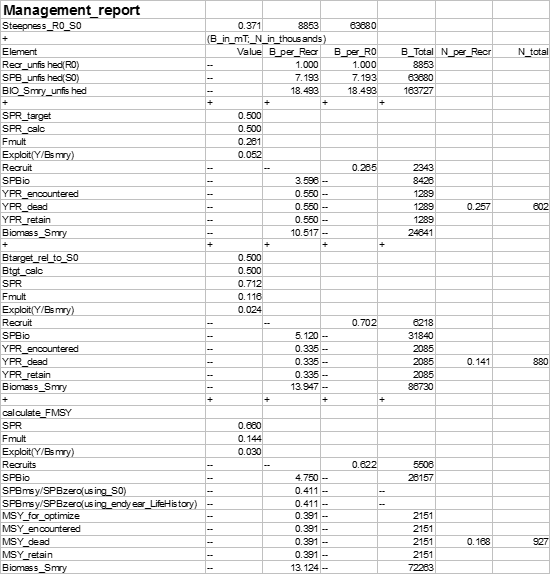
\includegraphics{ManagementReport}
%\end{center}


%\begin{landscape}
%The forecast is done once using the Target SPR and once using the adjustments specified in the 40:10 section of forecast.ss input. Each section contains a time series of seasonal biomass and catch, followed by a time series of population numbers-at-age for each platoon.
	
%	\begin{center}
%		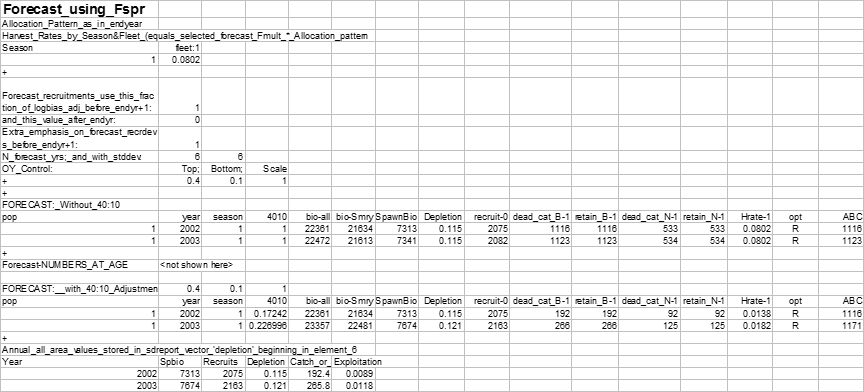
\includegraphics{Forecast}
%	\end{center}
%\end{landscape}

%where:
%\begin{itemize}
%	\item 40:10 is the magnitude of the adjustment of harvest multiplier to implement the optimum yield policy;
%	\item bio-all is the biomass of all ages;
%	\item bio-smry is the biomass for ages at or above the summary age;
%	\item Spawnbio - is the female spawning biomass/output;
%	\item Depletion is the spawning biomass/output divided by the unfished spawning biomass/output;
%	\item Recruit-0 is the recruitment of age-o fish in this year;
%	\item Dead\_cat\_B-1 is the total dead (retained plus dead discard) catch in MT for fleet 1;
%	\item Retain\_B-1 is fleet 1's retained catch in MT;
%	\item Equivalent catch in numbers is then reported;
%	\item Hrate-1 is the harvest rate, as adjusted by the 40:10 policy.  The units will depend on the F method selected (Pope's method giving mid-year harvest rate or the continuous F).
%	\item Opt=C means that the rate was calculated from an input catch level (and crashed means that this caused an excessive harvest rate.
%	\item Opt=R means that the catch was calculated from the target harvest rate.; and
%	\item ABC is equal to the Total-Catch when the 40:10 option is not used (upper portion of table).  When the 40:10 is on (lower table), the ABC is the catch level corresponding to no 40:10 adjustment after accounting for catch in previous year's from the 40:10.
%\end{itemize}

%The time series output described above is detailed by season, area, platoon and fishery.  It is usually more convenient to have annual values summed across areas, platoons and fisheries.  This is done for the 40:10 output and a subset of these values are replicated in the depletion vector in the sd\_report so that variance estimates can be obtained.  The elements of the depletion vector in the sd\_report are:
%\begin{itemize}
%	\item depletion level in end year
%	\item depletion level in end year+1
%	\item MSY (if calculated, else spbio in endyr-1)
%	\item B\textsubscript{MSY} (if calculated, else spbio in endyr)
%	\item SPR\textsubscript{MSY} (if calculated, else spbio in endyr+1) then the time series of:
%	\begin{itemize}
%		\item Spawning biomass
%		\item Recruitment
%		\item Depletion level
%		\item Total catch (if forecast calculated catch from rates) or sum of fishery-specific harvest rates (if forecast is based on fixed input catch level in this year)
%		\item Total exploitation rate (total dead catch divided by the summary biomass at the beginning of the year).
%	\end{itemize}
%\end{itemize}

%\begin{center}
%	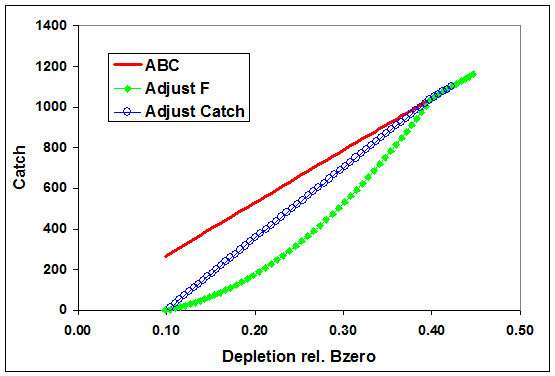
\includegraphics{HCR}\\
%	Two examples of harvest forecast adjustment: one adjusts catch and the other adjusts F.
%\end{center}

\subsection{Main Output File, Report.sso}
This is the primary output file.  Its major sections are listed below.  

The sections of the output file are:
\begin{itemize}
	\item SS version number with date compiled.  Time and date of model run.  This info appears at the top of all output files.
	\item Comments
		\begin{itemize}
			\item 	Input file lines starting with \#C are echoed here.
		\end{itemize}
	\item Keywords
		\begin{itemize}
			\item List of keywords used in searching for output sections.
		\end{itemize}
	\item Fleet Names
		\begin{itemize}
			\item List of fishing fleet and survey names assigned in the data file.
		\end{itemize}
	\item Likelihood
		\begin{itemize}
			\item Final values of the negative log(likelihood) are presented.
		\end{itemize}
	\item Input Variance Adjustments
		\begin{itemize}
			\item The matrix of input variance adjustments is output here because these values affect the log likelihood calculations.
		\end{itemize}
	\item Parameters
		\begin{itemize}
			\item The parameters are listed here.  For the estimated parameters, the display shows: Num (count of parameters), Label (as internally generated by SS), Value, Active\_Cnt, Phase, Min, Max, Init, Prior, Prior\_type, Prior\_SD, Prior\_Like, Parm\_StD (standard deviation of parameter as calculated from inverse Hessian), Status (e.g. near bound), and Pr\_atMin (value of prior penalty if parameter was near bound).  The Active\_Cnt entry is a count of the parameters in the same order they appear in the ss.cor file.
		\end{itemize}
	\item Derived Quantities
		\begin{itemize}
			\item This section starts by showing the options selected from the starter.ss and forecast.ss input files:
				\begin{itemize}
					\item SPR ratio basis
					\item F report basis
					\item B ratio denominator
				\end{itemize}
		\end{itemize}
\end{itemize}

Then the time series of output, with standard deviation of estimates, are produced with internally generated labels.  Note that these time series extend through the forecast era.  The order of the output is: spawning biomass, recruitment, SPRratio, Fratio, Bratio, management quantities, forecast catch (as a target level), forecast catch as a limit level (OFL), Selex\_std, Grow\_std, NatAge\_std.  For the three "ratio" quantities, there is an additional column of output showing a Z-score calculation of the probability that the ratio differs from 1.0. The "management quantities" section is designed to meet the terms of reference for west coast groundfish assessments; other formats could be made available upon request. The standard deviation quantities at the end are set up according to specifications at the end of the control input file. In some cases, a user may specify that no derived quantity output of a certain type be produced. In those cases, SS substitutes a repeat output of the virgin spawning biomass so that vectors of null length are not created.

ADMB note, while vectors of null length are very useful for controlling optional model inputs, they cannot be used with current version of ADMB for sdreport quantities.

\begin{itemize}
	\item Mortality-growth parameter by year after adjustments
	\begin{itemize}
		\item This block shows the time series of mortality-growth parameters by year after adjustment by environmental links, blocks and deviations.
	\end{itemize}
	\item Selectivity parameters (size) by year after adjustments
	\begin{itemize}
		\item This block shows the size selectivity parameters, after adjustment, for each year in which a change occurs.
	\end{itemize}
	\item Selectivity parameters (age) by year after adjustments
	\begin{itemize}
		\item This block shows the age selectivity parameters, after adjustment, for each year in which a change occurs.
	\end{itemize}
	\item Recruitment Distribution
	\begin{itemize}
		\item This block shows the distribution of recruitment across growth patterns, genders, birth seasons, and areas in the end year of the model.
	\end{itemize}
	\item Platoon Indexing
	\begin{itemize}
		\item This block shows the internal index values for various quantities.  It can be a useful reference for complex model setups. The vocabulary is: Bio\_Pattern refers to a collection of cohorts with the same defined growth and natural mortality parameters; sex is the next main index. If recruitment occurs in multiple seasons, then birth season is the index for that factor. The index labeled "Platoon" is used as a continuous index across all the other factor-specific indices. If sub-platoons are used, they are nested within the Bio\_Pattern x Sex x Birth Season platoon. However, some of the output tables use the column label "platoon" as a continuous index across platoons and sub-platoons. Note that there is no index here for area. Each of the cohorts is distributed across areas and they retain their biological characteristics as they move among areas.
	\end{itemize}
	\item Size Frequency Translation
	\begin{itemize}
		\item If the generalized size frequency approach is used, this block shows the translation probabilities between population length bins and the units of the defined size frequency method.  If the method uses body weight as the accumulator, then output is in corresponding units.
	\end{itemize}
	\item Movement
	\begin{itemize}
		\item This block shows movement rate between areas in a multi-area model.
	\end{itemize}
	\item Exploitation
	\begin{itemize}
		\item This block shows the time series of the selected F\_std unit and the F multiplier for each fleet in terms of harvest rate (if Pope's approximation is used) or fully selected F.
	\end{itemize}
	\item Index 2
	\begin{itemize}
		\item This section reports the observed and expected values for each index. All are reported in one list with index number included as a selection field. At the bottom of this section, the root mean squared error of the fit to each index is compared to the mean input error level to assist the user in gauging the goodness-of-fit and potentially adjusting the input level of imprecision.
	\end{itemize}
	\item Index 3
	\begin{itemize}
		\item This section shows the parameter number assigned to each parameter used in this section.
	\end{itemize}
	\item Discard
	\begin{itemize}
		\item This is the list of observed and expected values for the amount (or fraction) discard.
	\end{itemize}
	\item Mean Body Wt
	\begin{itemize}
		\item This is the list of observed and expected values for the mean body weight.
	\end{itemize}
	\item Fit Len Comps
	\begin{itemize}
		\item This is the list of the goodness of fit to the length compositions. The input and output levels of effective sample size are shown as a guide to adjusting the input levels to better match the model's ability to replicate these observations.
	\end{itemize}
	\item Fit Age Comps
	\begin{itemize}
		\item This has the same format as the length composition section.
	\end{itemize}
	\item Fit Size Comps
	\begin{itemize}
		\item This has the same format as the length composition section and is used for the generalized size composition summary.
	\end{itemize}
	\item Len Selex
	\begin{itemize}
		\item Here is the length selectivity and other length specific quantities for each fishery and survey.
	\end{itemize}
	\item Age Selex
	\begin{itemize}
		\item Here is reported the time series of age selectivity and other age-related quantities for each fishery and survey. Some are directly computed in terms of age, and others are derived from the combination of a length-based factor and the distribution of size-at-age.
	\end{itemize}
	\item Environmental Data
	\begin{itemize}
		\item The input values of environmental data are echoed here. In the future, the summary biomass in the previous year will be mirrored into environmental column –2 and that the age zero recruitment deviation into environmental column –1. Once so mirrored, they may enable density-dependent effects on model parameters.
	\end{itemize}
	\item Numbers at Age
	\begin{itemize}
		\item The output (in thousands of fish) is shown for each cohort tracked in the model.
	\end{itemize}
	\item Numbers at Length
	\begin{itemize}
		\item The output is shown for each cohort tracked in the model.
	\end{itemize}
	\item Catch at Age
	\begin{itemize}
		\item The output is shown for each fleet.  It is not necessary to show by area because each fleet operates in only one area.
	\end{itemize}
	\item Biology
	\begin{itemize}
		\item The first biology section shows the length-specific quantities in the ending year of the time series only. The derived quantity spawn is the product of female body weight, maturity and fecundity per weight. The second section shows natural mortality.
	\end{itemize}
	\item Growth Parameters
	\begin{itemize}
		\item This section shows the growth parameters, and associated derived quantities, for each year in which a change is estimated.
	\end{itemize}
	\item Biology at Age
	\begin{itemize}
		\item This section shows derived size-at-age and other quantities. It is the basis for the Bio report page of the Excel output processor.
	\end{itemize}
	\item Mean Body Wt (begin)
	\begin{itemize}
		\item This section reports the time series of mean body weight for each platoon. Values shown are for the beginning of each season of each year.
	\end{itemize}
	\item Mean Size Time series
	\begin{itemize}
		\item This section shows the time series of mean length-at-age for each platoon. At the bottom is the average mean size as the weighted average across all platoons for each gender.
	\end{itemize}
	\item Age Length Key
	\begin{itemize}
		\item This is reported for the midpoint of each season in the ending year.
	\end{itemize}
	\item Age Age Key
	\begin{itemize}
		\item This is the calculated distribution of observed ages for each true age for each of the defined ageing keys.
	\end{itemize}
	\item Selectivity Database
	\begin{itemize}
		\item This section contains the selectivities organized as a database, rather than as a set of vectors.
	\end{itemize}
	\item Spawning Biomass Report 2, etc.
	\begin{itemize}
		\item The section shows annual total spawning biomass, then numbers-at-age at the beginning of each year for each Bio\_Pattern and Sex as summed over sub-platoons and areas.  Then Z-at-age is reported simply as $ln(N_{t+1,a+1} N_{t,a})$.  Then the Report\_1 section loops back through the time series with all F values set to zero so that a dynamic Bzero, N-at-age, and M-at-age can be reported.  The difference between Report\_1 and Report\_2 can be used to create an aggregate F-at-age.
	\end{itemize}
	\item Composition Database
	\begin{itemize}
		\item This section is reported to a separate file, compreport.sso, and contains the length composition, age composition, and mean size-at-age observed and expected values.  It is arranged in a database format, rather than an array of vectors.  Software to filter the output allows display of subsets of the database.
	\end{itemize}
\end{itemize}

\pagebreak
	
	%========= Section 14: R4SS
	
\section{Using R To View Model Output (r4ss)}\label{r4ss}

A collection of functions developed as a package, \texttt{r4ss}, for the statistical software R has been created to explore SS model output.  The functions include tools for summarizing and plotting results, manipulating files, visualizing model parameterizations, and various other tasks.  Currently, information on the code, including installation instructions, can be found at github.com/r4ss/r4ss.  The software package is under constant development to maintain compatibility with new versions of SS and to improve functionality.

Two of the most commonly used functions for model diagnostics are \texttt{SS\_output} and \texttt{SS\_plots}.  After running a model using SS, the report can be read into R by the \texttt{SS\_output} function which stores quantities in a list with named objects.  This list can then be passed to the \texttt{SS\_plots} function which creates a series of over 100 plots that are useful to visualize output such as model fit to the data and time series of quantities of interest.

The latest \texttt{r4ss} version on CRAN can be installed using a command like:

\begin{quote}
	\begin{verbatim}
	> install.packages("r4ss")
	\end{verbatim}
\end{quote}


However, more frequent enhancements and bug fixes are posted to the GitHub project.  The latest version of \texttt{r4ss} can be installed directly from GitHub at any time via the \texttt{devtools} package in R with the following commands:

\begin{quote}
	\begin{verbatim}
	> install.packages("devtools")
	> devtools::install_github("r4ss/r4ss")
	\end{verbatim}
\end{quote}

Note: \texttt{devtools} will give this message: \textit{"WARNING: Rtools is required to build R packages, but is not currently installed."}. However, \texttt{Rtools} is not required for installing \texttt{r4ss} via \texttt{devtools}, so ignore this warning.

Once you have installed the \texttt{r4ss} package, it can be loaded in the regular manner:

\begin{quote}
	\begin{verbatim}
	> library(r4ss)
	\end{verbatim}
\end{quote}


The results from a model run can be read in and plots created using the following commands:

\begin{quote}
	\begin{verbatim}
	> setwd("C:\directory where model was run")
	> base.model = SS_output(getwd())
	> SS_plots(base.model)
	\end{verbatim}
\end{quote}

The \texttt{SS\_output()} function reads the Report file and stores this information in a list. The function by default will print select items to the screen that can be useful for evaluating a model (e.g., likelihood, estimated parameter with warnings if they hit bounds, parameters with high gradients). This list created by \texttt{SS\_output()} can be passed to other functions in the \texttt{r4ss} package to allow visualization of results.
%\pagebreak
%Example of the data displayed used by the SS\_output function:
%\begin{center}
%		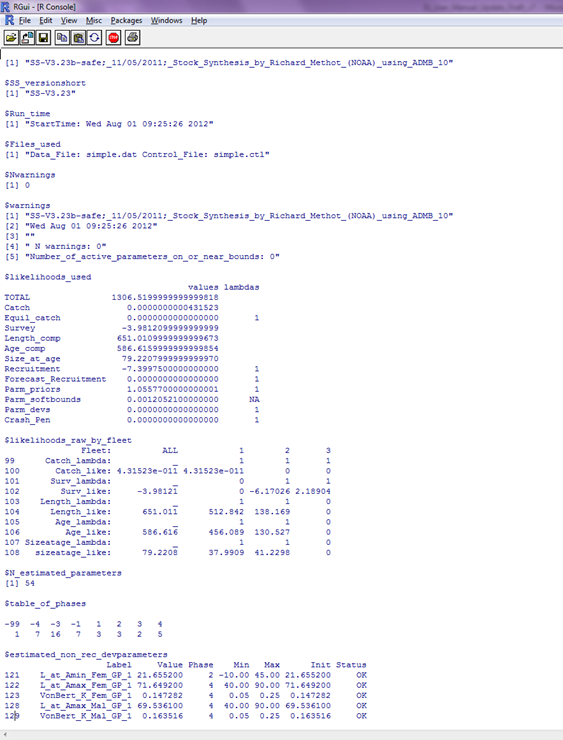
\includegraphics{r4ss_output}
%\end{center}

%\pagebreak
The \texttt{SS\_plots()} function will create plots from the list created by the \texttt{SS\_output()} function that can be used to visualize model results.  The plots by default will be written inside a "plots" folder inside the folder with the model files read by the \texttt{SS\_output()} function.  Additionally, an html file is written which allows for visualization of all plots created.   

%Example of the plots created using the SS\_plots function:
%\begin{center}
%	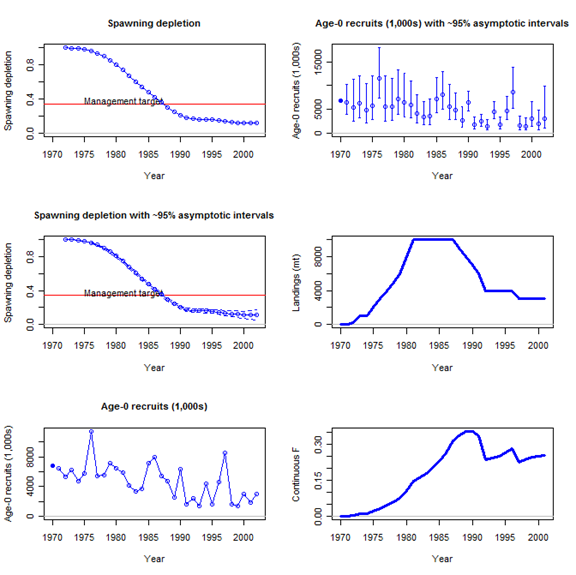
\includegraphics{r4ss_plots}
%\end{center}

%\pagebreak
The functions included in r4ss ranging from general use to functions developed for specific model applications:
\begin{center}
	\begin{longtable}{p{4.5cm} p{10.52cm}}
		\hline
		Core Functions & \Tstrut\Bstrut\\
		\hline
		SS\_output \Tstrut& A function to create a list object for the output from Stock Synthesis\\
		SS\_plots  \Tstrut& Plot many quantities related to output from Stock Synthesis\\
		\hline
		
		\multicolumn{2}{l}{Plot functions called by SS\_plots:} \Tstrut\Bstrut\\
		\hline
		SSplotBiology \Tstrut& Plot biology related quantities from Stock Synthesis model output, including mean weight, maturity, fecundity, and spawning output. \\
		SSplotCatch   \Tstrut & Plot catch related quantities \\
		SSplotCohorts \Tstrut & Plot cumulative catch by cohort \\
		SSplotComps   \Tstrut & Plot composition data and fits \\
		SSplotData    \Tstrut & Timeline of presence/absence data by type, year, and fleet \\
		SSplotDiscard \Tstrut & Plot fit to discard fraction \\
		SSplotIndices \Tstrut & Plot indices of abundance and associated quantities \\
		SSplotMnwt    \Tstrut & Plot mean weight data and fits \\
		SSplotMovementMap \Tstrut & Show movement rates on a map \\
		SSplotMovementRates \Tstrut & Show movement rates on a map \\
		SSplotNumbers \Tstrut& Plot numbers-at-age related data and fits \\
		SSplotRecdevs \Tstrut& Plot recruitment deviations \\
		SSplotRecdist \Tstrut& Plot of recruitment distribution among areas and seasons \\
		SSplotSelex   \Tstrut& Plot selectivity \\
		SSplotSexRatio \Tstrut& Plot sex ratios \\
		SSplotSummaryF \Tstrut& Plot time series summary of F (or harvest rate) \\
		SSplotSpawnrecruit \Tstrut& Plot spawner-recruit curve \\
		SSplotSPR     \Tstrut& Plot SPR quantities \\
		SSplotTags    \Tstrut& Plot tagging data and fits \\
		SSplotTimeseries \Tstrut& Plot time series data \\
		SSplotYield   \Tstrut& Plot yield and surplus production \\
		SS\_html \Tstrut& Create HTML files to view figures in browser \\
		SS\_fitbiasramp \Tstrut& Estimate bias adjustment for recruitment deviates \Bstrut\\
		\hline
	
		\multicolumn{2}{l}{Model Comparisons and other diagnostics:} \Tstrut\Bstrut\\
		\hline
		SSplotPars    \Tstrut & Plot distributions of priors, posteriors, and estimates \\
		SSplotProfile \Tstrut & Plot likelihood profile results \\
		PinerPlot     \Tstrut & Plot fleet-specific contributions to likelihood profile \\
		SSplotRetroRecruits \Tstrut & Make retrospective pattern of recruitment estimates (a.k.a. squid plot) as seen in Pacific hake assessments\Bstrut \\
		\hline
		
		\multicolumn{2}{l}{Functions related to MCMC diagnostics:}\Tstrut\Bstrut\\
		\hline
		mcmc\_nuisance \Tstrut & Summarize nuisance MCMC output \\
		mcmc\_out      \Tstrut & Summarize, analyze, and plot key MCMC output \\
		SSgetMCMC      \Tstrut & Read MCMC output \\
		SSplotMCMC\_ExtraSelex \Tstrut & Plot uncertainty around chosen selectivity ogive from MCMC \Bstrut\\
		\hline
		
		\multicolumn{2}{l}{Interactive tools for exploring functional forms:} \Tstrut\Bstrut\\
		\hline
		movepars    \Tstrut  & Explore movement parameterization \\
		selfit      \Tstrut  & A function to visualize parameterization of double normal and double logistic selectivity in SS \\
		selfit\_spline \Tstrut & Visualize parameterization of cubic spline selectivity in SS \\
		sel\_line   \Tstrut & A function for drawing selectivity curves\Bstrut \\
		\hline


		\multicolumn{2}{l}{File manipulation for inputs:}\Tstrut\Bstrut\\
		\hline
		SS\_readdat  \Tstrut & Read data file \\
		SS\_readforecast \Tstrut & Read forecast file \\
		SS\_readstarter  \Tstrut & Read starter file \\
		SS\_writedat  \Tstrut & Write data file \\
		SS\_writeforecast \Tstrut & Write forecast file \\
		SS\_writestarter  \Tstrut & Write starter file \\\Tstrut 
		SS\_makedatlist   \Tstrut & Make a list for SS data \\
		SS\_parlines    \Tstrut & Get parameter lines from SS control file \\
		SS\_changepars  \Tstrut  & Change parameters in the control file \\
		SSmakeMmatrix    \Tstrut & Create inputs for entering a matrix of natural mortality by age and year \\
		SS\_profile      \Tstrut & Run a likelihood profile in SS (incomplete) \\
		NegLogInt\_Fn     \Tstrut& Calculated variances of time-varying parameters using SS implementation of the Laplace Approximation \Bstrut\\
		\hline

		\multicolumn{2}{l}{File manipulations for outputs:}\Tstrut\Bstrut\\
		\hline
		SS\_recdevs  \Tstrut & Insert a vector of recruitment deviations into the control file \\
		SS\_splitdat \Tstrut & Split apart bootstrap data to make input file \Bstrut\\
		\hline

		\multicolumn{2}{l}{Minor plotting functions:}\Tstrut\Bstrut\\
		\hline
		bubble3         \Tstrut & Create a bubble plot \\
		make\_multifig  \Tstrut & Create multi-figure plots \\
		Make\_multifig\_sexratio \Tstrut & Create multi-figure plots of sex ratios \\
		plotCI          \Tstrut & Plot points with confidence intervals \\
		rich\_colors\_short \Tstrut & Make a vector of colors \\
		stackpoly       \Tstrut & Plot stacked polygons \\
		mountains       \Tstrut & Make shaded polygons with a mountain-like appearance \Bstrut\\
		
		\hline
		\multicolumn{2}{l}{Really specialized functions:} \Tstrut\Bstrut\\
		\hline
		DoProjectPlots \Tstrut & Make plots from Rebuilder program \\
		IOTCmove       \Tstrut & Make a map of movement for a 5-area Indian Ocean model \\
		SSFishGraph    \Tstrut & A function for converting SS output to the format used by FishGraph \\
		TSCplot        \Tstrut & Create a plot for the TSC report \Bstrut\\
		\hline
	\end{longtable}
\end{center}
	
	%========= Section 15: Special Set-ups
	\section{Special Set-ups}

\subsection{Continuous seasonal recruitment}
It is awkward in SS to set up a seasonal model such that recruitment can occur with similar and independent probability in any season of any year.  Consequently, some users have attempted to setup SS so that each quarter appears as a year.  They have set up all the data and parameters to treat quarters as if they were years (i.e. each still has a duration of 1.0 time step).  This can work, but requires that all rate parameters be re-scaled to be correct for the quarters being treated as years.

Another option is available.  If there is one season per year and the season duration is set to 3 (rather than the normal 12), then the season duration is calculated to be 3/12 or 0.25.  This means that the rate parameters can stay in their normal per year scaling and this shorter season duration makes the necessary adjustments internally.  Some other adjustments to make when doing quarters as years include:

\begin{itemize}
	\item re-index all "year seas" inputs to be in terms of quarter-year because all are now season 1; increase endyr value in sync with this
	\item increase max age because age is now in quarters
	\item in the age error definitions, increase the number of entries in accord with new max age
	\item in the age error definitions, recode so that each quarter-age gets assigned to the correct agebin;  This is because the age data are still in terms of agebins; i.e. the first 4 entries for quarter-ages 1 through 4 will all be assigned to agebin 1.5; the next four to agebin 2.5;  you cannot accomplish the same result by editing the age bin values because the stddev of ageing error is in terms of agebin
	\item in the control file, multiple the natM age breakpoints  and growth AFIX values by 1/seasdur
	\item decrease the R0 parameter starting value because it is now the average number of recruitments per quarter year
	\item edit the rec\_dev start and endyrs to be in terms of quarter year
	\item edit any age selectivity parameters that refer to age to now refer to quarter age
	\item if there needs to be some degree of seasonality to recruitment or some parameter, then you could create a cyclic pattern in the environmental input and make recruitment or some other parameter a function of this cyclic pattern
\end{itemize}
	
A good test showing comparability of the 3 approaches to setting up a quarterly model should be done.


	%========= Section 16: Essays
	\hypertarget{PopDyModeling}{}
\section[Guidance on Population Dynamics Modeling]{\protect\hyperlink{PopDyModeling}{Guidance on Population Dynamics Modeling}}

Numerous assessment related topics have arisen among users. A collection of general information on population dynamics modeling is provided here. This information is relative to both users of SS3 and users of other stock assessment modeling platforms.

%=========Data Weighting
\subsection{Data Weighting}
\label{sec:DataWeight}
\hypertarget{DataWeight}{}


In 2015 there was a CAPAM workshop dedicated to data-weighting. Description of the workshop can be found on the \href{http://capamresearch.org/data-weighting/workshop}{CAPAM} website. The presentations from the workshop are available through that website and many of them were included in a special issue of \href{https://sciencedirect.com/journal/fisheries-research/vol/192}{Fisheries Research}.


Currently, there are three main methods for weighting length and data applied for U.S. West Coast assessments using Stock Synthesis.

\begin{enumerate}
	\item \textbf{McAllister - Ianelli}: Effective sample size is calculated from fit of observed to expected length or age compositions. Tuning algorithm is intended to make the arithmetic mean of the input sample size equal to the harmonic mean of the effective sample size \citep{mcallister_bayesian_1997}.
	
	\item \textbf{Francis}: Based on variability in the observed mean length or age by year, where the sample sizes are adjusted such that the fit of the expected mean length or age should fit within the uncertainty intervals at a rate which is consistent with variability expected based on the adjusted sample sizes (Method "TA1.8") \citep{francis_data_2011}
	
	\item \textbf{Dirichlet-Multinomial}: A new likelihood (as opposed to the standard multinomial) which includes an estimable parameter (theta) which scales the input sample size. In this case, the term "Effective sample size" has a different interpretation than in the McAllister-Ianelli approach \citep{thorson_model-based_2017}.
\end{enumerate}

\myparagraph{Applying the methods}

%\subsubsection{McAllister-Ianelli}
\myparagraph{McAllister-Ianelli}
The "Length\_Comp\_Fit\_Summary" and "Age\_Comp\_Fit\_Summary" sections in the Report file include information on the harmonic mean of the effective sample size and arithmetic mean of the input sample size used in this tuning method. In the r4ss package, these tables are returned by the \texttt{SS\_output} function as \texttt{ \$Length\_comp\_Eff\_N\_tuning\_check} and \texttt{ \$Age\_comp\_Eff\_N\_tuning\_check}.

A convenient way to process these values into the format required by the control file is to use the function:

\texttt{ SS\_tune\_comps(replist, option = "MI") }

where the input "replist" is the object created by \texttt{SS\_output}. This function will return a table and also write a matching file called "suggested\_tuning.ss" to the directory where the model was run.

For models using SS version 3.30, the table created by \texttt{SS\_tune\_comps} can be pasted into the bottom of the control file in the section labeled "Input variance adjustments", followed by the terminator line which indicates the end of the section. 

%Here's an example of the first few rows of the table followed by the terminator line (not added by the function):

%\begin{center}
%	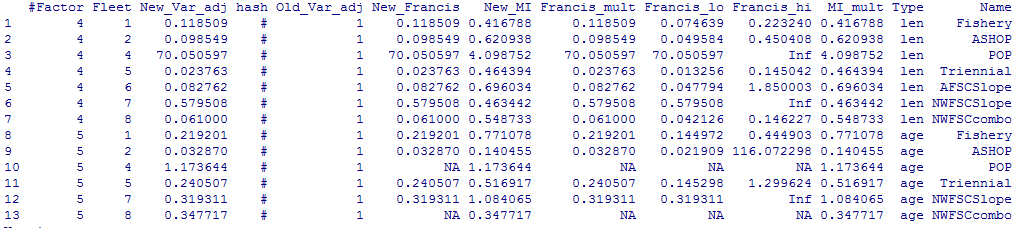
\includegraphics[scale = 0.6]{appendixB_sstune}\\
%\end{center}

Also see the help page for the r4ss function \texttt{SS\_varadjust} which can be used to automatically write a new control file if you want to streamline the process of applying multiple iterations of this tuning method.

If the tuning has been implemented, the green lines in the figure below would approximately intersect at a point which is on the black 1-to-1 diagonal line in this figure created by the r4ss function \texttt{SS\_plots}.

\begin{figure}[h]
	\begin{center}
		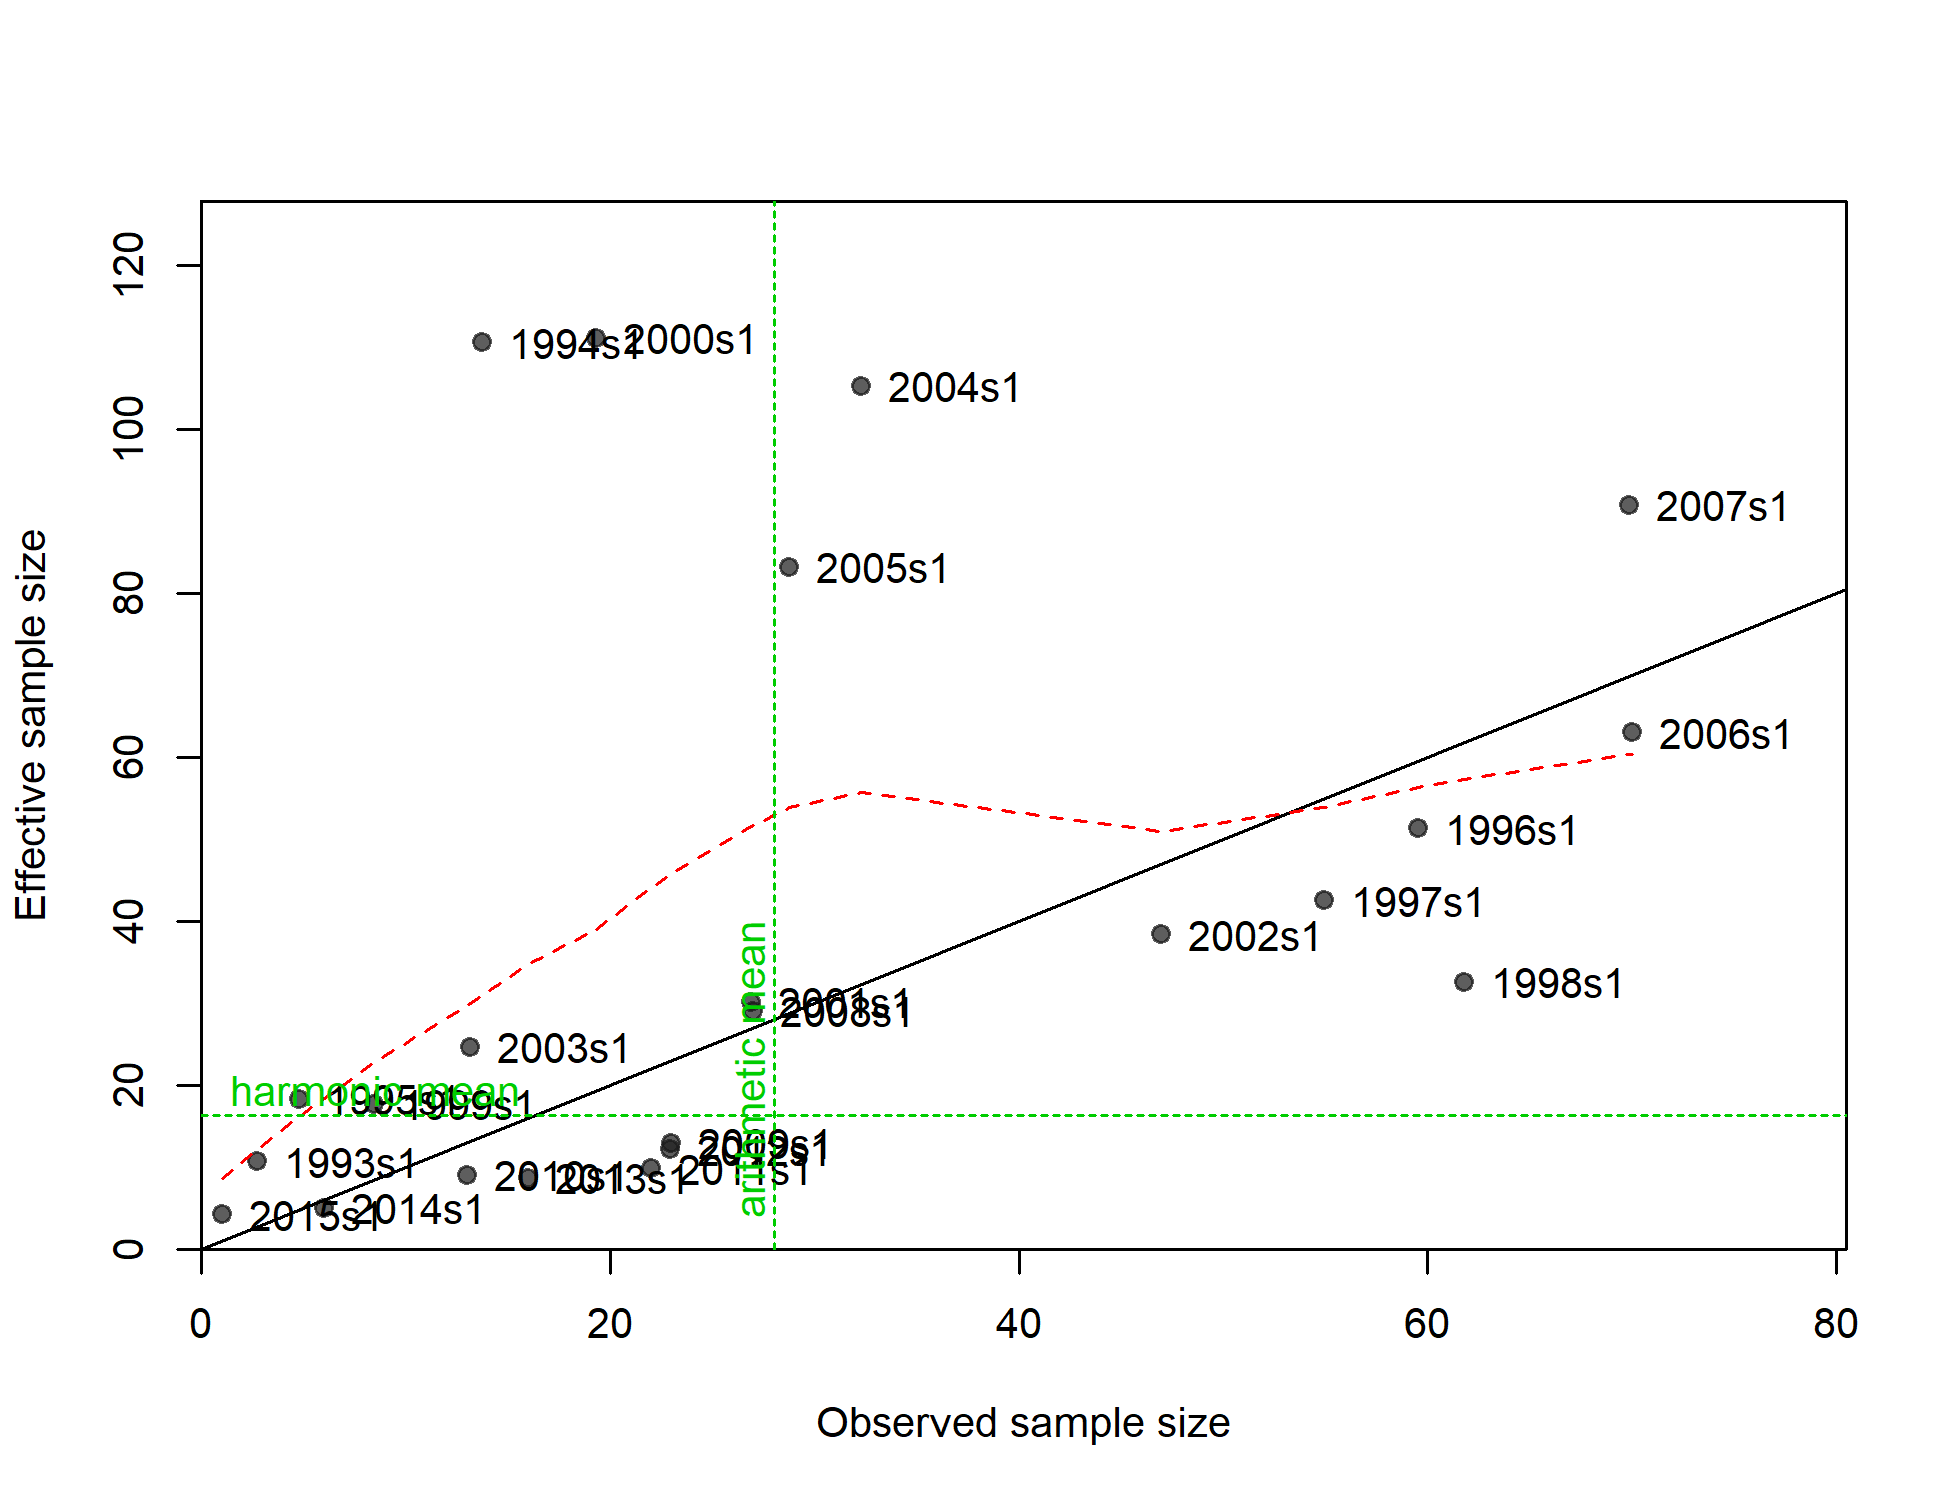
\includegraphics[scale = 0.65]{appendixB_McAllister_Ianelli}\\
	\end{center}

	\caption{ The relationship between the observed sample size (the input sample number) versus the effective sample size where the effective sample size is the product of the input sample size and the data weighting applied to the data set. }
	\label{(fig:mcallister)}
\end{figure}

There are a couple of challenges posed by the McAllister-Ianelli data-weighting approach:
\begin{enumerate}
	\item Subjective choice of how many iterations to take to achieve adequate convergence. Often just one iteration is applied.
	
	\item Takes time to implement so tuning is rarely repeated during retrospective or sensitivity analyses.
\end{enumerate}

%\subsubsection{Francis}
\myparagraph{Francis}

Implementation: recommended adjustments are calculated by the r4ss functions \texttt{SSMethod.TA1.8} and \texttt{SSMethod.Cond.TA1.8}. These functions are rarely used alone but are called by the \texttt{SS\_plots} function when making plots like the one below. For SS v.3.30 models, the simplest way to get the adjustments in the format required by the control file is to use the \texttt{SS\_tune\_comps} function (described above under the McAllister-Ianelli method), but with a different option specified: 

\texttt{SS\_tune\_comps(replist, option = "Francis")}

The figure below shows the estimated 95\% intervals around the observed mean length by year based on the input sample size (thick lines) and the increase in that uncertainty which would occur if the sample sizes were adjusted according to the proposed multiplier.

\begin{figure}[h]
	\begin{center}
		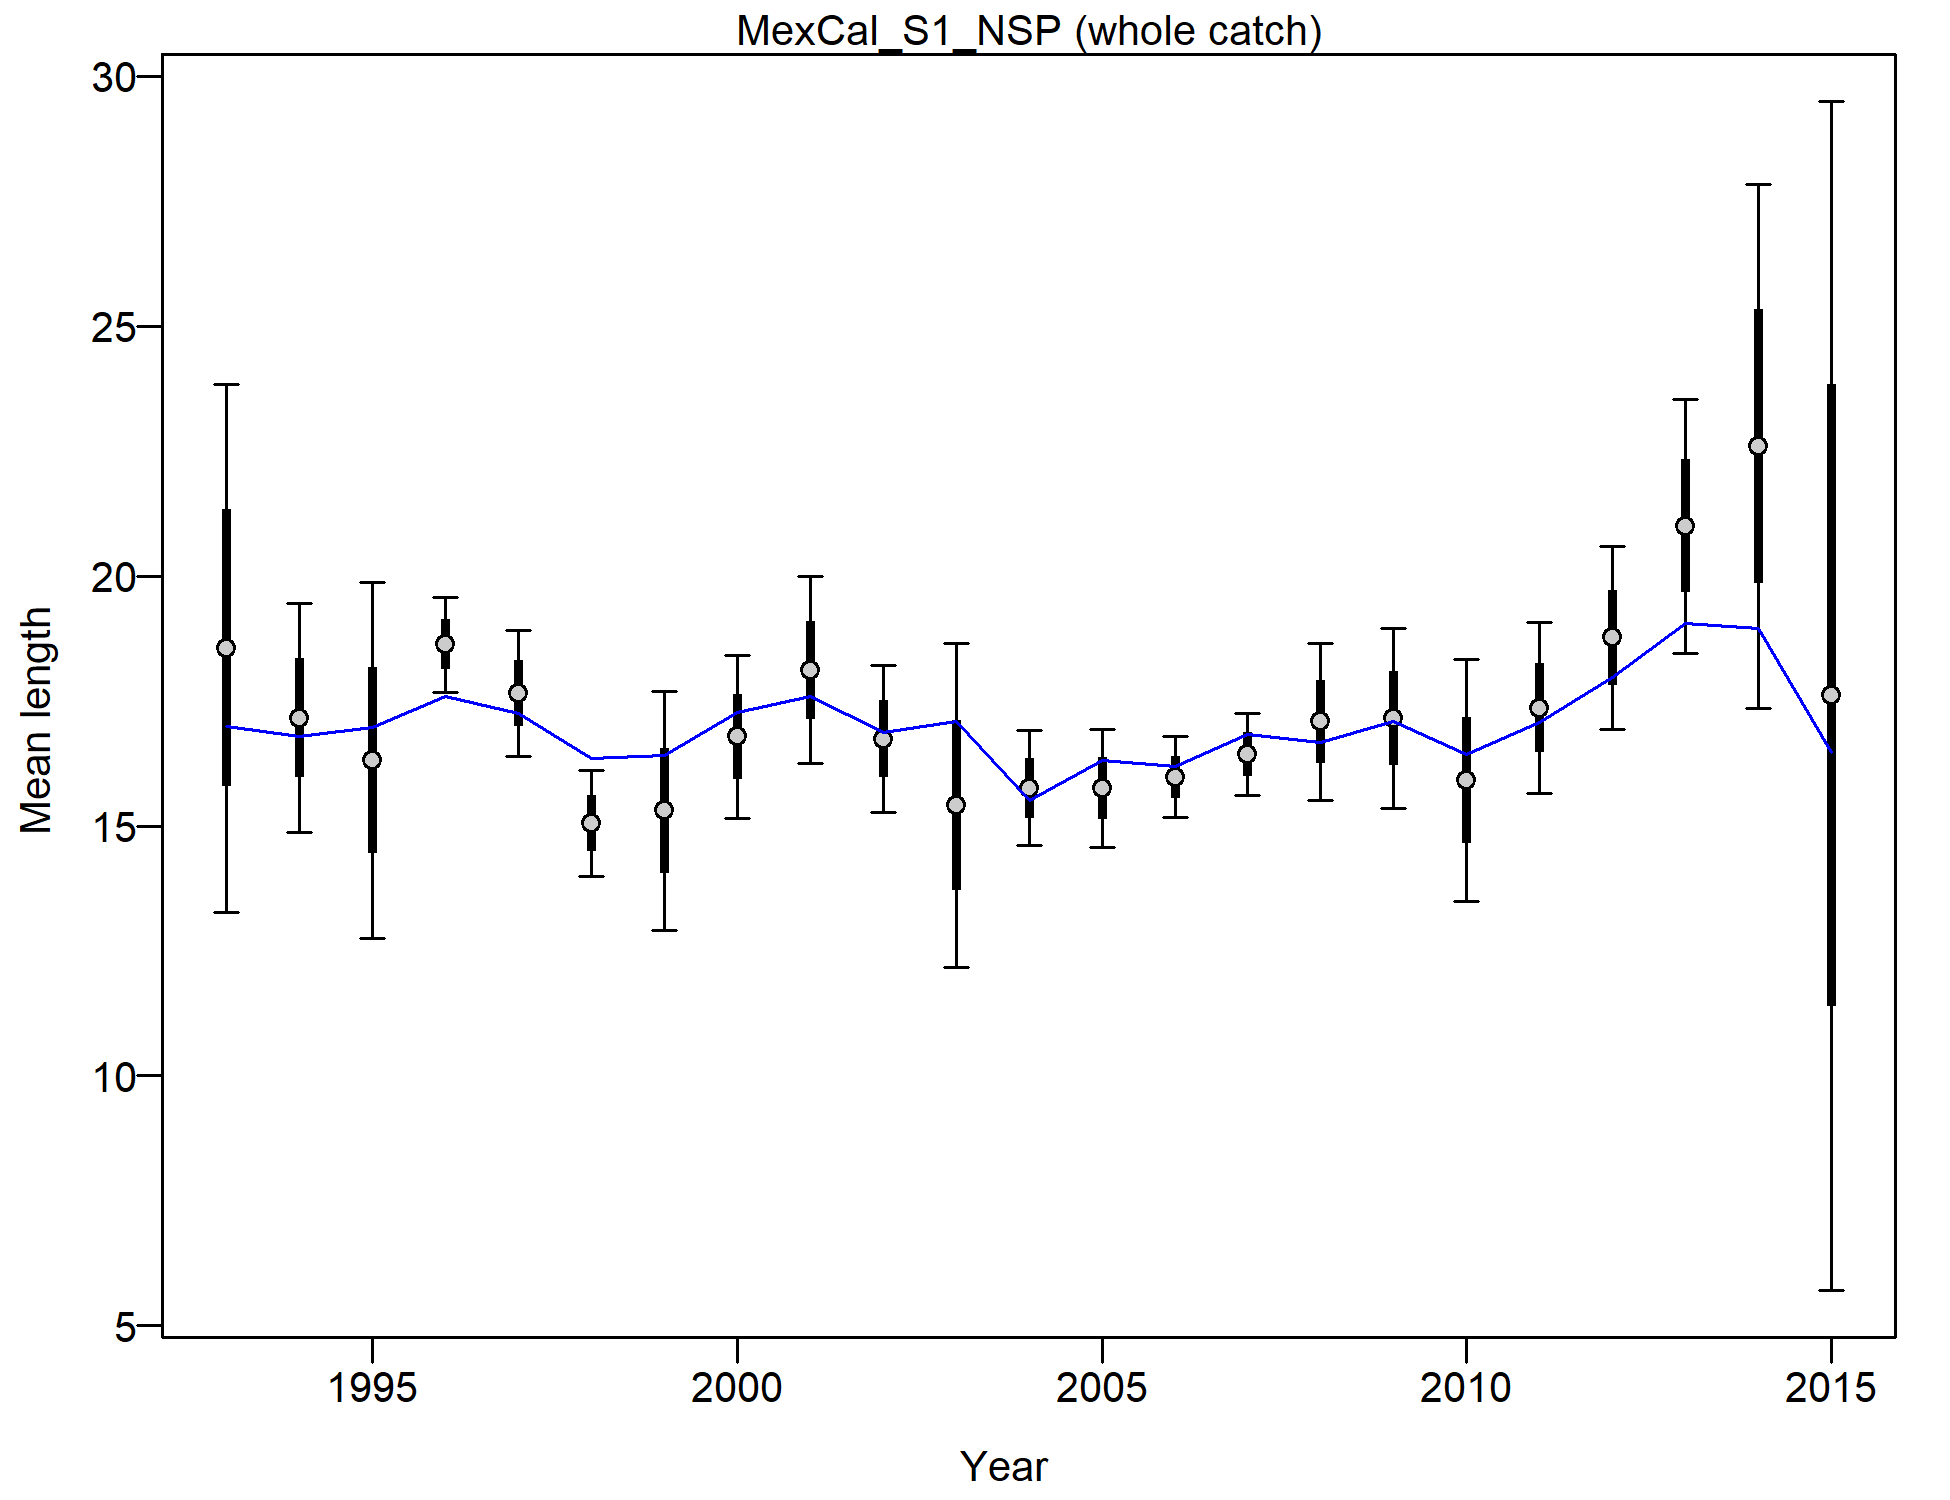
\includegraphics[scale = 0.15]{appendixB_Francis}\\
	\end{center}
	\caption{The mean length of the length samples for each year from Fleet 1 (called the MexCal S1 NSP fleet) with 95\% confidence intervals based on current samples sizes using the Francis data weighting method (referred to as TA1.8). Thinner intervals with capped ends show result of further adjusting sample sizes based on suggested multiplier, 0.2739, with 95\% interval (0.1661-0.6305) for length data from Fleet 1. The blue line shows the expected variation of the mean length across years.}
	\label{fig:francis}
	%\figurename{name}
\end{figure}



There are a several of challenges posed by the Francis data-weighting approach:
\begin{enumerate}
	\item Subjective choice of how many iterations to take to achieve adequate convergence. Often just one iteration is applied.
	
	\item Takes time to implement so tuning is rarely repeated during retrospective or sensitivity analyses.
	
	\item Recommended adjustment can be sensitive to outliers (remove a few years of anomalous composition data can lead to large change in recommended adjustment).
\end{enumerate}

%\subsubsection{Dirichlet-Multinomial}
\myparagraph{Dirichlet-Multinomial}

Change the choice of likelihood and set parameter choices in the data file:

\begin{itemize}
	\item In the specification of the length and/or age data, change "CompError" column in age and length comp specifications from 0 to 1 and "ParmSelect" from 0 to a sequence of numbers from 1 to N where N is the total number of combinations of fleet and age/length.
	
	\item Resulting input should look similar to:
	\begin{center}
		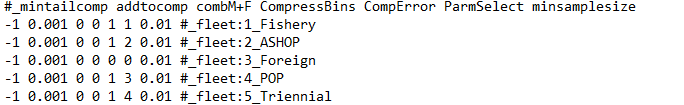
\includegraphics[scale = 0.75]{appendixB_DM_setup}\\
	\end{center}
	
	\item The ParmSelect column can also have repeated values so that multiple fleets share the same log(theta) parameter.
	
	\item If you have both length and age data, the ParmSelect should have separate numbers for each, e.g. 1 and 2 for the length comps and 3 and 4 for the age comps for the same two fleets.
	
\end{itemize}

Add parameter lines to the control file:

\begin{itemize}
	\item Add as many parameter lines as the maximum numbers in the ParmSelect column. The new parameter lines go after the main selectivity parameters but before any time-varying selectivity parameters
	
	\item Jim Thorson initially recommended bounds of -5 to 20, with a starting value of 0
    (which corresponds to a weight of about 50\% of the input sample size). However, parameter estimates above 5 are associated with 99-100\% weight with little information in the likelihood about the parameter value. Therefore, an upper bound of 5 may help identify cases that otherwise would have convergence issues.

  \item In consultation with Jim Thorson, Ian Taylor proposed a normal $N(0, 1.813)$ prior for the \texttt{ln(DM\_parm)} parameters which to counteract the effect of the logistic transformation between this parameter and the data weighting. The 1.813 value was calculated as the standard deviation of the distribution of $log(\theta)$ values derived from starting with a uniform distribution on the weights, $weight = \theta/(1+\theta) ~ U(0,1)$, and solving for $log(\theta)$. This prior was applied to the 2020 Pacific Hake stock assessment \citep{grandin_hake_2020} and led to better MCMC convergence with relatively little impact on the maximum likelihood estimates.
	
	\item Example parameter lines are below (note that the labels have changed in SS version 3.30.15 from \texttt{ln(EffN\_mult)} to \texttt{ln(DM\_parm)}.: 
		\begin{center}
			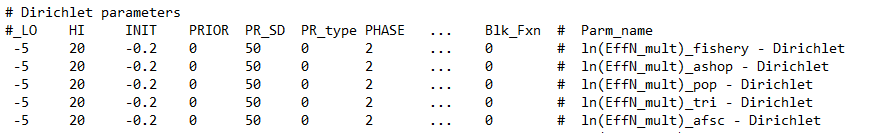
\includegraphics[scale = 0.70]{appendixB_DM_parameters}\\
		\end{center}
	
	\item Reset any existing variance adjustments factors that might have been used for the McAllister-Ianelli or Francis tuning methods. In 3.24 this means setting the values to 1, in SS version 3.30, you can simply delete or comment-out the rows with the adjustments.
\end{itemize}

The \texttt{SS\_output} function in r4ss returns table like the following:

\begin{center}
	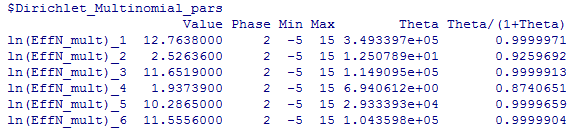
\includegraphics[scale = 1]{appendixB_DM_output}\\
\end{center}

The ratio shown in the final column is the estimated multiplier which can be compared to the sample size adjustment estimated in the other tuning methods above (the New\_Var\_adj column in the table produced by the \texttt{SS\_tune\_comps} function in r4ss).

If the reported $\theta/(1+\theta)$ ratio is close to 1.0, that indicates that the model is trying to tune the sample size as high as possible. In this case, the $ln(\theta)$ parameters should be fixed at a high value, like the upper bound of 20, which will result in 100\% weight being applied to the input sample sizes. An alternative would be to manually change the input sample sizes to a higher value so that the estimated weighting will be less than 100%.

%There is also information about this result produced in the plots created by the \texttt{SS\_plots} function:

%\begin{center}
%	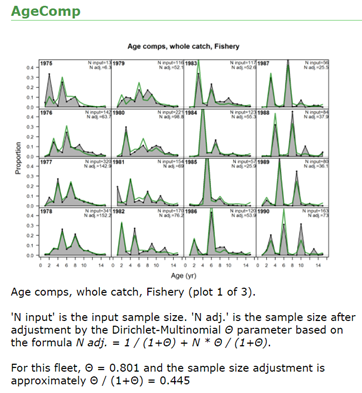
\includegraphics[scale = 1]{appendixB_DM}\\
%\end{center}

There are a several of challenges posed by the Dirichlet-Multinomial data-weighting approach:
\begin{enumerate}
	\item Not yet widely used so limited guidance is available.
	
	\item Does not allow weights above 100\% (by design) so it is not yet clear how best to deal with the situation when the estimated weight is close to 100\%.
	
	\item Parameterization has potential to cause convergence issues or inefficient MCMC sampling when weights are close to 100\% if no prior is applied as discussed above.
\end{enumerate}

%=========Recruitment Variability and Bias Adjustment
\subsection{Recruitment Variability and Bias Correction }
\hypertarget{BiasCorrect}{}

Recruitments in SS are defined as lognormal deviates around a log-bias adjusted spawner-recruitment curve.  The magnitude of the log-bias adjustment is calculated from the level of $\sigma_R$ , which is the standard deviation of the recruitment deviations (in log-space).  There are 5 segments of the time series in which to consider the effect of the log-bias adjustment: virgin; initial equilibrium; early data-poor period; data-rich period; very-recent/forecast. The choice of break points between these segments need not correspond directly with the settings for the bias adjustment, although some alignment might be desired. \citet{methot_adjusting_2011} provide more detailed discussion of the bias adjustment than what is provided below but do not address the separation of time periods into separate segments. The approach is illustrated with figures associated the assessment for darkblotched rockfish \citep{gertseva_status_2013}.

\begin{figure}
	
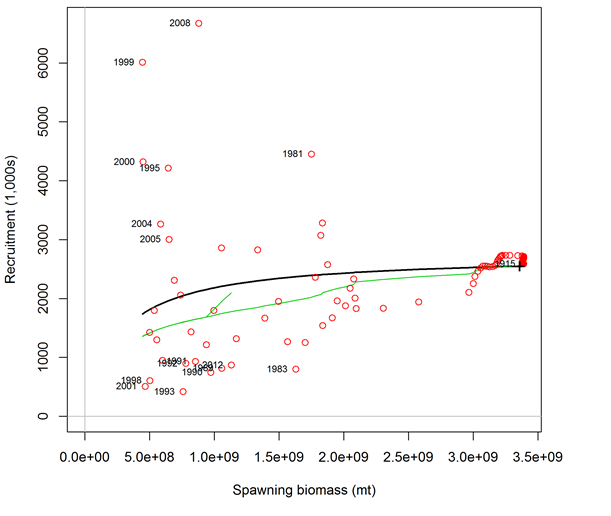
\includegraphics{appendixA_recruits}\\
\caption{ Spawner-recruitment relationship for darkblotched rockfish \citep{gertseva_status_2013}. Red points represent estimated recruitments, the solid black line is the stock-recruit relationship and the green line represents the adjustment to this relationship after adjustment to account for the lognormal distribution associated with each year. The "+" symbol labeled 1915 near the right side represents both the virgin and initial equilibrium of the model. The numerous red points close to the initial conditions correspond to the early years of the model with low harvest rates.}
\label{fig:recruits}	
\end{figure}

\begin{figure}[h]
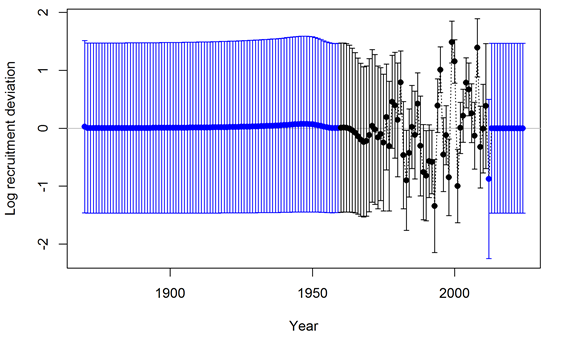
\includegraphics{appendixA_logdevs}\\
\caption{ Timeseries of log recruitment deviations for darkblotched rockfish with 95\% uncertainty intervals. The start year of the model is 1915, but recruitment deviations are estimates starting in 1870. The 45 deviation estimates for 1870–1914 inform the age structure used in the start year. The black color for the years 1960–2011 indicates the "main" recruitment deviation vector, while the blue color for the years 1870–1959 and 2012–2024 indicates the "early" and "late/forecast" recruitment deviation vectors, respectively.}
\label{fig:recdevs}
\end{figure}

\myparagraph{Virgin Biomass}
The R0 level of recruitment is a parameter of the spawner-recruitment curve.  This recruitment and the corresponding spawning biomass are expected to represent the long-term arithmetic mean.

\myparagraph{Initial Equilibrium}
The level of recruitment is typically maintained at the R0 level even though the initial equilibrium catch will reduce the spawning biomass below the virgin level. If steepness is moderately low or the initial F is high, then the lack of response in recruitment level may appear paradoxical. The logic is that building in the spawner-recruitment response to initial F would significantly complicate the calculations and would imply that the initial equilibrium catch level had been going on for multiple generations. If the lack of response is considered to be problematic in a particular application, then start the model at an earlier year and with a lower initial equilibrium catch so that the dynamics of the spawner-recruitment response get captured in the early period, rather than getting lost in the initial equilibrium.

\myparagraph{Early Data-Poor Period}
This is the early part of the time series where the only data typically are landed catch. There are no data to inform the model about the specific year-to-year fluctuations in recruitment, although the ending years of this period will begin to be influenced by the data.  The "early time period" is not a formal concept. It is up to the user to decide whether to start estimating recruitment deviations beginning with the first year of the model, or to delay such estimation until the data become more informative. Modeling recruitment deviations in this period may lead to a more realistic portrayal of the uncertainty in depletion, but can also lead to spurious patterns in estimated recruitments that may be driven by the fit to index data or other sources that would not be expected to have accurate information on recruitment.
	\begin{itemize}
		\item Option A: Do not estimate recruitment deviations during this early period.  During years prior to the first year of recruitment deviations, the model will set the recruitment equal to the level of the spawner-recruitment curve.  Thus, it is a mean-based level of recruitment.  Because these annual parameters are fixed to the level of the spawner-recruitment curve, they have no additional uncertainty and make no contribution to the variance of the model. This approach may produce relatively large, or small, magnitude deviations at the very beginning of the subsequent period, as the model "catches up" to any slight signal that could not be captured through estimated deviations in the early data-poor period.  There may be some effect on the estimate of R0 as a result of lack of model flexibility in balancing early period removals with signal in the early portion of the data-rich period.  
		\item Option B: Estimate recruitment deviations for all the early years. Each of these recruitment deviations is now a deviation parameter so will have a variance that contributes to the total model variance. The estimated standard deviation of each of these deviation parameters should be similar to $\sigma_R$ because $\sigma_R$ is the only constraint on these parameters (however, the last few in the sequence will begin to feel the effect of the data so may have lower standard deviations). 		
	\end{itemize}
	
\myparagraph{Data-Rich Period}
Here the length and or age data inform the model on the year-to-year level of recruitment.  These fluctuations in recruitment are assumed to have a lognormal distribution around the log-bias adjusted spawner-recruitment curve.  The level of $\sigma_R$ input to the model should match this level of fluctuation to a reasonable degree.  Because the recruitments are lognormal, they produce a mean biomass level that is comparable to the virgin biomass and thus the depletion level can be calculated without bias.  However, if the early period has recruitment deviations estimated by maximum posterior density, then the depletion levels during the early part of the data-rich period may have some lingering effect of negative bias during the early time period. The level of $\sigma_R$ should be at least as large as the level of variability in these estimated recruitments.  If too high a level of $\sigma_R$ is used, then a bias can occur in the estimate of spawner-recruitment steepness, which determines the trend in recruitment.  This occurs when the early recruitments are taken directly from the spawner- recruitment curve, so are mean unbiased, then the later recruitments are estimated as deviations from the log-bias adjusted curve.  If $\sigma_R$ is too large, then the bias-adjustment is too large, and the model may compensate by increasing steepness to keep the mean level of recent recruitments at the correct level.

\myparagraph{Recent Years/Forecast}
Here the situation is very similar to the early time period in that there are no data to inform the model about the year-to-year pattern in recruitment fluctuations so all deviations will be pulled to a zero level in the maximum posterior density.  The structure of SS creates no sharp dividing line between the estimation period and the forecast period.  In many cases one or more recruitments at the end of the time series will lack appreciable signal in the data and should therefore be treated as forecast recruit deviations.  To the degree that some variability is observed in these recruitments, partial or full bias correction may be desirable for these deviations separate from the purely forecast deviations, there is therefore an additional control for the level of bias correction applied to forecast deviations occurring prior to end year + 1.

\begin{figure}[h]
	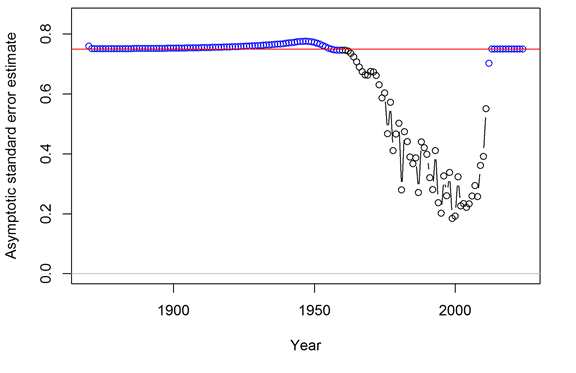
\includegraphics{appendixA_asymerror}\\
	\caption{ Timeseries of standard error estimates for the log recruitment deviations for darkblotched rockfish with 95\% uncertainty intervals. As in Figure \ref{fig:recdevs}, the black color indicates the main recruitment period. This period with lower standard error is associated with higher variability among deviations (Figure \ref{fig:recdevs}). The red line at 0.75 indicates the  $\sigma_R$ value in this model.}
	\label{fig:recSE}
\end{figure}


\begin{figure}[h]
	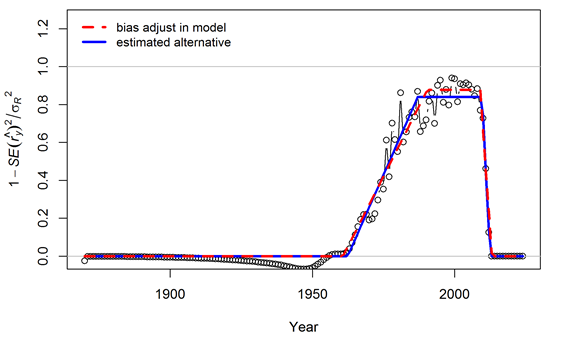
\includegraphics{appendixA_biasadj}\\
	\caption{ Transformation of the standard error estimates (shown in Figure \ref{fig:recSE}) for darkblotched rockfish following the approach suggested by \citet{methot_adjusting_2011}. These values were used to set the 5 values controlling the degree of bias adjustment (as a fraction of  $\sigma_R/2$) to account for differences in the mean and median of the lognormal distribution from which the recruitment deviations are drawn. The red line indicates a bias adjustment of 0 up to the  1960.75, ramping up to a maximum adjustment level of 0.877 for the period 1990.4–2008.98,and reducing back to 0 starting in 2013.08. Note that these values controlling the bias adjustment need not be integer year values. Also the break points in the bias adjustment function need not match the break points between early, main, and late/forecast recruitment deviation vectors (indicated by blue and black colors in Figures \ref{fig:recdevs} and \ref{fig:recSE}). The blue line indicates a functional form that minimizes the sum of squared differences between the bias adjustment function and the transformed standard error values. The subtle differences between red and blue lines are unlikely to have any appreciable effect on the model results.}
	\label{fig:ramp}
\end{figure}


\begin{figure}[h]
	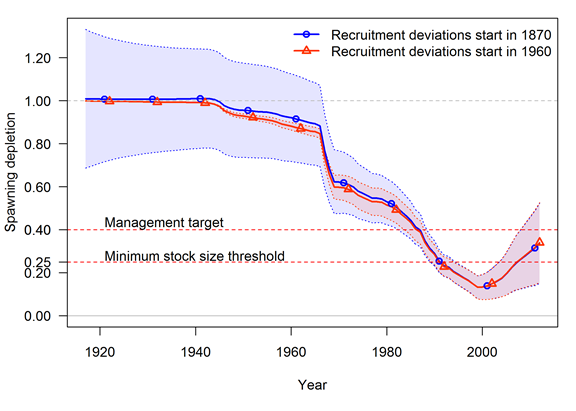
\includegraphics{appendixA_depl}\\
	\caption{ Comparison of timeseries of spawning depletion for darkblotched rockfish models with early recruitment deviations (starting in 1870) and without early deviations (only main recruitment deviations starting in 1960). The point estimates are similar, but the 95\% uncertainty intervals are substantially different. With no recruitment deviations for the early period, the estimates of spawning depletion in the early years are very precise and uncertainty increases as the stock moves into the data rich period. In contrast, the addition of the early recruitment deviations results in a large uncertainty in spawning depletion for the early years and an increase in precision as the stock moves into the data rich period. In this application, the uncertainty associated with the recent years is independent of the assumptions about early recruitments.}
\end{figure}

\myparagraph{Issues with Including Environmental Effects}
The expected level of recruitment is a function of spawning biomass, an environmental time series, and a log-bias adjustment.
\begin{equation}
	E(Recruitment) = f(SpBio) * exp(\beta*envdata) * exp(-0.5*\sigma_R^2)
\end{equation}
$\sigma_R$ is the variability of the deviations, so it is in addition to the variance "created" by the environmental effect.  So, as more of the total recruitment variability is explained by the environmental effect, the residual $\sigma_R$ should be decreased.  The model does not do this automatically.

The environmental effect is inherently lognormal.  So when an environmental effect is included in the model, the arithmetic mean recruitment level will be increased above the level predicted by f(SpBio) alone.  The consequences of this have not yet been thoroughly investigated, but there probably should be another bias correction based on the variability of the environmental data as scaled by the estimated linkage parameter, $\beta$.  It is also problematic that the environmental effect time series used as input is assumed to be measured without error.

The preferred approach to including environmental effects on recruitment is not to use the environmental effect in the direct calculation of the expected level of recruitment.  Instead, the environmental data would be used as if it was a survey observation of the recruitment deviation.  This approach is similar to using the environmental index as if it was a survey of age 0 recruitment abundance because by focusing on the fit to the deviations it removes the effect of SpBio on recruitment.  In this alternative, the $\sigma_R$ would not be changed by the environmental data; instead the environmental data would be used to explain some of the total variability represented by $\sigma_R$.  This approach may also allow greater uncertainty in forecasts, as the variability in projected recruitments would reflect both the uncertainty in the environmental observations themselves and the model fit to these observations.

\myparagraph{Initial Age Composition}
If the first year with recruitment deviations is set less than the start year of the model, then these early deviations will modify the initial age composition.  The amount of information on historical recruitment variability certainly will degrade as the model attempts to estimate deviations for older age groups in the initial equilibrium.  So the degree of bias correction is reduced linearly in proportion to age so that the correction disappears when maximum age is reached.  The initial age composition approach normally produces a result that is indistinguishable from a configuration that starts earlier in the time series and estimates a longer time series of recruitments.  However, because the initial equilibrium is calculated from a recruitment level unaffected by spawner-recruitment steepness and initial age composition adjustments are applied after the initial equilibrium is calculated, it is possible that the initial age composition approach will produce a slightly different result than if the time series was started earlier and the deviations were being applied to the recruitment levels predicted from the spawner-recruitment curve. 


\pagebreak


	%========= Section 17: Code Examples
	\section{Code Examples}
\label{sec:codeappendix}
\hypertarget{CodeEx}{}

This section provides search terms to facilitate finding code within the \href{https://github.com/nmfs-stock-synthesis/stock-synthesis}{Stock Synthesis source code}. 

\begin{itemize}
  \item Ageing Error Estimation - In \href{https://github.com/nmfs-stock-synthesis/stock-synthesis/blob/main/SS_miscfxn.tpl}{SS\_miscfxn.tpl}, search for function "get\_age\_age" or "SS\_Label\_Function 45".
  \item Survival Based SRR Code - In \href{https://github.com/nmfs-stock-synthesis/stock-synthesis/blob/main/SS_recruit.tpl}{SS\_recruit.tpl}, search for "SS\_Label\_43.3.7  survival based".
  \item Random Walk Selectivity: Pattern 17 - In \href{https://github.com/nmfs-stock-synthesis/stock-synthesis/blob/main/SS_selex.tpl}{SS\_selex.tpl}, search for "SS\_Label\_Info\_22.7.17".
  \item Cubic Spline Selectivity - In \href{https://github.com/nmfs-stock-synthesis/stock-synthesis/blob/main/SS_selex.tpl}{SS\_selex.tpl}, search for "SS\_Label\_Info\_22.7.27".
  \item Deviation Link - In \href{https://github.com/nmfs-stock-synthesis/stock-synthesis/blob/main/SS_timevaryparm.tpl}{SS\_timevaryparm.tpl}, search for "SS\_Label\_Info\_14.3".\
\end{itemize}

\normalfont % this sets the main font to crimson
\normalsize %% return the text to 12 point font - otherwise you end up with 22 point font!

\pagebreak	
	%========= Section 18: Change Log
	% S
\section{Change Log}

This section has been removed from the user manual. Information on changes to SS is now recorded in the change log spreadsheet available on VLAB (vlab.ncep.noaa.gov/group/stock-synthesis/home). Fields include version number, date, type (e.g. new, clarify, fix), and category (e.g. growth, selectivity).

\pagebreak

%=========New SS 3.30 Features and Detected Issues
\section{New Features Available in Stock Synthesis Version 3.30}

Stock Synthesis version v.3.30 was designed specifically to provide more precise control in modeling temporal changes in biology, expected values for data, and for recruitment.  In addition, a large number of new features that make substantial changes to the input formats have been introduced.  Two executables of SS are provided.  One, ss\_trans.exe, will read SS v.3.24 input files and produce SS v.3.30 formatted versions of those input files.  Nearly every feature in SS v.3.24 can be converted by this program.  The other executable, ss.exe, is the primary new assessment tool. Additional information on each new feature is available by clicking on the item.

		
\begin{center}
	{\renewcommand{\arraystretch}{1.5}%
	\begin{longtable}{p{1.75cm} p{9.5cm}}
		\hline
		Item &  Description\\
		\hline
		\endfirsthead
		\hline
		\toprule
		Item &  Description\\
		\hline
		\endhead

		\hline
		\endfoot

		\endlastfoot
		
		\multicolumn{1}{l}{\hyperlink{GenericFleets}{Generic Fleets}} & 
				Fleet specification section of data file has substantially changed and now includes specific fleet type; fishery fleets, bycatch fleets, and surveys which can be specified in any order.\\

		\multicolumn{1}{l}{\hyperlink{ListBased}{List-oriented inputs}} & 
			    Older versions of SS (3.24 and earlier) required users to specify the number of items to be read, now SS can determine the number of lines to read through the application of a terminator line using -9999 in first field of the read vector. \\
		  
		\multicolumn{1}{l}{\hyperlink{SubSeas}{Internal sub-seasons}} & 
			    SS v.3.24 inherently has 2 subseasons within each season (begin and middle) at which the age-length-key is calculated; now user specifies an even number of sub-seasons to use (2 to many). \\

		\multicolumn{1}{l}{\hyperlink{ObsTiming}{Observation Timing}} & 
			    Timing of observations now is input as year and month (e.g., April 15 is 4.5). The age-length-key used for each observation is calculated to the nearest sub-season month.  Old "survey\_timing" replaced by the month specific inputs.  Season is calculated at runtime from the input month and the input season durations. \\

		\multicolumn{1}{l}{\hyperlink{ALK}{Speed}} & 
			    Smarter at when to re-calculate the age-length-key; trims tails of size-at-age so calculations avoid many inconsequential cells of the age-length matrix. Age-length-key tail compression is specified in the starter file.\\
		
		\multicolumn{1}{l}{\hyperlink{Convert} {Converter}} & 
			    Special version of SS, ss\_trans.exe, will read files in SS v.3.24 format and write *.ss\_new files in SS v.3.30 format.  This is the advised method for converting previous version files, but always do a side-by-side comparison.\\

		\multicolumn{1}{l}{\hyperlink{WAAparm} {Weight-at-Age}} & Implementing empirical weight-at-age is now specified separately in the control file rather than under the maturity options.\\

		\multicolumn{1}{l}{\hyperlink{Priors}{Prior Type}} & Change in the prior numbering for parameters.  Now, 0 indicates no prior, and 6 indicates a normal distribution prior.\\
		
		\multicolumn{1}{l}{\hyperlink{CatchMult}{Catch multiplier}} & 
				Each fishing fleet's catch can now have a catchability (Q) that is a parameter in the mortality-growth parameter section.\\
				
		\multicolumn{1}{l}{\hyperlink{CatchFormat}{Catch input}} & 
				Catch input now as list:  year, season, fleet, amount, standard error. \\
				
		\multicolumn{1}{l}{\hyperlink{CompTiming}{Observations}} & 
				Fishery composition observations can be related to season long catch-at-age, or to a month-specific timing.\\
		
		\multicolumn{1}{l}{\hyperlink{DomeRetention}{Retention}} & 
				Option for dome-shaped retention function and for age-based retention. \\

		\multicolumn{1}{l}{Scaling Options} & 	
				New non-parametric selectivity types that are scaled by the raw values at particular ages, rather than the max age.\\
		\multicolumn{1}{l}{\hyperlink{2DAR}{2D AR Selectivity}} &
				Implementation of two-dimensional autoregressive selectivity implemented in SS v.3.30.10.\\

		\multicolumn{1}{l}{\hyperlink{SpecialSurvey}{Special survey types}} & 
				Special selectivity options (type 30 or $>$) are no longer specified within the control file.  Specifying the use of one of these selectivity types is now done within the data file by selecting the survey "units". \\  

		\multicolumn{1}{l}{\hyperlink{Qsetup}{Link functions}} & 
				Q\_power is now one of several, and growing, set of link functions for catchability. \\
				
		\multicolumn{1}{l}{\hyperlink{Qsetup}{Catchability setup}} & 
				Major reorganization of catchability (Q) setup, including the link specification. \\
			
		\multicolumn{1}{l}{\hyperlink{Qsetup}{Q as a parameter}} & 
				Each survey now must have a Q parameter and its value still can float (as old option 5).\\

		\multicolumn{1}{l}{\hyperlink{Shepherd}{Shepherd SRR}} & 
				The traditional 3-parameter Shepherd stock-recruitment curve is now an option.\\

%		\multicolumn{1}{l}{\hyperlink{Shepherd2}{Shepherd SRR re-parameterization}} & 
%				A re-parameterized 3-parameter Shepherd stock-recruitment curve, distinct from the traditional parameterization, is now an option in SS v.3.30.11 and higher.\\
			
		\multicolumn{1}{l}{\hyperlink{Ricker2}{Ricker SRR}} & 
				A 3-parameter Ricker stock-recruitment curve is now an option in SS v.3.30.11 and higher.\\

		\multicolumn{1}{l}{\hyperlink{RecrTiming}{Recruitment timing}} & 
				Replace "birthseason" with "settlement event" that has explicit timing offset from spawning. Month of spawning and each settlement event must be specified and need not be at beginning of a season.\\

		\multicolumn{1}{l}{Global MSY} &  
				Global MSY based on knife-edged age selection; also do calculation with single age selection. The global MSY value will automatically be included in the report file.\\
		
		\multicolumn{1}{l}{ Mean recruitment distribution} & 
				In multi-area model, can now specify range of years to use for the average recruitment distribution for forecasting. This feature is not yet implemented. \\

		\multicolumn{1}{l}{Process error} & 
				Propagate random walk in mortality growth parameters, catchability, and selectivity into forecast. Specifying the end year for process error in the forecast period will implement this option.  This option has only been partial implemented at this junction and will be completed in later versions.\\

		\multicolumn{1}{l}{\hyperlink{MGorder}{Parameter order}} & 
				Mortality growth parameters now have maturity, fecundity, sex ratio, and weight-length by growth pattern.\\
				
		\multicolumn{1}{l}{\hyperlink{SexRatio}{Sex ratio}} & 
			    Change sex ratio at birth from a constant to a morph-specific mortality growth parameter. This feature was not correctly implemented in SS v.3.30 earlier than v.3.30.12. \\

		\multicolumn{1}{l}{\hyperlink{GrowthCessation}{Growth cessation}} & 
		    New growth option which allows for growth cessation, implemented in SS v.3.30.13. \\

		\multicolumn{1}{l}{\hyperlink{GcompVar}{Input variance adjuster}} & 
				Added variance adjustment factor for generalized size comp. \\
			
		\multicolumn{1}{l}{Deviation vectors} & 
				Variance of deviation vectors is now specified with 2 parameters for standard error and auto-correlation (rho), so can be estimated.\\
				
		\multicolumn{1}{l}{\hyperlink{Dirichlet}{Dirichlet multinomial}} & 
				Dirichlet multinomial now a fleet-specific option; takes one parameter per fleet. \\

		\multicolumn{1}{l}{\hyperlink{paraOrder}{Parameter order}} & The prior standard deviation column for all parameter lines has been moved before the prior type column.  This modification improves formatting output between integer and decimal inputs.\\ 

		\multicolumn{1}{l}{Density dependence} & 
				Beginning of year summary biomass and the recruitment deviation parameters are mapped to the "environmental" matrix so that parameters can be density-dependent based on environmental factors.\\
				
		\multicolumn{1}{l}{\hyperlink{tvOrder}{Re-order}} & 
				Pay attention to the new order of the time-varying adjustments to parameters (block/trend, then environmental, then deviations). \\
			
		\multicolumn{1}{l}{\hyperlink{time-vary}{Time-varying parameters}} & 
				Long parameter lines for spawner-recruit relationship (SRR), catchability (Q), and tag parameters and complete re-vamp of the way that time-varying parameters are implemented for SRR and Q.  Now shares same internal code as mortality-growth and selectivity parameters for time-varying capabilities.\\

		\multicolumn{1}{l}{Version numbering}	& The implementation of as new version control has changed how executable versions will be specified. The executable releases are now named SS3.3x.xx.xx representing, in order; major features, minor features, and code fixes. \\
		 \hline
	\end{longtable}}
\end{center}


\subsection{SS v.3.24 Issues Detected}
The process of updating and adding new features within SS v.3.30 exposed several issues with the previous version that have been corrected:
\begin{enumerate}
	\item Recruitment timing in multi-season models: When spawning occurred in a late season one year and recruits occurred at beginning of a season the next year, the recruits were starting at age-0, which was illogical.  SS v.3.30 corrects this so that recruits are age-0 only if recruiting at or between the time of spawning and the end of the year, and recruits after January 1st start at age-0.  A manual option in the control file allows users to attempt to replicate the SS v.3.24 protocol.
	
	\item Lorenzen $M$ and time-varying growth interaction: There needs to be a revision to SS v.3.30 so that growth can be updated each season prior to calculating Lorenzen $M$.
	
	\item Length at maximum age: SS v.3.24 intended to decay numbers at the maximum length over-time at $M + F$ decreasing the abundance of fish implicitly older than the maximum age (agemax).  However, this decay was only implemented in years for which time-varying growth was updated. 
	 
	\item SS v.3.24 had a lower bound of 1 when adjusting annual sample size (Nsamp) downward for composition data (length and age).  The variance adjustment factors specified in the control file are multiplied across all annual sample size values for each data source (fleet and composition type).  The issue with the lower bound of 1 resulted in sample size adjustment not being constant across small and large sample size years, possibly resulting in smaller samples have higher impact than may be desired.  SS v3.30 has reduced this lower bound to a value of 0.001 but has retained user control over this value within the data file ("minsamplesize" column in the Composition Data Structure matrix at the top of the length and age data sections) to allow comparison with older model versions. 
\end{enumerate}	
	%========= Reference Section
	\newpage
	\bibliography{SS}
	\bibliographystyle{JournalBiblio/cjfas}
	\newpage	
		
	% Appendices ===================================
	%========= Section 17: Appendix A: Recruitment 
	%\section{Appendix A: Recruitment Variability and Bias \\ Correction }


Recruitments in SS are defined as lognormal deviates around a log-bias adjusted spawner- recruitment curve.  The magnitude of the log-bias adjustment is calculated from the level of $\sigma_R$ , which is the standard deviation of the recruitment deviations (in log-space).  There are 5 segments of the time series in which to consider the effect of the log-bias adjustment: virgin; initial equilibrium; early data-poor period; data-rich period; very-recent/forecast. The choice of break points between these segments need not correspond directly with the settings for the bias adjustment, although some alignment might be desired. Methot and Taylor (2011) provide more detailed discussion of the bias adjustment than what is provided below but do not address the separation of time periods into separate segments. The approach is illustrated with figures associated with a recent assessment for darkblotched rockfish (Gertseva and Thorson, 2013).

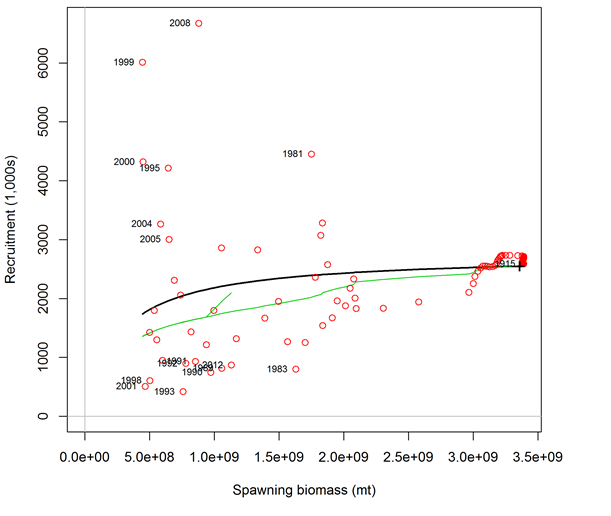
\includegraphics{appendixA_recruits}\\
\figurename{ A.1. Spawner-recruitment relationship for darkblotched rockfish (Gertseva and Thorson, 2013). Red points represent estimated recruitments, the solid black line is the stock-recruit relationship and the green line represents the adjustment to this relationship after adjustment to account for the lognormal distribution associated with each year. The “+” symbol labeled 1915 near the right side represents both the virgin and initial equilibrium of the model. The numerous red points close to the initial conditions correspond to the early years of the model with low harvest rates.}

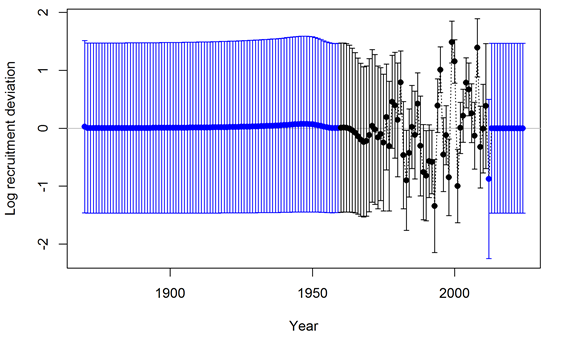
\includegraphics{appendixA_logdevs}\\
\figurename{ A.2. Timeseries of log recruitment deviations for darkblotched rockfish with 95\% uncertainty intervals. The start year of the model is 1915, but recruitment deviations are estimates starting in 1870. The 45 deviation estimates for 1870–1914 inform the age structure used in the start year. The black color for the years 1960–2011 indicates the “main” recruitment deviation vector, while the blue color for the years 1870–1959 and 2012–2024 indicates the “early” and “late/forecast” recruitment deviation vectors, respectively. }

\begin{description}
	\item[Virgin]\hfil\\
	The R0 level of recruitment is a parameter of the spawner-recruitment curve.  This recruitment and the corresponding spawning biomass, S0, are expected to represent the long-term arithmetic mean.
	\item[Initial Equilibrium]\hfil\\
	The level of recruitment is typically maintained at the R0 level even though the initial equilibrium catch will reduce the spawning biomass below the virgin level.  If steepness is moderately low or the initial F is high, then the lack of response in recruitment level may appear paradoxical.  The logic is that building in the spawner-recruitment response to initial F would significantly complicate the calculations and would imply that the initial equilibrium catch level had been going on for multiple generations.  If the lack of response is considered to be problematic in a particular application, then start the model at an earlier year and with a lower initial equilibrium catch so that the dynamics of the spawner-recruitment response get captured in the early period, rather than getting lost in the initial equilibrium.
	\item[Early data-poor period]\hfil\\
	This is the early part of the time series where the only data typically are landed catch.  There are no data to inform the model about the specific year-to-year fluctuations in recruitment, although the ending years of this period will begin to be influenced by the data.  The “early time period” is not a formal concept. 	It is up to the user to decide whether to start estimating recruitment deviations beginning with the first year of the model, or to delay such estimation until the data become more informative. Modeling recruitment deviations in this period may lead to a more realistic portrayal of the uncertainty in depletion, but can also lead to spurious patterns in estimated recruitments that may be driven by the fit to index data or other sources that would not be expected to have accurate information on recruitment.
	\begin{itemize}
		\item Option A: Do not estimate recruitment deviations during this early period.  During years prior to the first year of recruitment deviations, the model will set the recruitment equal to the level of the spawner-recruitment curve.  Thus, it is a mean-based level of recruitment.  Because these annual parameters are fixed to the level of the spawner-recruitment curve, they have no additional uncertainty and make no contribution to the variance of the model. This approach may produce relatively large, or small, magnitude deviations at the very beginning of the subsequent period, as the model “catches up” to any slight signal that could not be captured through estimated deviations in the early data-poor period.  There may be some effect on the estimate of R0 as a result of lack of model flexibility in balancing early period removals with signal in the early portion of the data-rich period.  
		\item Option B: Estimate recruitment deviations for all the early years.  Each of these recruitment deviations is now a dev parameter so will have a variance that contributes to the total model variance.  The estimated standard deviation of each of these dev parameters should be similar to $\sigma_R$ because $\sigma_R$ is the only constraint on these parameters (however, the last few in the sequence will begin to feel the effect of the data so may have lower standard deviations). 		
	\end{itemize}
	\item[Data-rich period]\hfil\\
	Here the data inform the model on the year-to-year level of recruitment.  These fluctuations in recruitment are assumed to have a lognormal distribution around the log-bias adjusted spawner-recruitment curve.  The level of $\sigma_R$ input to the model should match this level of fluctuation to a reasonable degree.  Because the recruitments are lognormal, they produce a mean biomass level that is comparable to the virgin biomass and thus the depletion level can be calculated without bias.  However, if the early period has recruitment deviations estimated by MPD, then the depletion levels during the early part of the data-rich period may have some lingering effect of negative bias during the early time period. The level of $\sigma_R$ should be at least as large as the level of variability in these estimated recruitments.  If too high a level of $\sigma_R$ is used, then a bias can occur in the estimate of spawner-recruitment steepness, which determines the trend in recruitment.  This occurs when the early recruitments are taken directly from the spawner-recruitment curve, so are mean unbiased, then the later recruitments are estimated as deviations from the log-bias adjusted curve.  If $\sigma_R$ is too large, then the bias-adjustment is too large, and the model may compensate by increasing steepness to keep the mean level of recent recruitments at the correct level.
	\item[Recent Years/Forecast]\hfil\\
	Here the situation is very similar to the early time period in that there are no data to inform the model about the year-to-year pattern in recruitment fluctuations so all devs will be pulled to a zero level in the MPD.  The structure of SS creates no sharp dividing line between the estimation period and the forecast period.  In many cases one or more recruitments at the end of the time series will lack appreciable signal in the data and should therefore be treated as forecast recruit deviations.  To the degree that some variability is observed in these recruitments, partial or full bias correction may be desirable for these devs separate from the purely forecast devs, there is therefore an additional control for the level of bias correction applied to forecast deviations occurring prior to endyear+1.
\end{description}

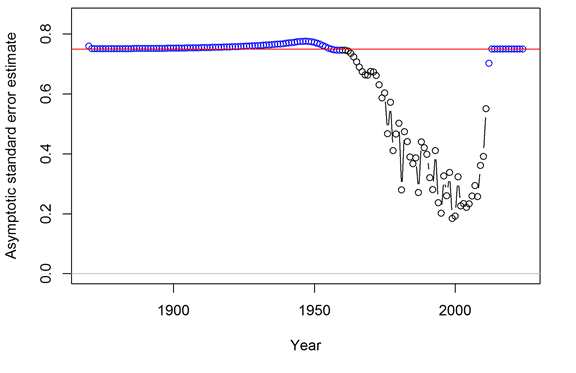
\includegraphics{appendixA_asymerror}\\
\figurename{ A.3. Timeseries of standard error estimates for the log recruitment deviations for darkblotched rockfish with 95\% uncertainty intervals. As in Figure A.2, the black color indicates the main recruitment period. This period with lower standard error is associated with higher variability among deviations (Figure A.2). The red line at 0.75 indicates the  $\sigma_R$ value in this model.}

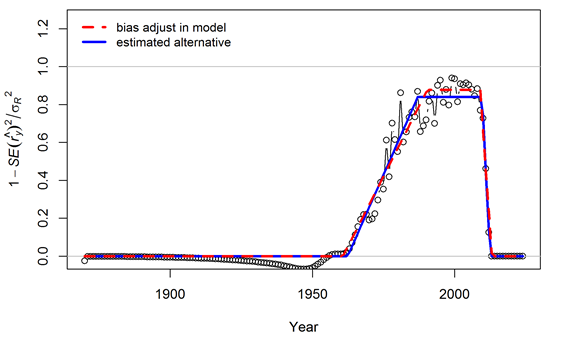
\includegraphics{appendixA_biasadj}\\
\figurename{ A.4. Transformation of the standard error estimates (shown in Figure A.3) for darkblotched rockfish following the approach suggested by Methot and Taylor (2011). These values were used to set the 5 values controlling the degree of bias adjustment (as a fraction of  $\sigma_R/2$) to account for differences in the mean and median of the lognormal distribution from which the recruitment deviations are drawn. The red line indicates a bias adjustment of 0 up to the  1960.75, ramping up to a maximum adjustment level of 0.877 for the period 1990.4–2008.98,and reducing back to 0 starting in 2013.08. Note that these values controlling the bias adjustment need not be integer year values. Also the break points in the bias adjustment function need not match the break points between early, main, and late/forecast recruitment deviation vectors (indicated by blue and black colors in Figures A.2 and A.3). The blue line indicates a functional form that minimizes the sum of squared differences between the bias adjustment function and the transformed standard error values. The subtle differences between red and blue lines are unlikely to have any appreciable effect on the model results.}

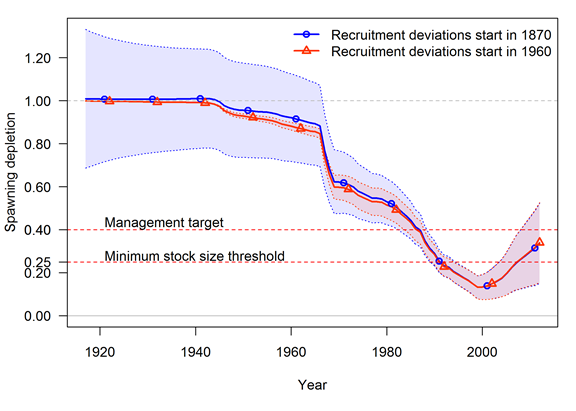
\includegraphics{appendixA_depl}\\
\figurename{ A.5. Comparison of timeseries of spawning depletion for darkblotched rockfish models with early recruitment deviations (starting in 1870) and without early deviations (only main recruitment deviations starting in 1960). The point estimates are similar, but the 95\% uncertainty intervals are substantially different. With no recruitment deviations for the early period, the estimates of spawning depletion in the early years are very precise and uncertainty increases as the stock moves into the data rich period. In contrast, the addition of the early recruitment deviations results in a large uncertainty in spawning depletion for the early years and an increase in precision as the stock moves into the data rich period. In this application, the uncertainty associated with the recent years is independent of the assumptions about early recruitments.}

\subsection{Issues with Including Environmental Effects}
The expected level of recruitment is a function of spawning biomass, an environmental time series, and a log-bias adjustment.
\begin{equation}
	E(Recruitment) = f(SpBio) * exp(\beta*envdata) * exp(-0.5*\sigma_R^2)
\end{equation}
$\sigma_R$ is the variability of the deviations, so it is in addition to the variance “created” by the environmental effect.  So, as more of the total recruitment variability is explained by the environmental effect, the residual $\sigma_R$ should be decreased.  The model does not do this automatically.

The environmental effect is inherently lognormal.  So when an environmental effect is included in the model, the arithmetic mean recruitment level will be increased above the level predicted by f(SpBio) alone.  The consequences of this have not yet been thoroughly investigated, but there probably should be another bias correction based on the variability of the environmental data as scaled by the estimated linkage parameter, $\beta$.  It is also problematic that the environmental effect time series used as input is assumed to be measured without error.

The preferred approach to including environmental effects on recruitment is not to use the environmental effect in the direct calculation of the expected level of recruitment.  Instead, the environmental data would be used as if it was a survey observation of the recruitment deviation.  This approach is similar to using the environmental index as if it was a survey of age 0 recruitment abundance because by focusing on the fit to the deviations it removes the effect of SpBio on recruitment.  In this alternative, the $\sigma_R$ would not be changed by the environmental data; instead the environmental data would be used to explain some of the total variability represented by $\sigma_R$.  This approach may also allow greater uncertainty in forecasts, as the variability in projected recruitments would reflect both the uncertainty in the environmental observations themselves and the model fit to these observations.

\subsection{Initial Age Composition}
If the first year with recruitment deviations is set less than the start year of the model, then these early deviations will modify the initial age composition.  The amount of information on historical recruitment variability certainly will degrade as the model attempts to estimate deviations for older age groups in the initial equilibrium.  So the degree of bias correction is reduced linearly in proportion to age so that the correction disappears when maximum age is reached.  The initial age composition approach normally produces a result that is indistinguishable from a configuration that starts earlier in the time series and estimates a longer time series of recruitments.  However, because the initial equilibrium is calculated from a recruitment level unaffected by spawner-recruitment steepness and initial age composition adjustments are applied after the initial equilibrium is calculated, it is possible that the initial age composition approach will produce a slightly different result than if the time series was started earlier and the deviations were being applied to the recruitment levels predicted from the spawner-recruitment curve. 
	
	%========= Section 18: Appendix B: Data Weighting
	%\section{Appendix B: Data Weighting }
\begin{sloppypar}
In 2015 there was a CAPAM workshop dedicated to data-weighting. Description of the workshop can be found at http://www.capamresearch.org/data-weighting/workshop. The presentations from the workshop are available through that website and many of them were included in a special issue of Fisheries Research a https://www.sciencedirect.com/journal/fisheries-research/vol/192.
\end{sloppypar}

Currently, there are three main methods for weighting length and data applied for U.S. West Coast assessments using Stock Synthesis.

\begin{enumerate}
	\item \textbf{McAllister - Ianelli}: Effective sample size is calculated from fit of observed to expected length or age compositions. Tuning algorithm is intended to make the arithmetic mean of the input sample size equal to the harmonic mean of the effective sample size \citep{mcallister_bayesian_1997}.
	
	\item \textbf{Francis}: Based on variability in the observed mean length or age by year, where the sample sizes are adjusted such that the fit of the expected mean length or age should fit within the uncertainty intervals at a rate which is consistent with variability expected based on the adjusted sample sizes (Method "TA1.8") \citep{francis_data_2011}
	
	\item \textbf{Dirichlet-Multinomial}: A new likelihood (as opposed to the standard multinomial) which includes an estimable parameter (theta) which scales the input sample size. In this case, the term "Effective sample size" has a different interpretation than in the McAllister-Ianelli approach \citep{thorson_model-based_2017}.
\end{enumerate}

\subsection{Applying the methods}

\subsubsection{McAllister-Ianelli}
The "Length\_Comp\_Fit\_Summary" and "Age\_Comp\_Fit\_Summary" sections in the Report file include information on the harmonic mean of the effective sample size and arithmetic mean of the input sample size used in this tuning method. In the r4ss package, these tables are returned by the \texttt{SS\_output} function as \texttt{ \$Length\_comp\_Eff\_N\_tuning\_check} and \texttt{ \$Age\_comp\_Eff\_N\_tuning\_check}.

A convenient way to process these values into the format required by the control file is to use the function:

\texttt{ SS\_tune\_comps(replist, option = "MI") }

where the input "replist" is the object created by \texttt{SS\_output}. This function will return a table and also write a matching file called "suggested\_tuning.ss" to the directory where the model was run.

For models using SS version 3.30, the table created by \texttt{SS\_tune\_comps} can be pasted into the bottom of the control file in the section labeled “Input variance adjustments”, followed by the terminator line which indicates the end of the section. Here's an example of the first few rows of the table followed by the terminator line (not added by the function):

\begin{center}
	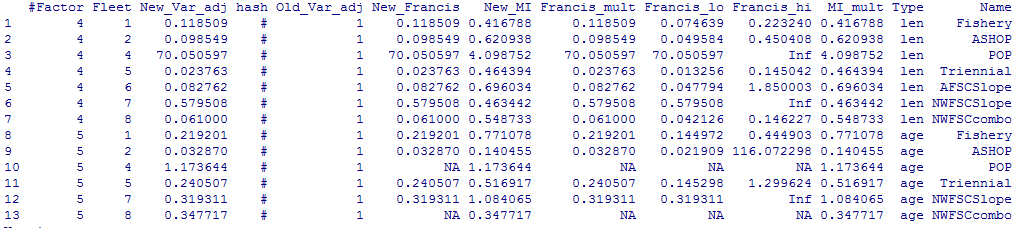
\includegraphics[scale = 0.6]{appendixB_sstune}\\
\end{center}

Also see the help page for the r4ss function \texttt{SS\_varadjust} which can be used to automatically write a new control file if you want to streamline the process of applying multiple iterations of this tuning method.

If the tuning has been implemented, the green lines in the figure below would intersect at a point which is on the black 1-to-1 diagonal line in this figure created by the r4ss function \texttt{SS\_plots}.

\begin{center}
	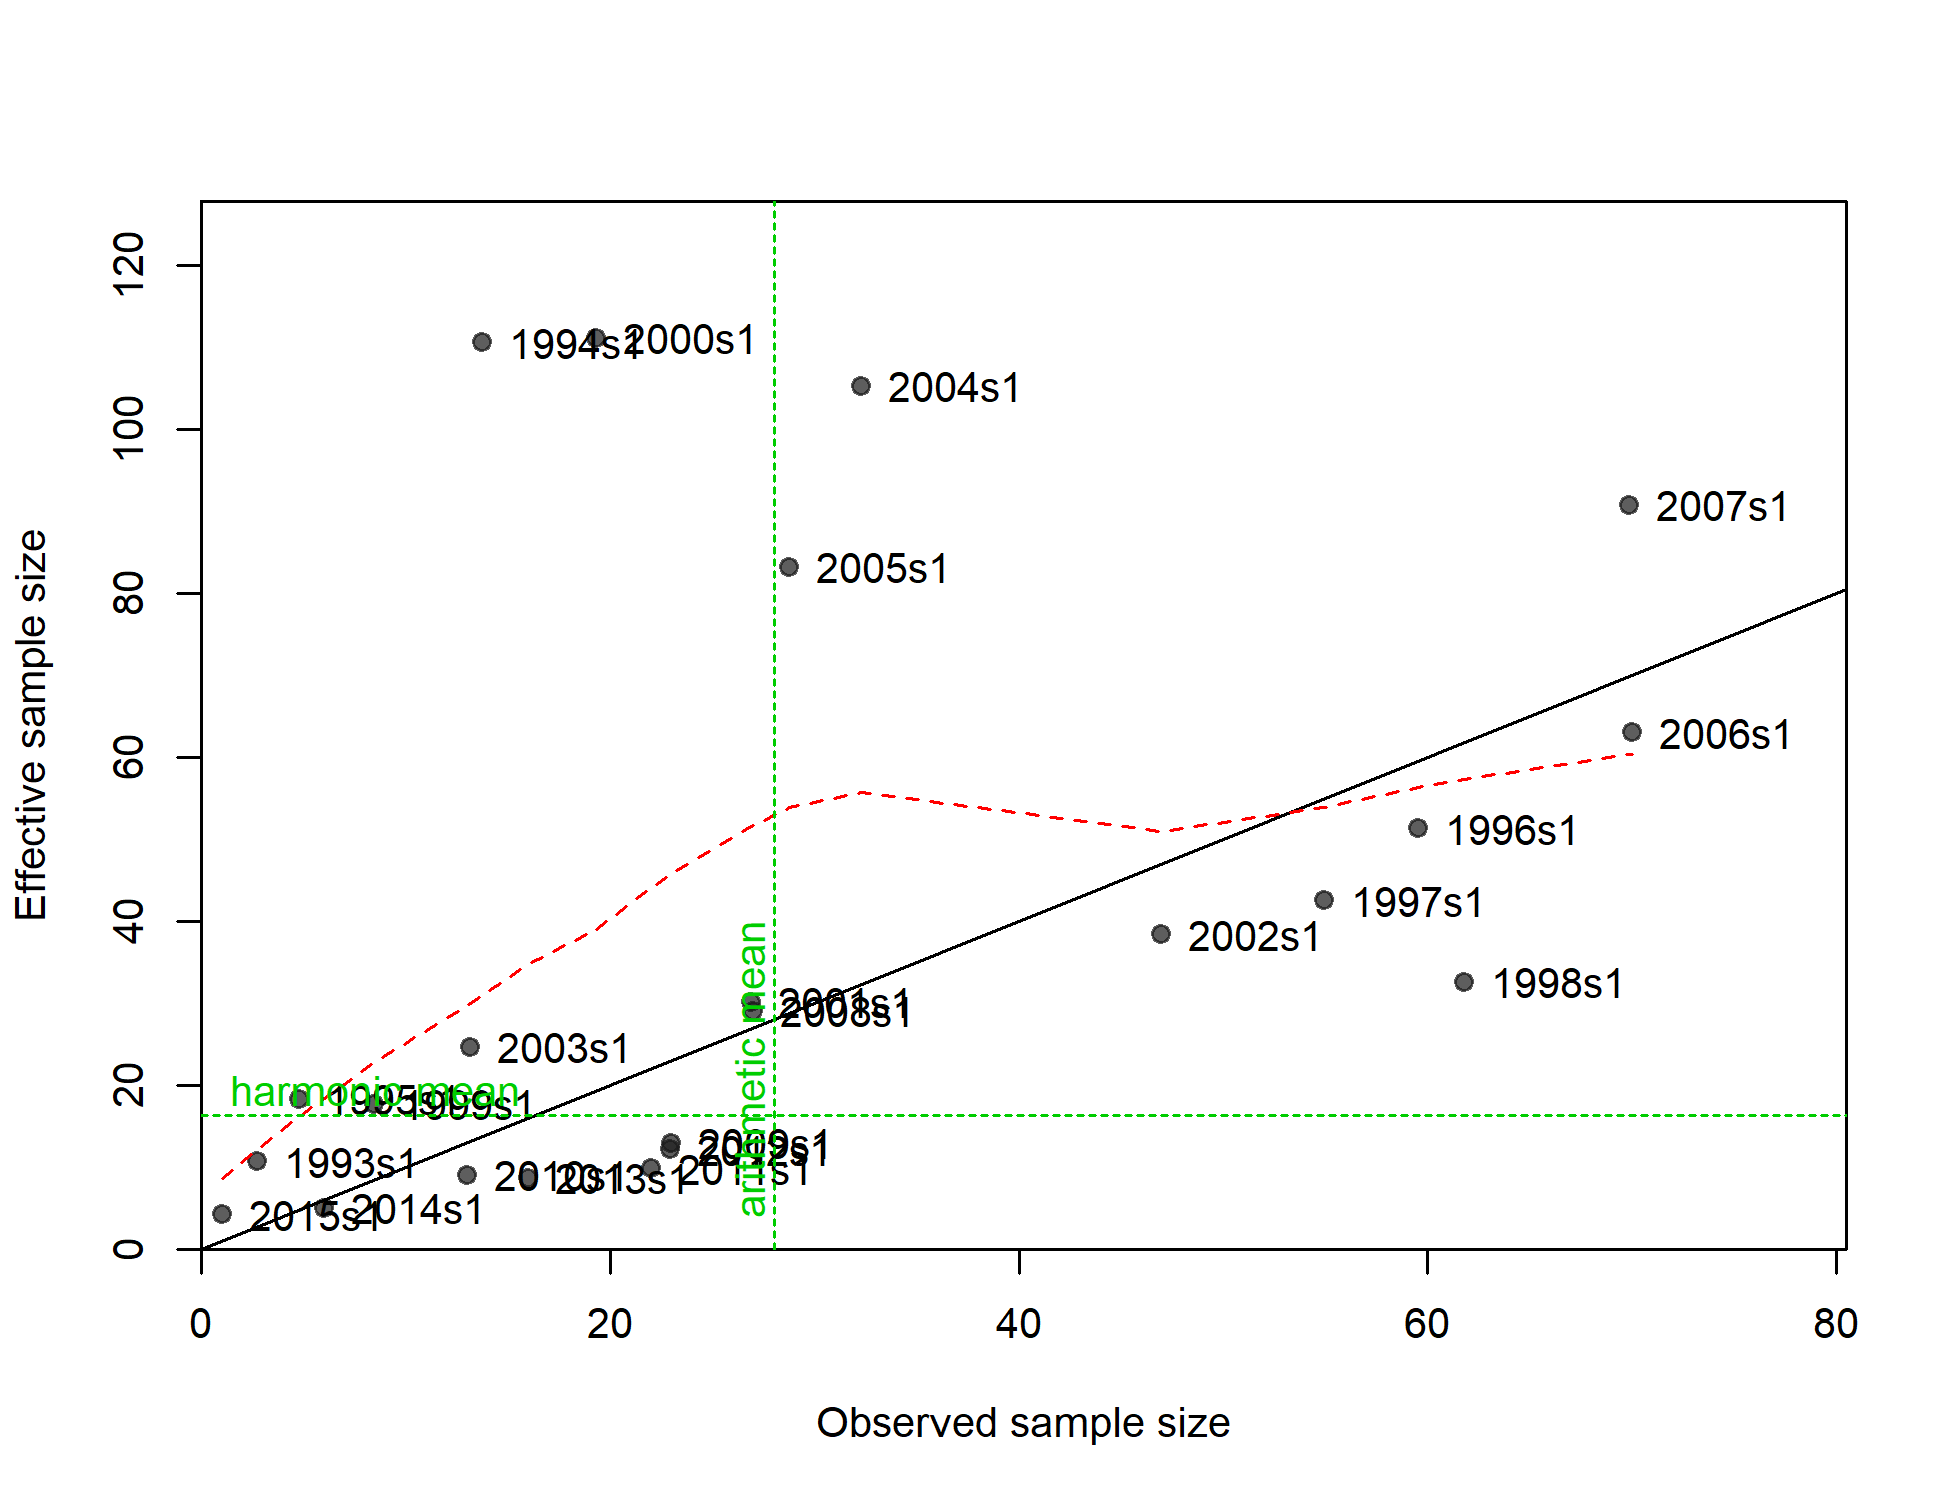
\includegraphics[scale = 0.25]{appendixB_McAllister_Ianelli}\\
\end{center}
\figurename{ B.1.N vs. EffN comparison, Length composition data as plotted by r4ss.}

There are a couple of challenges posed by the McAllister-Ianelli data-weighting approach:
\begin{enumerate}
	\item Subjective choice of how many iterations to take to achieve adequate convergence. Often just one iteration is applied.
	
	\item Takes time to implement so tuning is rarely repeated during retrospective or sensitivity analyses.
\end{enumerate}

\subsubsection{Francis}

Implementation: recommended adjustments are calculated by the r4ss functions SSMethod.TA1.8 and SSMethod.Cond.TA1.8. These functions are rarely used alone but are called by the SS\_plots function when making plots like the one below. For SS 3.30 models, the simplest way to get the adjustments in the format required by the control file is to use the \texttt{SS\_tune\_comps} function (described above under the McAllister-Ianelli method), but with a different option specified: 

\texttt{SS\_tune\_comps(replist, option = "Francis")}

The figure below shows the estimated 95\% intervals around the observed mean length by year based on the input sample size (thick lines) and the increase in that uncertainty which would occur if the sample sizes were adjusted according to the proposed multiplier.

\begin{center}
	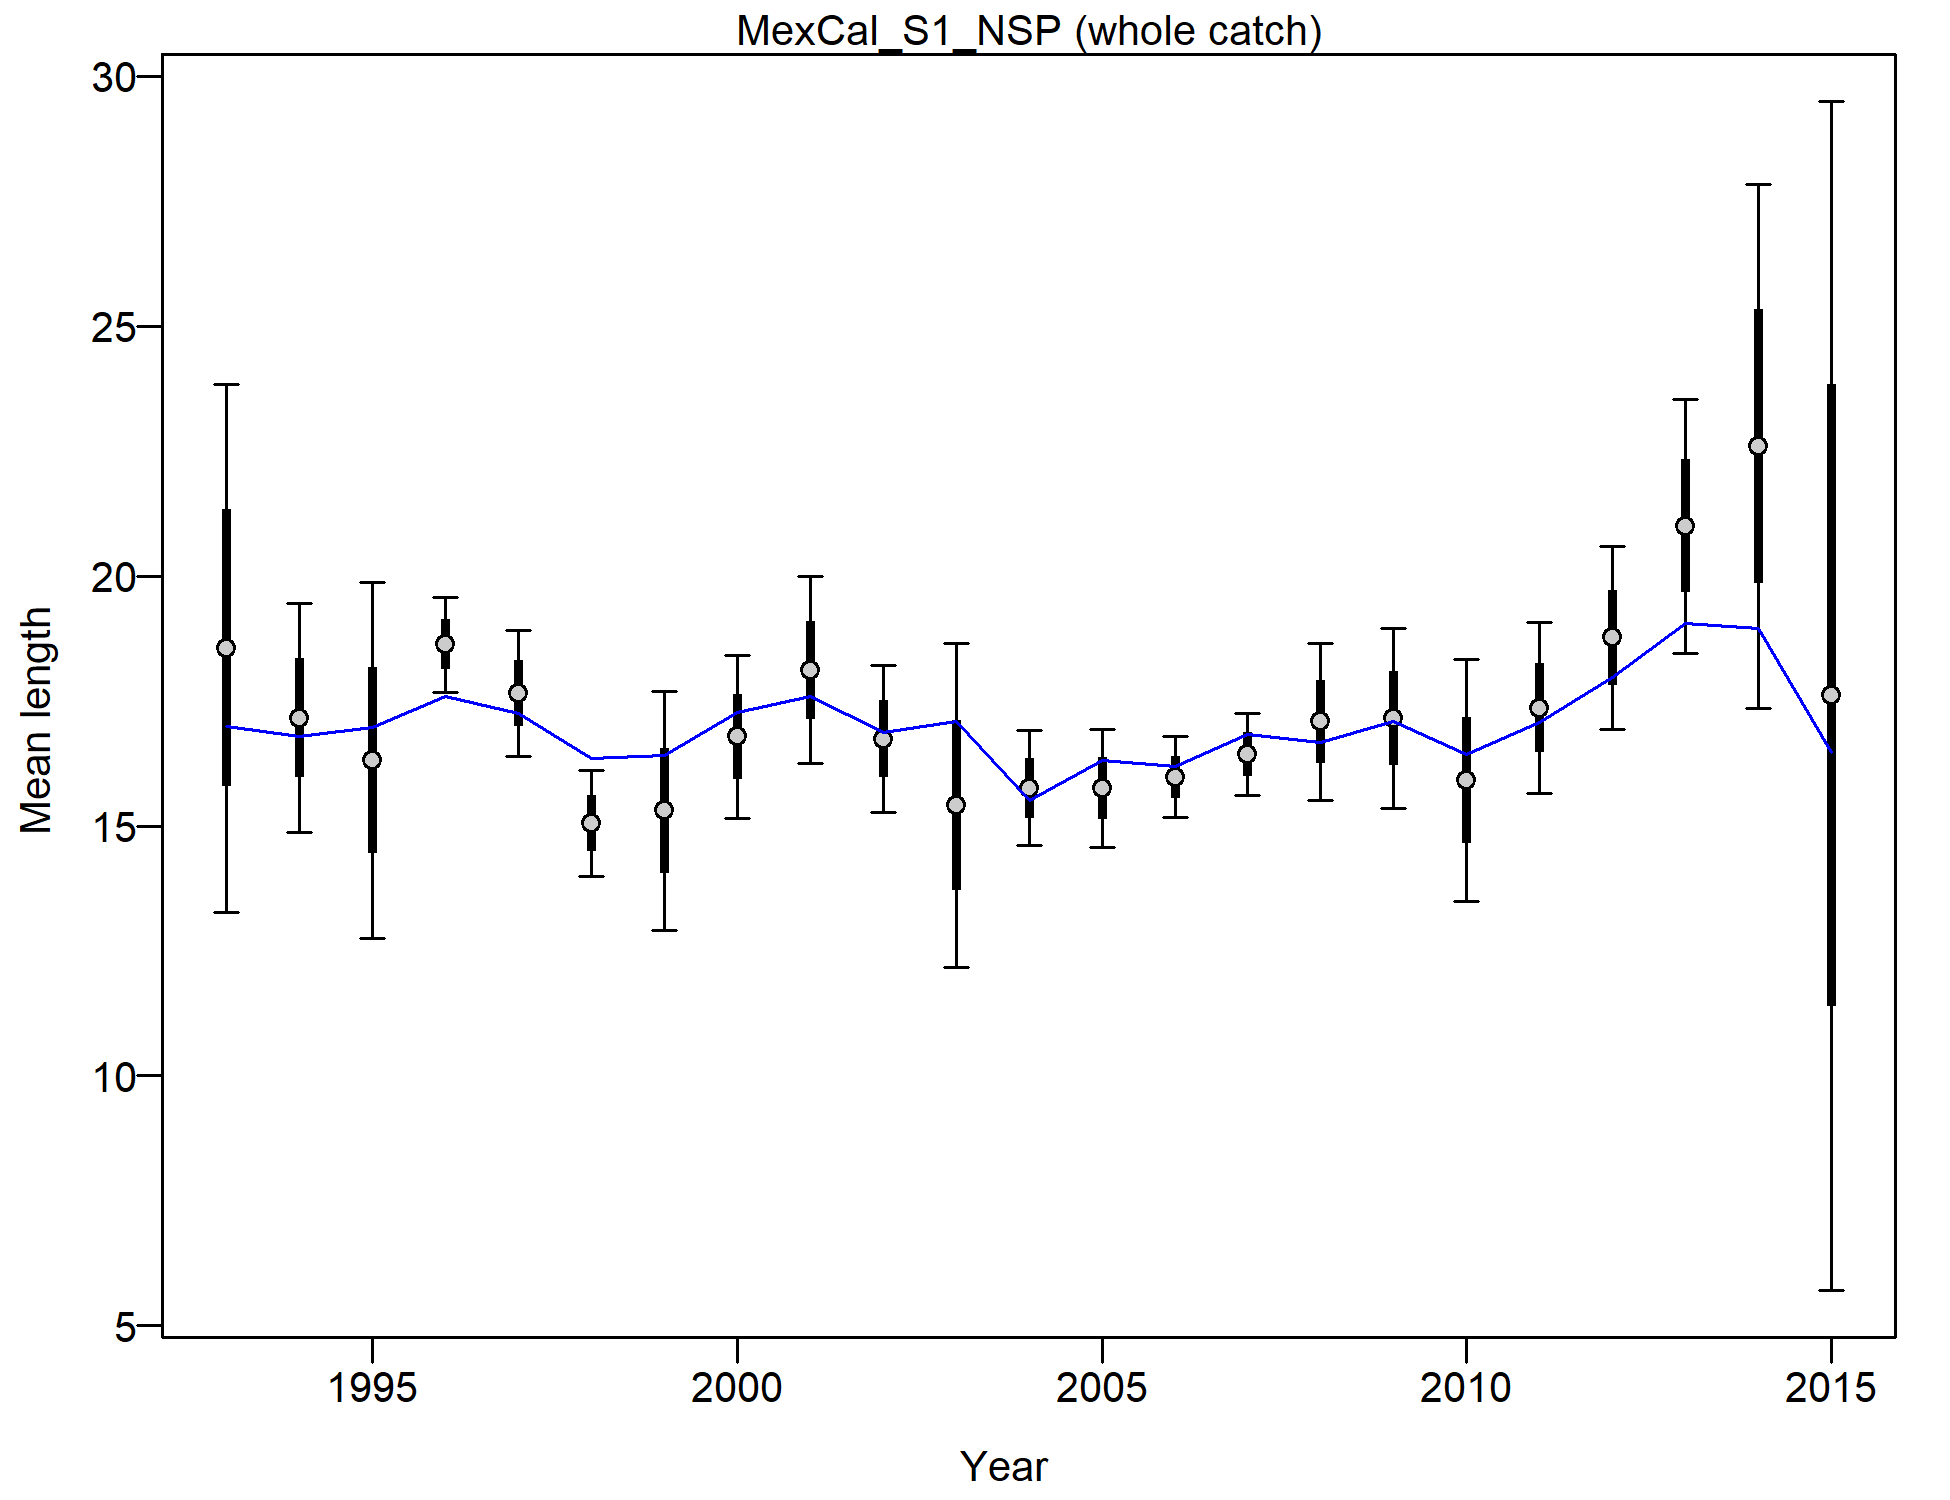
\includegraphics[scale = 0.25]{appendixB_Francis}\\
\end{center}
\figurename{ B.2.Mean length for Fleet1 with 95\% confidence intervals based on current samples sizes. Francis data weighting method TA1.8: thinner intervals (with capped ends) show result of further adjusting sample sizes based on suggested multiplier (with 95\% interval) for len data from Fleet1: 0.2739 (0.1661-0.6305)}

There are a several of challenges posed by the Francis data-weighting approach:
\begin{enumerate}
	\item Subjective choice of how many iterations to take to achieve adequate convergence. Often just one iteration is applied.
	
	\item Takes time to implement so tuning is rarely repeated during retrospective or sensitivity analyses.
	
	\item Recommended adjustment can be sensitive to outliers (remove a few years of anomalous composition data can lead to large change in recommended adjustment).
\end{enumerate}

\subsubsection{Dirichlet-Multinomial}
Change the choice of likelihood and set parameter choices in the data file:

\begin{itemize}
	\item In the specification of the length and/or age data, change "CompError" column in age and length comp specifications from 0 to 1 and "ParmSelect" from 0 to a sequence of numbers from 1 to N where N is the total number of combinations of fleet and age/length.
	
	\item Resulting input should look similar to:
	\begin{center}
		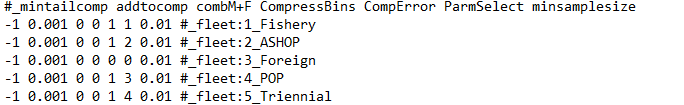
\includegraphics[scale = 0.75]{appendixB_DM_setup}\\
	\end{center}
	
	\item The ParmSelect column can also have repeated values so that multiple fleets share the same log(theta) parameter.
	
	\item If you have both length and age data, the ParmSelect should have separate numbers for each, e.g. 1 and 2 for the length comps and 3 and 4 for the age comps for the same two fleets.
	
\end{itemize}

Add parameter lines to the control file:

\begin{itemize}
	\item Add as many parameter lines as the maximum numbers in the ParmSelect column. The new parameter lines go after the main selectivity parameters but before any time-varying selectivity parameters
	
	\item Jim Thorson initially recommended bounds of -5 to 20, with a starting value of 0
	(which corresponds to a weight of about 50\% of the input sample size). However, parameter estimates above 5 are associated with 99-100\% weight with little information in the likelihood about the parameter value. Therefore, an upper bound of 5 may help identify cases that otherwise would have convergence issues.
	
	\item Example parameter lines are below: 
		\begin{center}
			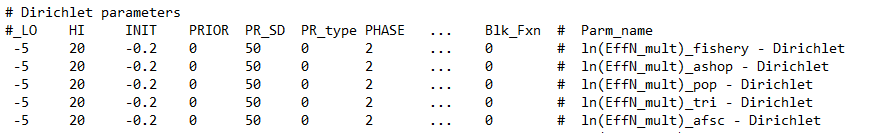
\includegraphics[scale = 0.70]{appendixB_DM_parameters}\\
		\end{center}
	
	\item Reset any existing variance adjustments factors that might have been used for the McAllister-Ianelli or Francis tuning methods. In 3.24 this means setting the values to 1, in SS version 3.30, you can simply delete or comment-out the rows with the adjustments.
\end{itemize}

The \texttt{SS\_output} function in r4ss returns table like the following:

\begin{center}
	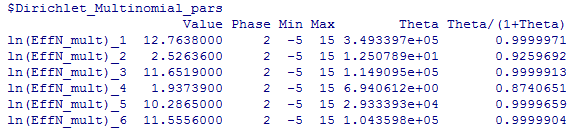
\includegraphics[scale = 1]{appendixB_DM_output}\\
\end{center}

The ratio shown in the final column is the estimated multiplier which can be compared to the sample size adjustment estimated in the other tuning methods above (the New\_Var\_adj column in the table produced by the \texttt{SS\_tune\_comps} function in r4ss).

If the reported $\theta/(1+\theta)$ ratio is close to 1.0, that indicates that the model is trying to tune the sample size as high as possible. In this case, the $ln(\theta)$ parameters should be fixed at a high value, like the upper bound of 20, which will result in 100\% weight being applied to the input sample sizes. An alternative would be to manually change the input sample sizes to a higher value so that the estimated weighting will be less than 100%.

There is also information about this result produced in the plots created by the \texttt{SS\_plots} function:

\begin{center}
	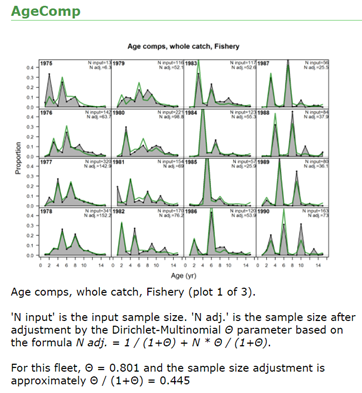
\includegraphics[scale = 1]{appendixB_DM}\\
\end{center}

There are a several of challenges posed by the Dirichlet-Multinomial data-weighting approach:
\begin{enumerate}
	\item Not yet widely used so little guidance is available.
	
	\item Does not allow weights above 100\% (by design) so it is not yet clear how best to deal with the situation when the estimated weight is close to 100\%.
	
	\item Parameterization has potential to cause convergence issues or inefficient MCMC sampling when weights are close to 100\% (Jim Thorson has proposed a prior distribution that may help with this, but has not yet been tested).
\end{enumerate}	
	%========= Section 19: Appendix C: Forecast Module
	%\hypertarget{appendB}{}
\section{Appendix C: Forecast Module}


\subsection{Introduction}
Version 3.20 of Stock Synthesis (SS) introduced substantial upgrades to the benchmark and forecast module.  The general intent was to make the forecast outputs more consistent with the requirement to set catch limits that have a known probability of exceeding the overfishing limit.  In addition, this upgrade addressed several inadequacies with the previous module, including:

\begin{itemize}
	\item The average selectivity and relative F was the same for the benchmark and the forecast calculations;
	\item The biology-at-age in endyr+1 was used as the biology for the benchmark, but biology–at-age propagated forward in the forecast if there was time-varying growth;
	\item The forecast module had a kluge approach to calculation of OFL conditioned on previously catching ABC;
	\item The forecast module implementation of catch caps was incomplete and applied some caps on a seasonally, rather than the more logical annual basis;
	\item The Fmult scalar for fishing intensity presented a confusing concept for many users;
	\item No provision for specification of catch allocation among fleets;
	\item The forecast allowed for a blend of fixed input catches and catches calculated from target F; this is not optimal for calculation of the variance of F conditioned on a catch policy that sets ACLs.
\end{itemize}

The V3.20 module addressed these issues by:
\begin{itemize}
	\item Providing for unique specification of a range of years from which to calculate average selectivity for benchmark, average selectivity for forecast, relative F for benchmark, and relative F for forecast;
	\item Create a new specification for the range of years over which to average size-at-age and fecundity-at-age for the benchmark calculation.  In a setup with time-varying growth, it may make sense to do this over the entire range of years in the time series.  Note that some additional quantities still use their endyr values, notably the migration rates and the allocation of recruitments among areas.  This will be addressed shortly;
	\item Create a multiple pass approach that rectifies the OFL calculation;
	\item Improve the specification of catch caps and implement specification of catch allocations so that there can be an annual cap for each fleet, an annual cap for each area, and an annual allocation among groups of fleets (e.g. all recreational fleets vs. all commercial fleets);
	\item Introduce capability to have implementation error in the forecast catch (single value applied to all fleets in all seasons of the year).
\end{itemize}

\subsection{Multiple Pass Forecast}
The most complicated aspect of the changes is with regard to the multiple pass aspect of the forecast.  This multiple pass approach is needed to calculate both OFL and ABC in a single model run.  More importantly, the multiple passes are needed in order to mimic the actual sequence of assessment-management action – catch over a multi-year period.  The first pass calculates OFL based on catching OFL each year, so presents the absolute maximum upper limit to catches.  The second pass forecasts a catch based on a harvest policy, then applies catch caps and allocations, then updates the F’s to match these catches.  In the third pass, stochastic recruitment and catch implementation error are implemented and SS calculates the F that would be needed in order to catch the adjusted catch amount previously calculated in the second pass.  With this approach, SS is able to produce improved estimates of the probability that F would exceed the overfishing F.  In effect it is the complement of the P* approach.  Rather than the P* approach that calculates the stream of annual catches that would have an annual probability of F>Flimit, SS calculates the expected time series of P* that would result from a specified harvest policy implemented as a buffer between Ftarget and Flimit.

The sequence of multiple forecast passes is as follows:
\begin{enumerate}
	\item Pass 1 (a.k.a. Fcast\_Loop1)
	\begin{enumerate}
		\item Loop Years
		\begin{enumerate}
			\item SubLoop (a.k.a. ABC\_Loop) = 1
			\begin{enumerate}
				\item R=f(SSB) with no deviations
				\item F=Flimit
				\item Fixed input catch amounts ignored
				\item No catch adjustments (caps and allocations)
				\item No implementation error
				\item Result: OFL conditioned on catching OFL each year
			\end{enumerate}
		\end{enumerate}
	\end{enumerate}
	\item Pass 2
	\begin{enumerate}
		\item Loop Years
		\begin{enumerate}
			\item SubLoop = 1
			\begin{enumerate}
				\item R=f(SSB) with no deviations
				\item F=Flimit
				\item Fixed input catch amounts ignored
				\item No catch adjustments (caps and allocations)
				\item No implementation error
				\item Result: OFL conditioned on catching ABC previous year. Stored in std\_vector.
			\end{enumerate}
			\item SubLoop = 2
			\begin{enumerate}
				\item R=f(SSB) with no deviations
				\item F=Ftarget to get catch for each fleet in each season
				\item Fixed input catch amounts replace catch from step 2
				\item Catch adjustments (caps and allocations) applied on annual basis (after looping through seasons and and areas within this year). These adjustments utilize the logistic joiner approach common in SS so the overall results remain completely differentiable.
				\item No implementation error
				\item Result: ABC as adjusted for caps and allocations
			\end{enumerate}
			\item SubLoop = 3
			\begin{enumerate}
				\item R=f(SSB) with no deviations
				\item Catches from Pass 2 multiplied by the random term for implementation error
				\item F=adjusted to match the catch*error while taking into account the random recruitments.  This is most easily visualized in a MCMC context where the recruitment deviation and the implementation error deviations take on non-zero values in each instance.  In MLE, because the forecast recruitments and implementation error are estimated parameters with variance, their variance still propagates to the derived quantities in the forecast.
				\item Result:  Values for F, SSB, Recruitment, Catch are stored in std-vectors
				\begin{itemize}
					\item In addition, the ratios F/Flimit and SSB/SSBlimit or SSB/SSBtarget are also stored in std\_vectors.
					\item Estimated variance in these ratios allows calculation of annual probability that F>Flimit or B<Blimit.  This is essentially the realized P* conditioned on the specified harvest policy.
				\end{itemize}
			\end{enumerate}
		\end{enumerate}
	\end{enumerate}
\end{enumerate}

\subsection{Example Effects on Correlations}
An example that illustrates the above process was conducted.  The situation was a low M, late-maturing species, so changes are not dramatic.  The example conducted a 10 year forecast and examined correlations with derived quantities in the last year of the forecast.  This was done once with the full set of 3 passes as described above, and again with only 2 passes and stochastic recruitment occurring in pass 2, rather than 3.  This alternative setup is more similar to forecasts done using previous model versions.

\begin{center}
	\begin{longtable}{p{0.4cm} p{2.75cm} p{3cm} p{1cm} p{0.4cm} p{2.75cm} p{2cm} p{1cm}}
		\hline
		 & \multicolumn{3}{l}{2 Forecast Passes with F from} & & \multicolumn{3}{l}{2 Forecast Passes with catch from}\\
		 & \multicolumn{3}{l}{ABC and random recruitment} & & \multicolumn{3}{l}{target F and equilibrium recruitment}\\
		\hline
		 & Factor X & Factor Y & Corr &  & Factor X & Factor Y & Corr \\
		 \hline
		 A1 & F 2011 & RecrDev 2002 & -0.126 & A2 & F 2011 & RecrDev 2002 & 0.090 \\
		 B1 & F 2011 & Recr 2002    &  0.312 & B2 & F 2011 & Recr    2002 & 0.518 \\
		 C1 & ForeCatch 2011 & RecrDev 2002 & 0.000 & C2 & ForeCatch 2011 & RecrDev 2002 & 0.129 \\
		 D1 & ForeCatch 2011 & Recr 2002    & 0.455 & D2 & Forecatch 2011 & Recr 2002    & 0.555 \\
		 \hline		
	\end{longtable}
\end{center}

Correlation A2 shows a small positive correlation between the recruitment deviation in 2002 and the F in 2011.  This is probably due to the fact that a positive deviation in recruitment in 2002 will reduce the chances that the biomass in 2011 will be below the inflection point in the control rule.  This occurs because in calculating catch from F, the model effectively “knows” the future recruitments.  I predict that this B1 correlation would be near zero if there was no inflection in the control rule.

Correlation A1 shows this turning into a negative correlation.  This is because the future catches are first calculated from equilibrium recruitment, then when random recruitments are implemented, a positive recruitment deviation will cause a negative deviation in the F needed to catch that now "fixed" amount of future catch.

Correlations B1 and B2 are in terms of absolute recruitment, not recruitment deviation.  Now overall model conditions that cause a higher absolute recruitment level will also result in a higher forecast level.  No surprise there, and the correlation is stronger when variance is based on catch is calculated from F (B2).

Correlation C2 shows a positive correlation between recruitment deviation in 2002 and forecast catch in 2011.  However, correlation C1 is 0.0 because the forecast catch in 2011 is set based on equilibrium recruitment and is not influenced by the recruitment deviations.

\subsection{Future Work}
\begin{itemize}
	\item More testing with high M, rapid turnover conditions
	\item Testing without inflection in control rule
	\item Consider separating implementation error into a pass \#4 so results will more clearly show effect of assessment uncertainty separate from implementation uncertainty
	\item 	Consider adding a random "assessment" error which essentially is a random variable that scales population abundance before passing into the forecast stage.  Complication is figuring out how to link it to the correlated error in the benchmark quantities
	\item Because all of these calculations occur only in the sdphase or the mceval phase, it would be feasible for mceval calls to add an additional pass that is implemented many times and in which random forecast recruitment draws are made.
	\item Factors like selectivity and fleet relative F levels are calculated as an average of these values during the time series.  This is internally consistent if these factors do not vary during the time series (although clearly this is a stiff model that will underestimate process variance).  However, if these factors do vary over time, then the average used for the forecast will under-represent the variance.  A better approach would be to set up the parameters of selectivity as a random process that extends throughout the forecast period, and to update estimated selectivity in each year of the forecast based upon the random realization of these parameters.
\end{itemize}

	
	
	%========= Section 20: Appendix D: Code Examples
	%\section{Appendix D: Code Examples}

\subsection{Ageing Error Estimation}
\hypertarget{AgeingError}{}
%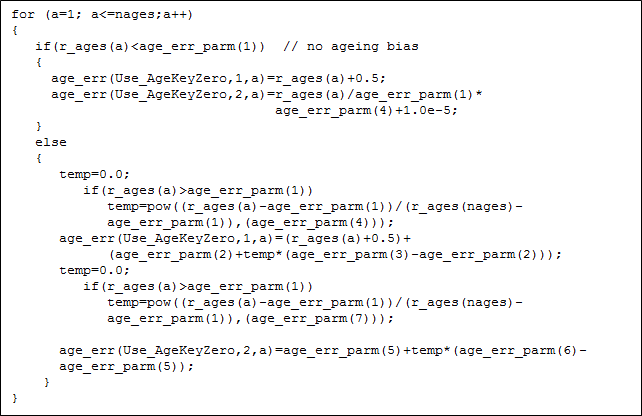
\includegraphics{age_error2}
%The 7 parameters are:

%\begin{itemize}
%	\item age at which the estimated pattern begins (just linear below this age).  This is “start age”
%	\item bias at start age (as additive offset from unbiased age’)
%	\item bias at maxage (as additive offset from unbiased age’)
%	\item power fxn coefficient for interpolating between those 2 values (value of 0.0 produces linear interpolation in the bias)
%	\item stdev at age
%	\item stdev at max age
%	\item power fxn coefficient for interpolating between those 2 values
%\end{itemize}

\scriptsize
\begin{verbatim}
 /*  SS_Label_FUNCTION 45 get_age_age */
 FUNCTION void get_age_age(const int Keynum, const int AgeKey_StartAge, const int AgeKey_Linear1, const int AgeKey_Linear2)
 {
 //  FUTURE: calculate adjustment to oldest age based on continued ageing of old fish
 age_age(Keynum).initialize();
 dvariable age;
 dvar_vector age_err_parm(1,7);
 dvariable temp;
 
 if(Keynum==Use_AgeKeyZero)
 {
 //  SS_Label_45.1 set age_err_parm to mgp_adj, so can be time-varying according to MGparm options
 for (a=1;a<=7;a++)
 {age_err_parm(a)=mgp_adj(AgeKeyParm-1+a);}
 age_err(Use_AgeKeyZero,1)(0,AgeKey_StartAge)=r_ages(0,AgeKey_StartAge)+0.5;
 age_err(Use_AgeKeyZero,2)(0,AgeKey_StartAge)=age_err_parm(5)*(r_ages(0,AgeKey_StartAge)+0.5)/
 (age_err_parm(1)+0.5);
 //  SS_Label_45.3 calc ageing bias
 if(AgeKey_Linear1==0)
 {
 age_err(Use_AgeKeyZero,1)(AgeKey_StartAge,nages)=0.5 + r_ages(AgeKey_StartAge,nages) + 
 age_err_parm(2)+(age_err_parm(3)-age_err_parm(2))*(1.0-mfexp(-age_err_parm(4)*
 (r_ages(AgeKey_StartAge,nages)-age_err_parm(1)))) / (1.0-mfexp(-age_err_parm(4)*
 (r_ages(nages)-age_err_parm(1))));
 }
 else
 {
 age_err(Use_AgeKeyZero,1)(AgeKey_StartAge,nages)=0.5 + r_ages(AgeKey_StartAge,nages) + 
 age_err_parm(2)+(age_err_parm(3)-age_err_parm(2))*
 (r_ages(AgeKey_StartAge,nages)-age_err_parm(1))/(r_ages(nages)-age_err_parm(1));
 }
 //  SS_Label_45.4 calc ageing variance
 if(AgeKey_Linear2==0)
 {
 age_err(Use_AgeKeyZero,2)(AgeKey_StartAge,nages)=age_err_parm(5)+(age_err_parm(6)-age_err_parm(5))*
 (1.0-mfexp(-age_err_parm(7)*(r_ages(AgeKey_StartAge,nages)-age_err_parm(1)))) / 
 (1.0-mfexp(-age_err_parm(7)*(r_ages(nages)-age_err_parm(1))));
 }
 else
 {
 age_err(Use_AgeKeyZero,2)(AgeKey_StartAge,nages)=age_err_parm(5)+(age_err_parm(6)-age_err_parm(5))*
 (r_ages(AgeKey_StartAge,nages)-age_err_parm(1))/(r_ages(nages)-age_err_parm(1));
 }
 }
\end{verbatim}


\subsection{Survival Based SRR Code}
\hypertarget{AppendixC}{Code} for the survival based recruitment is shown below:\\
%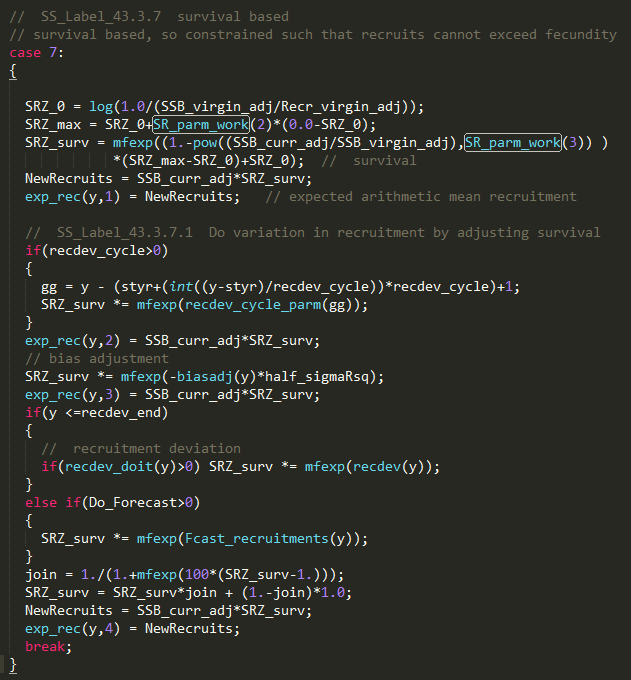
\includegraphics{survival_code_330}

\scriptsize
\begin{verbatim}
//  SS_Label_43.3.7  survival based
case 7:  // survival based, so constrained such that recruits cannot exceed fecundity
{

SRZ_0=log(1.0/(SSB_virgin_adj/Recr_virgin_adj));
SRZ_max=SRZ_0+SR_parm_work(2)*(0.0-SRZ_0);
SRZ_surv=mfexp((1.-pow((SSB_curr_adj/SSB_virgin_adj),SR_parm_work(3)) )*(SRZ_max-SRZ_0)+SRZ_0);  //  survival
NewRecruits=SSB_curr_adj*SRZ_surv;
exp_rec(y,1)=NewRecruits;   // expected arithmetic mean recruitment

//  SS_Label_43.3.7.1  Do variation in recruitment by adjusting survival
if(recdev_cycle>0)
{
gg=y - (styr+(int((y-styr)/recdev_cycle))*recdev_cycle)+1;
SRZ_surv*=mfexp(recdev_cycle_parm(gg));
}
exp_rec(y,2)=SSB_curr_adj*SRZ_surv;
SRZ_surv*=mfexp(-biasadj(y)*half_sigmaRsq);     // bias adjustment
exp_rec(y,3)=SSB_curr_adj*SRZ_surv;
if(y <=recdev_end)
{
if(recdev_doit(y)>0) SRZ_surv*=mfexp(recdev(y));  //  recruitment deviation
}
else if(Do_Forecast>0)
{
SRZ_surv *= mfexp(Fcast_recruitments(y));
}
join=1./(1.+mfexp(100*(SRZ_surv-1.)));
SRZ_surv=SRZ_surv*join + (1.-join)*1.0;
NewRecruits=SSB_curr_adj*SRZ_surv;
exp_rec(y,4) = NewRecruits;
break;
}
\end{verbatim}

\pagebreak
\subsection{Random Walk Selectivity: Pattern 17}
\hypertarget{RandWalkSelex}{Code} for selectivity pattern 17, random walk shown below:
%	\begin{center}
%		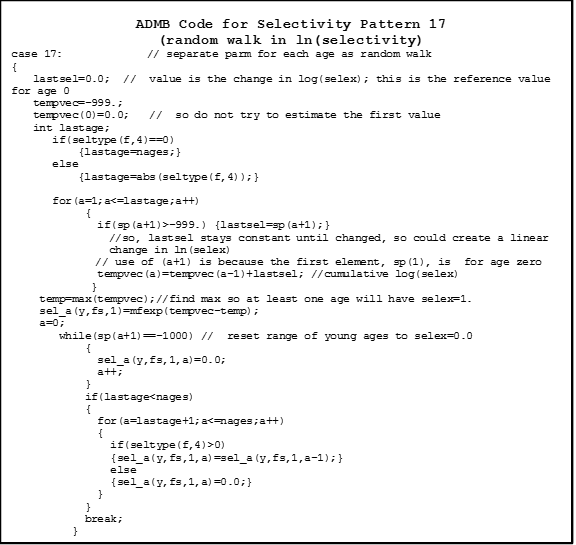
\includegraphics{Selex17_RandomWalk}
%	\end{center}	
\scriptsize{
	\begin{verbatim}
	 
	 //  SS_Label_Info_22.7.17 #age selectivity: each age has parameter as random walk
	 // #41 each age has parameter as random walk scaled by average of values at low age through high age
	 //    transformation as selex=exp(parm); some special codes */
	 case 41:
	 scaling_offset = 2;
	 case 17:                  //
	 {
	 lastsel=0.0;  //  value is the change in log(selex);  this is the reference value for age 0
	 tempvec_a=-999.;
	 tempvec_a(0)=0.0;   //  so do not try to estimate the first value
	 int lastage;
	 if(seltype(f,4)==0)
	 {lastage=nages;}
	 else
	 {lastage=abs(seltype(f,4));}
	 
	 for (a=1;a<=lastage;a++)
	 {
	 //  with use of -999, lastsel stays constant until changed, so could create a linear change in ln(selex)
	 // use of (a+1) is because the first element, sp(1), is for age zero
	 if(sp(a+1+scaling_offset)>-999.) {lastsel=sp(a+1+scaling_offset);}
	 tempvec_a(a)=tempvec_a(a-1)+lastsel;   // cumulative log(selex)
	 }
	 if (scaling_offset == 0)
	 {
	 temp=max(tempvec_a);   //  find max so at least one age will have selex=1.
	 }
	 else
	 {
	 int low_bin  = int(value(sp(1)));
	 int high_bin = int(value(sp(2)));
	 if (low_bin < 0)
	 {
	 low_bin = 0;
	 N_warn++; warning<<" selex pattern 41; value for low bin is less than 0, so set to 0 "<<endl;
	 }
	 if (high_bin > nages)
	 {
	 high_bin = nages;
	 N_warn++; warning<<" selex pattern 41; value for high bin is greater than "<<nages<<", so set to "<<nages<<" "<<endl;
	 }
	 if (high_bin < low_bin) high_bin = low_bin;
	 if (low_bin > high_bin) low_bin = high_bin;
	 sp(1) = low_bin;
	 sp(2) = high_bin;
	 temp=mean(tempvec_a(low_bin,high_bin));
	 }
	 sel_a(y,fs,1)=mfexp(tempvec_a-temp);
	 a=0;
	 while(sp(a+1+scaling_offset)==-1000)  //  reset range of young ages to selex=0.0
	 {
	 sel_a(y,fs,1,a)=0.0;
	 a++;
	 }
	 scaling_offset = 0;     // reset scaling offset
	 if(lastage<nages)
	 {
	 for (a=lastage+1;a<=nages;a++)
	 {
	 if(seltype(f,4)>0)
	 {sel_a(y,fs,1,a)=sel_a(y,fs,1,a-1);}
	 else
	 {sel_a(y,fs,1,a)=0.0;}
	 }
	 }
	 break;
	 }  
	\end{verbatim}

\pagebreak
\subsection{Cubic Spline Selectivity}
\hypertarget{CubicSpline}{Code} for cubic spline selectivity, option 42, shown below:
%	\begin{center}
%		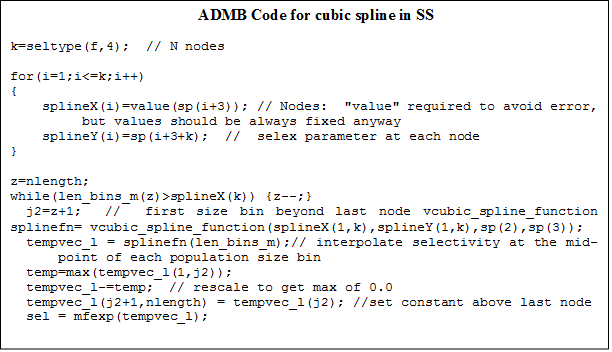
\includegraphics{CubicSplineCode}
%	\end{center}

\scriptsize
\begin{verbatim}
	
	//  SS_Label_Info_22.7.27 #age selectivity: cubic spline
	// #42 cubic spline scaled by average of values at low age through high age
	case 42:
	scaling_offset = 2;
	case 27:
	{
	k=seltype(f,4);  // n points to include in cubic spline
	for (i=1;i<=k;i++)
	{
	splineX(i)=value(sp(i+3+scaling_offset)); // "value" required to avoid error, but values should be always fixed anyway
	splineY(i)=sp(i+3+k+scaling_offset);
	}
	z=nages;
	while(r_ages(z)>splineX(k)) {z--;}
	j2=z+1;  //  first age beyond last node
	vcubic_spline_function splinefn=vcubic_spline_function(splineX(1,k),splineY(1,k),sp(2+scaling_offset),sp(3+scaling_offset));
	tempvec_a= splinefn(r_ages);  // interpolate selectivity at each age
	if (scaling_offset == 0)
	{
	temp=max(tempvec_a(0,j2));
	}
	else
	{
	int low_bin  = int(value(sp(1)));
	int high_bin = int(value(sp(2)));
	if (low_bin < 0)
	{
	low_bin = 0;
	N_warn++; warning<<" selex pattern 42; value for low bin is less than 0, so set to 0 "<<endl;
	}
	if (high_bin > nages)
	{
	high_bin = nages;
	N_warn++; warning<<" selex pattern 42; value for high bin is greater than "<<nages<<", so set to "<<nages<<" "<<endl;
	}
	if (high_bin < low_bin) high_bin = low_bin;
	if (low_bin > high_bin) low_bin = high_bin;
	sp(1) = low_bin;
	sp(2) = high_bin;
	temp=mean(tempvec_a(low_bin,high_bin));
	scaling_offset = 0;     // reset scaling offset
	}
	tempvec_a-=temp;  // rescale to get max of 0.0
	tempvec_a(j2+1,nages) = tempvec_a(j2);  //  set constant above last node
	sel_a(y,fs,1)=mfexp(tempvec_a);
	break;
	}
	
\end{verbatim}

\pagebreak
\subsection{Deviation Link}
\hypertarget{DevLink}{Code} for alternative deviation links shown below:

\scriptsize
\begin{verbatim}

    case 1 (multiplicative):
    {
      for (j=timevary_setup(10);j<=timevary_setup(11);j++)
      {
        parm_timevary(tvary,j)*=mfexp(parm_dev(k,j)*parm_dev_stddev(k));
      }
      break;
    }

    case 2 (additive):
    {
      for (j=timevary_setup(10);j<=timevary_setup(11);j++)
      {
        parm_timevary(tvary,j)+=parm_dev(k,j)*parm_dev_stddev(k);
      }
      break;
    }

    case 3 (random walk):
    {
      parm_dev_rwalk(k,timevary_setup(10))=parm_dev(k,timevary_setup(10))*parm_dev_stddev(k);
      parm_timevary(tvary,timevary_setup(10))+=parm_dev_rwalk(k,timevary_setup(10));
      for (j=timevary_setup(10)+1;j<=timevary_setup(11);j++)
      {
        parm_dev_rwalk(k,j)=parm_dev_rwalk(k,j-1)+parm_dev(k,j)*parm_dev_stddev(k);
        parm_timevary(tvary,j)+=parm_dev_rwalk(k,j);
      }
      break;
    }

    case 4 (mean reverting random walk)
    {
      parm_dev_rwalk(k,timevary_setup(10))=parm_dev(k,timevary_setup(10))*parm_dev_stddev(k);
      parm_timevary(tvary,timevary_setup(10))+=parm_dev_rwalk(k,timevary_setup(10));
      for (j=timevary_setup(10)+1;j<=timevary_setup(11);j++)
      {
        //    =(1-rho)*mean + rho*prevval + dev   //  where mean = 0.0
        parm_dev_rwalk(k,j)=parm_dev_rho(k)*parm_dev_rwalk(k,j-1)+parm_dev(k,j)*parm_dev_stddev(k);
        parm_timevary(tvary,j)+=parm_dev_rwalk(k,j);
      }
      break;
    }
	
\end{verbatim}

\pagebreak	
	%========= Section 21: Appendix E: In process and wish list
	%\section{Appendix E: In Process and Wish List Items for Future Versions}

\begin{center}
	\begin{longtable}{p{2cm} p{3cm} p{10cm}}
		Category & Item & Description\\
		\hline
		\endfirsthead
				
		Category & Item & Description\\
		\hline
		\endhead
				
		\hline
		\endfoot
				
		\endlastfoot
		
		In process 
		  &	Environmental survey of a deviation vector & Environmental survey data can be related to f(a deviation vector), but needs more Q\_link functions.\\
		  \\
		  & Retrospective & Make blocks work when doing retrospective analyses. \\
		
		\hline
		Wishlist & &
			 Tag-recapture major revamp\\\\
	     & & Area specific spawner-recruitment \\\\
	     & & Add automatic set-up for size selectivity option 6 and age selectivity option 17 given the data (comparable to the current capacity for cubic spline selectivity).\\\\
	     & & More error checking on read of empirical weight-at-age and composition data. \\\\
	     & & New version of age-specific K needed because current version is inefficient.\\\\
	     & & Mean size in plus group uses a fixed erosion factor of 0.2; should be context specific. \\\\
	     & & Consider Tim Miller's state space model approach. \\\\
	     & & Add other options to CV growth patter for log(SD). \\\\
	     & & Add measure of auto-correlation in composition and in survey residuals.\\\\
	     & & Add SD report for survey expected values. \\\\
	     & & Add calculation of Francis composition weighting method. \\\\
	     & & Year-specific MSY.	     	   \\	  	  				
		\hline
	\end{longtable}
\end{center}


	%========= Section 22: Appendix F: Input files
	%\begin{landscape}

\section{Appendix F: Example Model Files}


\subsection{starter.ss}
\scriptsize{
\begin{verbatim}
  #V3.30.10.00-safe;_2018_01_09;_Stock_Synthesis_by_Richard_Methot_(NOAA)_using_ADMB_11.6
  #_user_support_available_at:NMFS.Stock.Synthesis@noaa.gov
  #_user_info_available_at:https://vlab.ncep.noaa.gov/group/stock-synthesis
  #C starter comment here
  simple.dat
  simple.ctl
  0 # 0=use init values in control file; 1=use ss.par
  1 # run display detail (0,1,2)
  1 # detailed age-structured reports in REPORT.SSO (0=low,1=high,2=low for data-limited) 
  0 # write detailed checkup.sso file (0,1) 
  4 # write parm values to ParmTrace.sso (0=no,1=good,active; 2=good,all; 3=every_iter,all_parms; 4=every,active)
  1 # write to cumreport.sso (0=no,1=like&timeseries; 2=add survey fits)
  1 # Include prior_like for non-estimated parameters (0,1) 
  1 # Use Soft Boundaries to aid convergence (0,1) (recommended)
  3 # Number of datafiles to produce: 1st is input, 2nd is estimates, 3rd and higher are bootstrap
  10 # Turn off estimation for parameters entering after this phase
  0 # MCeval burn interval
  1 # MCeval thin interval
  0 # jitter initial parm value by this fraction
  1969 # min yr for sdreport outputs (-1 for styr)
  2011 # max yr for sdreport outputs (-1 for endyr; -2 for endyr+Nforecastyrs
  0 # N individual STD years 
  #vector of year values 
  0.0001 # final convergence criteria (e.g. 1.0e-04) 
  0 # retrospective year relative to end year (e.g. -4)
  1 # min age for calc of summary biomass
  1 # Depletion basis:  denom is: 0=skip; 1=rel X*B0; 2=rel X*Bmsy; 3=rel X*B_styr
  0.4 # Fraction (X) for Depletion denominator (e.g. 0.4)
  1 # SPR_report_basis:  0=skip; 1=(1-SPR)/(1-SPR_tgt); 2=(1-SPR)/(1-SPR_MSY); 3=(1-SPR)/(1-SPR_Btarget); 4=rawSPR
  4 # F_report_units: 0=skip; 1=exploitation(Bio); 2=exploitation(Num); 3=sum(Frates); 4=true F for range of ages
  20 23 #_min and max age over which average F will be calculated
  1 # F_report_basis: 0=raw_F_report; 1=F/Fspr; 2=F/Fmsy ; 3=F/Fbtgt
  0 # MCMC output detail (0=default; 1=obj func components; 2=expanded; 3=make output subdir for each MCMC vector)
  0 # ALK tolerance (example 0.0001)
  3.30 # check value for end of file and for version control
\end{verbatim}
}


\subsection{forecast.ss}
\scriptsize{
\begin{verbatim}
  #V3.30.10.00-safe;_2018_01_09;_Stock_Synthesis_by_Richard_Methot_(NOAA)_using_ADMB_11.6
  #C  generic forecast file
  # for all year entries except rebuilder; enter either: actual year, -999 for styr, 0 for endyr, neg number for rel. endyr
  1 # Benchmarks: 0=skip; 1=calc F_spr,F_btgt,F_msy; 2=calc F_spr,F0.1,F_msy 
  2 # MSY: 1= set to F(SPR); 2=calc F(MSY); 3=set to F(Btgt) or F0.1; 4=set to F(endyr) 
  0.4 # SPR target (e.g. 0.40)
  0.342 # Biomass target (e.g. 0.40)
  #_Bmark_years: beg_bio, end_bio, beg_selex, end_selex, beg_relF, end_relF, beg_recr_dist, end_recr_dist, beg_SRparm, end_SRparm (enter actual year, or values of 0 or -integer to be rel. endyr)
  2001 2001 2001 2001 2001 2001 1971 2001 1971 2001
  1 #Bmark_relF_Basis: 1 = use year range; 2 = set relF same as forecast below
  #
  1 # Forecast: 0=none; 1=F(SPR); 2=F(MSY) 3=F(Btgt) or F0.1; 4=Ave F (uses first-last relF yrs); 5=input annual F scalar
  10 # N forecast years 
  0.2 # F scalar (only used for Do_Forecast==5)
  #_Fcast_years:  beg_selex, end_selex, beg_relF, end_relF, beg_recruits, end_recruits  (enter actual year, or values of 0 or -integer to be rel. endyr)
  0 0 -10 0 -999 0
  0 # Forecast selectivity (0=fcast selex is mean from year range; 1=fcast selectivity from annual time-vary parms)
  1 # Control rule method (1=catch=f(SSB) west coast; 2=F=f(SSB) ) 
  0.4 # Control rule Biomass level for constant F (as frac of Bzero, e.g. 0.40); (Must be > the no F level below) 
  0.1 # Control rule Biomass level for no F (as frac of Bzero, e.g. 0.10) 
  0.75 # Control rule target as fraction of Flimit (e.g. 0.75) 
  3 #_N forecast loops (1=OFL only; 2=ABC; 3=get F from forecast ABC catch with allocations applied)
  3 #_First forecast loop with stochastic recruitment
  0 #_Forecast recruitment:  0= spawn_recr; 1=value*spawn_recr_fxn; 2=value*VirginRecr; 3=recent mean) 
  1 # value is ignored 
  0 #_Forecast loop control #5 (reserved for future bells&whistles) 
  2010  #FirstYear for caps and allocations (should be after years with fixed inputs) 
  0 # stddev of log(realized catch/target catch) in forecast (set value>0.0 to cause active impl_error)
  0 # Do West Coast gfish rebuilder output (0/1) 
  1999 # Rebuilder:  first year catch could have been set to zero (Ydecl)(-1 to set to 1999)
  2002 # Rebuilder:  year for current age structure (Yinit) (-1 to set to endyear+1)
  1 # fleet relative F:  1=use first-last alloc year; 2=read seas, fleet, alloc list below
  # Note that fleet allocation is used directly as average F if Do_Forecast=4 
  2 # basis for fcast catch tuning and for fcast catch caps and allocation  (2=deadbio; 3=retainbio; 5=deadnum; 6=retainnum)
  # Conditional input if relative F choice = 2
  # enter list of:  season,  fleet, relF; if used, terminate with season=-9999
  # 1 1 1
  # enter list of: fleet number, max annual catch for fleets with a max; terminate with fleet=-9999
  -9999 -1
  # enter list of area ID and max annual catch; terminate with area=-9999
  -9999 -1
  # enter list of fleet number and allocation group assignment, if any; terminate with fleet=-9999
  -9999 -1
  #_if N allocation groups >0, list year, allocation fraction for each group 
  # list sequentially because read values fill to end of N forecast
  # terminate with -9999 in year field 
  # no allocation groups
  2 # basis for input Fcast catch: -1=read basis with each obs; 2=dead catch; 3=retained catch; 99=input Hrate(F)
  #enter list of Fcast catches; terminate with line having year=-9999
  #_Yr Seas Fleet Catch(or_F)
  -9999 1 1 0 
  #
  999 # verify end of input  
\end{verbatim}
}



\subsection{data.ss}
\scriptsize{
\begin{verbatim}
  #V3.30.10.00-safe;_2018_01_09;_Stock_Synthesis_by_Richard_Methot_(NOAA)_using_ADMB_11.6
  #_user_support_available_at:NMFS.Stock.Synthesis@noaa.gov
  #_user_info_available_at:https://vlab.ncep.noaa.gov/group/stock-synthesis
  #_Start_time: Fri Feb  2 10:54:21 2018
  #_Number_of_datafiles: 3
  #C data file for simple example
  #_observed data: 
  #V3.30.10.00-safe;_2018_01_09;_Stock_Synthesis_by_Richard_Methot_(NOAA)_using_ADMB_11.6
  1971 #_StartYr
  2001 #_EndYr
  1 #_Nseas
  12 #_months/season
  2 #_Nsubseasons (even number, minimum is 2)
  1 #_spawn_month
  2 #_Ngenders
  40 #_Nages=accumulator age
  1 #_Nareas
  3 #_Nfleets (including surveys)
  #_fleet_type: 1=catch fleet; 2=bycatch only fleet; 3=survey; 4=ignore 
  #_survey_timing: -1=for use of catch-at-age to override the month value associated with a datum 
  #_fleet_area:  area the fleet/survey operates in 
  #_units of catch:  1=bio; 2=num (ignored for surveys; their units read later)
  #_catch_mult: 0=no; 1=yes
  #_rows are fleets
  #_fleet_type timing area units need_catch_mult fleetname
  1 0.5 1 1 0 FISHERY1  # 1
  3 0.5 1 2 0 SURVEY1  # 2
  3 0.5 1 2 0 SURVEY2  # 3
  #Bycatch_fleet_input_goes_next
  #a:  fleet index
  #b:  1=include dead bycatch in total dead catch for F0.1 and MSY optimizations and forecast ABC; 2=omit from total catch for these purposes (but still include the mortality)
  #c:  1=Fmult scales with other fleets; 2=bycatch F constant at input value; 3=bycatch F from range of years
  #d:  F or first year of range
  #e:  last year of range
  #f:  not used
  # a   b   c   d   e   f 
  #_Catch data: yr, seas, fleet, catch, catch_se
  #_catch_se:  standard error of log(catch)
  #_NOTE:  catch data is ignored for survey fleets
  -999 1 1 0 0.01
  1971 1 1 0 0.01
  1972 1 1 200 0.01
  1973 1 1 1000 0.01
  1974 1 1 1000 0.01
  1975 1 1 2000 0.01
  1976 1 1 3000 0.01
  1977 1 1 4000 0.01
  1978 1 1 5000 0.01
  1979 1 1 6000 0.01
  1980 1 1 8000 0.01
  1981 1 1 10000 0.01
  1982 1 1 10000 0.01
  1983 1 1 10000 0.01
  1984 1 1 10000 0.01
  1985 1 1 10000 0.01
  1986 1 1 10000 0.01
  1987 1 1 10000 0.01
  1988 1 1 9000 0.01
  1989 1 1 8000 0.01
  1990 1 1 7000 0.01
  1991 1 1 6000 0.01
  1992 1 1 4000 0.01
  1993 1 1 4000 0.01
  1994 1 1 4000 0.01
  1995 1 1 4000 0.01
  1996 1 1 4000 0.01
  1997 1 1 3000 0.01
  1998 1 1 3000 0.01
  1999 1 1 3000 0.01
  2000 1 1 3000 0.01
  2001 1 1 3000 0.01
  -9999 0 0 0 0
  #
  #_CPUE_and_surveyabundance_observations
  #_Units:  0=numbers; 1=biomass; 2=F; >=30 for special types
  #_Errtype:  -1=normal; 0=lognormal; >0=T
  #_SD_Report: 0=no sdreport; 1=enable sdreport
  #_Fleet Units Errtype SD_Report
  1 1 0 0 # FISHERY1
  2 1 0 0 # SURVEY1
  3 0 0 0 # SURVEY2
  #_yr month fleet obs stderr
  1977 7 2 339689 0.3 #_ SURVEY1
  1980 7 2 193353 0.3 #_ SURVEY1
  1983 7 2 151984 0.3 #_ SURVEY1
  1986 7 2 55221.8 0.3 #_ SURVEY1
  1989 7 2 59232.3 0.3 #_ SURVEY1
  1992 7 2 31137.5 0.3 #_ SURVEY1
  1995 7 2 35845.4 0.3 #_ SURVEY1
  1998 7 2 27492.6 0.3 #_ SURVEY1
  2001 7 2 37338.3 0.3 #_ SURVEY1
  1990 7 3 5.19333 0.7 #_ SURVEY2
  1991 7 3 1.1784 0.7 #_ SURVEY2
  1992 7 3 5.94383 0.7 #_ SURVEY2
  1993 7 3 0.770106 0.7 #_ SURVEY2
  1994 7 3 16.318 0.7 #_ SURVEY2
  1995 7 3 1.36339 0.7 #_ SURVEY2
  1996 7 3 4.76482 0.7 #_ SURVEY2
  1997 7 3 51.0707 0.7 #_ SURVEY2
  1998 7 3 1.36095 0.7 #_ SURVEY2
  1999 7 3 0.862531 0.7 #_ SURVEY2
  2000 7 3 5.97125 0.7 #_ SURVEY2
  2001 7 3 1.69379 0.7 #_ SURVEY2
  -9999 1 1 1 1 # terminator for survey observations 
  #
  0 #_N_fleets_with_discard
  #_discard_units (1=same_as_catchunits(bio/num); 2=fraction; 3=numbers)
  #_discard_errtype:  >0 for DF of T-dist(read CV below); 0 for normal with CV; -1 for normal with se; -2 for lognormal; -3 for trunc normal with CV
  # note, only have units and errtype for fleets with discard 
  #_Fleet units errtype
  # -9999 0 0 0.0 0.0 # terminator for discard data 
  #
  0 #_use meanbodysize_data (0/1)
  #_COND_0 #_DF_for_meanbodysize_T-distribution_like
  # note:  use positive partition value for mean body wt, negative partition for mean body length 
  #_yr month fleet part obs stderr
  #  -9999 0 0 0 0 0 # terminator for mean body size data 
  #
  # set up population length bin structure (note - irrelevant if not using size data and using empirical wtatage
  2 # length bin method: 1=use databins; 2=generate from binwidth,min,max below; 3=read vector
  2 # binwidth for population size comp 
  10 # minimum size in the population (lower edge of first bin and size at age 0.00) 
  94 # maximum size in the population (lower edge of last bin) 
  1 # use length composition data (0/1)
  #_mintailcomp: upper and lower distribution for females and males separately are accumulated until exceeding this level.
  #_addtocomp:  after accumulation of tails; this value added to all bins
  #_males and females treated as combined gender below this bin number 
  #_compressbins: accumulate upper tail by this number of bins; acts simultaneous with mintailcomp; set=0 for no forced accumulation
  #_Comp_Error:  0=multinomial, 1=dirichlet
  #_Comp_Error2:  parm number  for dirichlet
  #_minsamplesize: minimum sample size; set to 1 to match 3.24, minimum value is 0.001
  #_mintailcomp addtocomp combM+F CompressBins CompError ParmSelect minsamplesize
  0 1e-07 0 0 0 0 0.001 #_fleet:1_FISHERY1
  0 1e-07 0 0 0 0 0.001 #_fleet:2_SURVEY1
  0 1e-07 0 0 0 0 0.001 #_fleet:3_SURVEY2
  # sex codes:  0=combined; 1=use female only; 2=use male only; 3=use both as joint sexxlength distribution
  # partition codes:  (0=combined; 1=discard; 2=retained
  25 #_N_LengthBins; then enter lower edge of each length bin
  26 28 30 32 34 36 38 40 42 44 46 48 50 52 54 56 58 60 62 64 68 72 76 80 90
  #_yr month fleet sex part Nsamp datavector(female-male)
  1971 7 1 3 0 125 0 0 0 0 0 0 0 0 0 4 1 1 2 4 1 5 6 2 3 11 8 4 5 0 0 0 0 0 0 0 0 0 0 1 0 1 3 0 3 4 2 4 5 9 17 8 3 8 0 0
  1972 7 1 3 0 125 0 0 0 0 0 0 0 0 0 3 0 1 2 1 1 6 2 7 4 10 10 4 5 3 0 0 0 0 0 0 0 0 0 1 3 2 4 1 3 1 4 4 7 3 8 11 4 10 0 0
  1973 7 1 3 0 125 0 0 0 0 0 0 0 0 0 0 0 0 7 3 4 5 6 3 10 12 6 10 9 0 0 0 0 0 0 0 0 0 0 0 0 0 3 0 1 3 0 7 2 6 7 8 5 5 3 0
  1974 7 1 3 0 125 0 0 0 0 0 0 0 0 0 2 2 0 1 1 1 4 5 3 8 8 10 4 7 0 0 0 0 0 0 0 0 0 1 2 0 4 0 0 1 5 6 6 4 6 15 11 5 0 3 0
  1975 7 1 3 0 125 0 0 0 0 0 0 0 2 1 2 1 1 3 0 2 5 6 2 3 5 9 10 10 0 0 0 0 0 0 0 0 0 0 0 4 2 2 1 2 3 5 1 4 5 13 11 6 4 0 0
  1976 7 1 3 0 125 0 0 0 0 0 0 0 2 1 0 2 2 0 3 2 3 3 3 7 18 14 4 2 2 0 0 0 0 0 0 0 1 0 0 0 0 0 1 2 4 6 6 5 7 12 6 4 3 0 0
  1977 7 1 3 0 125 0 0 0 0 0 0 0 1 0 2 0 2 2 4 0 2 6 7 5 11 7 8 5 4 0 0 0 0 0 0 2 1 3 0 1 3 3 2 0 1 4 5 3 7 7 9 5 3 0 0
  1978 7 1 3 0 125 0 0 0 0 0 0 5 1 1 1 0 1 3 1 8 4 4 6 5 9 8 3 6 5 0 0 0 0 0 0 0 0 2 1 1 2 1 1 2 2 4 1 4 1 13 9 6 4 0 0
  1979 7 1 3 0 125 0 0 0 0 0 0 0 0 0 0 3 5 2 1 5 0 5 5 2 7 4 7 5 5 0 0 0 0 0 0 0 0 0 2 2 1 3 2 7 2 4 4 5 8 10 8 6 4 1 0
  1980 7 1 3 0 125 0 0 0 0 0 0 0 4 0 0 1 0 2 4 3 2 3 2 3 16 11 12 4 2 0 0 0 0 0 0 0 0 0 1 4 1 1 2 3 5 2 6 3 1 10 11 4 2 0 0
  1981 7 1 3 0 125 0 0 0 0 0 0 1 0 0 0 3 1 2 2 4 5 2 7 3 13 9 8 4 0 0 0 0 0 0 0 2 1 1 1 2 2 3 3 1 6 1 2 1 7 5 10 6 7 0 0
  1982 7 1 3 0 125 0 0 0 0 0 0 0 0 5 2 1 3 2 3 8 2 5 4 4 6 10 11 0 0 0 0 0 0 0 0 0 0 1 0 3 0 2 1 5 6 1 8 5 5 10 5 2 5 0 0
  1983 7 1 3 0 125 0 0 0 0 0 0 0 0 0 0 7 1 1 5 4 2 2 6 2 8 13 8 6 0 0 0 0 0 0 0 0 0 0 0 4 1 0 3 3 0 4 9 5 4 7 8 6 6 0 0
  1984 7 1 3 0 125 0 0 0 0 0 0 1 0 0 4 3 0 3 1 2 5 2 4 7 11 9 6 8 0 0 0 0 0 0 0 0 0 3 3 1 1 3 3 3 2 2 4 4 8 11 4 5 2 0 0
  1985 7 1 3 0 125 0 0 0 0 0 0 0 0 1 1 2 2 5 0 3 3 5 11 4 8 9 3 2 4 0 0 0 0 0 0 0 0 1 0 1 2 0 3 8 3 4 3 8 4 13 7 4 1 0 0
  1986 7 1 3 0 125 0 0 0 3 1 0 1 2 0 4 2 0 0 4 2 8 3 5 11 5 6 6 1 0 0 0 0 0 0 0 2 2 0 1 2 1 3 4 2 3 4 6 5 5 6 4 6 5 0 0
  1987 7 1 3 0 125 0 0 0 0 1 1 1 1 1 0 2 1 6 4 2 7 6 3 5 11 9 5 4 0 0 0 0 0 0 0 0 0 2 1 0 5 2 4 3 4 4 4 2 4 7 6 5 2 0 0
  1988 7 1 3 0 125 0 0 0 0 0 2 0 1 4 2 1 1 2 2 1 7 4 5 6 9 9 2 1 0 0 0 0 0 0 0 2 1 1 3 1 3 6 3 3 0 4 5 3 5 9 9 8 0 0 0
  1989 7 1 3 0 125 0 0 0 0 0 1 0 2 1 3 3 2 1 4 4 3 4 2 3 9 5 11 2 0 0 0 0 0 0 0 0 3 6 2 1 3 0 4 3 3 2 5 7 7 9 3 3 4 0 0
  1990 7 1 3 0 125 0 0 0 0 0 0 0 2 2 2 2 2 2 2 9 4 4 6 6 8 4 4 1 0 0 0 0 0 0 0 1 1 2 2 3 8 2 8 6 6 3 2 3 4 6 5 1 2 0 0
  1991 7 1 3 0 125 0 0 0 0 0 0 0 3 0 3 3 5 5 4 3 3 0 1 6 10 4 4 0 0 0 0 0 0 0 1 1 1 1 3 4 6 5 3 5 6 6 6 6 4 7 3 3 0 0 0
  1992 7 1 3 0 125 0 0 0 0 2 2 0 1 1 1 3 3 2 7 6 4 4 2 5 6 3 6 0 0 0 0 0 0 0 0 0 0 5 3 1 3 5 3 5 8 3 4 6 3 13 4 1 0 0 0
  1993 7 1 3 0 125 0 0 0 0 0 0 1 2 2 2 2 2 4 5 10 5 7 3 2 12 7 6 0 0 0 0 0 0 0 0 0 0 3 1 1 3 2 6 4 8 4 6 4 2 4 3 1 1 0 0
  1994 7 1 3 0 125 0 0 0 0 0 0 0 0 0 4 1 4 3 4 4 9 4 6 7 8 5 3 2 0 0 0 0 0 0 0 0 0 2 0 2 1 1 4 4 10 5 8 6 3 5 6 1 3 0 0
  1995 7 1 3 0 125 0 0 0 1 0 0 1 1 1 1 2 2 5 8 4 11 5 5 4 8 7 0 0 0 0 0 0 0 0 1 0 0 1 1 3 3 1 2 6 3 4 4 8 3 12 4 3 0 0 0
  1996 7 1 3 0 125 0 0 0 1 0 2 1 0 2 4 3 3 2 3 6 6 3 3 4 11 6 6 0 0 0 0 0 0 0 0 0 1 2 0 3 3 1 0 5 4 6 7 4 5 10 3 4 1 0 0
  1997 7 1 3 0 125 0 0 0 2 0 0 2 2 0 0 3 1 6 4 6 2 9 4 5 9 12 0 0 0 0 0 0 0 0 0 3 1 0 5 3 2 4 1 1 6 4 1 6 6 5 6 4 0 0 0
  1998 7 1 3 0 125 0 0 0 0 3 1 2 2 2 2 3 1 3 6 2 0 7 4 5 12 3 1 2 0 0 0 0 0 0 4 1 1 0 2 2 0 1 1 4 6 2 5 4 6 13 7 4 1 0 0
  1999 7 1 3 0 125 0 0 0 0 1 0 1 1 3 0 1 2 2 8 3 4 7 3 5 6 5 7 0 0 0 0 0 0 0 0 0 7 3 4 2 3 2 5 2 11 3 5 1 5 7 4 2 0 0 0
  2000 7 1 3 0 125 0 0 0 0 0 1 0 0 1 2 4 3 1 6 4 4 3 3 4 5 11 0 0 0 0 0 0 0 0 0 2 4 4 3 3 6 3 4 1 8 3 5 1 4 11 1 5 5 0 0
  2001 7 1 3 0 125 0 0 0 0 2 1 0 1 1 0 2 7 6 9 4 2 5 6 4 7 6 4 0 0 0 0 0 0 0 0 2 0 1 0 2 3 2 5 3 8 3 3 5 2 10 6 3 0 0 0
  1977 7 2 3 0 125 0 0 0 0 3 0 0 2 2 3 1 2 5 0 5 6 5 3 3 8 4 10 0 0 0 0 0 0 0 0 0 6 3 3 2 2 5 2 3 3 8 1 1 6 5 8 3 2 0 0
  1980 7 2 3 0 125 0 0 0 0 1 1 1 3 2 2 1 3 6 1 2 5 1 3 3 8 3 3 4 1 0 0 0 0 0 1 1 2 3 4 4 4 4 4 1 1 1 5 3 5 14 7 5 2 0 0
  1983 7 2 3 0 125 0 0 0 0 2 3 3 5 2 4 5 2 3 2 5 5 6 5 3 3 1 8 0 0 0 0 0 0 0 2 2 1 2 2 4 2 6 2 3 5 2 4 4 1 6 10 0 0 0 0
  1986 7 2 3 0 125 0 0 0 0 2 1 1 4 6 2 3 1 1 1 5 5 5 3 3 7 7 3 2 0 0 0 0 0 1 2 1 3 2 1 5 0 2 5 6 7 3 5 2 3 7 4 4 0 0 0
  1989 7 2 3 0 125 0 0 0 0 0 5 8 3 3 5 1 2 4 1 2 2 4 3 2 3 3 2 0 0 0 0 0 0 2 2 3 5 2 5 8 8 7 3 2 4 3 6 3 1 8 0 0 0 0 0
  1992 7 2 3 0 125 0 0 0 0 0 5 6 6 5 3 2 5 6 6 5 5 1 3 1 3 4 0 0 0 0 0 0 0 0 0 2 4 3 6 5 3 6 6 2 5 4 3 1 3 1 2 3 0 0 0
  1995 7 2 3 0 125 0 0 0 0 2 0 0 4 7 5 5 5 6 2 5 6 5 6 0 3 4 1 0 0 0 0 0 0 0 2 3 0 1 2 1 5 3 4 9 5 3 3 4 2 5 4 3 0 0 0
  1998 7 2 3 0 125 0 0 0 3 1 1 2 3 4 6 4 6 5 3 1 2 1 1 1 5 2 2 0 0 0 0 0 0 0 10 5 4 2 3 7 2 1 4 4 5 3 2 3 1 8 6 2 0 0 0
  2001 7 2 3 0 125 0 0 0 0 0 2 3 5 7 5 9 2 9 5 4 4 1 1 2 2 8 0 0 0 0 0 0 0 0 2 1 4 6 5 6 4 3 4 4 5 1 3 2 1 3 2 0 0 0 0
  -9999 0 0 0 0 0 0 0 0 0 0 0 0 0 0 0 0 0 0 0 0 0 0 0 0 0 0 0 0 0 0 0 0 0 0 0 0 0 0 0 0 0 0 0 0 0 0 0 0 0 0 0 0 0 0 0 
  #
  17 #_N_age_bins
  1 2 3 4 5 6 7 8 9 10 11 12 13 14 15 20 25
  2 #_N_ageerror_definitions
  0.5 1.5 2.5 3.5 4.5 5.5 6.5 7.5 8.5 9.5 10.5 11.5 12.5 13.5 14.5 15.5 16.5 17.5 18.5 19.5 20.5 21.5 22.5 23.5 24.5 25.5 26.5 27.5 28.5 29.5 30.5 31.5 32.5 33.5 34.5 35.5 36.5 37.5 38.5 39.5 40.5
  0.001 0.001 0.001 0.001 0.001 0.001 0.001 0.001 0.001 0.001 0.001 0.001 0.001 0.001 0.001 0.001 0.001 0.001 0.001 0.001 0.001 0.001 0.001 0.001 0.001 0.001 0.001 0.001 0.001 0.001 0.001 0.001 0.001 0.001 0.001 0.001 0.001 0.001 0.001 0.001 0.001
  0.5 1.5 2.5 3.5 4.5 5.5 6.5 7.5 8.5 9.5 10.5 11.5 12.5 13.5 14.5 15.5 16.5 17.5 18.5 19.5 20.5 21.5 22.5 23.5 24.5 25.5 26.5 27.5 28.5 29.5 30.5 31.5 32.5 33.5 34.5 35.5 36.5 37.5 38.5 39.5 40.5
  0.5 0.65 0.67 0.7 0.73 0.76 0.8 0.84 0.88 0.92 0.97 1.03 1.09 1.16 1.23 1.32 1.41 1.51 1.62 1.75 1.89 2.05 2.23 2.45 2.71 3 3 3 3 3 3 3 3 3 3 3 3 3 3 3 3
  #_mintailcomp: upper and lower distribution for females and males separately are accumulated until exceeding this level.
  #_addtocomp:  after accumulation of tails; this value added to all bins
  #_males and females treated as combined gender below this bin number 
  #_compressbins: accumulate upper tail by this number of bins; acts simultaneous with mintailcomp; set=0 for no forced accumulation
  #_Comp_Error:  0=multinomial, 1=dirichlet
  #_Comp_Error2:  parm number  for dirichlet
  #_minsamplesize: minimum sample size; set to 1 to match 3.24, minimum value is 0.001
  #_mintailcomp addtocomp combM+F CompressBins CompError ParmSelect minsamplesize
  0 1e-07 1 0 0 0 0.001 #_fleet:1_FISHERY1
  0 1e-07 1 0 0 0 0.001 #_fleet:2_SURVEY1
  0 1e-07 1 0 0 0 0.001 #_fleet:3_SURVEY2
  1 #_Lbin_method_for_Age_Data: 1=poplenbins; 2=datalenbins; 3=lengths
  # sex codes:  0=combined; 1=use female only; 2=use male only; 3=use both as joint sexxlength distribution
  # partition codes:  (0=combined; 1=discard; 2=retained
  #_yr month fleet sex part ageerr Lbin_lo Lbin_hi Nsamp datavector(female-male)
  1971 7 1 3 0 2 1 -1 75 0 0 0 0 3 1 1 4 2 1 0 1 2 2 13 2 3 0 0 4 2 1 1 2 1 2 2 1 2 1 2 6 5 8
  1972 7 1 3 0 2 1 -1 75 2 1 1 1 0 3 1 2 2 5 3 1 2 2 9 8 3 0 0 1 2 3 1 3 0 5 1 3 0 2 1 2 3 2
  1973 7 1 3 0 2 1 -1 75 0 0 1 0 1 1 2 3 3 1 1 5 2 2 7 4 3 0 0 0 4 1 3 5 1 2 3 1 3 2 0 5 3 6
  1974 7 1 3 0 2 1 -1 75 0 0 2 0 1 4 2 2 2 4 1 1 1 2 6 6 6 0 0 4 1 2 2 1 2 0 0 1 2 1 1 6 5 7
  1975 7 1 3 0 2 1 -1 75 0 0 1 2 3 1 1 1 2 1 2 2 2 3 10 3 4 0 0 0 0 10 1 2 3 2 1 0 0 0 0 9 3 6
  1976 7 1 3 0 2 1 -1 75 0 0 1 0 2 2 2 1 3 1 2 3 1 1 7 1 3 0 0 0 0 7 4 3 2 1 2 4 4 0 0 8 10 0
  1977 7 1 3 0 2 1 -1 75 0 0 0 0 7 1 0 0 2 4 2 2 3 1 7 2 3 0 0 2 1 4 2 3 3 4 2 2 2 0 1 8 3 4
  1978 7 1 3 0 2 1 -1 75 0 0 3 2 1 1 0 2 0 2 4 3 1 0 9 4 6 0 0 2 2 5 1 0 2 3 2 4 2 0 4 4 3 3
  1979 7 1 3 0 2 1 -1 75 2 0 1 5 2 1 2 3 3 3 2 2 1 0 3 7 0 0 0 2 0 1 0 2 3 2 5 1 3 1 2 6 9 1
  1980 7 1 3 0 2 1 -1 75 0 1 0 2 0 1 1 2 2 3 2 1 1 0 7 8 0 0 0 0 3 2 1 1 1 2 2 4 2 2 2 11 3 8
  1981 7 1 3 0 2 1 -1 75 0 4 0 3 7 2 2 2 2 1 1 2 2 1 4 4 6 0 0 3 2 2 1 1 3 2 2 0 1 2 2 5 3 3
  1982 7 1 3 0 2 1 -1 75 0 2 1 1 3 3 2 1 1 2 2 1 0 2 6 3 9 0 0 0 0 3 5 0 1 4 1 1 1 2 1 8 9 0
  1983 7 1 3 0 2 1 -1 75 0 0 0 6 1 2 2 2 1 1 4 5 0 0 6 2 7 0 0 3 1 3 5 1 0 1 1 3 0 3 3 5 3 4
  1984 7 1 3 0 2 1 -1 75 0 0 0 3 4 0 3 6 3 1 4 0 2 0 7 2 3 0 0 3 1 5 4 2 3 5 1 2 1 2 0 1 2 5
  1985 7 1 3 0 2 1 -1 75 0 0 0 5 1 2 4 5 0 2 4 3 2 3 3 4 5 0 0 0 1 2 3 2 4 2 0 2 3 1 1 7 2 2
  1986 7 1 3 0 2 1 -1 75 0 2 2 1 3 7 4 3 2 2 2 2 2 0 4 2 2 0 0 0 0 4 4 4 1 2 3 4 0 0 1 5 7 0
  1987 7 1 3 0 2 1 -1 75 0 3 1 3 1 2 3 4 2 3 3 2 2 1 3 2 0 0 0 7 1 5 1 4 2 4 3 2 3 1 0 2 1 4
  1988 7 1 3 0 2 1 -1 75 1 0 5 0 2 3 3 3 4 3 3 1 0 3 3 5 0 0 1 3 3 2 2 1 4 3 2 1 2 4 0 5 3 0
  1989 7 1 3 0 2 1 -1 75 0 3 1 1 4 3 7 1 5 1 1 4 1 0 1 7 0 0 0 5 3 4 1 1 5 3 1 5 2 1 0 2 2 0
  1990 7 1 3 0 2 1 -1 75 0 0 7 3 7 3 0 1 3 0 1 1 1 1 3 4 0 0 1 0 8 4 3 3 2 4 5 1 5 1 0 1 2 0
  1991 7 1 3 0 2 1 -1 75 0 0 4 1 7 4 2 3 2 1 0 1 1 3 3 3 0 0 3 4 2 5 4 4 1 3 3 0 4 2 0 4 1 0
  1992 7 1 3 0 2 1 -1 75 0 0 7 4 5 10 4 3 0 3 1 0 2 0 2 1 1 0 0 5 1 3 8 3 3 1 2 0 1 3 0 1 1 0
  1993 7 1 3 0 2 1 -1 75 0 0 7 4 3 7 5 7 2 1 0 1 0 4 0 0 0 0 0 3 3 4 3 7 0 0 4 2 1 1 1 5 0 0
  1994 7 1 3 0 2 1 -1 75 0 0 3 6 4 4 4 9 4 5 1 0 0 0 0 0 3 0 0 0 9 0 7 2 2 3 4 0 3 2 0 0 0 0
  1995 7 1 3 0 2 1 -1 75 3 1 2 0 8 5 2 6 2 5 0 2 1 4 0 0 0 0 0 0 2 5 3 2 3 5 6 1 0 1 1 3 1 1
  1996 7 1 3 0 2 1 -1 75 0 0 1 1 5 4 3 7 2 3 2 3 3 1 5 1 0 0 2 5 0 5 4 1 2 3 4 2 3 0 1 2 0 0
  1997 7 1 3 0 2 1 -1 75 0 5 3 5 0 2 4 3 4 5 1 1 3 2 2 0 0 0 0 0 3 1 6 5 5 2 3 4 1 2 3 0 0 0
  1998 7 1 3 0 2 1 -1 75 5 3 1 4 1 2 3 4 3 2 0 2 0 1 5 0 0 0 0 4 6 4 2 7 2 1 1 6 3 0 0 2 1 0
  1999 7 1 3 0 2 1 -1 75 2 2 3 3 6 3 3 3 8 3 3 3 0 1 1 0 0 0 1 3 3 3 5 4 0 4 2 4 0 1 0 1 0 0
  2000 7 1 3 0 2 1 -1 75 0 2 1 9 4 4 2 2 4 3 1 0 1 0 5 0 0 0 0 8 11 3 1 2 2 1 1 2 1 0 2 3 0 0
  2001 7 1 3 0 2 1 -1 75 0 1 1 6 8 1 1 0 5 2 2 2 0 3 4 0 0 0 0 5 3 4 6 3 3 1 4 3 1 1 2 3 0 0
  1977 7 2 3 0 2 1 -1 75 2 1 2 1 0 4 3 3 2 1 1 0 1 1 4 7 0 0 2 2 7 1 0 1 0 1 2 4 1 2 2 7 10 0
  1980 7 2 3 0 2 1 -1 75 3 3 4 6 5 2 0 2 3 0 3 2 2 2 2 1 4 0 2 3 5 3 1 2 1 1 2 1 1 1 0 3 1 4
  1983 7 2 3 0 2 1 -1 75 3 4 3 2 3 0 0 7 0 0 3 1 1 0 5 6 0 0 2 2 4 1 2 3 4 3 2 0 1 1 2 7 1 2
  1986 7 2 3 0 2 1 -1 75 3 0 2 5 3 5 5 3 1 3 2 1 1 1 3 0 2 0 0 2 3 6 6 1 3 3 1 1 1 1 2 2 3 0
  1989 7 2 3 0 2 1 -1 75 7 3 7 3 2 1 0 3 2 1 2 1 1 5 0 0 0 0 4 8 6 1 2 3 5 1 1 2 0 4 0 0 0 0
  1992 7 2 3 0 2 1 -1 75 2 5 3 4 0 5 0 5 2 0 0 0 1 0 3 0 0 0 4 5 5 10 8 6 2 1 2 0 0 1 0 1 0 0
  1995 7 2 3 0 2 1 -1 75 0 5 2 3 2 3 5 4 2 1 1 2 0 0 3 0 0 0 2 3 5 11 2 6 5 1 2 1 2 0 0 2 0 0
  1998 7 2 3 0 2 1 -1 75 9 4 4 3 1 1 1 1 3 3 1 2 1 7 0 0 0 0 6 5 3 5 1 3 3 2 3 2 0 1 0 0 0 0
  2001 7 2 3 0 2 1 -1 75 4 0 4 11 5 3 4 2 2 0 0 0 0 0 2 0 0 0 2 4 7 11 5 2 0 2 2 2 0 0 0 1 0 0
  -9999  0 0 0 0 0 0 0 0 0 0 0 0 0 0 0 0 0 0 0 0 0 0 0 0 0 0 0 0 0 0 0 0 0 0 0 0 0 0 0 0 0 0
  #
  1 #_Use_MeanSize-at-Age_obs (0/1)
  # sex codes:  0=combined; 1=use female only; 2=use male only; 3=use both as joint sexxlength distribution
  # partition codes:  (0=combined; 1=discard; 2=retained
  # ageerr codes:  positive means mean length-at-age; negative means mean bodywt_at_age
  #_yr month fleet sex part ageerr ignore datavector(female-male)
  #                                          samplesize(female-male)
  1971 7 1 3 0 1 2 29.8931 40.6872 44.7411 50.027 52.5794 56.1489 57.1033 61.1728 61.7417 63.368 64.4088 65.6889 67.616 68.5972 69.9177 71.0443 72.3609 32.8188 39.5964 43.988 50.1693 53.1729 54.9822 55.3463 60.3509 60.7439 62.3432 64.3224 65.1032 64.1965 66.7452 67.5154   70.8749 71.2768 20 20 20 20 20 20 20 20 20 20 20 20 20 20 20 20 20 20 20 20 20 20 20 20 20 20 20 20 20 20 20 20 20 20
  1995 7 1 3 0 1 2 32.8974 38.2709 43.8878 49.2745 53.5343 55.1978 57.4389 62.0368 62.1445 62.9579 65.0857 65.6433 66.082 65.6117 67.0784 69.3493 72.2966 32.6552 40.5546 44.6292 50.4063 52.0796 56.1529 56.9004 60.218 61.5894 63.6613 64.0222 63.4926 65.8115 69.5357 68.2448   66.881 71.5122 20 20 20 20 20 20 20 20 20 20 20 20 20 20 20 20 20 20 20 20 20 20 20 20 20 20 20 20 20 20 20 20 20 20
  1971 7 2 3 0 1 2 34.1574 38.8017 43.122 47.2042 49.0502 51.6446 56.3201 56.3038 60.5509 60.2537 59.8042 62.9309 66.842 67.8089 71.1612 70.7693 74.5593 35.3811 40.7375 44.5192 47.6261 52.5298 53.5552 54.9851 58.9231 58.9932 61.8625 64.0366 62.7507 63.9754 64.5102 66.9779   67.7361 69.1298 20 20 20 20 20 20 20 20 20 20 20 20 20 20 20 20 20 20 20 20 20 20 20 20 20 20 20 20 20 20 20 20 20 20
  1995 7 2 3 0 1 2 34.6022 38.3176 42.9052 48.2752 50.6189 53.476 56.7806 59.4127 60.5964 60.5537 65.3608 64.7263 67.4315 67.1405 68.9908 71.9886 74.1594 35.169 40.2404 43.8878 47.3519 49.9906 52.2207 54.9035 58.6058 60.0957 62.4046 62.2298 62.1437 66.2116 65.7657 69.9544   70.6518 71.4371 20 20 20 20 20 20 20 20 20 20 20 20 20 20 20 20 20 20 20 20 20 20 20 20 20 20 20 20 20 20 20 20 20 20
  -9999  0 0 0 0 0 0 0 0 0 0 0 0 0 0 0 0 0 0 0 0 0 0 0 0 0 0 0 0 0 0 0 0 0 0 0 0 0 0 0 0 0 0 0 0 0 0 0 0 0 0 0 0 0 0 0 0 0 0 0 0 0 0 0 0 0 0 0 0 0 0 0 0 0 0
  #
  0 #_N_environ_variables
  #Yr Variable Value
  #
  0 # N sizefreq methods to read 
  #
  0 # do tags (0/1)
  #
  0 #    morphcomp data(0/1) 
  #  Nobs, Nmorphs, mincomp
  #  yr, seas, type, partition, Nsamp, datavector_by_Nmorphs
  #
  0  #  Do dataread for selectivity priors(0/1)
  # Yr, Seas, Fleet,  Age/Size,  Bin,  selex_prior,  prior_sd
  # feature not yet implemented
  #
  999
  
  #_expected values with no error added 
  #V3.30.10.00-safe;_2018_01_09;_Stock_Synthesis_by_Richard_Methot_(NOAA)_using_ADMB_11.6
  1971 #_StartYr
  2001 #_EndYr
  1 #_Nseas
  12 #_months/season
  2 #_Nsubseasons (even number, minimum is 2)
  1 #_spawn_month
  2 #_Ngenders
  40 #_Nages=accumulator age
  1 #_Nareas
  3 #_Nfleets (including surveys)
  #_fleet_type: 1=catch fleet; 2=bycatch only fleet; 3=survey; 4=ignore 
  #_survey_timing: -1=for use of catch-at-age to override the month value associated with a datum 
  #_fleet_area:  area the fleet/survey operates in 
  #_units of catch:  1=bio; 2=num (ignored for surveys; their units read later)
  #_catch_mult: 0=no; 1=yes
  #_rows are fleets
  #_fleet_type timing area units need_catch_mult fleetname
  1 0.5 1 1 0 FISHERY1  # 1
  3 0.5 1 2 0 SURVEY1  # 2
  3 0.5 1 2 0 SURVEY2  # 3
  #Bycatch_fleet_input_goes_next
  #a:  fleet index
  #b:  1=include dead bycatch in total dead catch for F0.1 and MSY optimizations and forecast ABC; 2=omit from total catch for these purposes (but still include the mortality)
  #c:  1=Fmult scales with other fleets; 2=bycatch F constant at input value; 3=bycatch F from range of years
  #d:  F or first year of range
  #e:  last year of range
  #f:  not used
  # a   b   c   d   e   f 
  #_catch:_columns_are_year,season,fleet,catch,catch_se
  #_Catch data: yr, seas, fleet, catch, catch_se
  -999 1 1 0 0.01
  1971 1 1 0 0.01
  1972 1 1 200 0.01
  1973 1 1 1000 0.01
  1974 1 1 1000 0.01
  1975 1 1 2000 0.01
  1976 1 1 3000 0.01
  1977 1 1 4000 0.01
  1978 1 1 5000 0.01
  1979 1 1 6000 0.01
  1980 1 1 8000 0.01
  1981 1 1 10000 0.01
  1982 1 1 10000 0.01
  1983 1 1 10000 0.01
  1984 1 1 10000 0.01
  1985 1 1 10000 0.01
  1986 1 1 10000 0.01
  1987 1 1 10000 0.01
  1988 1 1 9000 0.01
  1989 1 1 8000 0.01
  1990 1 1 7000 0.01
  1991 1 1 6000 0.01
  1992 1 1 4000 0.01
  1993 1 1 4000 0.01
  1994 1 1 4000 0.01
  1995 1 1 4000 0.01
  1996 1 1 4000 0.01
  1997 1 1 3000 0.01
  1998 1 1 3000 0.01
  1999 1 1 3000 0.01
  2000 1 1 3000 0.01
  2001 1 1 3000 0.01
  -9999 0 0 0 0
  #
  #
  #_CPUE_and_surveyabundance_observations
  #_Units:  0=numbers; 1=biomass; 2=F; >=30 for special types
  #_Errtype:  -1=normal; 0=lognormal; >0=T
  #_SD_Report: 0=no sdreport; 1=enable sdreport
  #_Fleet Units Errtype SD_Report
  1 1 0 0 # FISHERY1
  2 1 0 0 # SURVEY1
  3 0 0 0 # SURVEY2
  #_year month index obs err
  1977 7 2 185035 0.3 #_orig_obs: 339689 SURVEY1
  1980 7 2 162288 0.3 #_orig_obs: 193353 SURVEY1
  1983 7 2 124799 0.3 #_orig_obs: 151984 SURVEY1
  1986 7 2 86178.3 0.3 #_orig_obs: 55221.8 SURVEY1
  1989 7 2 58379.5 0.3 #_orig_obs: 59232.3 SURVEY1
  1992 7 2 45851.3 0.3 #_orig_obs: 31137.5 SURVEY1
  1995 7 2 38866.3 0.3 #_orig_obs: 35845.4 SURVEY1
  1998 7 2 33173.2 0.3 #_orig_obs: 27492.6 SURVEY1
  2001 7 2 33563.3 0.3 #_orig_obs: 37338.3 SURVEY1
  1990 7 3 7.9626 0.7 #_orig_obs: 5.19333 SURVEY2
  1991 7 3 2.07335 0.7 #_orig_obs: 1.1784 SURVEY2
  1992 7 3 2.97781 0.7 #_orig_obs: 5.94383 SURVEY2
  1993 7 3 1.6979 0.7 #_orig_obs: 0.770106 SURVEY2
  1994 7 3 5.55711 0.7 #_orig_obs: 16.318 SURVEY2
  1995 7 3 2.07302 0.7 #_orig_obs: 1.36339 SURVEY2
  1996 7 3 5.81354 0.7 #_orig_obs: 4.76482 SURVEY2
  1997 7 3 10.7034 0.7 #_orig_obs: 51.0707 SURVEY2
  1998 7 3 1.98023 0.7 #_orig_obs: 1.36095 SURVEY2
  1999 7 3 1.71246 0.7 #_orig_obs: 0.862531 SURVEY2
  2000 7 3 3.80169 0.7 #_orig_obs: 5.97125 SURVEY2
  2001 7 3 2.3342 0.7 #_orig_obs: 1.69379 SURVEY2
  -9999 1 1 1 1 # terminator for survey observations 
  #
  0 #_N_fleets_with_discard
  #_discard_units (1=same_as_catchunits(bio/num); 2=fraction; 3=numbers)
  #_discard_errtype:  >0 for DF of T-dist(read CV below); 0 for normal with CV; -1 for normal with se; -2 for lognormal; -3 for trunc normal with CV
  # note, only have units and errtype for fleets with discard 
  #_Fleet units errtype
  # -9999 0 0 0.0 0.0 # terminator for discard data 
  #
  0 #_use meanbodysize_data (0/1)
  #_COND_0 #_DF_for_meanbodysize_T-distribution_like
  # note:  use positive partition value for mean body wt, negative partition for mean body length 
  #_yr month fleet part obs stderr
  #  -9999 0 0 0 0 0 # terminator for mean body size data 
  #
  # set up population length bin structure (note - irrelevant if not using size data and using empirical wtatage
  2 # length bin method: 1=use databins; 2=generate from binwidth,min,max below; 3=read vector
  2 # binwidth for population size comp 
  10 # minimum size in the population (lower edge of first bin and size at age 0.00) 
  94 # maximum size in the population (lower edge of last bin) 
  1 # use length composition data (0/1)
  #_mintailcomp: upper and lower distribution for females and males separately are accumulated until exceeding this level.
  #_addtocomp:  after accumulation of tails; this value added to all bins
  #_males and females treated as combined gender below this bin number 
  #_compressbins: accumulate upper tail by this number of bins; acts simultaneous with mintailcomp; set=0 for no forced accumulation
  #_Comp_Error:  0=multinomial, 1=dirichlet
  #_Comp_Error2:  parm number  for dirichlet
  #_minsamplesize: minimum sample size; set to 1 to match 3.24, minimum value is 0.001
  #_mintailcomp addtocomp combM+F CompressBins CompError ParmSelect minsamplesize
  0 1e-07 0 0 0 0 0.001 #_fleet:1_FISHERY1
  0 1e-07 0 0 0 0 0.001 #_fleet:2_SURVEY1
  0 1e-07 0 0 0 0 0.001 #_fleet:3_SURVEY2
  # sex codes:  0=combined; 1=use female only; 2=use male only; 3=use both as joint sexxlength distribution
  # partition codes:  (0=combined; 1=discard; 2=retained
  25 #_N_LengthBins
  26 28 30 32 34 36 38 40 42 44 46 48 50 52 54 56 58 60 62 64 68 72 76 80 90
  #_yr month fleet sex part Nsamp datavector(female-male)
  1971 7 1 3 0 125  0 0 0 0 0 0 0 0 0 3.34814 1.15397 1.48309 1.87166 2.31601 2.80561 3.32197 3.83722 4.31242 4.69843 9.9337 9.25965 7.05824 7.32944 0 0 0 0 0 0 0 0 0 0 2.43891 0.896971 1.1836 1.54052 1.97211 2.4785 3.0501 3.66233 4.27121 4.81209 5.2061 10.6473 9.13652  6.13614 4.83803 0 0
  1972 7 1 3 0 125  0 0 0 0 0 0 0 0 0 3.30584 1.15533 1.48473 1.8736 2.31826 2.80815 3.32479 3.84026 4.31564 4.70176 9.94029 9.26543 7.06248 4.28859 3.04513 0 0 0 0 0 0 0 0 0 2.39332 0.89806 1.18498 1.54221 1.97415 2.48089 3.05284 3.6654 4.27458 4.81569 5.20981 10.6545  9.14238 6.13996 4.84096 0 0
  1973 7 1 3 0 125  0 0 0 0 0 0 0 0 0 0 0 0 7.76387 2.32478 2.81491 3.33151 3.84669 4.32157 4.70703 9.94858 9.27077 7.06544 7.33584 0 0 0 0 0 0 0 0 0 0 0 0 0 5.94964 1.98029 2.4877 3.06 3.67263 4.28161 4.82226 5.21575 10.664 9.14859 6.14334 3.16205 1.6811 0
  1974 7 1 3 0 125  0 0 0 0 0 0 0 0 0 3.10018 1.15174 1.49144 1.88767 2.33691 2.8291 3.3464 3.86141 4.33553 4.71984 9.96983 9.28568 7.07455 7.34341 0 0 0 0 0 0 0 0 0 1.56019 0.63785 0.875966 1.1772 1.54635 1.98709 2.49957 3.07464 3.68841 4.29747 4.83751 5.22987 10.6875  9.16472 6.15255 3.16628 1.68314 0
  1975 7 1 3 0 125  0 0 0 0 0 0 0 1.56742 0.610316 0.825134 1.10897 1.46133 1.875 2.33992 2.84306 3.36642 3.88371 4.35769 4.74048 10.0041 9.30955 7.08899 7.35528 0 0 0 0 0 0 0 0 0 0 0 2.98359 1.13045 1.5099 1.96849 2.49864 3.08688 3.70844 4.3209 4.86137 5.25239 10.7251  9.1903 6.16702 4.85918 0 0
  1976 7 1 3 0 125  0 0 0 0 0 0 0 1.69087 0.601649 0.813398 1.08189 1.41842 1.82867 2.30516 2.82748 3.36837 3.89651 4.37436 4.75612 10.0241 9.31455 7.08609 4.29781 3.04883 0 0 0 0 0 0 0 1.23532 0.430718 0.601139 0.822434 1.10705 1.46947 1.92064 2.45902 3.06574 3.70627   4.33162 4.87758 5.26853 10.7473 9.19845 6.16769 4.85674 0 0
  1977 7 1 3 0 125  0 0 0 0 0 0 0 1.98149 0.585955 0.787468 1.05544 1.39145 1.79511 2.26387 2.78647 3.33816 3.88186 4.37236 4.76002 10.0278 9.3026 7.06711 4.28241 3.03574 0 0 0 0 0 0 1.18691 0.351071 0.445308 0.590067 0.796228 1.07723 1.4398 1.8868 2.4183 3.02381 3.67314  4.31323 4.87242 5.27053 10.751 9.19064 6.15559 4.8426 0 0
  1978 7 1 3 0 125  0 0 0 0 0 0 1.67363 0.625767 0.724506 0.860404 1.07132 1.37077 1.75642 2.21746 2.73584 3.28603 3.83293 4.33074 4.72602 9.96921 9.24076 7.009 4.24187 3.00385 0 0 0 0 0 0 0 0 2.27401 0.75635 0.89549 1.11074 1.42695 1.84878 2.36932 2.97023 3.61827 4.26111   4.82684 5.23241 10.688 9.13376 6.11042 4.80083 0 0
  1979 7 1 3 0 125  0 0 0 0 0 0 0 0 0 0 5.53701 1.54817 1.835 2.21776 2.68938 3.21688 3.75454 4.24989 4.64631 9.81826 9.10294 6.89572 4.16726 2.94685 0 0 0 0 0 0 0 0 0 3.01978 1.15802 1.39298 1.64248 1.96044 2.38884 2.93 3.54731 4.17731 4.73946 5.14631 10.5293 9.0026  6.01792 3.08592 1.63533 0
  1980 7 1 3 0 125  0 0 0 0 0 0 0 2.10473 0.838413 1.15359 1.50311 1.84208 2.15266 2.46113 2.81291 3.23115 3.69577 4.15204 4.5311 9.57695 8.88052 6.72058 4.05536 2.86261 0 0 0 0 0 0 0 0 0 2.89064 1.15143 1.52823 1.91438 2.2853 2.66025 3.08399 3.58115 4.12457 4.63826   5.02393 10.2784 8.79077 5.87315 4.60079 0 0
  1981 7 1 3 0 125  0 0 0 0 0 0 1.6538 0.615708 0.814006 1.09088 1.45902 1.89383 2.34301 2.75687 3.12002 3.45553 3.79324 4.13243 4.43102 9.27274 8.56856 6.47471 6.64806 0 0 0 0 0 0 0 1.15675 0.463222 0.617275 0.818947 1.09767 1.47509 1.93732 2.43842 2.92808 3.38287 3.81302  4.23331 4.62454 4.92281 9.96849 8.4953 5.66948 4.43394 0 0
  1982 7 1 3 0 125  0 0 0 0 0 0 0 0 3.25409 1.16001 1.48825 1.89301 2.36413 2.85971 3.32102 3.70688 4.01237 4.25318 4.43342 9.02176 8.20934 12.498 0 0 0 0 0 0 0 0 0 0 2.30815 0.904803 1.17896 1.52285 1.95032 2.45742 3.01037 3.55292 4.0349 4.43155 4.73277 4.91753 9.7124  8.15757 5.42165 4.23065 0 0
  1983 7 1 3 0 125  0 0 0 0 0 0 0 0 0 0 6.08421 2.00466 2.45079 2.93052 3.41006 3.84025 4.17781 4.40274 4.51499 8.91198 7.88161 5.86043 5.96657 0 0 0 0 0 0 0 0 0 0 0 4.42928 1.64033 2.07202 2.55996 3.09322 3.64048 4.1503 4.56742 4.84967 4.97074 9.57436 7.84775 5.15994   4.00791 0 0
  1984 7 1 3 0 125  0 0 0 0 0 0 1.4006 0.672662 0.949526 1.29195 1.69257 2.13665 2.6074 3.08567 3.54737 3.96176 4.29326 4.50999 4.59325 8.88769 7.62634 5.55881 5.59803 0 0 0 0 0 0 0 0 0 2.00382 0.938454 1.29339 1.71746 2.19748 2.71662 3.25514 3.7865 4.27422 4.67234 4.93288  5.01728 9.49893 7.5952 4.90974 3.77705 0 0
  1985 7 1 3 0 125  0 0 0 0 0 0 0 0 3.00292 1.22483 1.67116 2.18163 2.72072 3.24881 3.72936 4.13261 4.43432 4.61407 4.65663 8.86849 7.41585 5.28036 3.08758 2.13519 0 0 0 0 0 0 0 0 2.08878 0.849989 1.21497 1.67913 2.22378 2.81413 3.4083 3.96427 4.44315 4.8081 5.02329   5.05777 9.42796 7.37378 4.67544 3.54262 0 0
  1986 7 1 3 0 125  0 0 0 1.04524 0.338462 0.374853 0.45157 0.592879 0.811061 1.12772 1.55757 2.09054 2.68904 3.29466 3.84323 4.28252 4.58126 4.72686 4.71821 8.82608 7.19806 5.0043 4.83351 0 0 0 0 0 0 0 1.75517 0.45517 0.591322 0.807103 1.12389 1.56235 2.11959 2.76217   3.43147 4.05729 4.57546 4.93887 5.11802 5.09732 9.33833 7.14143 4.43857 3.29884 0 0
  1987 7 1 3 0 125  0 0 0 0 1.73527 0.637043 0.753544 0.87393 1.00849 1.21104 1.53204 1.98589 2.55145 3.17506 3.77823 4.27928 4.61784 4.7668 4.7284 8.69845 6.91024 4.68513 4.40013 0 0 0 0 0 0 0 0 0 4.0085 1.04804 1.24892 1.56757 2.03135 2.6258 3.29923 3.96953 4.54389  4.94478 5.12635 5.07578 9.15663 6.84008 4.16123 3.02407 0 0
  1988 7 1 3 0 125  0 0 0 0 0 2.47684 1.06644 1.32582 1.5464 1.74113 1.94601 2.20918 2.57545 3.04939 3.57731 4.06837 4.43224 4.60887 4.57968 8.35213 6.48518 4.28426 3.89865 0 0 0 0 0 0 0 2.38741 1.05897 1.34675 1.60015 1.82181 2.04731 2.32562 2.70614 3.20415 3.77276   4.31572 4.72715 4.92804 4.88432 8.74114 6.40076 6.50845 0 0 0
  1989 7 1 3 0 125  0 0 0 0 0 2.17903 1.06477 1.47913 1.93178 2.3598 2.70534 2.95215 3.14212 3.34191 3.59197 3.8764 4.12956 4.27198 4.24867 7.73692 5.92407 3.82426 3.36562 0 0 0 0 0 0 0 0 3.1228 1.4549 1.93436 2.40714 2.80981 3.11199 3.3437 3.57168 3.84373 4.14909 4.41918   4.56356 4.51437 8.05497 5.8253 3.40042 2.34754 0 0
  1990 7 1 3 0 125  0 0 0 0 0 0 0 4.39296 1.88743 2.4911 3.10798 3.62645 3.96201 4.10583 4.12011 4.08631 4.0479 3.99144 3.87086 6.95294 5.26655 3.34192 2.8483 0 0 0 0 0 0 0 1.98931 0.919147 1.33824 1.86327 2.48558 3.1448 3.73013 4.1425 4.35412 4.41435 4.40172 4.36236  4.28412 4.1189 7.22229 5.16043 2.96875 1.99991 0 0
  1991 7 1 3 0 125  0 0 0 0 0 0 0 4.09296 1.64299 2.29507 3.03157 3.76509 4.37775 4.75688 4.85257 4.7066 4.41883 4.08131 3.73599 6.36937 4.67843 5.34272 0 0 0 0 0 0 0 1.57251 0.593367 0.757213 1.09034 1.60054 2.26364 3.02957 3.81101 4.48825 4.9417 5.10659 5.00768 4.73428  4.37673 3.98083 6.62084 4.57618 4.30059 0 0 0
  1992 7 1 3 0 125  0 0 0 0 1.14817 0.714632 0.985086 1.23854 1.53592 1.99136 2.65426 3.45904 4.26297 4.90477 5.25657 5.26781 4.98156 4.5057 3.95521 6.2929 4.33271 4.74929 0 0 0 0 0 0 0 0 0 0 3.99585 1.56349 2.00186 2.65192 3.47212 4.32171 5.02694 5.44403 5.50747 5.2482   4.76673 4.17729 6.52145 4.23454 3.8299 0 0 0
  1993 7 1 3 0 125  0 0 0 0 0 0 2.04406 1.13504 1.62108 2.12832 2.65352 3.25053 3.94618 4.66017 5.2264 5.49062 5.39221 4.97951 4.36912 6.70701 4.30723 4.41978 0 0 0 0 0 0 0 0 0 0 3.03125 1.59563 2.14632 2.71432 3.33539 4.04254 4.77541 5.37553 5.67713 5.6019 5.18653 4.54485  6.8763 4.19419 2.19774 1.37418 0 0
  1994 7 1 3 0 125  0 0 0 0 0 0 0 0 0 5.89568 2.54279 3.27569 3.96913 4.59323 5.11492 5.4558 5.5195 5.26134 4.72559 7.29227 4.50824 2.45522 1.81618 0 0 0 0 0 0 0 0 0 2.70496 1.22716 1.80442 2.53058 3.32009 4.08106 4.7581 5.30752 5.65531 5.71096 5.42979 4.85414 7.37608   4.35271 2.16859 1.293 0 0
  1995 7 1 3 0 125  0 0 0 0.961078 0.389094 0.406131 0.49252 0.694918 1.02484 1.49848 2.13254 2.9096 3.7518 4.53684 5.15066 5.52286 5.61943 5.42856 4.96962 7.84754 9.16501 0 0 0 0 0 0 0 0 1.33251 0.422612 0.492032 0.678865 1.00156 1.47487 2.11687 2.91726 3.80581 4.65641   5.33423 5.74328 5.83645 5.60586 5.084 7.86174 4.63441 3.49972 0 0 0
  1996 7 1 3 0 125  0 0 0 1.04596 0.427028 0.62106 0.806664 0.949113 1.09574 1.35729 1.81475 2.47428 3.28097 4.13316 4.89479 5.43082 5.65278 5.54037 5.13151 8.24457 5.17611 4.45139 0 0 0 0 0 0 0 0 0 2.83787 0.984372 1.14101 1.38891 1.83091 2.49407 3.32847 4.22708 5.04277  5.62313 5.86006 5.72165 5.24965 8.23062 4.90294 2.34016 1.26797 0 0
  1997 7 1 3 0 125  0 0 0 2.03415 0.511234 0.582804 0.756954 1.04813 1.38788 1.70904 2.01607 2.39164 2.92223 3.60821 4.34449 4.97249 5.34895 5.39415 5.1078 8.39217 9.95858 0 0 0 0 0 0 0 0 0 3.12949 0.744185 1.02847 1.39057 1.75462 2.10238 2.49917 3.03669 3.73442 4.4959  5.15162 5.53831 5.561 5.21689 8.35954 5.06466 3.70511 0 0 0
  1998 7 1 3 0 125  0 0 0 0 3.02856 1.0242 1.10074 1.24198 1.45902 1.78319 2.19937 2.63924 3.06239 3.49381 3.96613 4.44458 4.82046 4.9725 4.83339 8.20873 5.42056 2.86441 1.80793 0 0 0 0 0 0 2.9636 1.07213 1.14496 1.28632 1.50089 1.81874 2.24684 2.72886 3.20817 3.68538   4.18228 4.6657 5.02779 5.14252 4.93944 8.16368 5.0899 2.46695 1.29465 0 0
  1999 7 1 3 0 125  0 0 0 0 1.72612 1.29625 1.76775 2.07943 2.23115 2.3464 2.53382 2.82342 3.18493 3.56005 3.89911 4.17946 4.38159 4.46089 4.35973 7.5943 5.19991 4.59897 0 0 0 0 0 0 0 0 0 4.57648 2.15669 2.3674 2.49776 2.6776 2.96275 3.33678 3.74416 4.12333 4.42953 4.62563  4.66204 4.48681 7.56893 4.87277 3.68807 0 0 0
  2000 7 1 3 0 125  0 0 0 0 0 1.79151 1.1645 1.88241 2.6607 3.29 3.64346 3.76672 3.80757 3.87654 3.98777 4.09501 4.14508 4.09994 3.93398 6.83379 9.16204 0 0 0 0 0 0 0 0 0 1.68287 1.07457 1.78751 2.61863 3.35623 3.82835 4.02801 4.08981 4.15054 4.25273 4.35623 4.395 4.31457   4.08243 6.85492 4.48806 2.2765 1.22207 0 0
  2001 7 1 3 0 125  0 0 0 0 1.25614 0.444031 0.652456 1.0826 1.78799 2.73227 3.73653 4.53623 4.94475 4.97007 4.76953 4.50621 4.25343 4.00181 3.71259 6.28507 4.38296 4.12477 0 0 0 0 0 0 0 0 1.67609 0.624044 1.01745 1.69079 2.63393 3.69795 4.61856 5.16606 5.2923 5.12801   4.84807 4.55038 4.23881 3.8756 6.3447 4.1299 3.28794 0 0 0
  1977 7 2 3 0 125  0 0 0 0 2.0441 1.40472 1.7148 1.96091 2.14696 2.31272 2.47604 2.63516 2.79381 2.95915 3.13169 3.30296 3.45834 3.57953 3.64503 7.14723 6.2374 9.20265 0 0 0 0 0 0 0 0 0 5.23899 1.97425 2.16203 2.33845 2.52717 2.72673 2.93651 3.16101 3.39844 3.6344 3.84264  3.98893 4.03596 7.66495 6.16419 3.9879 3.06424 0 0
  1980 7 2 3 0 125  0 0 0 0 1.63467 1.36466 1.9349 2.46741 2.89668 3.19466 3.32507 3.2895 3.15911 3.03342 2.98101 3.01463 3.10466 3.20519 3.27173 6.43629 5.61465 4.10455 2.42964 1.6933 0 0 0 0 0 1.60989 1.35451 1.89855 2.4191 2.85694 3.18868 3.38062 3.41862 3.35376 3.27884  3.26829 3.34118 3.46487 3.58053 3.62759 6.90976 5.55957 3.58782 2.74513 0 0
  1983 7 2 3 0 125  0 0 0 0 1.48096 1.53513 2.28053 2.83829 3.15536 3.31546 3.38779 3.41598 3.43201 3.44664 3.44844 3.41893 3.34897 3.24317 3.11089 5.7173 4.7554 6.80872 0 0 0 0 0 0 0 1.41799 1.48406 2.22345 2.80566 3.15648 3.35125 3.46254 3.53077 3.58489 3.638 3.68145  3.69496 3.66129 3.57239 3.4249 6.14378 10.0262 0 0 0 0
  1986 7 2 3 0 125  0 0 0 0 2.44255 1.61281 2.00577 2.35511 2.66266 2.96752 3.27399 3.5473 3.74978 3.85858 3.8701 3.79661 3.6569 3.46724 3.23721 5.64057 4.32564 2.90446 2.7376 0 0 0 0 0 1.25091 1.20453 1.65837 2.02176 2.34893 2.64966 2.95743 3.28402 3.5966 3.85176 4.0188  4.08566 4.05631 3.94235 3.75417 3.49732 5.96919 4.2927 4.44715 0 0 0
  1989 7 2 3 0 125  0 0 0 0 0 5.07382 3.78492 4.70213 5.07531 4.96947 4.55082 4.00885 3.50648 3.13222 2.89467 2.7502 2.63798 2.50773 2.33284 3.95796 2.84961 3.30236 0 0 0 0 0 0 1.03471 1.39403 2.46395 3.67087 4.62511 5.08207 5.06915 4.72656 4.22589 3.73143 3.34756 3.09755   2.94367 2.82299 2.6789 2.47874 9.56949 0 0 0 0 0
  1992 7 2 3 0 125  0 0 0 0 0 4.51119 3.50728 3.94361 4.04173 4.20028 4.47207 4.7047 4.76493 4.60438 4.24291 3.74336 3.18735 2.64917 2.1752 3.22675 4.27431 0 0 0 0 0 0 0 0 0 4.26267 3.48252 4.01084 4.11428 4.22244 4.46812 4.72249 4.83058 4.71907 4.39422 3.91366 3.35794  2.80265 2.29733 3.3446 2.04106 1.76633 0 0 0
  1995 7 2 3 0 125  0 0 0 0 2.48215 1.57748 1.97494 2.49204 3.03733 3.55975 4.04668 4.45705 4.72304 4.79672 4.68234 4.42011 4.04943 3.59476 3.07815 4.53333 2.63449 2.23882 0 0 0 0 0 0 0 2.50918 1.6415 1.97298 2.43447 2.96834 3.50366 4.01695 4.46879 4.79103 4.92313 4.84921   4.59652 4.20582 3.71217 3.149 4.54232 2.51675 1.81957 0 0 0
  1998 7 2 3 0 125  0 0 0 2.57479 2.69615 3.50824 3.89239 3.92768 3.81327 3.73563 3.68043 3.56526 3.3997 3.25752 3.17954 3.13688 3.06329 2.90374 2.64008 4.17992 2.59515 2.14045 0 0 0 0 0 0 0 5.28151 3.67241 4.04877 4.06789 3.9227 3.8101 3.75986 3.68633 3.56154 3.43614   3.35282 3.29294 3.19504 3.00303 2.698 4.15791 2.43734 1.72558 0 0 0
  2001 7 2 3 0 125  0 0 0 0 0 3.44211 2.26956 3.3678 4.59686 5.63053 6.15076 6.02792 5.39989 4.55839 3.76126 3.12852 2.65888 2.29879 1.99481 3.14773 3.92195 0 0 0 0 0 0 0 0 1.94163 1.4934 2.17073 3.16514 4.34695 5.42789 6.08727 6.13733 5.64156 4.85392 4.04396 3.36586  2.84451 2.43493 2.0824 3.17847 3.42833 0 0 0 0
  -9999 0 0 0 0 0 0 0 0 0 0 0 0 0 0 0 0 0 0 0 0 0 0 0 0 0 0 0 0 0 0 0 0 0 0 0 0 0 0 0 0 0 0 0 0 0 0 0 0 0 0 0 0 0 0 0 
  #
  17 #_N_age_bins
  1 2 3 4 5 6 7 8 9 10 11 12 13 14 15 20 25
  2 #_N_ageerror_definitions
  0.5 1.5 2.5 3.5 4.5 5.5 6.5 7.5 8.5 9.5 10.5 11.5 12.5 13.5 14.5 15.5 16.5 17.5 18.5 19.5 20.5 21.5 22.5 23.5 24.5 25.5 26.5 27.5 28.5 29.5 30.5 31.5 32.5 33.5 34.5 35.5 36.5 37.5 38.5 39.5 40.5
  0.001 0.001 0.001 0.001 0.001 0.001 0.001 0.001 0.001 0.001 0.001 0.001 0.001 0.001 0.001 0.001 0.001 0.001 0.001 0.001 0.001 0.001 0.001 0.001 0.001 0.001 0.001 0.001 0.001 0.001 0.001 0.001 0.001 0.001 0.001 0.001 0.001 0.001 0.001 0.001 0.001
  0.5 1.5 2.5 3.5 4.5 5.5 6.5 7.5 8.5 9.5 10.5 11.5 12.5 13.5 14.5 15.5 16.5 17.5 18.5 19.5 20.5 21.5 22.5 23.5 24.5 25.5 26.5 27.5 28.5 29.5 30.5 31.5 32.5 33.5 34.5 35.5 36.5 37.5 38.5 39.5 40.5
  0.5 0.65 0.67 0.7 0.73 0.76 0.8 0.84 0.88 0.92 0.97 1.03 1.09 1.16 1.23 1.32 1.41 1.51 1.62 1.75 1.89 2.05 2.23 2.45 2.71 3 3 3 3 3 3 3 3 3 3 3 3 3 3 3 3
  #_mintailcomp: upper and lower distribution for females and males separately are accumulated until exceeding this level.
  #_addtocomp:  after accumulation of tails; this value added to all bins
  #_males and females treated as combined gender below this bin number 
  #_compressbins: accumulate upper tail by this number of bins; acts simultaneous with mintailcomp; set=0 for no forced accumulation
  #_Comp_Error:  0=multinomial, 1=dirichlet
  #_Comp_Error2:  parm number  for dirichlet
  #_minsamplesize: minimum sample size; set to 1 to match 3.24, minimum value is 0.001
  #_mintailcomp addtocomp combM+F CompressBins CompError ParmSelect minsamplesize
  0 1e-07 1 0 0 0 0.001 #_fleet:1_FISHERY1
  0 1e-07 1 0 0 0 0.001 #_fleet:2_SURVEY1
  0 1e-07 1 0 0 0 0.001 #_fleet:3_SURVEY2
  1 #_Lbin_method_for_Age_Data: 1=poplenbins; 2=datalenbins; 3=lengths
  # sex codes:  0=combined; 1=use female only; 2=use male only; 3=use both as joint sexxlength distribution
  # partition codes:  (0=combined; 1=discard; 2=retained
  #_yr month fleet sex part ageerr Lbin_lo Lbin_hi Nsamp datavector(female-male)
  1971  7 1  3 0 2 1 -1 75  0 0 0 0 5.35843 1.94253 2.08004 2.12736 2.10638 2.02926 1.9194 1.79896 1.67404 1.54816 6.02373 3.61648 5.84912 0 0 1.58776 1.40238 1.75166 1.97907 2.09454 2.12335 2.08885 2.00299 1.88818 1.76539 1.63985 1.5145 5.87928 3.52222 5.6861
  1972  7 1  3 0 2 1 -1 75  0.795707 0.553478 0.929128 1.33609 1.69628 1.94449 2.08195 2.12915 2.10803 2.03076 1.92074 1.80017 1.67513 1.54914 6.02735 3.61855 5.85237 0 0 1.58696 1.40406 1.75358 1.98105 2.09646 2.12515 2.0905 2.00449 1.88953 1.7666 1.64094 1.51549 5.88294  3.52433 5.68942
  1973  7 1  3 0 2 1 -1 75  0 0 2.2116 1.34153 1.70253 1.95043 2.08714 2.13345 2.11147 2.03344 1.92282 1.80178 1.67638 1.55011 6.02989 3.61942 5.85318 0 0 0 2.97363 1.7599 1.98699 2.10162 2.12944 2.09397 2.00726 1.89172 1.76834 1.64234 1.51661 5.8862 3.5257 5.69113
  1974  7 1  3 0 2 1 -1 75  0 0 2.11019 1.34178 1.7148 1.9632 2.09862 2.14318 2.11945 2.03984 1.92791 1.80584 1.67964 1.55276 6.03764 3.62277 5.85742 0 0 1.47936 1.4095 1.77233 1.99976 2.11299 2.13907 2.1019 2.01368 1.89691 1.77256 1.64579 1.51947 5.89503 3.52982 5.69679
  1975  7 1  3 0 2 1 -1 75  0 0 2.02583 1.29155 1.71719 1.98234 2.11725 2.1591 2.13252 2.0503 1.93619 1.81241 1.68489 1.55699 6.04989 3.62796 5.86392 0 0 0 0 4.53713 2.01885 2.13145 2.15478 2.11485 2.02414 1.9053 1.77933 1.65131 1.52401 5.90887 3.5362 5.70546
  1976  7 1  3 0 2 1 -1 75  0 0 2.21108 1.20612 1.65157 1.98516 2.13969 2.17889 2.14744 2.06087 1.94328 1.81691 1.6875 1.55827 6.04721 3.62248 5.85171 0 0 0 0 4.36188 2.02064 2.15348 2.1742 2.12956 2.03474 1.91264 1.78425 1.65447 1.5259 5.9094 9.23063 0
  1977  7 1  3 0 2 1 -1 75  0 0 0 0 5.25183 1.90846 2.14136 2.20214 2.16649 2.07345 1.95062 1.82037 1.68822 1.55712 6.03064 3.60648 5.8207 0 0 1.42577 1.27892 1.60897 1.94074 2.15391 2.1968 2.14824 2.04728 1.92028 1.78829 1.65597 1.52565 5.89762 3.52063 5.67305
  1978  7 1  3 0 2 1 -1 75  0 0 2.765 1.17991 1.5686 1.81277 2.05133 2.19339 2.18086 2.08308 1.95331 1.8179 1.68225 1.54892 5.98095 3.56788 5.751 0 0 1.86173 1.23781 1.6185 1.84347 2.0616 2.18688 2.16201 2.05679 1.92332 1.78659 1.65105 1.5187 5.85469 3.48709 5.61261
  1979  7 1  3 0 2 1 -1 75  0.908257 0.732806 1.37032 1.43928 1.53175 1.80957 1.95332 2.09031 2.15586 2.08242 1.94868 1.80696 1.66695 1.53103 5.88653 9.12915 0 0 0 2.25121 1.5156 1.58031 1.83886 1.96279 2.0826 2.13627 2.05592 1.91909 1.77657 1.63708 1.50241 5.76914 3.42502   5.50394
  1980  7 1  3 0 2 1 -1 75  0 1.61676 1.23679 2.02299 1.92391 1.79026 1.93565 1.99222 2.0447 2.04179 1.93282 1.78834 1.64294 1.50363 5.74535 8.8506 0 0 0 0 4.08221 1.99144 1.81944 1.94334 1.9843 2.02511 2.01541 1.90381 1.75915 1.61479 1.47709 5.63964 3.33247 5.34307
  1981  7 1  3 0 2 1 -1 75  0 1.78475 1.05936 1.80412 2.61666 2.29988 1.943 1.96155 1.94639 1.92558 1.87688 1.75658 1.60994 1.46648 5.55322 3.25952 5.21193 0 0 1.8746 1.88349 2.69669 2.342 1.95081 1.95212 1.92722 1.90043 1.84916 1.72908 1.58405 1.44266 5.46272 3.20588  5.12328
  1982  7 1  3 0 2 1 -1 75  0 1.81054 1.24262 1.6111 2.31959 3.0094 2.52465 1.99406 1.90241 1.82712 1.75896 1.68836 1.5655 1.423 5.3261 3.09426 4.92326 0 0 0 0 6.2186 3.05011 2.53646 1.98425 1.88235 1.80295 1.73333 1.663 1.54204 1.40204 5.25221 7.91174 0
  1983  7 1  3 0 2 1 -1 75  0 0 0 4.92087 2.13505 2.66731 3.17673 2.59009 1.95391 1.77266 1.66328 1.57448 1.49104 1.37166 5.08561 2.9158 4.61012 0 0 2.27222 1.97671 2.19499 2.69372 3.17831 2.57645 1.93272 1.74827 1.63896 1.55153 1.47008 1.35336 5.02761 2.88778 4.56869
  1984  7 1  3 0 2 1 -1 75  0 0 0 4.90433 2.49274 2.51636 2.82998 3.15121 2.52332 1.83994 1.60336 1.48256 1.38477 1.29552 4.83436 2.72994 4.28156 0 0 2.15621 2.15517 2.56185 2.54535 2.82408 3.12421 2.49353 1.81375 1.57941 1.46124 1.36638 1.27994 4.79141 2.71431 4.26323
  1985  7 1  3 0 2 1 -1 75  0 0 0 4.8915 2.70801 2.91581 2.71922 2.8256 2.97718 2.34887 1.67732 1.42007 1.29537 1.1957 4.54784 2.53598 3.93641 0 0 0 4.01847 2.77636 2.94641 2.71523 2.79623 2.93495 2.31265 1.65138 1.39964 1.27889 1.18277 4.51938 2.53231 3.94045
  1986  7 1  3 0 2 1 -1 75  0 2.4258 1.06945 1.80133 2.65304 3.14247 3.11228 2.7443 2.67809 2.68028 2.10105 1.49008 1.22905 1.10542 4.20147 2.32758 3.56513 0 0 0 0 6.45935 3.16783 3.10327 2.71519 2.6368 2.63504 2.0663 1.46801 1.21393 1.09467 4.18702 5.92578 0
  1987  7 1  3 0 2 1 -1 75  0 3.43121 1.30377 1.64253 2.34107 3.03681 3.29908 3.06986 2.59654 2.3996 2.29818 1.80436 1.28006 1.03075 3.78768 5.23761 0 0 0 2.65186 1.71068 2.38934 3.05347 3.282 3.03249 2.55466 2.35757 2.25905 1.77652 1.26422 1.02182 3.78645 2.10854 3.19223
  1988  7 1  3 0 2 1 -1 75  2.22044 1.67316 2.20793 2.06151 2.1412 2.6263 3.09343 3.14888 2.79418 2.28202 2.02203 1.87345 1.47273 1.04776 3.32321 4.49088 0 0 1.79682 2.35148 2.15651 2.18716 2.63508 3.06973 3.10413 2.74483 2.23984 1.98733 1.84524 1.4544 1.03895 3.33231  4.57709 0
  1989  7 1  3 0 2 1 -1 75  0 3.50542 2.96223 3.37401 2.72236 2.38659 2.6021 2.84669 2.75683 2.35158 1.87594 1.61315 1.44996 1.14239 2.93934 3.71232 0 0 0 4.895 3.52817 2.79251 2.3963 2.57716 2.80003 2.70338 2.30472 1.84165 1.58911 1.43328 1.13318 2.95353 3.81107 0
  1990  7 1  3 0 2 1 -1 75  0 0 6.01594 4.25252 4.26614 3.05059 2.35091 2.33648 2.41087 2.23796 1.85646 1.46341 1.22895 1.07577 2.69653 2.97293 0 0 1.48717 2.92904 4.42487 4.36881 3.0723 2.32914 2.29414 2.35964 2.19006 1.81993 1.43978 1.21513 1.06845 2.7122 3.07386 0
  1991  7 1  3 0 2 1 -1 75  0 0 5.49326 3.87979 5.14446 4.63047 3.05353 2.14359 1.97476 1.93663 1.74408 1.42601 1.11538 0.916779 2.49994 2.36724 0 0 1.24159 2.45681 4.02428 5.24249 4.65324 3.03009 2.10423 1.92947 1.89192 1.7073 1.40081 1.10116 0.910568 2.51638 2.46373 0
  1992  7 1  3 0 2 1 -1 75  0 0 4.98534 3.20138 4.61525 5.40504 4.53089 2.84257 1.87087 1.61823 1.52818 1.35255 1.09592 0.853092 2.3324 0.818778 1.11626 0 0 3.61164 3.32124 4.69449 5.41165 4.4874 2.79116 1.82579 1.57733 1.49262 1.32577 1.07923 0.845094 2.34666 2.02317 0
  1993  7 1  3 0 2 1 -1 75  0 0 4.59845 2.78357 3.80734 4.86652 5.22348 4.17673 2.54588 1.60063 1.3196 1.21459 1.06112 4.75829 0 0 0 0 0 3.74952 2.9016 3.87535 4.86934 5.16156 4.09521 2.48289 1.55701 1.2854 1.18737 1.04208 0.844815 3.99166 0 0
  1994  7 1  3 0 2 1 -1 75  0 0 3.86802 3.36864 3.48569 4.0618 4.75692 4.7854 3.69901 2.2112 1.34757 1.07146 0.963143 0.832101 2.20375 0.669769 0.793073 0 0 0 6.24891 3.5685 4.06755 4.69997 4.6857 3.6035 2.14823 1.3094 1.04467 5.50603 0 0 0 0
  1995  7 1  3 0 2 1 -1 75  1.67878 0.75097 1.30344 2.52186 4.13693 3.91958 4.04003 4.42554 4.23777 3.18446 1.8883 1.13363 0.871994 4.27314 0 0 0 0 0 0 4.79846 4.2284 3.94602 3.99604 4.33467 4.12628 3.09165 1.8319 1.10221 0.852069 0.752419 2.16992 0.675134 0.728414
  1996  7 1  3 0 2 1 -1 75  0 0 4.52033 1.89583 3.07003 4.47156 4.03 3.79493 3.93045 3.60551 2.6585 1.58396 0.943903 0.702695 2.09572 1.22865 0 0 1.29502 1.42735 1.97239 3.12137 4.48944 4.00255 3.72214 3.82985 3.50135 2.57858 1.53749 0.919621 0.688902 3.38188 0 0
  1997  7 1  3 0 2 1 -1 75  0 4.38331 2.07909 1.99907 2.33057 3.26667 4.3321 3.79694 3.35711 3.30635 2.93716 2.15052 1.29434 0.768088 3.1056 0 0 0 0 0 5.63026 2.37884 3.26973 4.29168 3.73447 3.27561 3.21344 2.85029 2.08701 1.25837 3.90337 0 0 0
  1998  7 1  3 0 2 1 -1 75  3.87916 1.72279 2.04903 2.91731 2.51123 2.47973 3.13601 3.8696 3.34012 2.81875 2.66932 2.32399 1.69431 1.0325 2.98234 0 0 0 0 4.02341 3.05125 2.58088 2.49048 3.10248 3.79941 3.2649 2.74295 2.59255 2.25669 1.64676 1.00605 1.92446 1.09152 0
  1999  7 1  3 0 2 1 -1 75  2.48817 2.72909 2.9563 2.83206 3.43092 2.71678 2.36485 2.76277 3.21911 2.74605 2.24345 2.06077 1.76392 1.28442 3.02286 0 0 0 2.93749 3.15626 2.95518 3.5163 2.74478 2.34578 2.71138 3.14378 2.67549 2.18177 2.00344 1.71615 1.25161 3.03907 0 0
  2000  7 1  3 0 2 1 -1 75  0 3.22365 4.33057 4.21197 3.36249 3.47941 2.62525 2.09167 2.28238 2.52437 2.1484 1.72542 1.53869 1.29772 3.16886 0 0 0 0 6.5466 4.42566 3.44791 3.50353 2.61518 2.05701 2.22922 2.45904 2.09123 1.67962 1.49917 1.26624 3.16872 0 0
  2001  7 1  3 0 2 1 -1 75  0 2.38814 2.71103 5.7528 5.15529 3.56656 3.23803 2.3685 1.77842 1.82494 1.93187 1.65256 1.31657 1.14095 3.28171 0 0 0 0 3.7471 6.00213 5.31227 3.59882 3.21679 2.33528 1.7396 1.77853 1.88112 1.60986 1.28435 1.11506 3.27174 0 0
  1977  7 2  3 0 2 1 -1 75  3.24228 1.8733 2.27587 2.56585 2.48241 2.41674 2.32132 2.12807 1.92246 1.72835 1.55236 1.39933 1.264 1.14234 4.27212 6.41306 0 0 1.99619 2.33891 2.58973 2.48857 2.41648 2.31975 2.12686 1.92205 1.72872 1.55334 1.40072 1.26562 1.14407 4.28036  6.42879 0
  1980  7 2  3 0 2 1 -1 75  2.59348 1.96897 3.15167 4.08931 3.09903 2.18911 1.9788 1.81393 1.70426 1.60254 1.45068 1.29676 1.16023 1.04036 3.83836 2.20207 3.47541 0 2.08325 3.2221 4.1198 3.1047 2.18528 1.97374 1.81012 1.70234 1.60251 1.45233 1.29969 1.16401 1.04463 3.86006   2.21753 3.50295
  1983  7 2  3 0 2 1 -1 75  2.42912 2.43525 3.52387 3.67488 3.11797 2.99719 3.10825 2.31823 1.5789 1.33016 1.19103 1.088 1.00412 0.90575 3.24346 4.60723 0 0 2.56667 3.6087 3.69883 3.11163 2.97971 3.08816 2.30496 1.57313 1.32873 1.1928 1.09244 1.01055 0.913422 3.28485   1.83378 2.85822
  1986  7 2  3 0 2 1 -1 75  3.82413 2.15877 2.70555 3.29115 3.72473 3.60891 3.07345 2.40323 2.11963 2.00496 1.51721 1.03492 0.825918 0.726875 2.66793 1.43376 2.15924 0 0 5.06345 3.29933 3.70204 3.57438 3.04086 2.37991 2.10467 1.99628 1.51504 1.03811 0.832512 0.735678   2.72361 3.71376 0
  1989  7 2  3 0 2 1 -1 75  4.07818 4.10452 6.19585 5.52908 3.39519 2.23352 2.01207 1.96476 1.76115 1.41734 1.07782 0.890167 0.780278 3.91551 0 0 0 0 4.31016 6.32505 5.55001 3.37123 2.20259 1.9807 1.93641 1.74044 1.40599 1.07473 0.89326 4.85398 0 0 0 0
  1992  7 2  3 0 2 1 -1 75  3.65422 3.89317 4.05137 4.69301 5.20119 5.00778 3.6873 2.06819 1.21549 0.969712 0.873742 0.749373 0.59246 0.451552 2.13994 0 0 0 4.12476 4.16045 4.68947 5.14332 4.92428 3.61664 2.02734 1.1941 0.957196 0.867228 0.748114 0.595233 0.457003 2.24639 0  0
  1995  7 2  3 0 2 1 -1 75  0 5.8697 2.96959 3.96372 5.28192 4.20195 3.52575 3.44573 3.0616 2.1897 1.24439 0.714116 0.52963 0.454938 1.98912 0 0 0 2.17603 3.03227 3.96461 5.23791 4.15016 3.46733 3.38251 3.00423 2.15024 1.2248 0.706656 0.528061 0.456873 2.07646 0 0
  1998  7 2  3 0 2 1 -1 75  8.52241 4.44497 4.15715 4.54022 3.10089 2.26106 2.3673 2.64921 2.14571 1.67935 1.51559 1.28095 0.914811 2.04397 0 0 0 0 4.76022 4.2718 4.55423 3.08608 2.23338 2.33148 2.60713 2.1123 1.65513 1.4961 1.26688 3.00169 0 0 0 0
  2001  7 2  3 0 2 1 -1 75  2.95482 1.91293 4.65293 8.4292 6.39117 3.3858 2.51127 1.66752 1.11572 1.05885 1.07659 0.897032 0.694079 0.58832 1.63368 0 0 0 2.01759 4.70452 8.43215 6.3611 3.34957 2.4753 1.64253 1.09978 1.04588 1.06563 0.889927 0.690928 0.587606 1.66755 0 0
  -9999  0 0 0 0 0 0 0 0 0 0 0 0 0 0 0 0 0 0 0 0 0 0 0 0 0 0 0 0 0 0 0 0 0 0 0 0 0 0 0 0 0 0
  #
  1 #_Use_MeanSize-at-Age_obs (0/1)
  # sex codes:  0=combined; 1=use female only; 2=use male only; 3=use both as joint sexxlength distribution
  # partition codes:  (0=combined; 1=discard; 2=retained
  # ageerr codes:  positive means mean length-at-age; negative means mean bodywt_at_age
  #_yr month fleet sex part ageerr ignore datavector(female-male)
  #                                          samplesize(female-male)
  1971  7 1  3 0 1 2 31.4528 39.4399 44.5453 48.7796 52.2939 55.2412 57.7416 59.8818 61.7242 63.3154 64.692 65.8838 66.9158 67.8093 69.6533 71.6518 73.0013 31.8953 40.019 45.1253 49.2868 52.6886 55.5009 57.8521 59.8337 61.5124 62.9384 64.1514 65.184 66.063 66.8113 68.3029  69.8373 70.7638
  20 20 20 20 20 20 20 20 20 20 20 20 20 20 20 20 20 20 20 20 20 20 20 20 20 20 20 20 20 20 20 20 20 20
  1995  7 1  3 0 1 2 32.4644 39.4399 44.5453 48.7796 52.2939 55.2412 57.7416 59.8818 61.7242 63.3154 64.692 65.8838 66.9158 67.8093 69.5291 71.6122 72.9698 32.9214 40.019 45.1253 49.2868 52.6886 55.5009 57.8521 59.8337 61.5124 62.9384 64.1514 65.184 66.063 66.8113 68.2111  69.8107 70.7458
  20 20 20 20 20 20 20 20 20 20 20 20 20 20 20 20 20 20 20 20 20 20 20 20 20 20 20 20 20 20 20 20 20 20
  1971  7 2  3 0 1 2 34.4005 39.3378 43.2293 46.9111 50.3042 53.3329 55.9881 58.2964 60.2957 62.0243 63.5177 64.8072 65.9205 66.8816 68.8439 70.9782 72.4046 34.7723 39.7586 43.7062 47.3832 50.7015 53.6057 56.1066 58.2444 60.0656 61.6148 62.9316 64.0504 65.0008 65.808   67.4026 69.0506 70.0375
  20 20 20 20 20 20 20 20 20 20 20 20 20 20 20 20 20 20 20 20 20 20 20 20 20 20 20 20 20 20 20 20 20 20
  1995  7 2  3 0 1 2 34.6678 39.3378 43.2293 46.9111 50.3042 53.3329 55.9881 58.2964 60.2957 62.0243 63.5177 64.8072 65.9205 66.8816 68.7102 70.9362 72.3713 35.0356 39.7586 43.7062 47.3832 50.7015 53.6057 56.1066 58.2444 60.0656 61.6148 62.9316 64.0504 65.0008 65.808   67.3033 69.0222 70.0183
  20 20 20 20 20 20 20 20 20 20 20 20 20 20 20 20 20 20 20 20 20 20 20 20 20 20 20 20 20 20 20 20 20 20
  -9999  0 0 0 0 0 0 0 0 0 0 0 0 0 0 0 0 0 0 0 0 0 0 0 0 0 0 0 0 0 0 0 0 0 0 0 0 0 0 0 0
  0 0 0 0 0 0 0 0 0 0 0 0 0 0 0 0 0 0 0 0 0 0 0 0 0 0 0 0 0 0 0 0 0 0
  #
  0 #_N_environ_variables
  #Yr Variable Value
  #
  0 # N sizefreq methods to read 
  #
  0 # do tags (0/1)
  #
  0 #    morphcomp data(0/1) 
  #  Nobs, Nmorphs, mincomp
  #  yr, seas, type, partition, Nsamp, datavector_by_Nmorphs
  #
  0  #  Do dataread for selectivity priors(0/1)
  # Yr, Seas, Fleet,  Age/Size,  Bin,  selex_prior,  prior_sd
  # feature not yet implemented
  #
  999
  
  #_bootstrap file: 1
  #V3.30.10.00-safe;_2018_01_09;_Stock_Synthesis_by_Richard_Methot_(NOAA)_using_ADMB_11.6
  1971 #_StartYr
  2001 #_EndYr
  1 #_Nseas
  12 #_months/season
  2 #_Nsubseasons (even number, minimum is 2)
  1 #_spawn_month
  2 #_Ngenders
  40 #_Nages=accumulator age
  1 #_Nareas
  3 #_Nfleets (including surveys)
  #_fleet_type: 1=catch fleet; 2=bycatch only fleet; 3=survey; 4=ignore 
  #_survey_timing: -1=for use of catch-at-age to override the month value associated with a datum 
  #_fleet_area:  area the fleet/survey operates in 
  #_units of catch:  1=bio; 2=num (ignored for surveys; their units read later)
  #_catch_mult: 0=no; 1=yes
  #_rows are fleets
  #_fleet_type timing area units need_catch_mult fleetname
  1 0.5 1 1 0 FISHERY1  # 1
  3 0.5 1 2 0 SURVEY1  # 2
  3 0.5 1 2 0 SURVEY2  # 3
  #Bycatch_fleet_input_goes_next
  #a:  fleet index
  #b:  1=include dead bycatch in total dead catch for F0.1 and MSY optimizations and forecast ABC; 2=omit from total catch for these purposes (but still include the mortality)
  #c:  1=Fmult scales with other fleets; 2=bycatch F constant at input value; 3=bycatch F from range of years
  #d:  F or first year of range
  #e:  last year of range
  #f:  not used
  # a   b   c   d   e   f 
  #_catch_biomass(mtons):_columns_are_fisheries,year,season
  #_catch:_columns_are_year,season,fleet,catch,catch_se
  #_Catch data: yr, seas, fleet, catch, catch_se
  -999 1 1 0 0.01
  1971 1 1 0 0.01
  1972 1 1 202.538 0.01
  1973 1 1 986.866 0.01
  1974 1 1 1002.43 0.01
  1975 1 1 2018.8 0.01
  1976 1 1 3065.7 0.01
  1977 1 1 4001.68 0.01
  1978 1 1 5009.88 0.01
  1979 1 1 6009.19 0.01
  1980 1 1 8114.01 0.01
  1981 1 1 9933.76 0.01
  1982 1 1 9966.44 0.01
  1983 1 1 10047.9 0.01
  1984 1 1 10060.2 0.01
  1985 1 1 9845.76 0.01
  1986 1 1 9870.06 0.01
  1987 1 1 9877.96 0.01
  1988 1 1 8992.91 0.01
  1989 1 1 7803.49 0.01
  1990 1 1 6993.29 0.01
  1991 1 1 6021.81 0.01
  1992 1 1 3999.49 0.01
  1993 1 1 3988.58 0.01
  1994 1 1 3987.35 0.01
  1995 1 1 3989.31 0.01
  1996 1 1 4005.95 0.01
  1997 1 1 2957.3 0.01
  1998 1 1 3005.3 0.01
  1999 1 1 3023.5 0.01
  2000 1 1 2976.62 0.01
  2001 1 1 3057.63 0.01
  -9999 0 0 0 0
  #
  #_CPUE_and_surveyabundance_observations
  #_Units:  0=numbers; 1=biomass; 2=F;  >=30 for special types
  #_Errtype:  -1=normal; 0=lognormal; >0=T
  #_SD_Report: 0=no sdreport; 1=enable sdreport
  #_Fleet Units Errtype SD_Report
  1 1 0 0 # FISHERY1
  2 1 0 0 # SURVEY1
  3 0 0 0 # SURVEY2
  #_year month index obs err
  1977 7 2 206844 0.3 #_orig_obs: 339689 SURVEY1
  1980 7 2 155990 0.3 #_orig_obs: 193353 SURVEY1
  1983 7 2 79533.6 0.3 #_orig_obs: 151984 SURVEY1
  1986 7 2 105534 0.3 #_orig_obs: 55221.8 SURVEY1
  1989 7 2 66258.4 0.3 #_orig_obs: 59232.3 SURVEY1
  1992 7 2 38114.7 0.3 #_orig_obs: 31137.5 SURVEY1
  1995 7 2 52082.6 0.3 #_orig_obs: 35845.4 SURVEY1
  1998 7 2 58874.6 0.3 #_orig_obs: 27492.6 SURVEY1
  2001 7 2 36889.2 0.3 #_orig_obs: 37338.3 SURVEY1
  1990 7 3 7.07716 0.7 #_orig_obs: 5.19333 SURVEY2
  1991 7 3 1.5901 0.7 #_orig_obs: 1.1784 SURVEY2
  1992 7 3 0.759259 0.7 #_orig_obs: 5.94383 SURVEY2
  1993 7 3 1.76131 0.7 #_orig_obs: 0.770106 SURVEY2
  1994 7 3 6.10527 0.7 #_orig_obs: 16.318 SURVEY2
  1995 7 3 0.93583 0.7 #_orig_obs: 1.36339 SURVEY2
  1996 7 3 11.0008 0.7 #_orig_obs: 4.76482 SURVEY2
  1997 7 3 12.8587 0.7 #_orig_obs: 51.0707 SURVEY2
  1998 7 3 0.965074 0.7 #_orig_obs: 1.36095 SURVEY2
  1999 7 3 3.70735 0.7 #_orig_obs: 0.862531 SURVEY2
  2000 7 3 0.704704 0.7 #_orig_obs: 5.97125 SURVEY2
  2001 7 3 2.22424 0.7 #_orig_obs: 1.69379 SURVEY2
  -9999 1 1 1 1 # terminator for survey observations 
  #
  0 #_N_fleets_with_discard
  #_discard_units (1=same_as_catchunits(bio/num); 2=fraction; 3=numbers)
  #_discard_errtype:  >0 for DF of T-dist(read CV below); 0 for normal with CV; -1 for normal with se; -2 for lognormal; -3 for trunc normal with CV
  # note, only have units and errtype for fleets with discard 
  #_Fleet units errtype
  # -9999 0 0 0.0 0.0 # terminator for discard data 
  #
  0 #_use meanbodysize_data (0/1)
  #_COND_0 #_DF_for_meanbodysize_T-distribution_like
  # note:  use positive partition value for mean body wt, negative partition for mean body length 
  #_yr month fleet part obs stderr
  #  -9999 0 0 0 0 0 # terminator for mean body size data 
  #
  # set up population length bin structure (note - irrelevant if not using size data and using empirical wtatage
  2 # length bin method: 1=use databins; 2=generate from binwidth,min,max below; 3=read vector
  2 # binwidth for population size comp 
  10 # minimum size in the population (lower edge of first bin and size at age 0.00) 
  94 # maximum size in the population (lower edge of last bin) 
  1 # use length composition data (0/1)
  #_mintailcomp: upper and lower distribution for females and males separately are accumulated until exceeding this level.
  #_addtocomp:  after accumulation of tails; this value added to all bins
  #_males and females treated as combined sex below this bin number 
  #_compressbins: accumulate upper tail by this number of bins; acts simultaneous with mintailcomp; set=0 for no forced accumulation
  #_Comp_Error:  0=multinomial, 1=dirichlet
  #_Comp_Error2:  parm number  for dirichlet
  #_minsamplesize: minimum sample size; set to 1 to match 3.24, minimum value is 0.001
  #_mintailcomp addtocomp combM+F CompressBins CompError ParmSelect minsamplesize
  0 1e-07 0 0 0 0 0.001 #_fleet:1_FISHERY1
  0 1e-07 0 0 0 0 0.001 #_fleet:2_SURVEY1
  0 1e-07 0 0 0 0 0.001 #_fleet:3_SURVEY2
  25 #_N_LengthBins
  26 28 30 32 34 36 38 40 42 44 46 48 50 52 54 56 58 60 62 64 68 72 76 80 90
  # sex codes:  0=combined; 1=use female only; 2=use male only; 3=use both as joint sexxlength distribution
  # partition codes:  (0=combined; 1=discard; 2=retained
  #_yr month fleet sex part Nsamp datavector(female-male)
  1971 7 1 3 0 125  0 0 0 0 0 0 0 0 0 6 2 2 0 1 4 2 2 4 6 12 8 9 9 0 0 0 0 0 0 0 0 0 0 2 0 0 4 1 2 2 3 6 4 2 11 12 5 4 0 0
  1972 7 1 3 0 125  0 0 0 0 0 0 0 0 0 4 1 1 2 3 2 1 2 4 6 11 9 10 2 0 0 0 0 0 0 0 0 0 0 3 1 0 2 4 2 3 3 4 3 2 14 13 9 4 0 0
  1973 7 1 3 0 125  0 0 0 0 0 0 0 0 0 0 0 0 7 4 2 0 6 2 3 12 7 10 10 0 0 0 0 0 0 0 0 0 0 0 0 0 6 1 3 2 7 4 8 4 7 9 7 2 2 0
  1974 7 1 3 0 125  0 0 0 0 0 0 0 0 0 6 0 3 2 3 2 1 5 4 5 5 19 1 12 0 0 0 0 0 0 0 0 0 2 2 1 0 2 0 2 6 2 4 5 3 7 10 7 3 1 0
  1975 7 1 3 0 125  0 0 0 0 0 0 0 0 1 0 1 1 3 0 4 6 2 6 10 9 14 9 6 0 0 0 0 0 0 0 0 0 0 0 3 0 1 1 3 0 4 3 5 1 12 8 11 1 0 0
  1976 7 1 3 0 125  0 0 0 0 0 0 0 2 1 1 0 1 2 6 5 2 3 7 5 6 12 11 1 5 0 0 0 0 0 0 0 0 0 1 1 0 2 0 1 2 9 6 3 7 7 8 3 5 0 0
  1977 7 1 3 0 125  0 0 0 0 0 0 0 0 1 0 3 1 1 4 2 1 3 5 5 8 4 11 5 1 0 0 0 0 0 0 2 1 1 1 1 1 1 0 3 6 1 8 4 8 10 9 7 6 0 0
  1978 7 1 3 0 125  0 0 0 0 0 0 1 1 0 3 2 0 2 3 1 4 5 5 6 7 6 8 3 1 0 0 0 0 0 0 0 0 2 0 0 0 2 0 1 0 5 4 6 5 14 14 6 8 0 0
  1979 7 1 3 0 125  0 0 0 0 0 0 0 0 0 0 4 3 2 2 0 2 4 4 4 9 13 7 4 3 0 0 0 0 0 0 0 0 0 0 2 1 1 3 1 6 5 5 2 4 10 8 9 5 2 0
  1980 7 1 3 0 125  0 0 0 0 0 0 0 3 2 3 3 4 1 3 1 2 2 4 3 9 3 6 9 2 0 0 0 0 0 0 0 0 0 4 0 2 0 1 3 2 5 3 9 7 8 12 8 1 0 0
  1981 7 1 3 0 125  0 0 0 0 0 0 2 0 1 3 1 1 2 2 2 4 1 6 5 13 12 6 12 0 0 0 0 0 0 0 0 0 2 0 0 0 0 5 0 3 0 1 4 2 10 11 6 8 0 0
  1982 7 1 3 0 125  0 0 0 0 0 0 0 0 3 1 1 2 1 3 4 5 5 3 6 8 8 12 0 0 0 0 0 0 0 0 0 0 3 0 1 3 2 1 2 3 6 3 6 4 13 7 3 6 0 0
  1983 7 1 3 0 125  0 0 0 0 0 0 0 0 0 0 5 1 1 3 5 2 2 6 4 10 9 7 9 0 0 0 0 0 0 0 0 0 0 0 4 1 3 2 5 3 2 6 4 4 9 10 4 4 0 0
  1984 7 1 3 0 125  0 0 0 0 0 0 1 1 1 2 0 1 3 2 3 3 3 5 10 11 12 4 2 0 0 0 0 0 0 0 0 0 2 0 2 2 0 0 3 4 3 7 4 6 13 7 6 2 0 0
  1985 7 1 3 0 125  0 0 0 0 0 0 0 0 1 1 1 3 1 1 3 5 2 8 7 10 9 5 2 4 0 0 0 0 0 0 0 0 3 0 0 4 4 5 3 2 1 3 2 4 10 8 7 6 0 0
  1986 7 1 3 0 125  0 0 0 1 0 0 0 0 1 1 1 1 4 3 4 3 2 3 6 15 9 10 3 0 0 0 0 0 0 0 1 0 0 1 0 2 1 1 2 4 3 8 4 5 9 5 5 7 0 0
  1987 7 1 3 0 125  0 0 0 0 0 0 3 1 0 0 1 1 3 3 8 6 5 2 6 14 8 3 3 0 0 0 0 0 0 0 0 0 7 1 0 1 3 0 3 4 8 2 5 2 6 8 5 3 0 0
  1988 7 1 3 0 125  0 0 0 0 0 1 1 1 1 0 2 2 3 1 1 3 6 6 6 8 11 5 9 0 0 0 0 0 0 0 1 0 1 5 1 1 1 4 4 4 3 7 7 5 6 4 4 0 0 0
  1989 7 1 3 0 125  0 0 0 0 0 4 3 0 1 2 4 2 4 6 3 3 4 5 3 2 6 6 3 0 0 0 0 0 0 0 0 4 0 4 4 1 8 2 2 3 5 4 6 2 9 5 4 1 0 0
  1990 7 1 3 0 125  0 0 0 0 0 0 0 6 0 5 5 2 2 3 4 1 4 6 2 7 6 5 7 0 0 0 0 0 0 0 1 0 1 3 5 4 4 2 4 1 7 5 6 4 6 5 2 0 0 0
  1991 7 1 3 0 125  0 0 0 0 0 0 0 4 3 2 4 2 4 6 6 10 1 4 1 10 0 2 0 0 0 0 0 0 0 4 1 1 2 1 2 4 2 2 5 6 5 6 2 6 5 4 8 0 0 0
  1992 7 1 3 0 125  0 0 0 0 1 1 0 2 3 4 2 0 2 6 3 3 5 2 6 9 6 6 0 0 0 0 0 0 0 0 0 0 5 0 6 2 2 6 7 5 7 4 3 2 9 4 2 0 0 0
  1993 7 1 3 0 125  0 0 0 0 0 0 2 2 1 0 2 4 7 3 7 5 5 4 4 7 3 5 0 0 0 0 0 0 0 0 0 0 2 2 1 7 4 3 6 3 5 3 4 6 7 5 5 1 0 0
  1994 7 1 3 0 125  0 0 0 0 0 0 0 0 0 5 4 8 1 2 6 6 3 2 1 9 5 3 4 0 0 0 0 0 0 0 0 0 2 2 3 4 3 3 8 1 4 7 7 7 4 4 7 0 0 0
  1995 7 1 3 0 125  0 0 0 2 0 0 0 0 0 1 2 3 3 2 4 3 11 3 8 9 8 0 0 0 0 0 0 0 0 1 1 0 1 2 1 4 4 4 4 6 4 4 1 6 10 7 6 0 0 0
  1996 7 1 3 0 125  0 0 0 2 0 1 1 2 1 1 3 3 5 5 4 7 12 3 7 3 5 2 0 0 0 0 0 0 0 0 0 3 1 0 0 1 3 5 2 6 4 8 8 4 6 3 4 0 0 0
  1997 7 1 3 0 125  0 0 0 1 0 2 3 2 0 2 3 4 3 0 2 6 9 5 2 7 13 0 0 0 0 0 0 0 0 0 2 0 3 1 1 1 1 5 8 7 4 3 6 9 6 4 0 0 0 0
  1998 7 1 3 0 125  0 0 0 0 2 1 1 0 3 3 0 4 5 4 6 5 5 5 8 9 2 2 1 0 0 0 0 0 0 1 0 0 1 1 0 2 1 6 5 7 4 5 10 3 9 1 3 0 0 0
  1999 7 1 3 0 125  0 0 0 0 2 0 3 5 3 4 4 4 0 5 3 4 3 8 2 10 5 2 0 0 0 0 0 0 0 0 0 7 4 1 5 4 2 1 2 3 5 2 5 3 5 4 5 0 0 0
  2000 7 1 3 0 125  0 0 0 0 0 2 1 2 0 3 5 7 2 6 6 3 6 2 1 8 6 0 0 0 0 0 0 0 0 0 1 0 1 2 8 4 7 6 4 3 2 1 7 3 7 4 4 1 0 0
  2001 7 1 3 0 125  0 0 0 0 1 0 1 1 2 4 1 4 4 9 6 4 4 1 5 8 5 4 0 0 0 0 0 0 0 0 2 1 1 2 1 4 4 8 5 3 2 4 4 5 8 4 3 0 0 0
  1977 7 2 3 0 125  0 0 0 0 1 1 2 3 2 3 5 2 2 1 3 1 3 4 5 6 7 15 0 0 0 0 0 0 0 0 0 4 1 3 3 3 2 4 4 6 4 5 2 2 8 4 3 1 0 0
  1980 7 2 3 0 125  0 0 0 0 1 2 1 3 4 0 2 2 3 2 4 7 3 1 2 10 6 8 4 2 0 0 0 0 0 1 0 1 4 1 2 3 3 3 1 5 5 1 4 5 6 9 1 3 0 0
  1983 7 2 3 0 125  0 0 0 0 1 2 4 8 3 2 4 2 4 3 2 3 3 1 4 6 4 10 0 0 0 0 0 0 0 3 1 3 5 3 5 2 6 6 2 2 4 3 2 3 2 7 0 0 0 0
  1986 7 2 3 0 125  0 0 0 0 5 0 1 1 2 1 1 7 2 4 5 7 2 3 1 10 5 4 3 0 0 0 0 0 0 2 0 4 2 1 3 1 8 3 5 1 5 6 1 6 5 4 4 0 0 0
  1989 7 2 3 0 125  0 0 0 0 0 6 4 5 6 3 3 2 1 3 1 2 1 0 0 5 5 4 0 0 0 0 0 0 1 4 3 9 3 4 3 11 11 3 5 3 2 2 0 5 5 0 0 0 0 0
  1992 7 2 3 0 125  0 0 0 0 0 2 4 6 4 3 2 8 5 6 0 5 6 2 2 4 2 0 0 0 0 0 0 0 0 0 7 6 3 2 3 9 9 4 4 3 4 2 4 2 0 0 2 0 0 0
  1995 7 2 3 0 125  0 0 0 0 2 0 0 3 0 5 1 4 4 7 5 9 5 4 3 5 3 4 0 0 0 0 0 0 0 4 1 1 6 3 2 5 2 5 6 2 4 6 1 3 3 4 3 0 0 0
  1998 7 2 3 0 125  0 0 0 1 6 6 4 4 4 2 1 5 3 5 4 4 2 2 0 4 5 0 0 0 0 0 0 0 0 3 3 7 2 7 7 1 4 5 1 3 1 3 4 0 6 6 0 0 0 0
  2001 7 2 3 0 125  0 0 0 0 0 3 3 2 2 4 7 3 6 1 4 4 6 2 2 6 9 0 0 0 0 0 0 0 0 0 0 3 2 6 3 5 5 9 6 2 5 3 1 1 5 5 0 0 0 0
  -9999 0 0 0 0 0 0 0 0 0 0 0 0 0 0 0 0 0 0 0 0 0 0 0 0 0 0 0 0 0 0 0 0 0 0 0 0 0 0 0 0 0 0 0 0 0 0 0 0 0 0 0 0 0 0 0 
  #
  17 #_N_age_bins
  1 2 3 4 5 6 7 8 9 10 11 12 13 14 15 20 25
  2 #_N_ageerror_definitions
  0.5 1.5 2.5 3.5 4.5 5.5 6.5 7.5 8.5 9.5 10.5 11.5 12.5 13.5 14.5 15.5 16.5 17.5 18.5 19.5 20.5 21.5 22.5 23.5 24.5 25.5 26.5 27.5 28.5 29.5 30.5 31.5 32.5 33.5 34.5 35.5 36.5 37.5 38.5 39.5 40.5
  0.001 0.001 0.001 0.001 0.001 0.001 0.001 0.001 0.001 0.001 0.001 0.001 0.001 0.001 0.001 0.001 0.001 0.001 0.001 0.001 0.001 0.001 0.001 0.001 0.001 0.001 0.001 0.001 0.001 0.001 0.001 0.001 0.001 0.001 0.001 0.001 0.001 0.001 0.001 0.001 0.001
  0.5 1.5 2.5 3.5 4.5 5.5 6.5 7.5 8.5 9.5 10.5 11.5 12.5 13.5 14.5 15.5 16.5 17.5 18.5 19.5 20.5 21.5 22.5 23.5 24.5 25.5 26.5 27.5 28.5 29.5 30.5 31.5 32.5 33.5 34.5 35.5 36.5 37.5 38.5 39.5 40.5
  0.5 0.65 0.67 0.7 0.73 0.76 0.8 0.84 0.88 0.92 0.97 1.03 1.09 1.16 1.23 1.32 1.41 1.51 1.62 1.75 1.89 2.05 2.23 2.45 2.71 3 3 3 3 3 3 3 3 3 3 3 3 3 3 3 3
  #_mintailcomp: upper and lower distribution for females and males separately are accumulated until exceeding this level.
  #_addtocomp:  after accumulation of tails; this value added to all bins
  #_males and females treated as combined sex below this bin number 
  #_compressbins: accumulate upper tail by this number of bins; acts simultaneous with mintailcomp; set=0 for no forced accumulation
  #_Comp_Error:  0=multinomial, 1=dirichlet
  #_Comp_Error2:  parm number  for dirichlet
  #_minsamplesize: minimum sample size; set to 1 to match 3.24, minimum value is 0.001
  #_mintailcomp addtocomp combM+F CompressBins CompError ParmSelect minsamplesize
  0 1e-07 1 0 0 0 0.001 #_fleet:1_FISHERY1
  0 1e-07 1 0 0 0 0.001 #_fleet:2_SURVEY1
  0 1e-07 1 0 0 0 0.001 #_fleet:3_SURVEY2
  1 #_Lbin_method_for_Age_Data: 1=poplenbins; 2=datalenbins; 3=lengths
  # sex codes:  0=combined; 1=use female only; 2=use male only; 3=use both as joint sexxlength distribution
  # partition codes:  (0=combined; 1=discard; 2=retained
  #_yr month fleet sex part ageerr Lbin_lo Lbin_hi Nsamp datavector(female-male)
  1971  7 1  3 0 2 1 -1 75  0 0 0 0 9 2 1 1 1 1 2 0 0 2 3 4 8 0 0 2 2 2 4 2 1 1 3 3 1 1 1 6 3 9
  1972  7 1  3 0 2 1 -1 75  1 0 1 0 3 2 2 3 2 1 1 1 1 0 6 1 10 0 0 3 2 2 2 3 1 1 3 4 1 1 0 4 5 8
  1973  7 1  3 0 2 1 -1 75  0 0 2 1 0 3 1 3 3 1 0 2 2 1 10 3 7 0 0 0 4 5 1 3 1 2 2 4 0 0 3 5 3 3
  1974  7 1  3 0 2 1 -1 75  0 0 1 1 0 6 1 1 4 3 1 1 1 3 3 4 4 0 0 0 2 5 2 2 2 2 1 1 0 1 0 8 6 9
  1975  7 1  3 0 2 1 -1 75  0 0 2 2 1 1 3 1 3 2 2 4 2 1 7 2 4 0 0 0 0 4 1 1 0 1 1 3 1 0 0 9 6 11
  1976  7 1  3 0 2 1 -1 75  0 0 4 0 2 0 1 4 3 0 3 4 1 2 12 2 5 0 0 0 0 5 2 4 0 5 1 5 0 1 0 2 7 0
  1977  7 1  3 0 2 1 -1 75  0 0 0 0 5 1 3 5 4 3 3 1 1 1 2 1 6 0 0 1 1 2 3 1 5 4 5 0 2 2 0 4 5 4
  1978  7 1  3 0 2 1 -1 75  0 0 0 2 2 1 3 1 0 4 2 1 0 1 7 8 5 0 0 4 0 3 3 5 0 4 0 1 2 4 1 3 4 4
  1979  7 1  3 0 2 1 -1 75  3 0 0 2 0 2 1 4 6 2 1 3 1 4 6 8 0 0 0 4 1 2 0 1 1 6 0 0 3 3 1 5 2 3
  1980  7 1  3 0 2 1 -1 75  0 3 1 5 1 2 1 1 4 0 1 3 3 0 6 7 0 0 0 0 5 4 1 3 2 1 1 1 2 2 1 5 5 4
  1981  7 1  3 0 2 1 -1 75  0 2 1 0 2 4 0 5 3 1 1 1 0 1 5 2 7 0 0 2 3 2 1 3 0 4 0 2 1 1 3 6 5 7
  1982  7 1  3 0 2 1 -1 75  0 3 0 1 2 3 2 0 3 2 3 0 3 1 8 5 2 0 0 0 0 2 3 4 3 3 2 2 2 1 1 9 5 0
  1983  7 1  3 0 2 1 -1 75  0 0 0 3 1 2 4 2 1 1 1 1 0 0 6 6 8 0 0 0 0 1 4 3 2 5 1 0 3 1 4 3 3 9
  1984  7 1  3 0 2 1 -1 75  0 0 0 5 2 5 2 2 0 1 1 3 1 2 5 3 6 0 0 0 0 7 3 5 0 1 3 2 1 4 2 4 1 4
  1985  7 1  3 0 2 1 -1 75  0 0 0 4 5 0 5 0 4 0 2 1 0 4 5 1 3 0 0 0 2 4 3 2 0 8 8 4 0 2 1 3 0 4
  1986  7 1  3 0 2 1 -1 75  0 3 0 4 0 1 1 7 3 4 2 0 3 1 6 2 3 0 0 0 0 6 0 4 4 3 5 1 1 0 2 3 6 0
  1987  7 1  3 0 2 1 -1 75  0 3 0 0 2 3 3 4 4 0 2 3 4 1 5 5 0 0 0 2 3 5 3 6 2 1 2 3 1 1 0 3 1 3
  1988  7 1  3 0 2 1 -1 75  2 5 2 0 3 2 1 1 3 2 2 2 1 1 5 6 0 0 0 2 0 6 1 3 3 4 1 3 1 0 2 2 9 0
  1989  7 1  3 0 2 1 -1 75  0 4 2 3 2 3 1 3 4 1 5 3 2 1 2 1 0 0 0 5 7 1 2 3 3 3 2 1 0 1 1 7 2 0
  1990  7 1  3 0 2 1 -1 75  0 0 6 2 7 1 4 2 2 1 2 1 0 2 2 4 0 0 1 1 4 3 4 2 1 3 5 4 2 1 3 3 2 0
  1991  7 1  3 0 2 1 -1 75  0 0 4 2 4 6 3 3 1 2 0 0 0 4 4 2 0 0 2 1 7 8 5 5 2 3 1 0 1 1 0 2 2 0
  1992  7 1  3 0 2 1 -1 75  0 0 3 4 4 5 3 7 1 3 1 0 0 0 2 2 0 0 0 3 3 8 12 3 4 1 1 0 2 0 0 2 1 0
  1993  7 1  3 0 2 1 -1 75  0 0 4 4 3 6 4 12 2 0 0 2 1 4 0 0 0 0 0 6 2 7 3 6 2 0 1 1 1 2 0 2 0 0
  1994  7 1  3 0 2 1 -1 75  0 0 2 0 7 2 3 3 4 0 2 1 1 0 1 1 0 0 0 0 7 1 4 7 4 8 4 3 0 10 0 0 0 0
  1995  7 1  3 0 2 1 -1 75  2 2 1 1 3 3 1 7 8 1 4 1 1 2 0 0 0 0 0 0 4 4 5 2 6 8 4 1 1 0 0 3 0 0
  1996  7 1  3 0 2 1 -1 75  0 0 2 2 4 3 5 3 5 5 2 3 2 1 3 3 0 0 0 0 0 3 2 3 3 5 8 0 2 0 0 6 0 0
  1997  7 1  3 0 2 1 -1 75  0 6 0 0 2 3 4 7 6 2 4 3 0 0 2 0 0 0 0 0 4 1 4 6 4 4 1 4 2 1 5 0 0 0
  1998  7 1  3 0 2 1 -1 75  4 0 3 6 1 2 2 3 8 2 4 4 0 0 7 0 0 0 0 4 2 1 0 5 1 4 4 2 1 2 1 1 1 0
  1999  7 1  3 0 2 1 -1 75  3 1 4 2 2 3 5 5 2 5 1 4 2 2 4 0 0 0 3 3 3 2 0 1 4 1 1 2 2 4 0 4 0 0
  2000  7 1  3 0 2 1 -1 75  0 3 6 4 5 5 2 3 3 5 1 1 3 1 2 0 0 0 0 6 2 2 4 2 1 2 4 2 2 1 2 1 0 0
  2001  7 1  3 0 2 1 -1 75  0 2 0 6 7 6 3 1 0 3 2 2 1 2 1 0 0 0 0 2 7 4 5 3 2 3 1 4 3 0 1 4 0 0
  1977  7 2  3 0 2 1 -1 75  6 1 2 2 4 2 1 0 2 0 1 2 1 2 2 8 0 0 0 3 2 6 5 1 2 2 3 2 1 1 1 6 4 0
  1980  7 2  3 0 2 1 -1 75  2 3 0 4 3 2 3 1 1 1 1 0 0 3 7 2 4 0 1 2 4 0 6 1 1 4 2 1 2 1 0 5 3 5
  1983  7 2  3 0 2 1 -1 75  6 5 0 1 3 1 1 2 1 5 2 0 0 1 4 3 0 0 2 3 6 4 4 5 2 1 1 1 1 0 0 5 4 1
  1986  7 2  3 0 2 1 -1 75  4 1 1 5 5 1 1 1 2 7 0 0 2 1 6 3 1 0 0 5 4 4 7 3 0 5 1 0 0 1 0 1 3 0
  1989  7 2  3 0 2 1 -1 75  5 2 3 5 4 1 0 3 2 1 1 1 0 6 0 0 0 0 8 8 6 5 1 0 1 2 1 2 2 5 0 0 0 0
  1992  7 2  3 0 2 1 -1 75  2 5 3 7 4 8 2 3 0 0 1 1 0 0 0 0 0 0 1 5 8 7 4 3 4 2 1 1 0 1 0 2 0 0
  1995  7 2  3 0 2 1 -1 75  0 4 6 7 2 2 3 4 5 2 0 0 1 1 1 0 0 0 1 7 3 8 6 2 4 1 2 1 1 1 0 0 0 0
  1998  7 2  3 0 2 1 -1 75  13 5 2 2 3 2 3 4 5 5 1 1 0 2 0 0 0 0 5 3 3 2 2 3 1 4 1 0 1 2 0 0 0 0
  2001  7 2  3 0 2 1 -1 75  1 0 5 5 11 4 2 5 0 1 2 1 0 1 1 0 0 0 3 6 11 7 2 0 1 0 2 0 1 2 0 1 0 0
  -9999  0 0 0 0 0 0 0 0 0 0 0 0 0 0 0 0 0 0 0 0 0 0 0 0 0 0 0 0 0 0 0 0 0 0 0 0 0 0 0 0 0 0
  #
  1 #_Use_MeanSize-at-Age_obs (0/1)
  # sex codes:  0=combined; 1=use female only; 2=use male only; 3=use both as joint sexxlength distribution
  # partition codes:  (0=combined; 1=discard; 2=retained
  # ageerr codes:  positive means mean length-at-age; negative means mean bodywt_at_age
  #_yr month fleet sex part ageerr ignore datavector(female-male)
  #                                          samplesize(female-male)
  1971  7 1  3 0 1 2 31.4162 38.6229 43.6231 48.0368 51.0399 54.4278 58.476 56.9059 63.0114 65.1603 63.9478 65.0109 66.4932 67.1987 69.9286 68.6615 71.6184 32.1109 39.5534 44.3028 50.4847 51.9323 54.4694 56.2276 60.83 60.4257 64.2749 63.3618 64.6688 66.3104 67.5702 67.9094   68.6782 70.722
  20 20 20 20 20 20 20 20 20 20 20 20 20 20 20 20 20 20 20 20 20 20 20 20 20 20 20 20 20 20 20 20 20 20
  1995  7 1  3 0 1 2 32.0027 38.7135 44.5384 49.3326 51.0093 55.1973 57.6228 59.3377 60.3642 62.1497 66.4974 62.3795 67.867 66.0373 69.7154 69.3185 72.2666 32.7867 41.3142 43.3295 48.046 50.7067 56.4385 57.7696 62.1555 62.3235 62.8589 62.6859 66.7405 66.9157 65.5271 68.9712  69.9304 66.7984
  20 20 20 20 20 20 20 20 20 20 20 20 20 20 20 20 20 20 20 20 20 20 20 20 20 20 20 20 20 20 20 20 20 20
  1971  7 2  3 0 1 2 33.3397 39.5351 43.8641 47.2807 51.3397 53.109 56.8232 60.592 58.6174 63.1289 62.9685 66.7526 66.6988 66.7211 69.473 70.579 72.5308 34.1885 40.2613 43.2173 49.2213 51.8578 52.4676 56.0092 60.0047 61.6688 61.8141 64.1234 63.6133 65.1565 67.0794 65.309   67.5909 69.4096
  20 20 20 20 20 20 20 20 20 20 20 20 20 20 20 20 20 20 20 20 20 20 20 20 20 20 20 20 20 20 20 20 20 20
  1995  7 2  3 0 1 2 34.3832 38.5101 43.913 46.921 49.815 53.992 57.6028 61.0538 59.5837 62.3403 63.837 66.6111 66.8381 68.6201 69.7881 71.8883 74.1751 34.7775 39.3016 43.5807 47.3892 52.9023 56.0222 56.1842 57.0555 61.8584 60.2383 62.0913 65.1373 63.0871 64.3621 67.1485   69.945 73.3388
  20 20 20 20 20 20 20 20 20 20 20 20 20 20 20 20 20 20 20 20 20 20 20 20 20 20 20 20 20 20 20 20 20 20
  -9999  0 0 0 0 0 0 0 0 0 0 0 0 0 0 0 0 0 0 0 0 0 0 0 0 0 0 0 0 0 0 0 0 0 0 0 0 0 0 0 0
  0 0 0 0 0 0 0 0 0 0 0 0 0 0 0 0 0 0 0 0 0 0 0 0 0 0 0 0 0 0 0 0 0 0
  #
  0 #_N_environ_variables
  #Yr Variable Value
  #
  0 # N sizefreq methods to read 
  #
  0 # do tags (0/1)
  #
  0 #    morphcomp data(0/1) 
  #  Nobs, Nmorphs, mincomp
  #  yr, seas, type, partition, Nsamp, datavector_by_Nmorphs
  #
  0  #  Do dataread for selectivity priors(0/1)
  # Yr, Seas, Fleet,  Age/Size,  Bin,  selex_prior,  prior_sd
  # feature not yet implemented
  #
  999
\end{verbatim}
}


\subsection{control.ss}
\scriptsize{
\begin{verbatim}
  #V3.30.10.00-safe;_2018_01_09;_Stock_Synthesis_by_Richard_Methot_(NOAA)_using_ADMB_11.6
  #C growth parameters are estimated
  #C spawner-recruitment bias adjustment Not tuned For optimality
  #_data_and_control_files: simple.dat // simple.ctl
  #V3.30.10.00-safe;_2018_01_09;_Stock_Synthesis_by_Richard_Methot_(NOAA)_using_ADMB_11.6
  #_user_support_available_at:NMFS.Stock.Synthesis@noaa.gov
  #_user_info_available_at:https://vlab.ncep.noaa.gov/group/stock-synthesis
  0  # 0 means do not read wtatage.ss; 1 means read and use wtatage.ss and also read and use growth parameters
  1  #_N_Growth_Patterns
  1 #_N_platoons_Within_GrowthPattern 
  #_Cond 1 #_Morph_between/within_stdev_ratio (no read if N_morphs=1)
  #_Cond  1 #vector_Morphdist_(-1_in_first_val_gives_normal_approx)
  #
  2 # recr_dist_method for parameters:  2=main effects for GP, Area, Settle timing; 3=each Settle entity
  1 # not yet implemented; Future usage: Spawner-Recruitment: 1=global; 2=by area
  1 #  number of recruitment settlement assignments 
  0 # unused option
  #GPattern month  area  age (for each settlement assignment)
  1 1 1 0
  #
  #_Cond 0 # N_movement_definitions goes here if Nareas > 1
  #_Cond 1.0 # first age that moves (real age at begin of season, not integer) also cond on do_migration>0
  #_Cond 1 1 1 2 4 10 # example move definition for seas=1, morph=1, source=1 dest=2, age1=4, age2=10
  #
  1 #_Nblock_Patterns
  1 #_blocks_per_pattern 
  # begin and end years of blocks
  1970 1970
  #
  # controls for all timevary parameters 
  1 #_env/block/dev_adjust_method for all time-vary parms (1=warn relative to base parm bounds; 3=no bound check)
  #  autogen
  0 0 0 0 0 # autogen: 1st element for biology, 2nd for SR, 3rd for Q, 4th reserved, 5th for selex
  # where: 0 = autogen all time-varying parms; 1 = read each time-varying parm line; 2 = read then autogen if parm min==-12345
  # 
  #
  # setup for M, growth, maturity, fecundity, recruitment distibution, movement 
  #
  0 #_natM_type:_0=1Parm; 1=N_breakpoints;_2=Lorenzen;_3=agespecific;_4=agespec_withseasinterpolate
  #_no additional input for selected M option; read 1P per morph
  1 # GrowthModel: 1=vonBert with L1&L2; 2=Richards with L1&L2; 3=age_specific_K; 4=not implemented
  0 #_Age(post-settlement)_for_L1;linear growth below this
  25 #_Growth_Age_for_L2 (999 to use as Linf)
  -999 #_exponential decay for growth above maxage (fixed at 0.2 in 3.24; value should approx initial Z; -999 replicates 3.24)
  0  #_placeholder for future growth feature
  0 #_SD_add_to_LAA (set to 0.1 for SS2 V1.x compatibility)
  0 #_CV_Growth_Pattern:  0 CV=f(LAA); 1 CV=F(A); 2 SD=F(LAA); 3 SD=F(A); 4 logSD=F(A)
  1 #_maturity_option:  1=length logistic; 2=age logistic; 3=read age-maturity matrix by growth_pattern; 4=read age-fecundity; 5=disabled; 6=read length-maturity
  1 #_First_Mature_Age
  1 #_fecundity option:(1)eggs=Wt*(a+b*Wt);(2)eggs=a*L^b;(3)eggs=a*Wt^b; (4)eggs=a+b*L; (5)eggs=a+b*W
  0 #_hermaphroditism option:  0=none; 1=female-to-male age-specific fxn; -1=male-to-female age-specific fxn
  1 #_parameter_offset_approach (1=none, 2= M, G, CV_G as offset from female-GP1, 3=like SS2 V1.x)
  #
  #_growth_parms
  #_ LO HI INIT PRIOR PR_SD PR_type PHASE env_var&link dev_link dev_minyr dev_maxyr dev_PH Block Block_Fxn
  0.05 0.15 0.1 0.1 0.8 0 -3 0 0 0 0 0 0 0 # NatM_p_1_Fem_GP_1
  -10 45 21.6552 36 10 6 2 0 0 0 0 0 0 0 # L_at_Amin_Fem_GP_1
  40 90 71.6492 70 10 6 4 0 0 0 0 0 0 0 # L_at_Amax_Fem_GP_1
  0.05 0.25 0.147282 0.15 0.8 6 4 0 0 0 0 0 0 0 # VonBert_K_Fem_GP_1
  0.05 0.25 0.1 0.1 0.8 0 -3 0 0 0 0 0 0 0 # CV_young_Fem_GP_1
  0.05 0.25 0.1 0.1 0.8 0 -3 0 0 0 0 0 0 0 # CV_old_Fem_GP_1
  -3 3 2.44e-06 2.44e-06 0.8 0 -3 0 0 0 0 0 0 0 # Wtlen_1_Fem_GP_1
  -3 4 3.34694 3.34694 0.8 0 -3 0 0 0 0 0 0 0 # Wtlen_2_Fem_GP_1
  50 60 55 55 0.8 0 -3 0 0 0 0 0 0 0 # Mat50%_Fem_GP_1
  -3 3 -0.25 -0.25 0.8 0 -3 0 0 0 0 0 0 0 # Mat_slope_Fem_GP_1
  -3 3 1 1 0.8 0 -3 0 0 0 0 0 0 0 # Eggs/kg_inter_Fem_GP_1
  -3 3 0 0 0.8 0 -3 0 0 0 0 0 0 0 # Eggs/kg_slope_wt_Fem_GP_1
  0.05 0.15 0.1 0.1 0.8 0 -3 0 0 0 0 0 0 0 # NatM_p_1_Mal_GP_1
  1 45 0 36 10 0 -3 0 0 0 0 0 0 0 # L_at_Amin_Mal_GP_1
  40 90 69.5361 70 10 6 4 0 0 0 0 0 0 0 # L_at_Amax_Mal_GP_1
  0.05 0.25 0.163516 0.15 0.8 6 4 0 0 0 0 0 0 0 # VonBert_K_Mal_GP_1
  0.05 0.25 0.1 0.1 0.8 0 -3 0 0 0 0 0 0 0 # CV_young_Mal_GP_1
  0.05 0.25 0.1 0.1 0.8 0 -3 0 0 0 0 0 0 0 # CV_old_Mal_GP_1
  -3 3 2.44e-06 2.44e-06 0.8 0 -3 0 0 0 0 0 0 0 # Wtlen_1_Mal_GP_1
  -3 4 3.34694 3.34694 0.8 0 -3 0 0 0 0 0 0 0 # Wtlen_2_Mal_GP_1
  0 0 0 0 0 0 -4 0 0 0 0 0 0 0 # RecrDist_GP_1
  0 0 0 0 0 0 -4 0 0 0 0 0 0 0 # RecrDist_Area_1
  0 0 0 0 0 0 -4 0 0 0 0 0 0 0 # RecrDist_month_1
  1 1 1 1 1 0 -1 0 0 0 0 0 0 0 # CohortGrowDev
  1e-06 0.999999 0.5 0.5 0.5 0 -99 0 0 0 0 0 0 0 # FracFemale_GP_1
  #
  #_no timevary MG parameters
  #
  #_seasonal_effects_on_biology_parms
  0 0 0 0 0 0 0 0 0 0 #_femwtlen1,femwtlen2,mat1,mat2,fec1,fec2,Malewtlen1,malewtlen2,L1,K
  #_ LO HI INIT PRIOR PR_SD PR_type PHASE
  #_Cond -2 2 0 0 -1 99 -2 #_placeholder when no seasonal MG parameters
  #
  #_Spawner-Recruitment
  3 #_SR_function: 2=Ricker; 3=std_B-H; 4=SCAA; 5=Hockey; 6=B-H_flattop; 7=survival_3Parm; 8=Shepard_3Parm
  0  # 0/1 to use steepness in initial equ recruitment calculation
  0  #  future feature:  0/1 to make realized sigmaR a function of SR curvature
  #_          LO            HI          INIT         PRIOR         PR_SD       PR_type      PHASE    env-var    use_dev   dev_mnyr   dev_mxyr     dev_PH      Block    Blk_Fxn #  parm_name
  3            31       8.81544          10.3            10             0          1          0          0          0          0          0          0          0 # SR_LN(R0)
  0.2             1      0.613717           0.7          0.05             1          4          0          0          0          0          0          0          0 # SR_BH_steep
  0             2           0.6           0.8           0.8             0         -4          0          0          0          0          0          0          0 # SR_sigmaR
  -5             5             0             0             1             0         -4          0          0          0          0          0          0          0 # SR_regime
  0             0             0             0             0             0        -99          0          0          0          0          0          0          0 # SR_autocorr
  1 #do_recdev:  0=none; 1=devvector; 2=simple deviations
  1971 # first year of main recr_devs; early devs can preceed this era
  2001 # last year of main recr_devs; forecast devs start in following year
  2 #_recdev phase 
  1 # (0/1) to read 13 advanced options
  0 #_recdev_early_start (0=none; neg value makes relative to recdev_start)
  -4 #_recdev_early_phase
  0 #_forecast_recruitment phase (incl. late recr) (0 value resets to maxphase+1)
  1 #_lambda for Fcast_recr_like occurring before endyr+1
  1900 #_last_early_yr_nobias_adj_in_MPD
  1900 #_first_yr_fullbias_adj_in_MPD
  2001 #_last_yr_fullbias_adj_in_MPD
  2002 #_first_recent_yr_nobias_adj_in_MPD
  1 #_max_bias_adj_in_MPD (-1 to override ramp and set biasadj=1.0 for all estimated recdevs)
  0 #_period of cycles in recruitment (N parms read below)
  -5 #min rec_dev
  5 #max rec_dev
  0 #_read_recdevs
  #_end of advanced SR options
  #
  #_placeholder for full parameter lines for recruitment cycles
  # read specified recr devs
  #_Yr Input_value
  #
  # all recruitment deviations
  #  1971R 1972R 1973R 1974R 1975R 1976R 1977R 1978R 1979R 1980R 1981R 1982R 1983R 1984R 1985R 1986R 1987R 1988R 1989R 1990R 1991R 1992R 1993R 1994R 1995R 1996R 1997R 1998R 1999R 2000R 2001R 2002F 2003F 2004F 2005F 2006F 2007F 2008F 2009F 2010F 2011F
  #  0.127812 -0.0629072 0.0999946 -0.173914 0.0306907 0.714754 -0.0229372 0.00347081 0.260891 0.173281 0.0891999 -0.227374 -0.440643 -0.312905 0.391936 0.551136 0.218287 0.15476 -0.384699 0.596713 -0.68218 -0.273103 -0.829262 0.365425 -0.604348 0.455566 1.11144 -0.545922   -0.65609 0.172111 -0.301188 0 0 0 0 0 0 0 0 0 0
  # implementation error by year in forecast:  0 0 0 0 0 0 0 0 0 0
  #
  #Fishing Mortality info 
  0.3 # F ballpark
  -2001 # F ballpark year (neg value to disable)
  3 # F_Method:  1=Pope; 2=instan. F; 3=hybrid (hybrid is recommended)
  2.9 # max F or harvest rate, depends on F_Method
  # no additional F input needed for Fmethod 1
  # if Fmethod=2; read overall start F value; overall phase; N detailed inputs to read
  # if Fmethod=3; read N iterations for tuning for Fmethod 3
  4  # N iterations for tuning F in hybrid method (recommend 3 to 7)
  #
  #_initial_F_parms; count = 0
  #_ LO HI INIT PRIOR PR_SD  PR_type  PHASE
  #2011 2022
  # F rates by fleet
  # Yr:  1971 1972 1973 1974 1975 1976 1977 1978 1979 1980 1981 1982 1983 1984 1985 1986 1987 1988 1989 1990 1991 1992 1993 1994 1995 1996 1997 1998 1999 2000 2001 2002 2003 2004 2005 2006 2007 2008 2009 2010 2011
  # seas:  1 1 1 1 1 1 1 1 1 1 1 1 1 1 1 1 1 1 1 1 1 1 1 1 1 1 1 1 1 1 1 1 1 1 1 1 1 1 1 1 1
  # FISHERY1 0 0.00211063 0.010608 0.0107027 0.0217039 0.0333291 0.0459439 0.0599346 0.0757011 0.107712 0.146835 0.162479 0.180802 0.202809 0.230256 0.26605 0.314454 0.337993 0.354248 0.355798 0.338692 0.23792 0.242784 0.250578 0.263425 0.283222 0.227015 0.238035 0.247381   0.252164 0.252998 0.0130853 0.0280047 0.0380878 0.0447957 0.0493817 0.0527536 0.0555053 0.0579621 0.0602612 0.0624351
  #
  #_Q_setup for fleets with cpue or survey data
  #_1:  link type: (1=simple q, 1 parm; 2=mirror simple q, 1 mirrored parm; 3=q and power, 2 parm)
  #_2:  extra input for link, i.e. mirror fleet
  #_3:  0/1 to select extra sd parameter
  #_4:  0/1 for biasadj or not
  #_5:  0/1 to float
  #_   fleet      link link_info  extra_se   biasadj     float  #  fleetname
  2         1         0         1         0         0  #  SURVEY1
  3         1         0         0         0         0  #  SURVEY2
  -9999 0 0 0 0 0
  #
  #_Q_parms(if_any);Qunits_are_ln(q)
  #_          LO            HI          INIT         PRIOR         PR_SD       PR_type      PHASE    env-var    use_dev   dev_mnyr   dev_mxyr     dev_PH      Block    Blk_Fxn  #  parm_name
  -7             5      0.515263             0             1             0          1          0          0          0          0          0          0          0  #  LnQ_base_SURVEY1(2)
  0           0.5             0          0.05             1             0         -4          0          0          0          0          0          0          0  #  Q_extraSD_SURVEY1(2)
  -7             5      -6.62828             0             1             0          1          0          0          0          0          0          0          0  #  LnQ_base_SURVEY2(3)
  #_no timevary Q parameters
  #
  #_size_selex_patterns
  #Pattern:_0; parm=0; selex=1.0 for all sizes
  #Pattern:_1; parm=2; logistic; with 95% width specification
  #Pattern:_5; parm=2; mirror another size selex; PARMS pick the min-max bin to mirror
  #Pattern:_15; parm=0; mirror another age or length selex
  #Pattern:_6; parm=2+special; non-parm len selex
  #Pattern:_43; parm=2+special+2;  like 6, with 2 additional param for scaling (average over bin range)
  #Pattern:_8; parm=8; New doublelogistic with smooth transitions and constant above Linf option
  #Pattern:_9; parm=6; simple 4-parm double logistic with starting length; parm 5 is first length; parm 6=1 does desc as offset
  #Pattern:_21; parm=2+special; non-parm len selex, read as pairs of size, then selex
  #Pattern:_22; parm=4; double_normal as in CASAL
  #Pattern:_23; parm=6; double_normal where final value is directly equal to sp(6) so can be >1.0
  #Pattern:_24; parm=6; double_normal with sel(minL) and sel(maxL), using joiners
  #Pattern:_25; parm=3; exponential-logistic in size
  #Pattern:_27; parm=3+special; cubic spline 
  #Pattern:_42; parm=2+special+3; // like 27, with 2 additional param for scaling (average over bin range)
  #_discard_options:_0=none;_1=define_retention;_2=retention&mortality;_3=all_discarded_dead;_4=define_dome-shaped_retention
  #_Pattern Discard Male Special
  1 0 0 0 # 1 FISHERY1
  1 0 0 0 # 2 SURVEY1
  0 0 0 0 # 3 SURVEY2
  #
  #_age_selex_types
  #Pattern:_0; parm=0; selex=1.0 for ages 0 to maxage
  #Pattern:_10; parm=0; selex=1.0 for ages 1 to maxage
  #Pattern:_11; parm=2; selex=1.0  for specified min-max age
  #Pattern:_12; parm=2; age logistic
  #Pattern:_13; parm=8; age double logistic
  #Pattern:_14; parm=nages+1; age empirical
  #Pattern:_15; parm=0; mirror another age or length selex
  #Pattern:_16; parm=2; Coleraine - Gaussian
  #Pattern:_17; parm=nages+1; empirical as random walk  N parameters to read can be overridden by setting special to non-zero
  #Pattern:_41; parm=2+nages+1; // like 17, with 2 additional param for scaling (average over bin range)
  #Pattern:_18; parm=8; double logistic - smooth transition
  #Pattern:_19; parm=6; simple 4-parm double logistic with starting age
  #Pattern:_20; parm=6; double_normal,using joiners
  #Pattern:_26; parm=3; exponential-logistic in age
  #Pattern:_27; parm=3+special; cubic spline in age
  #Pattern:_42; parm=2+nages+1; // cubic spline; with 2 additional param for scaling (average over bin range)
  #_Pattern Discard Male Special
  11 0 0 0 # 1 FISHERY1
  11 0 0 0 # 2 SURVEY1
  11 0 0 0 # 3 SURVEY2
  #
  #_          LO            HI          INIT         PRIOR         PR_SD       PR_type      PHASE    env-var    use_dev   dev_mnyr   dev_mxyr     dev_PH      Block    Blk_Fxn  #  parm_name
  19            80       53.6526            50          0.01             1          2          0          0          0          0          0          0          0  #  SizeSel_P1_FISHERY1(1)
  0.01            60       18.9204            15          0.01             1          3          0          0          0          0          0          0          0  #  SizeSel_P2_FISHERY1(1)
  19            70       36.6499            30          0.01             1          2          0          0          0          0          0          0          0  #  SizeSel_P1_SURVEY1(2)
  0.01            60       6.58921            10          0.01             1          3          0          0          0          0          0          0          0  #  SizeSel_P2_SURVEY1(2)
  0            40             0             5            99             0         -1          0          0          0          0          0          0          0  #  AgeSel_P1_FISHERY1(1)
  0            40            40             6            99             0         -1          0          0          0          0          0          0          0  #  AgeSel_P2_FISHERY1(1)
  0            40             0             5            99             0         -1          0          0          0          0          0          0          0  #  AgeSel_P1_SURVEY1(2)
  0            40            40             6            99             0         -1          0          0          0          0          0          0          0  #  AgeSel_P2_SURVEY1(2)
  0            40             0             5            99             0         -1          0          0          0          0          0          0          0  #  AgeSel_P1_SURVEY2(3)
  0            40             0             6            99             0         -1          0          0          0          0          0          0          0  #  AgeSel_P2_SURVEY2(3)
  #_no timevary selex parameters
  #
  0   #  use 2D_AR1 selectivity(0/1):  experimental feature
  #_no 2D_AR1 selex offset used
  #
  # Tag loss and Tag reporting parameters go next
  0  # TG_custom:  0=no read; 1=read if tags exist
  #_Cond -6 6 1 1 2 0.01 -4 0 0 0 0 0 0 0  #_placeholder if no parameters
  #
  # no timevary parameters
  #
  #
  # Input variance adjustments factors: 
  #_1=add_to_survey_CV
  #_2=add_to_discard_stddev
  #_3=add_to_bodywt_CV
  #_4=mult_by_lencomp_N
  #_5=mult_by_agecomp_N
  #_6=mult_by_size-at-age_N
  #_7=mult_by_generalized_sizecomp
  #_Factor  Fleet  Value
  -9999   1    0  # terminator
  #
  4 #_maxlambdaphase
  1 #_sd_offset; must be 1 if any growthCV, sigmaR, or survey extraSD is an estimated parameter
  # read 3 changes to default Lambdas (default value is 1.0)
  # Like_comp codes:  1=surv; 2=disc; 3=mnwt; 4=length; 5=age; 6=SizeFreq; 7=sizeage; 8=catch; 9=init_equ_catch; 
  # 10=recrdev; 11=parm_prior; 12=parm_dev; 13=CrashPen; 14=Morphcomp; 15=Tag-comp; 16=Tag-negbin; 17=F_ballpark
  #like_comp fleet  phase  value  sizefreq_method
  1 2 2 1 1
  4 2 2 1 1
  4 2 3 1 1
  -9999  1  1  1  1  #  terminator
  #
  # lambdas (for info only; columns are phases)
  #  0 0 0 0 #_CPUE/survey:_1
  #  1 1 1 1 #_CPUE/survey:_2
  #  1 1 1 1 #_CPUE/survey:_3
  #  1 1 1 1 #_lencomp:_1
  #  1 1 1 1 #_lencomp:_2
  #  0 0 0 0 #_lencomp:_3
  #  1 1 1 1 #_agecomp:_1
  #  1 1 1 1 #_agecomp:_2
  #  0 0 0 0 #_agecomp:_3
  #  1 1 1 1 #_size-age:_1
  #  1 1 1 1 #_size-age:_2
  #  0 0 0 0 #_size-age:_3
  #  1 1 1 1 #_init_equ_catch
  #  1 1 1 1 #_recruitments
  #  1 1 1 1 #_parameter-priors
  #  1 1 1 1 #_parameter-dev-vectors
  #  1 1 1 1 #_crashPenLambda
  #  0 0 0 0 # F_ballpark_lambda
  1 # (0/1) read specs for more stddev reporting 
  1 1 -1 5 1 5 1 -1 5 # selex type, len/age, year, N selex bins, Growth pattern, N growth ages, NatAge_area(-1 for all), NatAge_yr, N Natages
  5 15 25 35 43 # vector with selex std bin picks (-1 in first bin to self-generate)
  1 2 14 26 40 # vector with growth std bin picks (-1 in first bin to self-generate)
  1 2 14 26 40 # vector with NatAge std bin picks (-1 in first bin to self-generate)
  999
\end{verbatim}
}
\end{landscape}		

		
\end{document}



